% Copyright (C) 2024 Songbingzhi628. This work is licensed under Creative Commons Attribution-NonCommercial-ShareAlike 4.0 International License.
% Email: 13012057210@163.com

\ChDecl{Ch1B}{1$\cdot$B}

\vspace{6pt}

\ProblemN{1}{
	\vspace{2pt}\TextN{Prove $\forall v\in V,-\Par{-v} = v$.}
}$-\Par{-v}=\Par{-1}\BigPar{\Par{-1}v}=\BigPar{\Par{-1}\Par{-1}}v=1\cdot v=v.$\parSol{\vspace{4pt}}
\Or Becs $-\Par{-v}+\Par{-v}=0$ 又 $v+\Par{-v}=0.$ Now by the uniqnes of add inv.\PfEnd
\SepLine

\ProblemN{2}{
	\TextN{Supp $a\in\Fbb,v\in V$, and $av = 0$. Prove $a = 0$ or $v = 0$.}
}Supp $a\neq 0,\exists\,a^{-1}\in\Fbb,a^{-1}a=1,$ hence $v=1\cdot v=\Par{a^{-1}a}v=a^{-1}\Par{av}=a^{-1}\cdot 0=0.$\PfEnd
\SepLine

\ProblemN{3}{
	\TextN{Supp $v, w\in V$. Explain why $\exists\,!\,x\in V,v + 3x = w.$}
}$v + 3x = w \quad\Leftrightarrow\quad 3x = w − v\quad \Leftrightarrow\quad x = \frac{\;1\;}{3} \Par{w − v}.$\PfEnd\vspace{4pt}\quad
\Or \hspace{1pt}\;{\Existns} \;Let $x=\Frac{\;1\;}{3}\Par{w-v}.$\vspace{2pt}\par\quad
\Blind{\Or}{\Uniqnes} \;If $v+3x_1=w,$(I)$\,\,v+3x_2=w\,$(II). Then (I) $-$ (II) $: 3\Par{x_1-x_2}=0\Rightarrow x_1=x_2.$\PfEnd
\SepLine

\ProblemN[]{5}{
	\TextN{Show in the def of a vecsp, the add inv cond can be replaced by [1.29].}
	\TextN{\large{\tgsc Hint\tgbf:} Supp $V$ satisfies all conds in the def, except we've replaced the add inv cond with [1.29].}
	\TextN{\large\Blind{{\tgsc Hint\tgbf:}} Prove the add inv is true.}
}\Blind{\IndentN} Using [1.31]. $0v = 0$ for all $v\in V$ $\Longleftrightarrow \Par{1+\Par{-1}}v=1\cdot v+\Par{-1}v=v+\Par{-v}=0.$\PfEnd
%\Blind{\IndentN} \AComm Becs $\forall v\in V,v+\Par{-1}v=0v=0\Rightarrow\exists\,w=\Par{-1}v\in V,v+w=0.$\par
%\Blind{\IndentN} \IndentComment{}The add inv cond can also be replaced by [1.31].
\SepLine

\ProblemN{6}{
	\TextN{Let $\infty$ and $-\infty$ denote two disti objects, neither of which is in $\Rbb$.}
	\TextN{Define an add and scalar multi on $\Rbb\cup\Bra{\infty, -\infty}$ as you could guess.}
	\TextN{The operations of real numbers is as usual. While for $t\in\Rbb$  define\vspace{6pt}}\hspace{-80pt}
	\TextN{\FontNorm\centerline{
		$t\infty=\MathLeftBrace{l}{
		\,-\infty\,$ if $t<0,\\
		\quad 0\,$\,\, if $t=0,\\
		\,\,\,\,\,\infty\,\,\,$if $t>0,}$\qquad\qquad\qquad
		$t\Par{-\infty}=\MathLeftBrace{l}{
		\,-\infty\,$ if $t>0,\\
		\quad 0\,$\,\, if $t=0,\\
		\,\,\,\,\,\infty\,\,\,$if $t<0,}$}\vspace{10pt}}
\quad\TextN{\FontNorm\tgnr(I) $t + \infty = \infty + t = \infty + \infty = \infty,$}
\quad\TextN{\FontNorm\EndI\tgnr(II) $t + \Par{-\infty} = \Par{-\infty} + t = \Par{-\infty} + \Par{-\infty} = -∞,$}
\quad\TextN{\FontNorm\EndII\tgnr(III) $\infty + \Par{-\infty} = \Par{-\infty} + \infty = 0$.\vspace{8pt}}
\TextN{With these operations of add and scalar multi, is $\Rbb\cup\Bra{\infty, -\infty}$ a vecsp over $\Rbb$? Explain.}
}Not a vecpsp, since the add and scalar mult is not assoc and distr.\parSol{}
By Assoc: $\Par{a+\infty}+\Par{-\infty}\neq a+\Par{\infty+\Par{-\infty}}.$\parSol{}
\Or By Distr: $\infty=\Par{2+\Par{-1}}\infty\neq 2\infty+\Par{-\infty}=\infty+\Par{-\infty}=0.$\PfEnd
\SepLine

\ProblemBnoor[]{\Tips}[]{
	\TextB{\;About the Field $\Fbb:$ Many choices.\;\;\FontNorm\Sbra[3pt]{{\tgsl Req Multi Inv Uniq}}\vspace{2pt}}
	\TextB{\AExa $\Fbb=\Zbb_m=\Bra{K_0,K_1,\dots,K_{m-1}},\forall m-1\in\Nbp$ suth $\Par{m-1}$ is a prime.}
}\SepLine
\ChEnd

\ChDecl{Ch1C}{1$\cdot$C}{}\orMode{\hLk{1C7}{7}\;\;\hLk{1C8}{8}\;\;\hLk{1C9}{9}\;\;\hLk{1C11}{11}\;\;\hLk{1C12}{12}\;\;\hLk{1C13}{13}\;\;\hLk{1C15}{15}\;\;\hLk{1C16}{16}\;\;\hLk{1C17}{17}\;\;\hLk{1C18}{18}\;\;\hLk{1C21}{21}\;\;\hLk{1C23}{23}\;\;\hLk{1C24}{24}}{[2]: 7, 8, 9, 24, 15, 16, 17, 18; [3]: 11, 12, 13; [4]: 21, 23.}

\vspace{6pt}

\BulletPointX\NoteForSmall{[1.45]}\;\;If $\Fbb=\Bra{0,1}.$ Prove if $U+W$ is a direct sum, then $U\cap W=\zeroSubs.$\TextB{}
Becs $\forall v\in U\cap W,\exists\,!\,\Par{u,w}\in U\times W,v=u+w.$\TextB{}
If $U\cap W\neq\zeroSubs,$ then $\Par{u,w}$ can be $\Par{v,0}$ or $\Par{0,v},$ ctradic the uniqnes.\PfEnd\vspace{-2pt}
\SepLine

\BulletPointX\TipsN{1}\,\,\,Supp $U,W\subseteq V.$ And $U,W,V$ are vecsps $\Rightarrow U,W$ are subsps of $V.$\TextB{}
\IndentTipsN{1}Then $U+W$ is also a subsp of $V.$ Becs $\forall u\in U,w\in U,u+w\in V$ since $u,w\in V.$
\SepLine

\ProblemN{\hypertarget{1C7}{7}}{
	\TextN{Give a nonempty $U\subseteq\Rbb^2,$ $U$ is closd taking add invs and add, but is not a subsp of $\Rbb^2.$}
}\BigPar{ $0\in U;\;v\in U\Rightarrow -v\in U.$ And operations on $U$ are the same as $\Rbb^2$. }
Let $\Zbb^2,\Qbb^2.$\SepLine

\ProblemN{\hypertarget{1C8}{8}}{
	\TextN{Give a nonempty $U\subseteq\Rbb^2,$ $U$ is closd scalar multi, but is not a subsp of $\Rbb^2$.}
}Let $U=\Bra{\Par{x,y}\in\Rbb^2:x=0\vee y=0}.$\par
\SepLine

\ProblemN{\hypertarget{1C9}{9}}{
	\TextN{A function $f:\Rbb\rightarrow\Rbb$ is called periodic if $\exists\,p\in\Nbp,\;f\Par{x}=f\Par{x+p}$ for all $x\in\Rbb.$}
	\TextN{Is the set of periodic functions $\Rbb\rightarrow\Rbb$ a subsp of $\Rbb^\Rbb$ ? Explain.}
}Denote the set by $S$.\par\quad
Supp $h\Par{x}=\cos x+\sin\!\sqrt{2}x\in S$, since $\cos x,\sin\!\sqrt{2}x\in S$.\par\quad
Asum $\exists\,p\in\Nbp$ suth $h\Par{x}=h\Par{x+p},\forall x\in\Rbb.$ Let $x=0\Rightarrow h\Par{0}=h\Par{\pm p}=1$.\par\quad
Thus $1=\cos p+\sin\!\sqrt{2}p=\cos p-\sin\!\sqrt{2}p$\par\quad
$\Rightarrow\sin\!\sqrt{2}p=0,\,\,\cos p=1\Rightarrow p=2k\pi,k\in\Zbb$, while $p=\Frac{m\pi}{\sqrt{2}},m\in\Zbb$.\par\vspace{-2pt}\quad
Hence $2k=\Frac{m}{\sqrt{2}}\Rightarrow \sqrt{2}=\Frac{m}{2k}\in\Qbb$. Ctradic!\PfEnd\vspace{10pt}\par\quad
\Or Becs $\cos x+\sin\!\sqrt{2}x=\cos\!\Par{x+p}+\sin\!\envFontLarge\BigPar{\!\sqrt{2}x+\sqrt{2}p}.$ By diff twice,\par\vspace{2pt}\quad
\Blind{\Or Becs} $\cos x+2\sin\!\sqrt{2}x=\cos\!\Par{x+p}+2\envFontLarge\sin\!\BigPar{\!\sqrt{2}x+\sqrt{2}p}.$\par\vspace{6pt}\quad
\!\!\!$\MathRightBrace{r}{
	\sin\!\sqrt{2}x=\sin\!{\envFontLarge\BigPar{\!\sqrt{2}x+\sqrt{2}p}}\vspace{2pt}\\ 
	\cos x=\cos\!\Par{x+p}}\Rightarrow$ Let $x=0,$\;\,$ p=\Frac{m\pi}{\sqrt{2}}=2k\pi.$\; Ctradic.\PfEnd\vspace{4pt}\par
\SepLine

\ProblemN{\hypertarget{1C24}{24}}{
	\TextNL{Let $V_{\!E}=\Bra{\,f\in\Rbb^{\Rbb}:\text{f is even}},V_{\!O}=\Bra{\,f\in\Rbb^{\Rbb}:\text{f is odd}}.$ Show $V_{\!E}\oplus V_{\!O}=\Rbb^{\Rbb}.$\vspace{4pt}}
}(a) {$V_{\!E}\cap V_{\!O}=\Bra{\,f\in\Rbb^{\Rbb}:f\Par{x}=f\Par{-x}=-f\Par{-x}}=\zeroSubs.$}\parSol{\vspace{8pt}}
(b) $\hMath{l}{\left|}{\right\}}{$
	Let \;$f_e\Par{x}=\Frac{\;1\;}{2}\XSbra{g\Par{x}+g\Par{-x}}\Longrightarrow f_e\in V_{\!E}\vspace{4pt}\\$
	Let \;$f_o\Par{x}=\Frac{\;1\;}{2}\XSbra{g\Par{x}-g\Par{-x}}\Longrightarrow f_o\in V_{\!O}
}\Rightarrow\forall g\in\Rbb^\Rbb,\;g\Par{x}=f_e\Par{x}+f_o\Par{x}.$\PfEnd\vspace{4pt}
\SepLine

\BulletPointX\Largesl{Supp $U,W,V_{\!1},V_{\!2},V_{\!3}$ are subsps of $V.$}\par
\Onumber{\hypertarget{1C15}{15}}\quad{$U+U\ni u+w\in U.$} \qquad \Onumber{\hypertarget{1C16}{16}}\quad{$U+W\ni u+w=w+u\in W+U.$}\PfEnd
\Onumber{\hypertarget{1C17}{17}}\quad{$\Par{V_{\!1}+V_{\!2}}+V_{\!3}\ni\Par{v_1+v_2}+v_3=v_1+\Par{v_2+v_3}\in V_{\!1}+\Par{V_{\!2}+V_{\!3}}.$}\PfEnd
\BulletPointX{ \quad}{$\Par{U+W}_{\Cbb}\ni \Par{u_1+w_1}+\i\Par{u_2+w_2}=\Par{u_1+\i u_2}+\Par{w_1+\i w_2}\in U_\Cbb+W_{\!\Cbb}.$}\PfEnd
\SepLine


\ProblemN{\hypertarget{1C18}{18}}{
	\TextNL{Does the add on the subsps of $V$ have an add id? Which subsps have add invs?}
}Supp $\Omega$ is the uniq add id.\par\quad
(a) For any subsp $U$ of $V$. $\Omega\subseteq U+\Omega=U\Rightarrow\Omega\subseteq U$. Let $U=\zeroSubs,$ then $\Omega=\zeroSubs.$\par\quad
(b) Now supp $W$ is an add inv of $U\Rightarrow U+W=\Omega$.\par\quad\Hb
Note that $U+W\supseteq U,W\Rightarrow \Omega\supseteq U,W$. Thus $U=W=\Omega=\zeroSubs.$\PfEnd
\SepLine\pagebreak

\ProblemN{\hypertarget{1C11}{11}}{
	\TextNL{Prove the intersec of every collec of subsps of $V$ is a subsp of $V$.}
}Supp $\Bra{U_{\alpha}}{_{\alpha\in\Gamma}}$ is a collec of subsps of $V$; here $\Gamma$ is an index set.\vspace{2pt}\par\quad
We show $\bigcap_{\alpha\in\Gamma}U_\alpha,$ which equals the set of vecs that are in $U_\alpha$ for each $\alpha\in\Gamma$, is a subsp of $V$.\par\vspace{4pt}\,
$\begin{array}{l}$
(一) $0\in\bigcap_{\alpha\in\Gamma}U_\alpha.$ Nonempty.$\\ $
(二) $u,v\in\bigcap_{\alpha\in\Gamma}U_\alpha\Rightarrow u+v\in U_\alpha,\,\,\forall\alpha\in\Gamma\Rightarrow u+v\in\bigcap_{\alpha\in\Gamma}U_\alpha$. Closd add.$\\ $
(三) $u\in\bigcap_{\alpha\in\Gamma}U_\alpha,\lambda\in$ {\tgbf F} $\Rightarrow\lambda u\in U_\alpha,\,\,\forall\alpha\in\Gamma\Rightarrow\lambda u\in\bigcap_{\alpha\in\Gamma}U_\alpha$. Closd scalar multi.
$\end{array}$\par\vspace{6pt}\quad
Thus $\bigcap_{\alpha\in\Gamma}U_\alpha$ is nonempty subset of $V$ that is closd add and scalar multi.\PfEnd
\SepLine

\ProblemN{\hypertarget{1C12}{12}}{
	\TextNL{Supp $U,W$ are subsps of $V.$ Prove $U\cup W$ is a subsp of $V\Longleftrightarrow U\subseteq W$ or $W\subseteq U$.}
}(a) Supp $U\subseteq W$. Then $U\cup W=W$ is a subsp of $V$.\parSol{}
(b) Supp $U\cup W$ is a subsp of $V$. Asum $U\not\subseteq W,\;U\not\supseteq W$ \BigPar{ $U\cup W\neq U$ and $W$ }.\parSol{\Hb}
Then $\forall a\in U\wedge a\not\in W,\forall b\in W\wedge b\not\in U,$ we have $a+b\in U\cup W$.\parSol{\vspace{2pt}\Hb}
\!\!\!$\MathRightMid{l}{$
$a+b\in U\Rightarrow b=\Par{a+b}+\Par{-a}\in U$, ctradic $\Rightarrow W\subseteq U.\\ $
$a+b\in W\Rightarrow a=\Par{a+b}+\Par{-b}\in W$, ctradic $\Rightarrow U\subseteq W.}\hText{$
Ctradic asum.$\\\;}$\PfEnd[-14pt]
\SepLine

\ProblemN{\hypertarget{1C13}{13}}{
	\TextNL{Prove the union of three subsps of $V$ is a subsp of $V$}
	\TextNL{if and only if one of the subsps contains the other two.}
	\TextNL{\large This exe is not true if we \uline{replace $\Fbb$ with a field containing only two elems.}}
}\par\quad
Supp $U_1,U_2,U_3$ are subsps of $V$. Denote $U_1\cup U_2\cup U_3$ by $\mathcal{U}.$\par\quad
(a) \dbsp Supp that one of the subsps contains the other two.\par\quad\Ha
\dbsp Then $\mathcal{U}=U_1,U_2$ or $U_3$ is a subsp of $V.$\par\quad
(b) Supp that $U_1\cup U_2\cup U_3$ is a subsp of $V$.\par\quad\Hb
Distinctively notice that $A\cup B\cup C=\Par{A\cup B}\cup\Par{B\cup C}=\Par{A\cup C}\cup\Par{B\cup C}=\Par{A\cup B}\cup\Par{A\cup C}.$\par\quad\Hb
Also note that, if $U\cup W=V$ is a vecsp, then in general $U$ and $W$ are not subsps of $V.$\par\quad\Hb
Hence this literal trick is invalid.\par\quad\Hb
(I) {\dbsp}If any $U_j$ is contained in the union of the other two, say $U_1\subseteq U_2\cup U_3,$ then $\mathcal{U}=U_2\cup U_3.$\par\quad\Hb\HI
{\dbsp}By applying Exe (12) we conclude that one $U_j$ contains the other two. Thus done.\vspace{6pt}\par\quad\Hb\EndI
(II) \envFontLarge\dbsp{Asum no $U_j$ is contained in the union of the other two,}\par\quad\Hb\HII
\Blind{Asum }{\vspace{6pt}and no $U_j$ contains the union of the other two. Say $U_1\not\subseteq U_2\cup U_3$ and $U_1\not\supseteq U_2\cup U_3.$}\par\quad\Hb\HII
{\dbsp}{\Large\vspace{6pt}$\exists\,u\in U_1\wedge u\not\in U_2\cup U_3;\;v\in U_2\cup U_3\wedge v\not\in U_1.$ Let $W=\Bra{v+\lambda u:\lambda\in\Fbb}\,\subseteq\mathcal{U}.$}\par\quad\Hb\HII
{\dbsp}{\Large\vspace{6pt}Note that $W\cap U_1=\emptySet,$ for if any $v+\lambda u\in W\cap U_1$ then $v+\lambda u-\lambda u=v\in U_1$.}\par\quad\Hb\HII
{\dbsp}{\Large\vspace{6pt}Now $W\subseteq U_1\cup U_2\cup U_3\Rightarrow W\subseteq U_2\cup U_3.$ $\forall v+\lambda u\in W,v+\lambda u\in U_i,i=2,3.$}\par\quad\Hb\HII
{\Large\vspace{6pt}If $U_2\subseteq U_3$ or $U_2\supseteq U_3,$ then $\mathcal{U}=U_1\cup U_i,i=2,3.$} {By Exe (12) done.}\par\quad\Hb\HII
{\Large\vspace{6pt}Othws, {\FontNorm both $U_2,U_3\neq\zeroSubs.$} Becs \tgsl$W\subseteq U_2\cup U_3$ has at least three elems.}\par\quad\Hb\HII
{\Large\vspace{6pt}There must be some $U_i$ that contains at least two elems of $W.$}\par\quad\Hb\HII
{\Large\vspace{6pt}$\exists$ disti $\lambda_1,\lambda_2\in\Fbb,v+\lambda_1 u,v+\lambda_2 u\in U_i,i\in\Bra{2,3}.$}\par\quad\Hb\HII
{\Large Then $u\in U_i$ while $u\not\in U_2\cup U_3.$ Ctradic.}\FontNorm\PfEnd\vspace{6pt}\quad
\uline{\AExa Let $\Fbb=\Zbb_2.$} $U_1=\Bra{u,0},U_2=\Bra{v,0},U_3=\Bra{v+u,0}.$ While $\mathcal{U}=\Bra{0,u,v,v+u}$ is a subsp.
\SepLine\pagebreak

\ProblemB{
	\TextB{Supp $U=\Bra{\Par{x,x,y,y}},W=\Bra{\Par{x,x,x,y}}\subseteq\Fbb^4.$ Prove $U+W=\Bra{\Par{x,x,y,z}}.$\vspace{2pt}}
}Let T denote $\Bra{\Par{x,x,y,z}}.$ By def, $U+W\subseteq T.$\par\quad
And $T\ni\Par{x,x,y,z}\Rightarrow\Par{0,0,y-x,y-x}+\Par{x,x,x,-y+x+z}\in U+W$. Hence $T\subseteq U+W.$\PfEnd
\SepLine

\ProblemN{\hypertarget{1C21}{21}}{
	\TextNL{Supp $U=\Bra{\Par{x,y,x+y,x-y,2x}}$. Find a $W$ suth $\Fbb^5=U\oplus W$.}
}Let $W=\Bra{\Par{0,0,z,w,u}}$. Then $U\cap W=\zeroSubs$.\parSol{}
And $\Fbb^5\ni\Par{x,y,z,w,u}\Rightarrow\Par{x,y,x+y,x-y,2x}+\Par{0,0,z-x-y,w-x-y,u-2x}\in U+W.$\par
\SepLine

\ProblemN{\hypertarget{1C23}{23}}{
	\TextNL{Give an exa of vecsps $V_{\!1},V_{\!2},U$ suth $V_{\!1}\oplus U=V_{\!2}\oplus U$, but $V_{\!1}\neq V_{\!2}$.\vspace{3pt}}
}$V=\Fbb^2$,  $U=\Bra{\Par{x,x}}$, $V_{\!1}=\Bra{\Par{x,0}}$, $V_{\!2}=\Bra{\Par{0,x}}$.\par
\SepLine

\BulletPointX\NoteForSmall{\Large $“\complement_V U \cup \zeroSubs”$}\;\;$“\complement_V U \cup \zeroSubs”$ is supposed to be a subsp $W$ suth $V=U\oplus W$.\TextB{\vspace{4pt}}
But if we let $u\in U\nonzero$ and $w\in W\nonzero$, then $\MathRightBrace{l}{w\in\complement_V U \cup \zeroSubs\\ u\pm w\in\complement_V U \cup \zeroSubs }\Rightarrow u\in\complement_V U \cup \zeroSubs.$ Ctradic.\vspace{4pt}\TextB{}
To fix this, {\FontLarge denote the set $\Bra{W_{\hspace{-1pt}1},W_{\hspace{-1pt}2},\cdots}$ by $\mathcal{S}_{\!V} U$,} {\small where for each $W_{\!i}\,,\,V=U\oplus W_{\!i}$\,.} {\normalsize See also in (1.C.23).}
\SepLine

\ProblemB{
	\TipsN{2}\,\,\,\TextB{Supp $V_{\!1}\subseteq V_{\!2}$ in Exe {\tgnr(23)}. Prove $V_{\!1}=V_{\!2}.$}
}\par\quad
Becs the subset $V_{\!1}$ of vecsp $V_{\!2}$ is closd add and scalar multi, $V_{\!1}$ is a subspace of $V_{\!2}.$\par\quad
Supp $W$ is suth $V_{\!2}=V_{\!1}\oplus W.$ Now $V_{\!2}\oplus U=\Par{V_{\!1}\oplus W}\oplus U=\Par{V_{\!1}\oplus U}\oplus W=V_{\!1}\oplus U.$\par\quad
If $W\neq\zeroSubs,$ then $V_{\!1}\oplus U\subsetneq\Par{V_{\!1}\oplus U}\oplus W$, ctradic. Hence $W=\zeroSubs,V_{\!1}=V_{\!2}.$\PfEnd
\SepLine

\ProblemB{
	\TextB{Supp $V_{\!1},V_{\!2},U_1,U_2$ are vecsps, $V_{\!1}\oplus U_1=V_{\!2}\oplus U_2,\;V_{\!1}\subseteq V_{\!2},\;U_2\subseteq U_1.$}
	\TextB{Prove or give a counterexa\hspace{1pt}$:$ $V_{\!1}=V_{\!2},\;U_1=U_2.$}
}Let $U_2=\zeroSubs.$ Give an exa that each of $V_{\!1},V_{\!2},U_1$ is nonzero.\par\vspace{-58pt}\quad
\hspace{450pt}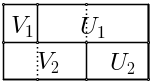
\includegraphics[width=2.4cm,height=1.2cm,scale=0.22]{diagram1C-1.png}\vspace{18pt}\PfEnd
\SepLine

\ProblemB{
	\TipsN{3}\,\,\,\TextB{Supp the intersec of any two of the vecsps $U,W,X,Y$ is $\zeroSubs.$}
	\IndentTipsN{3}\TextB{Give an exa that $\BigPar{X\oplus U}\,${\LARGE$\cap$}$\,\BigPar{Y\oplus W}\neq\zeroSubs.$}
}\Sbra{ Using notas in Chapter 2. } \;Let $B_X=\Par{e_1},B_U=\Par{e_2-e_1},B_Y=\Par{\,},B_W=\Par{e_2}.$
\SepLine

\ProblemB{
	\TipsN{4}\,\,\,\TextB{Let $V=U+W,\;I=U\cap W,\,U=I\oplus X,\,W=I\oplus Y.$ Prove $V=I\oplus\Par{X\oplus Y}.$}
}We show $X\cap Y=U\cap Y=W\cap X=\zeroSubs$ by ctradic.\parSol{}
$X\cap Y=\Delta\neq\zeroSubs\Rightarrow I=U\cap W\supseteq\Delta\Rightarrow I\cap X\neq\zeroSubs, I\cap Y\neq\zeroSubs.$\parSol{}
$U\cap Y=\Delta\neq\zeroSubs\Rightarrow I=U\cap W\supseteq\Delta\Rightarrow I\cap Y\neq\zeroSubs.$ Simlr for $W\cap X.$\parSol{\vspace{2pt}}
Thus $I+\Par{X+Y}=\Par{I\oplus X}\oplus Y=I\oplus\Par{X\oplus Y}.$\parSol{\vspace{2pt}}
Now we show $V=I+\Par{X+Y}.$ \;$\forall v\in V,v=u+w,\exists\,\Par{u,w}\in U\times W$\parSol{}
$\Rightarrow\exists\,\Par{i_u,x_u}\in I\times X,\,\Par{i_w,y_w}\in I\times Y,\;v=\Par{i_u+i_w}+x_u+y_w\in I+\Par{X+Y}.$\PfEnd
\SepLine

%\ProblemB{
%	\TipsN{3}\,\,\,\TextB{Let $V=U+W,\,I=U\cap W,\,U=I\oplus X,W=I\oplus Y.$ Prove $V=I\oplus\Par{X\oplus Y}.$}
%}Note that $V=\Par{I\oplus X}+\Par{I\oplus Y},$ and $X\cap Y=\zeroSubs.$\parSol{}
%\SepLine

%\ProblemN{\hypertarget{1C22}{22}}{
%	\TextNL{Supp $U=\Bra{\Par{x,y,x+y,x-y,2x}\in\Fbb^5}$.}
%	\TextNL{Find nonzero subsps $W_1,W_2,W_3$ of $\,\Fbb^5$ suth $\Fbb^5 = U\oplus W_1\oplus W_2\oplus W_3 $.}
%}\par\quad
%(1) Let $W_1=\Bra{\Par{0,0,z,0,0}\in\Fbb^5}\Rightarrow W_1\cap U=\zeroSubs.$ Now $U\oplus W_1=\Bra{\Par{x,y,z,x-y,2x}\in\Fbb^5}=U_1$.\par\quad
%(2) Let $W_2=\Bra{\Par{0,0,0,w,0}\in\Fbb^5}\Rightarrow W_2\cap U_1=\zeroSubs.$ Now $U_1\oplus W_2=\Bra{\Par{x,y,z,w,2x}\in\Fbb^5}=U_2$.\par\quad
%(3) Let $W_3=\Bra{\Par{0,0,0,0,u}\in\Fbb^5}\Rightarrow W_3\cap U_2=\zeroSubs.$ Now $U_2\oplus W_3=\Bra{\Par{x,y,z,w,u}\in\Fbb^5}=U_3$.\par\quad
%Thus $\Fbb^5=\BigPar{\Par{U\oplus W_1}\oplus W_2}\oplus W_3.$\PfEnd
%\SepLine

\ChEnd\pagebreak

\ChDecl{Ch2A}{2$\cdot$A}{}\orMode{\hLk{2A1}{1}\;\;\hLk{2A2}{2}\;\;\hLk{2A10}{10}\;\;\hLk{2A11}{11}\;\;\hLk{2A14}{14}\;\;\hLk{2A16}{16}\;\;\hLk{2A17}{17}\;\;|\;\;\hLk{2A4e314}{4E: 3,14}}{[1]: 1, (4E 3, 14), 2, 10; [2]: 11, 14, 16, 17.}

\vspace{6pt}

\ProblemN{\hypertarget{2A1}{1}}{
	\TextN{Prove [P] $\Par{v_1,v_2,v_3,v_4}$ spans $V\Longleftrightarrow\BigPar{v_1-v_2,v_2-v_3,v_3-v_4,v_4}$ also spans V [Q].}
}Note that $V=\Span{v_1,\dots,v_n}\Longleftrightarrow\forall v\in V,\exists\,a_1,\dots,a_n\in\Fbb,v=a_1v_1+\dots+a_nv_n.$\par\quad
Asum $\forall v\in V,\exists\,a_1,\dots,a_4,b_1,\dots,b_4\in\Fbb,$ \BigPar{ that is, if $\exists\,a_i,$ then we are to find $b_i,$ vice versa }\par\quad
$v=a_1 v_1+a_2 v_2+a_3 v_3+a_4 v_4=b_1\Par{v_1-v_2}+b_2\Par{v_2-v_3}+b_3\Par{v_3-v_4}+b_4 v_4$\par\quad
$\Blind{v}=b_1 v_1+\Par{b_2-b_1}v_2+\Par{b_3-b_2}v_3+\Par{b_4-b_3}v_4$\par\quad
$\Blind{v}=a_1\Par{v_1-v_2}+\Par{a_1+a_2}\Par{v_2-v_3}+\Par{a_1+a_2+a_3}\Par{v_3-v_4}+\Par{a_1+\dots+a_4}v_4.$\PfEnd
\SepLine

\ProblemB{
	\hypertarget{2A4e314}{}\TextB{Supp $\Par{v_1,\dots,v_m}$ is a list in $V$. For each $k$, let $w_k=v_1+\dots+v_k$.}
	(a) \TextB{Show $\Span{v_1,\dots,v_m}=\Span{w_1,\dots,w_m}.$}
	(b) \TextB{Show [P] $\Par{v_1,\dots,v_m}$ is liney indep $\Longleftrightarrow$ $\Par{w_1,\dots,w_m}$ is liney indep [Q].}
}\par\quad
(a) Asum $a_1v_1+\dots+a_mv_m=b_1w_1+\dots+b_mw_m=b_1v_1+\dots+b_k\Par{v_1+\dots+v_k}+\dots+b_m\Par{v_1+\dots+v_m}.$\par\quad\Ha
Then $a_k=b_k+\dots+b_m;\;\;a_{k+1}=b_{k+1}+\dots+b_m\Rightarrow b_k=a_k-a_{k+1};\;b_m=a_m.$ Simlr to Exe (1).\vspace{4pt}\par\quad
(b) $P\Rightarrow Q:\;\;b_1 w_1+\dots+b_m w_m=0=a_1 v_1+\dots+a_m v_m,\text{\;where\;}0=a_k=b_k+\dots+b_m.$\par\quad\Hb
$Q\Rightarrow P:\;\;a_1 v_1+\dots+a_m v_m=0=b_1 w_1+\dots+b_m w_m=0, \text{\;where\;} 0=b_m=a_m,\;0=b_k=a_k-a_{k+1}.$\vspace{4pt}\par\quad\Hb
\Or By (a), let $W=\Span{v_1,\dots,v_m}=\Span{w_1,\dots,w_m}.$ Supp $\Par{v_1,\dots,v_m}$ is liney dep.\par\quad\Hb
By [2.21](b), a list of len $\Par{m-1}$ spans $W.$ 又 By [2.23], $\Par{w_1,\dots,w_m}$ liney indep $\Rightarrow m\leqslant m-1.$\par\quad\Hb
Thus $\Par{w_1,\dots,w_m}$ is liney dep. Now rev the roles of $v$ and $w.$\PfEnd
\SepLine

\ProblemN{\hypertarget{2A2}{2}}{
	(a) \TextN{[P]\hspace{17pt}{\; A list $\Par{v}$ of len $1$ in $V$ is liney indep $\Longleftrightarrow v\neq 0.$} \hfill[Q]}
	(b) \TextN{[P]{\; A list $\Par{v,w}$ of len $2$ in $V$ is liney indep $\Longleftrightarrow\forall\lambda,\mu\in\Fbb,v\neq \lambda w,w\neq \mu v.$} \hfill[Q]\vspace{4pt}}
}(a) $Q\Rightarrow P:$ $v\neq 0\Rightarrow$ if $av=0$ then $a=0\Rightarrow\Par{v}$ liney indep.\parSol{\Ha}
$P\Rightarrow Q:$ $\Par{v}$ liney indep $\Rightarrow v\neq 0$, for if $v=0,$ then $av=0\notRightarrow a=0.$\parSol{\Ha}
${}^\neg Q\Rightarrow{}^\neg P:$ $v=0\Rightarrow av=0$ while we can let $a\neq 0\Rightarrow\Par{v}$ is liney dep.\parSol{\Ha}
${}^\neg P\Rightarrow{}^\neg Q:$ $\Par{v}$ liney dep $\Rightarrow av=0$ while $a\neq 0\Rightarrow v=0.$\parSol{\vspace{4pt}}
(b) $P\Rightarrow Q:$ $\Par{v,w}$ liney indep $\Rightarrow$  if $av+bw=0,$ then $a=b=0\Rightarrow$ no scalar multi.\parSol{\Hb}
$Q\Rightarrow P:$ no scalar multi $\Rightarrow$ if $av+bw=0,$ then $a=b=0\Rightarrow\Par{v,w}$ liney indep.\parSol{\Hb}
${}^\neg P\Rightarrow{}^\neg Q:$ $\Par{v,w}$ liney dep $\Rightarrow$ if $av+bw=0,$ then $a$ or $b\neq 0\Rightarrow$ scalar multi.\parSol{\Hb}
${}^\neg Q\Rightarrow{}^\neg P:$ scalar multi $\Rightarrow$ if $av+bw=0,$ then $a$ or $b\neq 0\Rightarrow$ liney dep.\PfEnd
\SepLine

\ProblemN{\hypertarget{2A10}{10}}{
	\TextNL{Supp $\Par{v_1,\dots,v_m}$ is liney indep in $V$ and $w\in V$.}
	\TextNL{Prove if $\BigPar{v_1+w,\dots,v_m+w}$ is linely depe, then $w\in\Span{v_1,\dots,v_m}$.}
}\par\quad
Note that $a_1\Par{v_1+w}+\dots+a_m\Par{v_m+w}=0\Rightarrow a_1 v_1+\dots+a_m v_m=-\Par{a_1+\dots+a_m}w.$\par\quad
Then $a_1+\dots+a_m\neq 0$, for if not, $a_1 v_1+\dots+a_m v_m=0$ while $a_i\neq 0$ for some $i$, ctradic.\par\quad
\Or We prove the ctrapos: Supp $w\not\in\Span{v_1,\dots,v_m}.$ Then $a_1+\dots+a_m=0.$\par\quad
Thus $a_1v_1+\dots+a_mv_m=0\Rightarrow a_1=\dots=a_m=0.$ Hence $\BigPar{v_1+w,\dots,v_m+w}$ is liney indep.\PfEnd\vspace{2pt}\quad
\Or $\exists\,j\in\Bra{1,\dots,m},v_j+w\in\Span{v_1+w,\dots,v_{j-1}+w}.$ If $j=1$ then $v_1+w=0$ and done.\par\quad
If $j\geqslant 2,$ then $\exists\,a_i\in\Fbb,v_j+w=a_1\Par{v_1+w}+\dots+a_{j-1}\Par{v_{j-1}+w}\Longleftrightarrow v_j+\lambda w=a_1 v_1+\dots+a_{j-1}v_{j-1}.$\par\quad
Where $\lambda=1-\Par{a_1+\dots+a_{j-1}}.$ Note that $\lambda\neq 0,$ for if not, $v_j+\lambda w=v_j\in\Span{v_1,\dots,v_{j-1}},$ ctradic.\par\quad
Now $w=\lambda^{-1}\Par{a_1 v_1+\dots+a_{j-1}v_{j-1}-v_j}\Rightarrow w\in\Span{v_1,\dots,v_m}.$\PfEnd
\SepLine

\ProblemN{\hypertarget{2A11}{11}}{
	\TextNL{Supp $\Par{v_1,\dots,v_m}$ is liney indep in $V$ and $w\in V$.}
	\TextNL{Show [P] $\Par{v_1,\dots,v_m,w}$ is liney indep $\Longleftrightarrow w\not\in\Span{v_1,\dots,v_m}$ [Q].}
}Equiv to $\Par{v_1,\dots,v_m,w}$ liney dep $\Longleftrightarrow w\in\Span{v_1,\dots,v_m}.$ Using [2.21]. Obviously.\PfEnd
\ANote (a) Supp $\Par{v_1,\dots,v_m,w}$ is liney indep. Then $\Par{v_1,\dots,v_m}$ liney indep $\Longleftrightarrow w\not\in\Span{v_1,\dots,v_m}.$\parNot
(b) Supp $\Par{v_1,\dots,v_m,w}$ is liney dep. Then $\Par{v_1,\dots,v_m}$ liney indep $\Longleftrightarrow w\in\Span{v_1,\dots,v_m}.$
\SepLine

\ProblemN{\hypertarget{2A14}{14}}{
	\TextNL{Prove [P] $V$ is infinide $\Longleftrightarrow\exists$ seq $\Par{v_1,v_2,\dots}$ in $V$ suth each $\Par{v_1,\dots,v_m}$ liney indep. [Q]}
}\par\quad
$P\Rightarrow Q:\;$ Supp $V$ is infinide, so that no list spans $V$.\par\quad
\Blind{$P\Rightarrow Q:\;$} {\tgbf Step 1}\;\; Pick a $v_1\neq 0,\Par{v_1}$ liney indep.\par\quad
\Blind{$P\Rightarrow Q:\;$} {\tgbf Step m}\; Pick a $v_m\not\in\Span{v_1,\dots,v_{m-1}},$ by Exe (11), $\Par{v_1,\dots,v_m}$ is liney indep.\par\quad
\Blind{$P\Rightarrow Q:\;$} This process recurly defines the desired seq $\Par{v_1,v_2,\dots}.$\vspace{4pt}\par\quad
${}^\neg P\Rightarrow{}^\neg Q:\;$ Supp $V$ is finide and $V=\Span{w_1 , ..., w_m}$.\par\quad
\Blind{${}^\neg P\Rightarrow{}^\neg Q:\;$} Let $\Par{v_1 , v_2 , \dots}$ be a seq in $V$, then $\Par{v_1,v_2,\dots,v_{m+1}}$ must be liney dep.\vspace{4pt}\par\quad
\Or\; $Q\Rightarrow P:\;$ Supp there is such a seq.\par\quad
\Blind{\Or\; $Q\Rightarrow P:\;$} Choose an $m$. Supp a liney indep list $\Par{v_1,\dots,v_m}$ spans $V$.\par\quad
\Blind{\Or\; $Q\Rightarrow P:\;$} Simlr to [2.16]. $\exists\,v_{m+1}\in V\Backslash\Span{v_1,\dots,v_m}.$ Hence no list spans $V.$\PfEnd
\SepLine

\ProblemN{\hypertarget{2A16}{16}}{
	\TextNL{Prove the vecsp of all continuous functions in $\Rbb^{[0,1]}$ is infinide.}
}Denote the vecsp by $U$.\par\quad
Choose one $m\in\Nbp.$ Supp $a_0,\dots,a_m\in\Rbb$ are suth $p\Par{x}=a_0+a_1 x+\dots+a_m x^m=0,\,\forall x\in\Sbra{0,1}.$\par\quad
Then $p$ has infily many roots and hence each $a_k=0,$ othws $\deg p\geqslant 0,$ ctradic [4.12].\par\quad
Thus $\Par{1,x,\dots,x^m}$ is liney indep in $\Rbb^{[0,1]}.$ Simlr to [2.16], $U$ is infinide.\PfEnd\vspace{8pt}\quad
\Or Note that\; $\Frac{\;1\;}{1}>\Frac{\;1\;}{2}>\dots>\Frac{\;1\;}{m},\,\,\,\forall m\in\Nbp.$ Supp\; $f_m=\MathLeftBrace{l}{
	\!x-{}${\Large$\frac{\;1\;}{m}$}$,\;\;x\in\Interval{(}{]}{${\Large$\frac{\;1\;}{m}$}$,\,1\,}\\
	\!0,\hfill x\in\Sbra{\,0,\,${\Large$\frac{\;1\;}{m}$}$\,}
}$\vspace{2pt}\par\quad
Then\; $f_1\XPar{${\Large$\frac{\;1\;}{m}$}$}=\dots=f_m\XPar{${\Large$\frac{\;1\;}{m}$}$}=0\neq f_{m+1}\XPar{${\Large$\frac{\;1\;}{m}$}$}.$ 
\;Hence $f_{m+1}\not\in\Span{f_1,\dots,f_m}.$ By Exe (14).\PfEnd
\SepLine

\ProblemN{\hypertarget{2A17}{17}}{
	\TextNL{Supp $p_0,p_1,\dots,p_m\in\PoF{m}$ suth $p_k\Par{2}=0$ for each $k\in\Bra{0,\dots,m}$.}
	\TextNL{Prove $\Par{p_0,p_1,\dots,p_m}$ is not liney indep in $\PoF{m}$.}
}\par\quad
Supp $\Par{p_0,p_1,\dots,p_m}$ is liney indep. Define $p\in\PoF{m}$ by $p\Par{z}=z.$\par\quad
\NOTICE that $\forall a_i\in\Fbb,z\neq a_0 p_0\Par{z}+\dots+a_m p_m\Par{z},$ for if not, let $z=2.$ Thus $z\not\in\Span{p_0,p_1,\dots,p_m}$.\par\quad
Then $\Span{p_0,p_1,\dots,p_m}\subsetneq\PoF{m}$ while the list $\Par{p_0,p_1,\dots,p_m}$ has len $\Par{m+1}$.\par\quad
Hence $\Par{p_0,p_1,\dots,p_m}$ is linely depe. For if not, then becs $\Par{1,z,\dots,z^m}$ of len $\Par{m+1}$ spans $\PoF{m},$\par\quad
by the steps in [2.23] trivially, $\Par{p_0,p_1,\dots,p_m}$ of len $\Par{m+1}$ spans $\PoF{m}.$ Ctradic.\PfEnd\vspace{6pt}\par\quad
\Or Note that $\PoF{m}=\Span{\underbrace{\;1,\;z,\;\dots,\;z^m\;}_{\text{of len }\SmallPar{m+1}}}.$ Then $\Par{p_0,p_1,\dots,p_m,z}$ of len $\Par{m+2}$ is liney dep.\vspace{2pt}\par\quad
As shown above,  $z\not\in\Span{p_0,p_1,\dots,p_m}.$ And hence by [2.21](a), $\Par{p_0,p_1,\dots,p_m}$ is liney dep.\PfEnd
\SepLine
\ChEnd\pagebreak

\ChDecl{Ch2B}{2$\cdot$B}{}\orMode{\hLk{2B1}{1}\;\;\hLk{2B8}{8}\;\;|\;\;\hLk{2B4e5}{4E:\;\;5}\;\;\hLk{2B4e9}{9}\;\;\hLk{2B4e11}{11}}{[1]: 7, 1, (4E 9); [2]: (4E 5), 8, (4E 11).}
\vspace{8pt}

%\ProblemN{\hypertarget{2B7}{7}}{
%	\TextN{Prove or give a counterexa\hspace{1pt}$:$ If $\Par{v_1,v_2,v_3,v_4}$ is a bss of $V$ and $U$ is a subsp of $V$}
%	\TextN{suth $v_1,v_2\in U$ and $v_3\not\in U$ and $v_4\not\in U$, then $\Par{v_1,v_2}$ is a bss of U.}
%}A counterexa\hspace{1pt}: Let $V=\Rbb^4$ and $B_V=\Par{e_1,e_2,e_3,e_4}$ be std bss.\par\quad
%Let $v_1=e_1,v_2=e_2,v_3=e_3+e_4,v_4=e_4.$ Then $\Par{v_1,\dots,v_4}$ is a bss of $\Rbb^4.$\par\quad
%Let $U=\Span{e_1,e_2,e_3}=\Span{v_1,v_2,v_3-v_4}.$ Then $v_3\not\in U$ and $\Par{v_1,v_2}$ is not a bss of $U.$\PfEnd\quad
%\AComm Let $W=\Span{v_4-v_1}.$ Then $v_4\in V=U\oplus W$ but $W\not\ni v_4\not\in U.$
%\SepLine

\ProblemB[]{
	\Tips \,\,\,\TextB{Supp $\dim V=n,$ and $U$ is a subsp of $V$ with $U\neq V.$}
	\IndentTips\TextB{Prove $\exists\,B_V=\Par{v_1,\dots,v_n}$ suth each $v_k\not\in U.$}
}\TextB{\vspace{0pt}}
Note that $U\neq V\Rightarrow n\geqslant 1.$ We will construct $B_V$ via the following process.\TextB{}
{\tgbfx Step 1.} $\exists\,v_1\in V\Backslash U\Rightarrow v_1\neq 0.$ If $\Span{v_1}=V$ then we stop.\TextB{}
{\tgbfx Step k.} Supp $\Par{v_1,\dots,v_{k-1}}$ is liney indep in $V,$ each of which belongs to $V\Backslash U.$\TextB{}
\Blind{\tgbfx Step k.} Note that $\Span{v_1,\dots,v_{k-1}}\neq V.$ And if $\Span{v_1,\dots,v_{k-1}}\cup U=V,$ then by (1.C.12),\TextB{}
\Blind{\tgbfx Step k.} \Sbra{ becs $\Span{v_1,\dots,v_{k-1}}\not\subseteq U,$ } $U\subseteq \Span{v_1,\dots,v_{k-1}}\Rightarrow\Span{v_1,\dots,v_{k-1}}=V.$\TextB{}
\Blind{\tgbfx Step k.} Hence becs $\Span{v_1,\dots,v_{k-1}}\neq V,$ it must be case that $\Span{v_1,\dots,v_{k-1}}\cup U\neq V.$\TextB{}
\Blind{\tgbfx Step k.} Thus $\exists\,v_k\in V\Backslash U$ suth $v_k\not\in\Span{v_1,\dots,v_{k-1}}.$\TextB{}
\Blind{\tgbfx Step k.} By (2.A.11), $\Par{v_1,\dots,v_k}$ is liney indep in $V$. If $\Span{v_1,\dots,v_k}=V,$ then we stop.\TextB{}
Becs $V$ is finide, this process will stop after $n$ steps.\PfEnd\vspace{4pt}\TextB{}
\Or Supp $U\neq\zeroSubs.$ Let $B_U=\Par{u_1,\dots,u_m}.$ Extend to a bss $\Par{u_1,\dots,u_n}$ of $V.$\TextB{}
\Blind{\Or}Then let $B_V=\Par{u_1-u_k,\dots,u_m-u_k,u_{m+1},\dots,u_k,\dots,u_n}.$\PfEnd
\SepLine

\ProblemN{\hypertarget{2B1}{1}}{
	\TextN{Find all vecsps on whatever $\Fbb$ that have exactly one bss.}
}The trivial vecsp $\zeroSubs$ will do. Indeed, the only bss of $\zeroSubs$ is the empty list $\Par{\,}$.\parSol{}
Now consider the field $\Bra{0,1}$ containing only the add id and multi id,\parSol{}
with $1+1=0.$ Then the list $\Par{1}$ is the uniq bss. Now the vecsp $\Bra{0,1}$ will do.\parSol{}
\AComm All vecsp on such $\Fbb$ of dim $1$ will do.\parSol{}
Consider other $\Fbb.$ Note that this $\Fbb$ contains at least and strictly more than $0$ and $1.$ Failed.\PfEnd
\SepLine

\ProblemBnoor{\hypertarget{2B4e9}{4E 9}}{
	\TextB{Supp $\Par{v_1,\dots,v_m}$ is a list in $V$. For $k\in\Bra{1,\dots,m}$, let $w_k=v_1+\dots+v_k.$}
	\TextB{Show [P] $B_V=\Par{v_1,\dots,v_m}\Longleftrightarrow B_V=\Par{w_1,\dots,w_m}.$ [Q]}
}\NOTICE that $B_U=\Par{u_1,\dots,u_n}\Longleftrightarrow\forall u\in U,\exists\,!\,a_i\in\Fbb,u=a_1 u_1+\dots+a_n u_n.$\par\quad
$P\Rightarrow Q:\forall v\in V,\exists\,!\,a_i\in\Fbb,\;v=a_1 v_1+\dots+a_m v_m\Rightarrow v=b_1 w_1+\dots+b_m w_m,\exists\,!\,b_k=a_k-a_{k+1},b_m=a_m.$\vspace{2pt}\par\quad
$Q\Rightarrow P:\forall v\in V,\exists\,!\,b_i\in\Fbb,\;v=b_1w_1+\dots+b_mw_m\Rightarrow v=a_1v_1+\dots+a_mv_m,\exists\,!\,a_k=\sum_{j=k}^m b_j.$\PfEnd\vspace{3pt}
\AComm \Or Using \Sbra{3.C {\NOTEFOR} [3.30, 32](a)}.
\SepLine

\ProblemBnoor{\hypertarget{2B4e5}{4E 5}}{
	\TextB{Supp $U,W$ are finide, $V=U+W,\;B_U=\Par{u_1,\dots,u_m},\;B_W=\Par{w_1,\dots,w_n}.$}
	\TextB{Prove $\exists\,B_V$ consisting of vecs in $U\cup W$.\vspace{-4pt}}
}$V=\Span{u_1,\dots,u_m}+\Span{w_1,\dots,w_n}=\Span[\BigPar]{\overbrace{u_1,\dots,u_m,w_1,\dots,w_n}^{\text{Reduce}}}.$ By [2.31].\PfEnd
\SepLine

\ProblemN{\hypertarget{2B8}{8}}{
	\TextN{Supp $V=U\oplus W,\;B_U=\Par{u_1,\dots,u_m},\;B_W=\Par{w_1,\dots,w_n}.$}
	\TextN{Prove $B_V=\BigPar{u_1,\dots,u_m,w_1,\dots,w_n}$.}
}$\forall v\in V,\exists\,!\,u\in U,w\in W\Rightarrow\exists\,!\,a_i,b_i\in\Fbb,v=u+w=\sum_{i=1}^ma_iu_i+\sum_{i=1}^nb_iw_i.$\parSol{}
\Or\;$V=\Span{u_1,\dots,u_m}\oplus\Span{w_1,\dots,w_n}=\Span[\BigPar]{u_1,\dots,u_m,w_1,\dots,w_n}.$\parSol{\vspace{2pt}}
\Blind{\Or\;}Note that $\sum_{i=1}^ma_iu_i+\sum_{i=1}^nb_iw_i=0\Rightarrow\sum_{i=1}^ma_iu_i=-\sum_{i=1}^nb_iw_i\in U\cap W=\zeroSubs.$\PfEnd
\SepLine\pagebreak

\BulletPointX\NoteFor{{\tgsc liney indep seq and }[2.34]}\;\;$“V=\Span{v_1,\dots,v_n,\dots}”$ is an invalid expr.\TextB{}
If we allow using $“$infini list$”$, then we must assure that $\Par{v_1,\dots,v_n,\dots}$ is a spanning $“$list$”$\TextB{}
suth $\forall v\in V,\exists$ smallest $n\in\Nbp,\;v=a_1 v_1+\dots+a_n v_n.$ Moreover, given a list $\Par{w_1,\cdots,w_n,\cdots}$ in $W,$\TextB{}
we can prove $\exists\,!\,T\in\Lm{V,W}$ with each $Tv_k=w_k,$ which has less restr than [3.5].\TextB{}
But the key point is, how can we assure that such a $“$list$”$ exis. \colorbox{yellow}{TODO: More details.}
%\TextB{}
%\TextB{}
\SepLine

\ProblemBnoor[]{\hypertarget{2B4e}{9.A.3,4 \OR 4E 11}}{
	\TextB{Supp $V$ is on $\Rbb,$ and $v_1,\dots,v_n\in V.$ Let $B=\Par{v_1,\dots,v_n}.$\vspace{2pt}}
	(a) \TextB{Show [P] $B$ is liney indep in $V$ $\Longleftrightarrow B$ is liney indep in $V_{\!\Cbb}.$ [Q]}
	(b) \TextB{Show [P] $B$ spans $V$ $\Longleftrightarrow B$ spans $V_{\!\Cbb}.$ [Q]\vspace{2pt}}
}{\FontSmall\par\quad
(a) $P\Rightarrow Q:$ \;Note that each $v_k\in V_{\!\Cbb}.$ \;\; $Q\Rightarrow P:$ \;If $\lambda_k\in\Rbb$ with $\lambda_1v_1+\dots+\lambda_nv_n=0,$ then each $\Real\lambda_k=\lambda_k=0.$\par\quad
\Blind{(a)} ${}^\neg P\Rightarrow{}^\neg Q:$ \;$\exists\,v_j=a_{j-1}v_{j-1}+\dots+a_1v_1\in V_{\!\Cbb}.$\par\quad
\Blind{(a)} ${}^\neg Q\Rightarrow{}^\neg P:$ \;$\exists\,v_j=\lambda_{j-1}v_{j-1}+\dots+\lambda_1v_1\Rightarrow v_j=\Par{\Real\lambda_{j-1}}v_{j-1}+\dots+\Par{\Real\lambda_1}v_1\in V.$\par\vspace{3pt}\quad
(b) $P\Rightarrow Q:$ \;$\forall u+\i v\in V_{\!\Cbb},\;u,v\in V\Rightarrow\exists\,a_i,b_i\in\Rbb,u+\i v=\sum_{i=1}^n\Par{a_i+\i b_i}v_i.$\par\quad
\Blind{(b)} $Q\Rightarrow P:$ \;$\forall v\in V,\exists\,\!\,a_i+\i b_i\in\Cbb,\;v+\i 0=\envFontDefault\BigPar{\!\sum_{i=1}^na_iv_i}+\i\,\BigPar{\!\sum_{i=1}^nb_iv_i}\envFontSmall\Rightarrow v\in\Span{v_1,\dots,v_m}.$\par\quad
\Blind{(b)} ${}^\neg Q\Rightarrow{}^\neg P:$ \;$\exists\,v\in V,v\not\in\Span{B}\Rightarrow v+\i 0\not\in\Span{B}$ while $v+\i 0\in V_{\!\Cbb}.$\par\quad
\Blind{(b)} ${}^\neg Q\Rightarrow{}^\neg P:$ \;$\exists\,u+\i v\in V_{\!\Cbb},u+\i v\not\in\Span B\Rightarrow u$ or $v\not\in\Span B.$ Note that $u,v\in V.$
}\PfEnd\vspace{-4pt}
\SepLine

\ChEnd\vspace{-4pt}

\vfill\ChDecl{Ch2C}{2$\cdot$C}{}\orMode{\hLk{2C1}{1}\;\;\hLk{2C7}{7}\;\;\hLk{2C9}{9}\;\;\hLk{2C10}{10}\;\;\hLk{2C14}{14,16}\;\;\hLk{2C15}{15}\;\;\hLk{2C17}{17}\;\;|\;\;\hLk{2C4e10}{4E:\;\;10}\;\;\hLk{2C4e14}{14,15}\;\;\hLk{2C4e16}{16}}{[1]: 15; [2]: 1, 7, 9, (4E 16); [3]: 10; [4]: (4E 10), 14, 16; [5]: 17, (4E 14, 15).}

\vspace{4pt}

\ProblemN{\hypertarget{2C15}{15}}{
	\TextNL{Supp $\dim V=n\geqslant 1.$ Prove $\exists\,1$-dim subsps $V_{\!1},\dots,V_{\!n}$ suth $V=V_{\!1}\oplus \dots\oplus V_{\!n}.$}
}Supp $B_V=\Par{v_1,\dots,v_n}.$ Define $V_{\!i}$ by $V_{\!i}=\Span{v_i}$ for each $i\in\Bra{1,\dots,n}.$\parSol{}
Then $\forall v\in V,\exists\,!\,a_i\in\Fbb,v=a_1 v_1+\dots+a_n v_n\Rightarrow\exists\,!\,u_i\in V_{\!i},v=u_1+\dots+u_n$\PfEnd
\SepLine

\ProblemBnoor{\NoteForSmall{Exe (15)}}[]{
	\TextB{Supp $v\in V\nonzero.$ Prove $\exists\,B_V=\Par{v_1,\dots,v_n},v=v_1+\dots+v_n.$}
}If $n=1$ then let $v_1=v$ and done. Supp $n>1.$\parSol{}
Extend $\Par{v}$ to a bss $\Par{v,v_1,\dots,v_{n-1}}$ of $V.$ Let $v_n=v-v_1-\dots-v_{n-1}.$\parSol{}
又 $\Span{v,v_1,\dots,v_{n-1}}=\Span{v_1,\dots,v_n}.$ Hence $\Par{v_1,\dots,v_n}$ is also a bss of $V.$\PfEnd\vspace{4pt}
\AComm Let $B_V=\Par{v_1,\dots,v_n}$ and supp $v=u_1+\dots+u_n,$ where each $u_i=a_i v_i\in V_{\!i}.$\parCom
But $\Par{u_1,\dots,u_n}$ might not be a bss, becs there might be some $u_i=0.$\vspace{-2pt}
\SepLine\pagebreak

\ProblemNnoor[]{\hypertarget{2C1}{1}}{{\COROLLARY} for [2.38,39]}{
	\TextN{Supp $U$ is a subsp of $V$ suth $\dim V=\dim U$. Then $V=U.$}
}\Blind{\IndentN} Let $B_U=\Par{u_1,\dots,u_m}.$ Then $m=\dim V.$ 又 $u_i\in V.$ By [2.39], $B_V=\Par{u_1,\dots,u_m}.$\PfEnd\vspace{-2pt}
\SepLine[-2pt]

\ProblemB[]{
	Let $v_1,\dots,v_n\in V$ and $\dim\Span{v_1,\dots,v_n}=n.$ Then $\Par{v_1,\dots,v_n}$ is a bss of $\Span{v_1,\dots,v_n}.$\TextB{}
	{\tgsl Notice that $\Par{v_1,\dots,v_n}$ is a spanning list of $\Span{v_1,\dots,v_n}$ of len $n=\dim\Span{v_1,\dots,v_n}.$}\TextB{\vspace{-4pt}}
}\SepLine

\ProblemN{\hypertarget{2C7}{7}}{
	(a) \TextN{Let $U=\Bra{p\in\PoF{4}:p\Par{2}=p\Par{5}=p\Par{6}}$. Find a bss of $U$.}
	(b) \TextN{Extend the bss in {\tgnr(b)} to a bss of $\PoF{4}$.}
	(c) \TextN{Find a subsp $W$ of $\PoF{4}$ suth $\PoF{4}=U\oplus W$.}
}Using Exe (10).
%Supp $p\Par{z}=az^4+bz^3+cz^2+dz+e$ suth $p\Par{2}=p\Par{5}=p\Par{6}$.\vspace{4pt}\par\quad
%Then $\hMath[0pt]{r}{\left|}{\right\}}{
	%	p\Par{2}=16a+8b+4c+2d+e\,\;\;\Par{\text{I}}\;\;\\
	%	p\Par{5}=625a+125b+25c+5d+e\;\;\Par{\text{II}}\,\;\\
	%	p\Par{6}=1296a+216b+36c+6d+e\;\,\Par{\text{III}}
	%}\Rightarrow\MathLeftBrace{l}{
	%	\Par{\text{II}}\;-\;\Par{\text{I}}=0\\
	%	\Par{\text{III}}-\Par{\text{II}}=0\\
	%	\Par{\text{III}}-\;\Par{\text{I}}=0\\
	%}$\vspace{4pt}\par\quad
%{\tgsl You don't have to compute to know that the dimension of the set of solutions is 3.}
\par\quad
\NOTICE that $\not\exists\,p\in\PoFi$ of deg $1$ and $2,$ while $p\in U.$ Thus $\dim U\leqslant \dim\PoF{4}-2=3.$\par\vspace{2pt}\quad
(a) Consider $B=\envFontLarge\BigPar{\envFontDefault1,\Par{z-2}\Par{z-5}\Par{z-6},z\Par{z-2}\Par{z-5}\Par{z-6}\envFontLarge}.$\par\quad\Ha
Let $a_0+a_3\Par{z-2}\Par{z-5}\Par{z-6}+a_4z\Par{z-2}\Par{z-5}\Par{z-6}=0\Rightarrow a_0=a_3=a_4=0.$\par\quad\Ha
Thus the list $B$ is liney indep in $U.$ Now $\dim U\geqslant 3\Rightarrow \dim U=3.$ Thus $B_U=B.$\par\vspace{2pt}\quad
(b) Extend to a bss of $\PoF{4}$ as $\envFontLarge\BigPar{\envFontDefault 1,z,z^2,\Par{z-2}\Par{z-5}\Par{z-6},z\Par{z-2}\Par{z-5}\Par{z-6}\envFontLarge}.$\par\quad
(c) Let $W=\Span{z,z^2}=\Bra{az+bz^2:a,b\in\Fbb}$, so that $\PoF{4}=U\oplus W.$\PfEnd
\SepLine

\ProblemN{\hypertarget{2C9}{9}}{
	\TextN{Supp $\Par{v_1,\dots,v_m}$ is liney indep in $V,w\in V.$ Prove $\dim\Span[\BigPar]{v_1+w,\dots,v_m+w}\geq m-1$.}
}Using the result of (2.A.10, 11).\par\quad
Note that $v_i-v_1=\Par{v_i+w}-\Par{v_1+w}\in\Span{v_1+w,\dots,v_n+w},$ for each $i=1,\dots,m$.\par\quad
$\Par{v_1,\dots,v_m}$ liney indep $\Rightarrow$ $\BigPar{v_1,v_2-v_1,\dots,v_m-v_1}$ liney indep $\Rightarrow$ $\underbrace{\BigPar{v_2-v_1,_{}\dots,v_m-v_1}}_{\text{of len }\Par{m-1}}$ liney indep.\vspace{-15pt}\par\quad
又 If $w\not\in\Span{v_1,\dots,v_m}.$ Then $\BigPar{v_1+w,\dots,v_m+w}$ is liney indep.\par\quad
Hence $m\geqslant\dim\Span[\BigPar]{v_1+w,\dots,v_m+w}\geq m-1.$\PfEnd
\SepLine

\ProblemBnoor{\hypertarget{2C4e16}{4E 16}}{
	\TextB{Supp $V$ is finide, $U$ is a subsp of $V$ with $U\neq V$. Let $n=\dim V,m=\dim U$.}
	\TextB{Prove $\exists\,\Par{n-m}$ subsps  $U_1,\dots,U_{n-m}$, each of dim $\Par{n-1}$, suth $\bigcap\limits_{i=1}^{n-m}U_i=U$.}
}Let $B_U=\Par{v_1,\dots,v_m},\;B_V=\BigPar{v_1,\dots,v_m,u_1,\dots,u_{n-m}}$.\parSol{}
Define $U_i=\Span[\BigPar]{v_1,\dots,v_m,u_1,\dots,u_{i-1},u_{i+1},\dots,u_{n-m}}$ for each $i$. Then $U\subseteq U_i$ for each $i.$\vspace{4pt}\parSol{}
And becs $\forall v\in \bigcap\limits_{i=1}^{n-m}U_i,v=v_0+b_1 u_1+\dots+b_{n-m} u_{n-m}\in U_i\Rightarrow$ each $b_i=0\Rightarrow v\in U.$\vspace{-4pt}\parSol{}
Hence $\bigcap\limits_{i=1}^{n-m}U_i\subseteq U.$\PfEnd
%\vspace{10pt}
%\AExa {Supp $\dim V=6,\dim U=3$.\par\vspace{2pt}\quad
%	$\Par{\overbrace{\underbrace{v_1,v_2,v_3}_\text{Bss of U},v_4,v_5,v_6}^\text{Bss of V}},$ define $\hMath[0pt]{l}{\left|}{\right\}}{$
%		$U_1=\Span{v_1,v_2,v_3}\oplus\Span{v_5,v_6}\\ $
%		$U_2=\Span{v_1,v_2,v_3}\oplus\Span{v_4,v_6}\\ $
%		$U_3=\Span{v_1,v_2,v_3}\oplus\Span{v_4,v_5}$
%		$}\Rightarrow\dim U_i=6-1,\,\,i=\underbrace{1,2,3}_{6-3=3}.$}
%\PfEnd[-10pt]\vspace{-4pt}
\SepLine

\BulletPointX\NoteForSmall{Exe 10} \,\,\,For each nonconst $p\in\Span{1,z,\dots,z^m},\;\exists$ smallest $m\in\Nbp,$ which is $\deg p.$\TextB{}
(a) If $p_0,p_1,\dots,p_m$ are suth all $a_{k,k}\neq 0,$ and\TextB{}
\Hb $p_0=a_{0,0},\,$ each $p_k=a_{0,k}+a_{1,k}z+\dots+a_{k,k}z^k.$\TextB{\vspace{-18pt}}
\Ha Then the upper-trig $\Mt[\envFontLarge\BigPar]{\envFontDefault I,\Par{p_0,p_1,\dots,p_m},\Par{1,z,\dots,z^m}\envFontLarge}={}${\small$\begin{pmatrix}
		a_{0,0} & a_{0,1} & \cdots & a_{0,m}\\
		0       & a_{1,1} & \cdots & a_{1,m}\\
		\vdots  & \vdots  & \ddots & \vdots\\
		0       & 0       & \cdots & a_{m,m}
	\end{pmatrix}$}.\TextB{\vspace{-8pt}}
(b) If $p_0,p_1,\dots,p_m$ are suth all $a_{k,k}\neq 0,$ and\TextB{}
\Hb $p_0=a_{0,0}+\dots+a_{m,0}x^m,\,$ each $p_k=a_{k,k}x^k+\dots+a_{m,k}x^m.$\TextB{\vspace{-18pt}}
\Hb Then the lower-trig \;$\Mt[\envFontLarge\BigPar]{\envFontDefault I,\Par{p_0,p_1,\dots,p_m},\Par{1,z,\dots,z^m}\envFontLarge}={}${\small$\begin{pmatrix}
		a_{0,0} & 0       & \cdots & 0\\
		a_{1,0} & a_{1,1} & \cdots & 0\\
		\vdots  & \vdots  & \ddots & \vdots\\
		a_{m,0} & a_{m,1} & \cdots & a_{m,m}
	\end{pmatrix}$}.\TextB{\vspace{-12pt}}
\AComm Define $\xi_k\Par{p}$ by the coeff of $z^k$ in $p\in\PoF{m}.$\parCom\IndentB{}
Then $\Mt[\envFontLarge\BigPar]{\envFontDefault\xi_k,\Par{1,z,\dots,z^m},\Par{1}\envFontLarge}=\mathcal{E}^{\SmallPar[1pt]{1,k}}\in\Fbb^{1,m+1}.$\vspace{-2pt}
\SepLine\pagebreak

\ProblemN{\hypertarget{2C10}{10}}{
	\TextNL{Supp $m\in\Nbp,\;p_0,p_1,\dots,p_m\in\PoFi$ are suth each $\deg p_k=k.$}
	\TextNL{Prove $\Par{p_0,p_1,\dots,p_m}$ is a bss of $\PoF{m}$.}
}{Using induc on $m$.}\par\quad
(i) {$k=1.$ \;$\deg p_0=0;\;\deg p_1=1\Rightarrow\Span[\BigPar]{p_0,p_1}=\Span[\BigPar]{1,x}.$}\par\vspace{2pt}\quad\Endi
(ii) {$1\leqslant k\leqslant m-1.$ \;Asum $\Span[\BigPar]{p_0,p_1,\dots,p_k}=\Span[\BigPar]{1,x,\dots,x^k}.$}\par\quad\Hii
{Then $\Span[\BigPar]{p_0,p_1,\dots,p_k,p_{k+1}}\subseteq\Span[\BigPar]{1,x,\dots,x^k,x^{k+1}}$.}\par\vspace{2pt}\quad\Hii
{又 $\deg p_{k+1}=k+1,\;\;p_{k+1}\Par{x}=a_{k+1}x^{k+1}+r_{k+1}\Par{x};\;\;a_{k+1}\neq 0,\;\;\deg r_{k+1}\leqslant k.$}
\par\vspace{2pt}\quad\Hii
{$\Rightarrow x^{k+1}=\Frac{1}{a_{k+1}}\XPar{p_{k+1}\Par{x}-r_{k+1}\Par{x}}\in\Span[\BigPar]{1,x,\dots,x^k,p_{k+1}}=\Span[\BigPar]{p_0,p_1,\dots,p_k,p_{k+1}}$.}\par\vspace{2pt}\quad\Hii
{$\therefore\,\,x^{k+1}\in\Span[\BigPar]{p_0,p_1,\dots,p_k,p_{k+1}}\Rightarrow\Span[\BigPar]{1,x,\dots,x^k,x^{k+1}}\subseteq\Span[\BigPar]{p_0,p_1,\dots,p_k,p_{k+1}}$.}\par\vspace{2pt}\quad
{Thus $\PoF{m}=\Span[\BigPar]{1,x,\dots,x^m}=\Span[\BigPar]{p_0,p_1,\dots,p_m}.$}\FontNorm\PfEnd\vspace{8pt}\quad
\Or 用比较系数法. {Denote the coeff of $x^k$ in $p\in\PoFi$ by $\xi_k\Par{p}.$}\par\quad
{Supp $L=a_m p_m\Par{x}+\dots+a_1 p_1\Par{x}+a_0p_0\Par{x}=0\cdot x^m+\dots+0\cdot x+0\cdot 1=R,\forall x\in\Fbb.$}\par\quad
{We show $a_m=\dots=a_0=0$ via the following process. So that $\Par{p_0,p_1,\dots,p_m}$ is liney indep.}\vspace{2pt}\par\quad
{\tgbfx Step 1.} {For $k=m,$ \;$\xi_{m}\Par{L}=a_{m}\xi_{m}\Par{p_m}=\xi_{m}\Par{R}=0$ 又 $\deg p_m=m,\;\xi_{m}\Par{p_m}\neq 0\Rightarrow a_m=0.$}\par\quad
\Blind{{\tgbfx Step 1.}} {Now $L=a_{m-1}p_{m-1}\Par{x}+\dots+a_0p_0\Par{x}.$}\vspace{2pt}\par\quad
{\tgbfx Step k.} {For $0\leqslant k\leqslant m,$ we have $a_m=\dots=a_{k+1}=0.$}\par\quad
\Blind{{\tgbfx Step k.}} {Now $\xi_{k}\Par{L}=a_{k}\xi_{k}\Par{p_k}=\xi_{k}\Par{R}=0$ 又 $\deg p_k=k,\;\xi_{k}\Par{p_k}\neq 0\Rightarrow a_k=0.$}\par\quad
\Blind{{\tgbfx Step k.}} {Now if $k=0,$ then done. Othws, we have $L=a_{k-1}p_{k-1}\Par{x}+\dots+a_0p_0\Par{x}.$}\PfEnd
\SepLine

\ProblemBnoor{\Tips}[]{
	\TextB{Supp $m\in\Nbp,\;p_0,p_1,\dots,p_m\in\PoF{m}$ are suth the lowest term of each $p_k$ is of deg $k.$}
	\Blind{\Tips} \TextB{Prove $\Par{p_0,p_1,\dots,p_m}$ is a bss of $\PoF{m}.$}
}{Using induc on $m.$\par}\quad
{Let each $p_k$ be defined by $p_k\Par{x}=a_{k,k} x^k+\dots+a_{m,k} x^m,$ where $a_{k,k}\neq 0.$\par}\quad
(i) {$k=1.$ \;$p_m\Par{x}=a_{m,m}x^m;\;p_{m-1}\Par{x}=a_{m-1,m-1}x^{m-1}+a_{m,m-1}x^m\Longrightarrow\Span[\BigPar]{x^m,x^{m-1}}=\Span[\BigPar]{p_m,p_{m-1}}.$\par}\vspace{2pt}\quad\Endi
(ii) {$1\leqslant k\leqslant m-1.$ \;Asum $\Span[\BigPar]{x^m,\dots,x^{m-k}}=\Span[\BigPar]{p_m,\dots,p_{m-k}}.$}\par\quad\Hii
{Then $\Span[\BigPar]{p_m,\dots,p_{m-\SmallPar{k+1}}}\subseteq\Span[\BigPar]{x^m,\dots,x^{m-\SmallPar{k+1}}}.$\par}\quad\Hii
{又 $p_{m-\SmallPar{k+1}}$ has the form $a_{m-\SmallPar{k+1},m-\SmallPar{k+1}}x^{m-\SmallPar{k+1}}+r_{m-\SmallPar{k+1}}\Par{x};\;$\par}\quad\Hii
{\Blind{又} where the lowest term of $r_{m-\SmallPar{k+1}}\in\PoF{m}$ is of deg $\Par{m-k}.$\par}\vspace{24pt}\quad\Hii
{\Blind{$\Rightarrow x^{m-\SmallPar{k+1}}=\Frac{}{a_{m-\SmallPar{k+1},m-\SmallPar{k+1}}}\XPar{p_{m-\SmallPar{k+1}}\Par{x}-r_{m-\SmallPar{k+1}}\Par{x}}$}${}=\Span[\BigPar]{p_m,\dots,p_{m-k},p_{m-\SmallPar{k+1}}}.$\par}\vspace{-50pt}\quad\Hii
{$\Rightarrow x^{m-\SmallPar{k+1}}=\Frac{1}{a_{m-\SmallPar{k+1},m-\SmallPar{k+1}}}\XPar{p_{m-\SmallPar{k+1}}\Par{x}-r_{m-\SmallPar{k+1}}\Par{x}}\in\Span[\BigPar]{x^m,\dots,x^{m-k},p_{m-\SmallPar{k+1}}}$\par}\vspace{4pt}\quad\Hii
{$\therefore\;x^{m-\SmallPar{k+1}}\in\Span[\BigPar]{p_m,\dots,p_{m-k},p_{m-\SmallPar{k+1}}}$\par}\vspace{3pt}\quad\Hii
{\Blind{$\therefore\;$}$\Rightarrow\Span[\BigPar]{x^m,\dots,x^{m-k},x^{m-\SmallPar{k+1}}}\subseteq\Span[\BigPar]{p_m,\dots,p_{m-k},p_{m-\SmallPar{k+1}}}.$\par}\vspace{3pt}\quad
{Thus $\PoF{m}=\Span[\BigPar]{x^m,\dots,x,1}=\Span[\BigPar]{p_m,\dots,p_1,p_0}.$}\PfEnd\vspace{8pt}\quad
\Or 用比较系数法. {Denote the coeff of $x^k$ in $p\in\PoFi$ by $\xi_k\Par{p}.$}\par\quad
{Supp $L=a_m p_m\Par{x}+\dots+a_1 p_1\Par{x}+a_0p_0\Par{x}=0\cdot x^m+\dots+0\cdot x+0\cdot 1=R,\forall x\in\Fbb.$}\par\quad
{We show $a_m=\dots=a_0=0$ via the following process. So that $\Par{p_0,p_1,\dots,p_m}$ is liney indep.}\vspace{2pt}\par\quad
{\tgbfx Step 1.} {For $k=0,$ \;$\xi_{0}\Par{L}=a_{0}\xi_{0}\Par{p_0}=\xi_{0}\Par{R}=0$ 又 $\deg p_0=0,\;\xi_{0}\Par{p_0}\neq 0\Rightarrow a_0=0.$}\par\quad
\Blind{{\tgbfx Step 1.}} {Now $L=a_1p_1\Par{x}+\dots+a_{m}p_{m}\Par{x}.$}\vspace{2pt}\par\quad
{\tgbfx Step k.} {For $0\leqslant k\leqslant m,$ we have $a_{k-1}=\dots=a_0=0.$}\par\quad
\Blind{{\tgbfx Step k.}} {Now $\xi_{k}\Par{L}=a_{k}\xi_{k}\Par{p_k}=\xi_{k}\Par{R}=0$ 又 $\deg p_k=k,\;\xi_{k}\Par{p_k}\neq 0\Rightarrow a_k=0.$}\par\quad
\Blind{{\tgbfx Step k.}} {Now if $k=m,$ then done. Othws, we have $L=a_{k+1}p_{k+1}\Par{x}+\dots+a_mp_m\Par{x}.$}\PfEnd
\SepLine

\BulletPointX\NoteForSmall{[2.11]} {\tgsc Good definition for a general term always aviods undefined behaviours.}\TextB{}
If $\deg p=0,$ then $p\Par{z}=a_0\neq 0,$ but \uline{not literally $a_0z^0,$} by which if $p$ is defined, then it comes to $0^0.$\TextB{}
To make it clear, we \uline{specify that {\tgsl in} $\PoFi,$ $a_0z^0=a_0,$ where $z^0$ appears just for nota conveni.}\TextB{}
Becs by def, the term $a_0z^0$ in a poly only represents the const term of the poly, which is $a_0.$\TextB{}
For conveni, we asum $z^0=1$ in formula deduction and poly def. Absolutely without $0^0.$
\SepLine

\ProblemBnoor{\hypertarget{2C4e10}4E 10}{
	\TextB{Supp $m$ is a positive integer. For $0\leqslant k\leqslant m$, let $p_k\Par{x}=x^k\Par{1-x}{^{m-k}}$.}
	\TextB{Show $\Par{p_0,\dots,p_m}$ is a bss of $\PoF{m}$.\vspace{0pt}}
	%\TextB{{\large The bss in this exe leads to what are called Bernstein polys. You can do a web search to learn how}}
	%\TextB{{\large Bernstein polys are used to approximate continuous functions on $[0, 1]$.}}
}{\tgsl We may see $p_0=1$ and $p_m\Par{x}=x^m,$ from the expansion below, by the {\NOTEFOR} [2.11] above.}\vspace{4pt}\par\quad
Note that each $p_k\Par{x}={\sum_{j=0}^{m-k}\mathC_{m-k}^j\Par{-1}{^{j}}\cdot x^{j+k}\cdot 1^j}=\underset{\text{of deg k}}{\uline{\Par{-1}{^0}\cdot x^k\cdot 1^0}}+\underset{\text{of deg m; denote it by }q_k\SmallPar{x}}{\uline{\sum_{j=1}^{m-k}\mathC_{m-k}^j\Par{-1}{^{j}}\cdot x^{j+k}\cdot 1^j}}.$\vspace{-12pt}\par\quad
And, each $q_k\in\Span{x^{k+1},\dots,x^m}.$ Using {\TIPS} above.\PfEnd\vspace{6pt}\quad
\Or Simlr to the {\TIPS} above. We will recurly prove each $x^{m-k}\in\Span{p_m,\dots,p_{m-k}}.$\par\quad
(i) $k=1.$ \;$p_m\Par{x}=x^m\in\Span{p_m};$ \;\; $p_{m-1}\Par{x}=x^{m-1}-x^m\Rightarrow x^{m-1}\in\Span{p_{m-1},p_m}.$\vspace{2pt}\par\quad\Endi
(ii) $k\in\Bra{1,\dots,m-1}.$ \;Supp for each $k\in\Bra{0,\dots,k},$ we have $x^{m-k}\in\Span[\BigPar]{p_{m-k},\dots,p_m},\exists\,!\,a_m\in\Fbb.$\vspace{2pt}\par\quad\Hii
Note that $x^{m-\SmallPar{k+1}}=p_{m-\SmallPar{k+1}}\Par{x}+\sum_{j=1}^{k+1}\mathC_{k+1}^j\Par{-1}{^{j+1}}x^{m-\SmallPar{k+1}+j}\in\Span[\BigPar]{p_{m-\SmallPar{k+1}},x^{m-k},\dots,x^{m}}.$\vspace{2pt}\par\quad\Hii
Thus $x^{m-\SmallPar{k+1}}\in\Span[\BigPar]{p_{m-\SmallPar{k+1}},p_{m-k},\dots,p_m}.$\PfEnd\vspace{2pt}\quad
\AComm The base step and the induc step can be indep.\vspace{10pt}\par\quad
\Or For any $m,k\in\Nbp$ suth $k\leqslant m.$ Define $p_{k,m}$ by $p_{k,m}\Par{x}=x^k\Par{1-x}{^{m-k}}.$\par\quad
Define the stmt $S\Par{m}$ by $S\Par{m}:\Par{p_{0,m},\dots,p_{m,m}}$ is liney indep \BigPar{ and therefore is a bss }.\par\quad
We use induc on to show $S\Par{m}$ holds for all $m\in\Nbp.$\vspace{2pt}\par\quad
(i) $m=0.$ \;$p_{0,0}=1,$ and $ap_{0,0}=0\Rightarrow a=0.$\par\quad\Hi
$m=1.$ \;Let $a_0\Par{1-x}+a_1x=0,\forall x\in\Fbb.$ \;Then take $x=1,x=0\Rightarrow a_1=a_0=0.$\par\vspace{4pt}\quad
%$m=2.$ \;Let $a_0\Par{1-x}{^2}+a_1\Par{1-x}x+a_2x^2=0,\forall x\in\Fbb.$ \;Then $\small\MathLeftBrace{l}{\!\!x=0\Rightarrow a_0+a_1=0;\\\!\!x=1\Rightarrow a_2=0;\\\!\!x=2\Rightarrow a_0+2a_1=0.}$\par\vspace{0pt}\quad\Endi
(ii) $1\leqslant m.$ \;Asum $S\Par{m}$ and $S\Par{m-1}$ holds. Now we show $S\Par{m+1}$ holds.\vspace{2pt}\par\quad\Hii
Supp $\sum_{k=0}^{m+1}a_kp_{k,m+1}\Par{x}=\sum_{k=0}^{m+1}a_k\Sbra{x^k\Par{1-x}{^{m+1-k}}}=0,\forall x\in\Fbb.$\vspace{6pt}\par\quad\Hii
\envFontLarge{Now $a_0\Par{1-x}{^{m+1}}+\sum_{k=1}^{m}a_kx^k\Par{1-x}{^{m+1-k}}+a_{m+1}x^{m+1}=0,\forall x\in\Fbb.$}\par\vspace{2pt}\quad\Hii
While $x=0\Rightarrow a_0=0;$ \;and $x=1\Rightarrow a_{m+1}=0.$\par\vspace{2pt}\quad\Hii
Then $0=\sum_{k=1}^{m}a_kx^k\Par{1-x}{^{m+1-k}}$\par\vspace{4pt}\quad\Hii
\Blind{Then $0$}${}=x\Par{1-x}\sum_{k=1}^{m}a_kx^{k-1}\Par{1-x}{^{m-k}},$ {\normalsize note that} {\small\envFontSmall[\small]$ m-k=\Par{m-1}-\Par{k-1}$}\par\vspace{4pt}\quad\Hii
\Blind{Then $0$}${}=x\Par{1-x}\textstyle\sum_{k=0}^{m-1}a_{k+1}x^{k}\Par{1-x}{^{m-1-k}}=x\Par{1-x}\sum_{k=0}^{m-1}a_{k+1}p_{k,m-1}\Par{x}.$\par\vspace{6pt}\quad\Hii
\FontNorm{\vspace{4pt}Hence \;$\sum_{k=0}^{m-1}a_{k+1}p_{k,m-1}\Par{x}=0,\forall x\in\Fbb\Backslash{\def\envFont{\envFontB}\Bra{\,0,1}}.$ Which has infily many zeros.}\par\quad\Hii
Moreover, \;$\sum_{k=0}^{m-1}a_{k+1}p_{k,m-1}\Par{x}=0.$ By asum, $a_1=\dots=a_{m-1}=a_{m}=0.$\par\quad\Hii
Thus $\Par{p_{0,m+1},\dots,p_{m+1,m+1}}$ is liney indep and $S\Par{m+1}$ holds.\PfEnd
\SepLine

\ProblemN{\hypertarget{2C14}{14}}{
	\TextNL{Supp $V_{\!1},\dots,V_{\!m}$ are finide. Prove $\dim\!\Par{V_{\!1}+\dots+V_{\!m}}\leqslant\dim V_{\!1}+\dots+\dim V_{\!m}$.}
}For each $V_{\!i},$ let $B_{V_{\!i}}=\mathcal{E}_i.$ Then $V_{\!1}+\dots+V_{\!m}=\Span[\BigPar]{\mathcal{E}_1\cup\cdots\cup \mathcal{E}_m};\,\,\,\dim V_{\!i}=\card \mathcal{E}_i.$\par\quad
Now $\dim\!\Par{V_{\!1}+\dots+V_{\!m}}=\dim\Span[\BigPar]{\mathcal{E}_1\cup\cdots\cup \mathcal{E}_m}\leqslant\card\hspace{-1pt}\BigPar{\mathcal{E}_1\cup\cdots\cup \mathcal{E}_m}\leqslant\card \mathcal{E}_1+\cdots+\card \mathcal{E}_m.$\par\vspace{2pt}
\hypertarget{2C16}{}\ACoro $V_{\!1}+\dots+V_{\!m}$ is direct\parCor
$\Longleftrightarrow$ For each $k\in\Bra{1,\dots,m-1},$ $\BigPar{V_{\!1}\oplus\dots\oplus V_{\!k}}\cap V_{k+1}=\zeroSubs,\BigPar{\mathcal{E}_1\cap\dots\cap\mathcal{E}_{k-1}}\cap\mathcal{E}_k=\emptySet$\parCor
$\Longleftrightarrow\dim\Span[\BigPar]{\mathcal{E}_1\cup\dots\cup\mathcal{E}_m}=\card\hspace{-1pt}\BigPar{\mathcal{E}_1\cup\dots\cup\mathcal{E}_m}=\card\mathcal{E}_1+\dots+\card\mathcal{E}_m$\parCor
$\Longleftrightarrow \dim\!\Par{V_{\!1}\oplus\dots\oplus V_{\!m}}=\dim V_{\!1}+\dots+\dim V_{\!m}.$\PfEnd
\SepLine

\ProblemN{\hypertarget{2C17}{17}}{
	\TextNL{Supp $V_{\!1},V_{\!2},V_{\!3}$ are subsps of a finide vecsp, then}
	\TextNL{{\FontNorm$\Dim\Par{V_{\!1}+V_{\!2}+V_{\!3}}=\dim V_{\!1}+\dim V_{\!2}+\dim V_{\!3}$\par\rightline{${}-\Dim\Par{V_{\!1}\cap V_{\!2}}-\Dim\Par{V_{\!1}\cap V_{\!3}}-\Dim\Par{V_{\!2}\cap V_{\!3}}+\Dim\Par{V_{\!1}\cap V_{\!2}\cap V_{\!3}}$.\qquad}}}
	\TextNL{Explain why you might think and prove the formula above or give a counterexa.}
}\par\quad
\!\Sbra[3pt]{{\tgsl Simlr to}} \;Given three sets $A,B$ and $C$.\par\quad
Becs \;\;$\cMid{X\cup Y}=\cMid{X}+\cMid{Y}-\cMid{X\cap Y};\,\,\,\Par{X\cup Y}\cap Z=\Par{X\cap Z}\cup\Par{Y\cap Z}$.\par\quad
Now \qquad$\cMid{\Par{A\cup B}\cup C}=\cMid{A\cup B}+\cMid{C}-\cMid{\Par{A\cup B}\cap C}.$\par\quad
And \qquad\,$\cMid{\Par{A\cup B}\cap C}=\cMid{\Par{A\cap C}\cup\Par{B\cap C}}=\cMid{A\cap C}+\cMid{B\cap C}-\cMid{A\cap B\cap C}.$\par\quad
Hence \quad\;$\cMid{\Par{A\cup B}\cup C}=\cMid{A}+\cMid{B}+\cMid{C}+\cMid{A\cap B\cap C}-\cMid{A\cap B}-\cMid{A\cap C}-\cMid{B\cap C}.$\par\vspace{4pt}\quad
Note that $\Par{V_{\!1}+V_{\!2}}+V_{\!3}=V_{\!1}+\Par{V_{\!2}+V_{\!3}}=\Par{V_{\!1}+V_{\!3}}+V_{\!2}.$\par\quad
$\Dim\Par{V_{\!1}+V_{\!2}+V_{\!3}}=\Dim\Par{V_{\!1}+V_{\!2}}+\Dim\Par{V_{\!3}}-\Dim\BigPar{\Par{V_{\!1}+V_{\!2}}\cap V_{\!3}}\quad(1)\hspace{114pt}$\par\quad
$\Blind{\Dim\Par{V_{\!1}+V_{\!2}+V_{\!3}}}=\Dim\Par{V_{\!2}+V_{\!3}}+\Dim\Par{V_{\!1}}-\Dim\BigPar{\Par{V_{\!2}+V_{\!3}}\cap V_{\!1}}\quad(2)$\par\quad
$\Blind{\Dim\Par{V_{\!1}+V_{\!2}+V_{\!3}}}=\Dim\Par{V_{\!1}+V_{\!3}}+\Dim\Par{V_{\!2}}-\Dim\BigPar{\Par{V_{\!1}+V_{\!3}}\cap V_{\!2}}\quad(3).$\par\vspace{3pt}\quad
Notice that in general, $\Par{X+Y}\cap Z\neq\Par{X\cap Z}+\Par{Y\cap Z}.$\par\quad
For exa, $X=\Bra{\Par{x,0}\in\Rbb^2:x\in\Rbb},Y=\Bra{\Par{0,y}\in\Rbb^2:y\in\Rbb},Z=\Bra{\Par{z,z}\in\Rbb^2:z\in\Rbb}.$\par\vspace{2pt}\quad
\AComm If $X\subseteq Y,$ then $\Par{X+Y}\cap Z=Y\cap Z;$ \;$\Dim\Par{X+Y+Z}=\Dim\Par{Y}+\Dim\Par{Z}-\Dim\Par{Y\cap Z},$\parCom\quad
and the wrong formual holds. Simlr for $Y\subseteq Z,X\subseteq Z,$ and $X,Y\subseteq Z.$\par\vspace{4pt}\quad
However, it's true that $\Par{X+Y}${\Large${}\cap{}$}$Z\supseteq\Par{X\cap Z}+\Par{Y\cap Z}=\BigPar{X+\Par{Y\cap Z}}${\Large${}\cap{}$}$Z.$\par\quad
Becs $\Par{X\cap Z}+\Par{Y\cap Z}\ni v=x+y=z_1+z_2\in\BigPar{X+\Par{Y\cap Z}}${\Large${}\cap{}$}$Z\Rightarrow v\in\Par{X+Y}${\Large${}\cap{}$}$Z.$\par\quad
Where $\exists\,x=z_1\in X\cap Z,y=z_2\in Y\cap Z.$\par\vspace{2pt}\quad
\AComm $\Dim\BigPar{\Par{X+Y}\cap Z}\geqslant\Dim\Par{X\cap Z}+\Dim\Par{Y\cap Z}-\Dim\Par{X\cap Y\cap Z}.$\par\vspace{8pt}
\BulletPointX\ACoro \Largesl{Supp $V_{\!1},V_{\!2},V_{\!3}$ are finide, then}\vspace{-2pt}\TextB{}
\AlignEq{}{\Dim\Par{V_{\!1}+V_{\!2}+V_{\!3}}=\dim &\,V_{\!1}+\dim V_{\!2}+\dim V_{\!3}\\&-\Frac{\Dim\Par{V_{\!1}\cap V_{\!2}}+\Dim\Par{V_{\!1}\cap V_{\!3}}+\Dim\Par{V_{\!2}\cap V_{\!3}}}{3}\\&-\Frac{\Dim\BigPar{\Par{V_{\!1}+V_{\!2}}\cap V_{\!3}}+\Dim\BigPar{\Par{V_{\!1}+V_{\!3}}\cap V_{\!2}}+\Dim\BigPar{\Par{V_{\!2}+V_{\!3}}\cap V_{\!1}}}{3}.}
\SepLine

\BulletPointX\Tips \,\,\,Becs $\dim \Par{V_{\!1}\cap V_{\!2}\cap V_{\!3}}=\dim V_{\!1}+\Dim\Par{V_{\!2}\cap V_{\!3}}-\Dim\BigPar{V_{\!1}+\Par{V_{\!2}\cap V_{\!3}}}.$\TextB{}
\IndentTips{}And $\Dim\Par{V_{\!2}\cap V_{\!3}}=\dim V_{\!2}+\dim V_{\!3}-\Dim\Par{V_{\!2}+V_{\!3}}.$ We have $\Par{1},$ and $\Par{2},\Par{3}$ simlr.\TextB{}
\IndentTips{}$\Par{1}\;\Dim\Par{V_{\!1}\cap V_{\!2}\cap V_{\!3}}=\dim V_{\!1}+\dim V_{\!2}+\dim V_{\!3}-\Dim\Par{V_{\!2}+V_{\!3}}-\Dim\BigPar{V_{\!1}+\Par{V_{\!2}\cap V_{\!3}}}.$\TextB{}
\IndentTips{}$\Par{2}\;\Dim\Par{V_{\!1}\cap V_{\!2}\cap V_{\!3}}=\dim V_{\!1}+\dim V_{\!2}+\dim V_{\!3}-\Dim\Par{V_{\!1}+V_{\!3}}-\Dim\BigPar{V_{\!2}+\Par{V_{\!1}\cap V_{\!3}}}.$\TextB{}
\IndentTips{}$\Par{3}\;\Dim\Par{V_{\!1}\cap V_{\!2}\cap V_{\!3}}=\dim V_{\!1}+\dim V_{\!2}+\dim V_{\!3}-\Dim\Par{V_{\!1}+V_{\!2}}-\Dim\BigPar{V_{\!3}+\Par{V_{\!1}\cap V_{\!2}}}.$
\SepLine

\ProblemB[]{
	\TextB{Supp $V_{\!1},V_{\!2},V_{\!3}$ are subsps of $V$ with}
	\hypertarget{2C4e14}{}(a) \TextB{$\dim V=10,\;\dim V_{\!1} = \dim V_{\!2} = \dim V_{\!3} = 7$. Prove $V_{\!1}\cap V_{\!2}\cap V_{\!3}\neq\zeroSubs$.}
	\Blind{(a)} By {\TIPS}, $\Dim\Par{V_{\!1}\cap V_{\!2}\cap V_{\!3}}\geq\dim V_{\!1}+\dim V_{\!2}+\dim V_{\!3}\uline{{}-2\dim V}>0.$\TextB{\vspace{4pt}}
	\hypertarget{2C4e15}{}(b) \TextB{$\dim V_{\!1}+\dim V_{\!2}+\dim V_{\!3} > 2\dim V$. Prove $V_{\!1}\cap V_{\!2}\cap V_{\!3}\neq\zeroSubs$.}
	\Blind{(b)} By {\TIPS}, $\Dim\Par{V_{\!1}\cap V_{\!2}\cap V_{\!3}}\uuline{{}>2\dim V}-\Dim\Par{V_{\!2}+V_{\!3}}-\Dim\Par{V_{\!1}+\Par{V_{\!2}\cap V_{\!3}}}\geq 0.$\PfEnd\vspace{14pt}
}\SepLine
\ChEnd\pagebreak

\vfill\ChDecl{Ch3A}{3$\cdot$A}{}\orMode{\hLk{3A3}{3}\;\;\hLk{3A4}{4}\;\;\hLk{3A5}{5}\;\;\hLk{3A7}{7}\;\;\hLk{3A8}{8}\;\;\hLk{3A10}{10}\;\;\hLk{3A11}{11}\;\;\hLk{3A12}{12}\;\;\hLk{3A13}{13}\;\;|\;\;\hLk{3A4e10}{4E:\;\;10}\;\;\hLk{3A4e11}{11}\;\;\hLk{3A4e17}{17}}{[1]: \BigPar{4E 3.B.33(a)}, (4E 1.B.7); [2]: 5, 3, 4, 7, 8, 9, (4E 10), 10; [3]: 11, 12, 13, (4E 17); [4]: (4E 3.B.32), (4E 11).}

\vspace{8pt}

\BulletPointX\TipsN{1} \,\,\,$T:V\rightarrow W$ is liney $\Longleftrightarrow\MathLeftrightMid{l}{\hspace{-4pt}$
(一) $\forall v,u\in V,T\Par{v+u}=Tv+Tu;\\\hspace{-4pt} $
(二) $\forall v,u\in V,\lambda\in\Fbb,T\Par{\lambda v}=\lambda\Par{Tv}.$
$}\Longleftrightarrow T\Par{v+\lambda u}=Tv+\lambda Tu.$\vspace{-10pt}
\SepLine

\ProblemBnoor{\hypertarget{3B4e33}{9.A.2,6 \OR 4E 3.B.33}}{
	\TextB{Supp that $V,W$ are on $\Rbb,$ and $T\in\Lm{V,W}.$ Show}
	{\tgnr\large(a)} $T_{\!\Cbb}\in\Lm{V_{\!\Cbb},W_{\!\Cbb}}.$ \;{\tgnr\large(b)} $\null\Par{T_{\!\Cbb}}=\BigPar{\null T}{_\Cbb},\range\Par{T_{\!\Cbb}}=\BigPar{\range T}{_\Cbb}.$ \;{\tgnr\large(c)} $T_{\!\Cbb}$ is inv $\Longleftrightarrow T$ is inv.\TextB{}
}{(a) $T_{\!\Cbb}\BigPar{\Par{u_1+\i v_1}+\Par{x+\i y}\Par{u_2+\i v_2}}=T\Par{u_1+xu_2-yv_2}+\i T\Par{v_1+xv_2+yu_2}$\parSol{\Ha}
$=T_{\!\Cbb}\Par{u_1+\i v_1}+\Par{x+\i y}T_{\!\Cbb}\Par{u_2+\i v_2}.$\parSol{}
(b) $u+\i v\in\null\Par{T_{\!\Cbb}}\Longleftrightarrow u,v\in\null T\Longleftrightarrow u+\i v\in\BigPar{\null T}{_\Cbb}.$\parSol{\Hb}
$w+\i x\in\range\Par{T_{\!\Cbb}}\Longleftrightarrow w,x\in\range T\Longleftrightarrow w+\i x\in\BigPar{\range T}{_\Cbb}.$\parSol{}
(c) $\forall w,x\in W,\exists\,!\,u,v\in V,T_{\!\Cbb}\Par{u+\i v}=w+\i x\Longleftrightarrow Tu=w,Tv=x.$ \Or By (b).}\large\PfEnd
\SepLine

\ProblemBnoor{9.A.5}{
	\TextB{Supp $V$ is on $\Rbb,$ and $S,T\in\Lm{V,W}.$ Prove $\Par{S+\lambda T}{_\Cbb}=S_\Cbb+\lambda T_{\!\Cbb}.$}
}$\Par{S+\lambda T}{_\Cbb}\Par{u+\i v}=\Par{S+\lambda T}\Par{u}+\i\Par{S+\lambda T}\Par{v}$\parSol{}
$=Su+\i Sv+\lambda\Par{Tu+\i Tv}=\Par{S_\Cbb+\lambda T_{\!\Cbb}}\Par{u+\i v}.$\PfEnd
\SepLine

\ProblemB{
	\TextB{Supp $U,V,W$ are on $\Rbb,$ $S\in\Lm{V,W},T\in\Lm{U,V}.$ Prove $\Par{ST}{_\Cbb}=S_\Cbb T_{\!\Cbb}.$}
}$\forall u+\i x\in U_{\Cbb},\Par{ST}{_\Cbb}\Par{u+\i x}=STu+\i STx=S_\Cbb\Par{Tu+\i Tx}=\Par{S_\Cbb T_{\!\Cbb}}\Par{u+\i x}.$\PfEnd
\SepLine

%\BulletPointX\TipsN{3} \,\,\,Several error-prone ways of defining $T\in\Lm{V,W}.$\TextB{}
%{\IndentTipsN{3}}\BulletPoint Define $T$ by $Tu=Su,Tw=0,$ where $S\in\Lm{V,W},u\in U,w\in V\backslash U.$\TextB{}
%{\IndentTipsN{3}}\BulletPoint Define $T$ by $ $
%\SepLine

\ProblemB[]{
	\NoteForSmall{Restr}\;\;\TextB{$U$ is a subsp of $V.$}
	(a) \TextB{$\forall S,T\in\Lm{V,W},\lambda\in\Fbb,\left.\Par{T+\lambda S}\right|{_U}=T\mmid_U+\lambda S\mmid_U.$\vspace{2pt}}
	(b) \TextB{$\forall S\in\Lm{W,X},T\in\Lm{V,W},\left.\Par{ST}\right|{_U}=ST\mmid_U.$}
}
\SepLine

\ProblemBnoor{4E 1.B.7}{
	\TextB{Supp $V\neq\varnothing$ and $W$ is a vecsp. Let $W^V=\Bra{f:V\rightarrow W}.$}
	(a) \TextB{Define a natural add and scalar multi on $W^V.$}
	(b) \TextB{Prove $W^V$ is a vecsp with these defs.}
}\par\quad
(a) $W^V\ni f+g: x\rightarrow f\Par{x}+g\Par{x};$ where $f\Par{x}+g\Par{x}$ is the vec add on $W.$\par\quad\Ha
$W^V\ni\lambda f: x\rightarrow\lambda f\Par{x};$ where $\lambda f\Par{x}$ is the scalar multi on $W.$\par\quad
(b) Commu: $\Par{f+g}\Par{x}=f\Par{x}+g\Par{x}=g\Par{x}+f\Par{x}=\Par{g+f}\Par{x}.$\par\quad\Hb
Assoc: $\BigPar{\Par{f+g}+h}\Par{x}=\BigPar{{f}\Par{x}+{g}\Par{x}}+{h}\Par{x}$\par\quad\Hb
\Blind{Assoc: $\BigPar{\Par{f+g}+h}\Par{x}$} $={f}\Par{x}+\BigPar{{g}\Par{x}+{h}\Par{x}}=\BigPar{f+\Par{g+h}}\Par{x}.$\par\quad\Hb
Add Id: $\Par{f+0}\Par{x}=f\Par{x}+0\Par{x}=f\Par{x}+0=f\Par{x}.$\par\quad\Hb
Add Inv: $\Par{f+g}\Par{x}={f}\Par{x}+g\Par{x}=f\Par{x}+\BigPar{-f\Par{x}}=0=0\Par{x}.$\par\quad\Hb
Multi Id: $\Par{1f}\Par{x}=1f\Par{x}=f\Par{x}.$ \BigPar{ \NOTICE that the smallest $\Fbb$ is $\Bra{0,1}.$ }\par\quad\Hb
Distr: $\BigPar{a\Par{f+g}}\Par{x}=a\Par{f+g}\Par{x}=a\BigPar{f\Par{x}+g\Par{x}}$\par\quad\Hb
\Blind{Distr: $\BigPar{a\Par{f+g}}\Par{x}=a\Par{f+g}\Par{x}$} $=a\,f\Par{x}+ag\Par{x}=\Par{a\,f}\Par{x}+\Par{ag}\Par{x}=\Par{a\,f+ag}\Par{x}.$\par\quad\Hb
\Blind{Distr: }Simlr, $\BigPar{\Par{a+b}f}\Par{x}=\Par{a\,f+b\,f}\Par{x}.$\par\quad\Hb
So far, we have used the same properties in $W.$\par\quad\Hb
Which means that {\tgsc if $W^V$ is a vecsp, then $W$ must be a vecsp.}\PfEnd
\SepLine\pagebreak

\BulletPointX\TipsN{2} \,\,\,$T\in\Lm{V,W}\Longleftrightarrow T\in\Lm{V,\range T}\Longleftrightarrow T\in\Lm{V,U},$ if $\range T$ is a subsp of $U.$\TextB{}
{\IndentTipsN{2}} \ACoro $\Bra{T\in\Lm{V,W}:\range T\subseteq U}=\Bra{T\in\Lm{V,U}}=\Lm{V,U}.$
\SepLine

\ProblemN[]{\hypertarget{3A5}{5}}{
	\TextN{Becs $\Lm{V,W}=\Bra{T:V\rightarrow W\;{\envFontHuge\envFontA\mmid}\;T\text{ is liney}}$ is a subsp of $W^V,$ $\Lm{V,W}$ is a vecsp.}
}\SepLine

\ProblemN{\hypertarget{3A3}{3}}{
	\TextN{Supp $T\in\Lm{\Fbb^n,\Fbb^m}$. Prove $\exists\,A_{j,k}\in\Fbb\,$suth for any $\Par{x_1,\dots,x_n}\in\Fbb^n,$}\hspace{-40pt}
	\TextN{\centerline{ $T\Par{x_1,\dots,x_n}={}$\large$\MathLeftrightPare{l}{\!\!
	A_{1,1}x_1+\dots+A_{1,n}x_n,\\[-4pt]
	\!\!\Blind{A}\!\vdots\Blind{_{1}x_1+}\,\ddots\Blind{+A}\vdots\\[-6pt]
	\!\!A_{m,1}x_1+\dots+A_{m,n}x_n\!\!\!}$}}
}\par\quad
Let $T\Par{1,0,0,\dots,0,0}=\Par{A_{1,1},\dots,A_{m,1}},$\quad Note that $\Par{1,0,\dots,0,0},\cdots,\Par{0,0,\dots,0,1}$ is a bss of $\Fbb^n$.\par\quad
\Blind{Let }$T\Par{0,1,0,\dots,0,0}=\Par{A_{1,2},\dots,A_{m,2}},$\quad Then by [3.5], done.\PfEnd\vspace{-4pt}
\Blind{Let $T\Par{1,0,0,\dots}$}$\vdots$\par\vspace{-8pt}\quad
\Blind{Let }$T\Par{0,0,0,\dots,0,1}=\Par{A_{1,n},\dots,A_{m,n}}.$\par
\SepLine

\ProblemN{\hypertarget{3A4}{4}}{
	\TextN{Supp $T\in\Lm{V,W},$ and $v_1,\dots,v_m\in V$ suth $\Par{Tv_1,\dots,Tv_m}$ is liney indep in $W$.} \TextN{Prove $\Par{v_1,\dots,v_m}$ is liney indep.}
}Supp $a_1 v_1+\dots+a_m v_m=0$. Then $a_1 Tv_1+\dots+a_m Tv_m=0$. Thus $a_1=\dots=a_m=0.$\PfEnd
\SepLine

\ProblemN{\hypertarget{3A7}{7}}{
	\TextN{Show every liney map from a $1$-dim vecsp to itself is a multi by some scalar.}
	\TextN{More precisely, prove if $\dim V = 1$ and $T\in\Lm{V}$, then $\exists\,\lambda\in\Fbb,Tv = \lambda v,\forall v\in V$.}
}Let $u$ be a nonzero vec in $V\Rightarrow V=\Span{u}$. Becs $Tu\in V\Rightarrow Tu=\lambda u$ for some $\lambda$.\parSol{}
Supp $v\in V\Rightarrow v=au,\,\exists\,!\,a\in\Fbb$. Then $Tv=T\Par{au}=\lambda au=\lambda v.$\PfEnd
\SepLine

\ProblemN{\hypertarget{3A8}{8}}{
	\TextN{Give a map $\varphi:\Rbb^2\rightarrow\Rbb$ suth $\forall a\in\Rbb,v\in\Rbb^2,\varphi\Par{av} = a\varphi\Par{v}$ but $\varphi$ is not liney.\vspace{4pt}}
}Define $T\Par{x,y}=\MathLeftBrace{l}{x+y,\;\;\text{if }\Par{x,y}\in\Span{3,1},\\ 0,\hfill\text{othws}.
}$ \quad\Or Define $T\Par{x,y}=\sqrt[3]{\BigPar{x^3+y^3}}.$\PfEnd
\SepLine

\ProblemN{\hypertarget{3A9}{9}}{
	\TextN{Give a map $\varphi:\Cbb\rightarrow\Cbb$ suth $\forall w,z\in\Cbb,\varphi\Par{w + z} = \varphi\Par{w} + \varphi\Par{z}$ but $\varphi$ is not liney.}
}Define $\varphi\Par{u+\i v}=u=\REAL\Par{u+\i v}$\quad\Or Define $\varphi\Par{u+\i v}=v=\IMAGINARY\Par{u+\i v}.$\PfEnd
\SepLine

\ProblemB{
	\hypertarget{3A4e10}{}\TextB{Prove if $q\in\PoRi$ and $T:\PoRi\rightarrow\PoRi$ is defined by $\underbrace{Tp=q\circ p}_{composition},$ then $T$ is not liney.\vspace{-8pt}}
}{\tgsc Composition and product are not the same in $\PoFi.$}\par\quad
\NOTICE that $\Par{p\circ q}\Par{x}=p\BigPar{q\Par{x}},$ while $\Par{pq}\Par{x}=p\Par{x}q\Par{x}=q\Par{x}p\Par{x}.$\par\quad
Becs in general, $\Sbra{q\circ \Par{p_1+\lambda p_2}}\Par{x}=q\BigPar{p_1\Par{x}+\lambda p_2\Par{x}}\neq \Par{qp_1}\Par{x}+\lambda \Par{qp_2}\Par{x}.$\par\quad
\AExa Let $q$ be defined by $q\Par{x}=x^2,$ then $q\circ\BigPar{1+\Par{-1}}=0\neq q\Par{1}+q\Par{-1}=2.$\PfEnd
\SepLine

\ProblemN{\hypertarget{3A10}{10}}{
	\TextNL{Supp $U$ is a subsp of $V$ with $U\neq V.$\vspace{-4pt}}
	\TextNL{Supp $S\in\Lm{U,W}$ with $S\neq 0.$ \;Define $T: V\rightarrow W$ by $Tv={}${\FontNorm$\MathLeftBrace{l}{Sv,\;\text{if }v\in U,\\ 0,\Blind{S}\;\text{if }v\in V\Backslash U.}$}\vspace{-4pt}}
	\TextNL{Prove $T$ is not a liney map on $V$.}
}Asum $T$ is a liney map. Supp $v\in V\Backslash U,\,\, u\in U$ suth $Su\neq 0$.\parSol{}
Then $v+u\in V\Backslash U,$ for if not, $v=\Par{v+u}-u\in U$;\parSol{}
while $T\Par{v+u}=0=Tv+Tu=0+Su\Rightarrow Su=0.$ Ctradic.\PfEnd
\SepLine\pagebreak

\ProblemN{\hypertarget{3A11}{11}}{
	\TextNL{Supp $U$ is a subsp of $V$ and $S\in\Lm{U,W}$.}
	\TextNL{Prove $\exists\,T\in\Lm{V,W},Tu = Su,\forall u\in U$. {\FontNorm\tgnr\BigPar{ \Or $\exists\,T\in\Lm{V,W},T\mmid_U=S.$ }}}
	\TextNL{\large In other words, every liney map on a subsp of $V$ can be {\tgsc extended} to a liney map on the entire $V$.}
}Supp $W$ is suth $V=U\oplus W.$ Then $\forall v\in V,\exists\,!\,u_v\in U,w_v\in W,v=u_v+w_v.$\parSol{}
Define $T\in\Lm{V,W}$ by $T\Par{u_v+w_v}=Su_v.$\PfEnd\parSol{\vspace{2pt}}
\Or \Sbra[3pt]{{\tgsl Finide Req}} \;Define by $T\XPar{\sum_{i=1}^m a_i u_i}=\sum_{i=1}^n a_i Su_i.$ Let $B_V=\Par{\overbrace{u_1,\dots,u_n}^{B_U},\dots,u_m}.$\PfEnd
\SepLine

\ProblemN{\hypertarget{3A12}{12}}{
	\TextNL{Supp nonzero $V$ is finide and $W$ is infinide. Prove $\Lm{V,W}$ is infinide.}
}Using (2.A.14).\par\quad
Let $B_V=\Par{v_1,\dots,v_n}$ be a bss of $V.$ Let $\Par{w_1,\dots,w_m}$ be liney indep in $W$ for any $m\in\Nbp.$\par\vspace{-4pt}\quad
Define $T_{x,y}:V\rightarrow W$ by \,$T_{x,y}\Par{v_z}=\delta_{z,x} w_y$, $\forall x\in\Bra{1,\dots,n},y\in\Bra{1,\dots,m}$, \,where $\delta_{z,x}=\MathLeftBrace{l}{
	0,\quad z\neq x,\\
	1,\quad z=x.}$\vspace{-5pt}\par\quad
{\normalsize$\forall v=\sum_{i=1}^n a_iv_i,\;u=\sum_{i=1}^n b_iv_i,\;\lambda\in\Fbb,T_{x,y}\Par{v+\lambda u}=\Par{a_x+\lambda b_x}w_y=T_{x,y}\Par{v}+\lambda T_{x,y}\Par{u}.$}\vspace{2pt}\par\quad
Linity checked. Now supp $a_1 T_{x,1}+\dots+a_m T_{x,m}=0$.\par\quad
Then $\BigPar{a_1 T_{x,1}+\dots+a_m T_{x,m}}\Par{v_x}=0=a_1 w_1+\dots+a_m w_m\Rightarrow a_1=\dots=a_m=0.$ 又 $m$ arb.\par\quad
Thus $\Par{T_{x,1},\dots,T_{x,m}}$ is a liney indep list in $\Lm{V,W}$ for any $x$ and len $m$. Hence by (2.A.14).\PfEnd
\SepLine

\ProblemN{\hypertarget{3A13}{13}}{
	\TextNL{Supp $\Par{v_1,\dots,v_m}$ is linely depe in $V$ and $W\neq\zeroSubs$.}
	\TextNL{Prove $\exists\,w_1,\dots,w_m\in W,\not\exists\,T\in\Lm{V,W}$ suth $Tv_k=w_k,\forall k = 1,\dots,m$.}
}\par\quad
We prove by ctradic. By liney dependence lemma, $\exists\,j\in\Bra{1,\dots,m},v_j\in\Span{v_1,\dots,v_{j-1}}$.\par\quad
Supp $a_1 v_1+\dots+a_m v_m=0,$ where $a_j\neq 0.$ \;Now let $w_j\neq 0$, while $w_1=\dots=w_{j-1}=w_{j+1}=w_m=0.$\par\quad
Define $T\in\Lm{V,W}$ by $Tv_k=w_k$ for each $k.$ Then $T\BigPar{a_1 v_1+\dots+a_m v_m}=0=a_1 w_1+\dots+a_m w_m.$\par\quad
And \,$0=a_j w_j$ while $a_j\neq 0$ and $w_j\neq 0.$ Ctradic.\PfEnd\vspace{6pt}\quad
\Or We prove the ctrapos\hspace{1pt}: \,Supp $\forall w_1,\dots,w_m\in W,\exists\,T\in\Lm{V,W},Tv_k=w_k$  for each $w_k.$\par\quad
{Now we show $\Par{v_1,\dots,v_n}$ is liney indep. Supp {$\exists\,a_i\in\Fbb,a_1 v_1+\dots+a_n v_n=0$}.}\vspace{2pt}\par\quad
{Choose one $w\in W\nonzero.$ By asum, for {$\BigPar{\overline{a_1}w,\dots,\overline{a_m}w},\exists\,T\in\Lm{V,W},Tv_k=\overline{a_k}w$} for each $v_k$.}\vspace{2pt}\par\quad
{Now we have {$ 0=T\envFontLarge\BigPar{{\envFontDefault\sum_{k=1}^m a_k v_k}}=\sum_{k=1}^m a_k Tv_k=\sum_{k=1}^m a_k\overline{a_k}w=\BigPar{{\envFontDefault\sum_{k=1}^m \aMid{a_k}{^2}}}w$}.}\vspace{2pt}\par\quad
{Then {$\sum_{k=1}^m\aMid{a_k}{^2}=0.$ Thus $a_1=\dots=a_m=0.$} Hence $\Par{v_1,\dots,v_n}$ is liney indep.}\PfEnd
\SepLine

\ProblemBnoor{\hypertarget{3A4e17}{4E 17}}{
	\TextB{Supp $V$ is finide. Show all two-sided ideals of $\Lm{V}$ are $\zeroSubs$ and $\Lm{V}$.}
	\TextB{{\FontNorm A subsp $\mathcal{E}$ of $\Lm{V}$ is called a two-sided ideal of $\Lm{V}$ if $TE\in\mathcal{E},ET\in\mathcal{E},\,\,\forall E\in\mathcal{E},T\in\Lm{V}$.}}
}{Let $B_V=\Par{v_1,\dots,v_n}.$ If $\mathcal{E}=0$, then done.}\par\quad
{Supp $\mathcal{E}\neq 0$ and $\mathcal{E}$ is a two-sided ideal of $\Lm{V}$. Let $S\in\mathcal{E}\nonzero$.}\par\quad
{Supp $Sv_i\neq 0$ and $Sv_i=a_1 v_1+\dots+a_n v_n$, where $a_k\neq 0$.}\par\vspace{2pt}\quad\envFontLarge
{\vspace{4pt}Define $R_{x,y}\in\Lm{V}$ by {\Large$R_{x,y}:\;v_x\mapsto v_y,\;v_z\mapsto 0\,\Par{\,z\neq x\,}$}. \Or {\Large$R_{x,y}v_z=\delta_{z,x}v_y$}.}\par\quad
{\vspace{6pt}Then {\Large$\BigPar{R_{1,1}+\dots+R_{n,n}}v_j=v_j\Rightarrow\sum_{r=1}^n R_{r,r}=I$}. Asum {\Large each $R_{x,y}\in\mathcal{E}$}.}\par\quad
{\vspace{6pt}Hence {\Large$\forall T\in\Lm{V},I\circ T=T\circ I=T\in\mathcal{E}\Rightarrow \mathcal{E}=\Lm{V}$}. Now we prove the asum.}\par\quad
{\vspace{6pt}Notice that {\Large$\forall x,y\in\Nbp,\;\Par{R_{k,y}S}\Par{v_i}=a_k v_y\Rightarrow\BigPar{\Par{R_{k,y}S}\circ R_{x,i}}\Par{v_z}=\delta_{z,x}\Par{a_k v_y}$}.}\par\quad
{Thus \;{\Large$R_{k,y}SR_{x,i}=a_k R_{x,y}$}. \;Now {\Large$S\in\mathcal{E}\Rightarrow R_{k,y}S\in\mathcal{E}\Rightarrow R_{x,y}\in\mathcal{E}$}.}\PfEnd
\SepLine\pagebreak

\ProblemBnoor{\hypertarget{3B4e32}{4E 3.B.32}}{
	\TextB{Supp $\dim V=n.$ Supp $\varphi:\Lm{V}\rightarrow\Fbb$ is liney.}
	\TextB{Show if $\forall S,T\in\Lm{V},\varphi\Par{ST} = \varphi\Par{S}\cdot\varphi\Par{T}$, then $\varphi = 0$.}
}Using notas in (4E 3.A.17). Using the result in {\NOTEFOR} [3.60].\parSol{\vspace{2pt}}
Supp $\varphi\neq 0\Rightarrow\exists\,i,j\in\Bra{1,\dots,n},\,\varphi\Par{R_{i,j}}\neq 0$. \envFontLarge Becs {\Large\vspace{4pt}$R_{i,j}=R_{x,j}\circ R_{i,x},\,\,\forall x=1,\dots,n$}\parSol{}
{\Large\vspace{4pt}$\Rightarrow\varphi\Par{R_{i,j}}=\varphi\Par{R_{x,j}}\cdot\varphi\Par{R_{i,x}}\neq 0\Rightarrow\varphi\Par{R_{x,j}}\neq 0$ {\large and} $\varphi\Par{R_{i,x}}\neq 0.$}\parSol{}
{\vspace{4pt}Again, becs {\Large$R_{i,x}=R_{y,x}\circ R_{i,y},\,\,\forall y=1,\dots,n.$} \;Thus {\Large$\varphi\Par{R_{y,x}}\neq 0,\;\forall x,y=1,\dots,n$}.}\parSol{}
{Let $k\neq i,j\neq l$ and then {\Large\vspace{4pt}$\varphi\Par{R_{i,j}\circ R_{l,k}}=\varphi\Par{R_{l,k}\circ R_{i,j}}=\varphi\Par{0}=0=\varphi\Par{R_{l,k}}\cdot\varphi\Par{R_{i,j}}$}}\parSol{}
{\vspace{4pt}{\Large$\Rightarrow\varphi\Par{R_{l,k}}=0$} or {\Large$\varphi\Par{R_{i,j}}=0$}. Ctradic.\PfEnd}\parSol{\vspace{4pt}}
\FontNorm\Or {Note that by (4E 3.A.17), $\exists\,S,T\in\Lm{V},ST-TS\neq 0.$}\parSol{}
{Then $\varphi\Par{ST-TS}=\varphi\Par{S}\varphi\Par{T}-\varphi\Par{T}\varphi\Par{S}=0\Rightarrow ST-TS\in\null\varphi\neq\zeroSubs.$}\parSol{}
{Note that $\forall\,E\in\null\varphi,T\in\Lm{V},\varphi\Par{ET}=\varphi\Par{TE}=0\Rightarrow ET,TE\in\null\varphi.$}\parSol{}
{Hence $\null\varphi$ is a nonzero two-sided ideal of $\Lm{V}.$}\PfEnd
\SepLine

\ProblemB{
	\hypertarget{3A4e11}{}\TextB{Supp $V$ is finide, $T\in\Lm{V}$ is suth $\forall S\in\Lm{V},ST=TS$. Prove $\exists\,\lambda\in\Fbb,T=\lambda I$.}
}If $V=\zeroSubs,$ then done. Now supp $V\neq\zeroSubs.$\par\quad
Asum $\forall v\in V,\Par{v,Tv}$ is linely depe, then by (2.A.2.(b)), $\exists\,\lambda_v\in\Fbb,Tv=\lambda_v v.$\par\quad
To prove $\lambda_v$ is indep of $v$, we discuss in two cases:\vspace{4pt}\par\hspace{1pt}
$\MathRightBrace{l}{$
	($-$) If $\Par{v,w}$ is liney indep, $\lambda_{v+w}\Par{v+w}=T\Par{v+w}=Tv+Tw=\lambda_v v+\lambda_w w\\ $\qquad\qquad\qquad\qquad\qquad\qquad\qquad $\Rightarrow \Par{\lambda_{v+w}-\lambda_v}v+\Par{\lambda_{v+w}-\lambda_w}w=0\\ $
	($=$) Othws, supp $w=cv$, $\lambda_w w=Tw=cTv=c\lambda_v v=\lambda_v w\Rightarrow\Par{\lambda_w-\lambda_v}w$
	$}\Rightarrow \lambda_w=\lambda_v.$\vspace{4pt}\par\quad
Now we prove the asum. Asum $\exists\,v\in V,\Par{v,Tv}$ is liney indep. Let $B_V=\Par{v,Tv,u_1,\dots,u_n}$.\par\quad
Define $S\in\Lm{V}$ by $S\Par{av+bTv+c_1 u_1+\dots+c_n u_n}=bv\Rightarrow S\Par{Tv}=v=T\Par{Sv}=0.$ Ctradic.\PfEnd\vspace{8pt}\quad
\Or \;\envFontLarge{\Large\vspace{6pt}Let $B_V=\Par{v_1,\dots,v_m}.$ Define {\Large$\varphi\in\Lm{V,\Fbb}$} by $\varphi\Par{v_1}=\cdots=\varphi\Par{v_m}=1.$}\par\quad
\Blind{\Or \;}{\Large\vspace{6pt}Supp $v\in V.$ Define $S_v\in\Lm{V}$ by $S_v \Par{u}=\varphi\Par{u}v.$}\par\quad
\Blind{\Or \;}{\Large\vspace{6pt}Then $Tv=T\Par{\varphi\Par{v_1}v}=T\Par{S_v v_1}=S_v\Par{Tv_1}=\varphi\Par{Tv_1}v=\lambda v.$}\PfEnd\vspace{12pt}\quad
\Or \;{\FontNorm For each {$k\in\Bra{1,\dots,n}$}, define $S_k\in\Lm{V}$ by $S_kv_j=\MathLeftBrace{l}{v_k,\,j=k,\\0,\;\,j\neq k.}$ \Or $S_kv_j=\delta_{j,k}v_k$}\par\quad
\Blind{\Or \;}{\vspace{6pt}Note that {\Large$S_k\XPar{\sum_{i=1}^n a_i v_i}=a_k v_k$}. Then {\Large$S_kv=v\Longleftrightarrow\exists\,!\,a_k\in\Fbb,v=a_kv_k$}.}\par\quad
\Blind{\Or \;}{\vspace{6pt}Hence {\Large$S_k\Par{Tv_k}=T\Par{S_kv_k}=Tv_k\Rightarrow Tv_k=a_k v_k$}.}\par\quad
\Blind{\Or \;}{\vspace{6pt}Define {\Large$A^{\SmallPar[1.5pt]{j,k}}\in\Lm{V}$} by {\Large$A^{\SmallPar[1.5pt]{j,k}}v_j=v_k,\;A^{\SmallPar[1.5pt]{j,k}}v_k=v_j,\;A^{\SmallPar[1.5pt]{j,k}}v_x=0,x\neq j,k$}.}\par\quad
\Blind{\Or \;}{\vspace{4pt}\hspace{-2.7pt}$\hText{$Then$\\[6pt]\;}$ {\Large$\hMath{r}{\left|\;\;}{\;\right\}}{A^{\SmallPar[1.5pt]{j,k}}Tv_j=TA^{\SmallPar[1.5pt]{j,k}}v_j=Tv_k=a_kv_k\\A^{\SmallPar[1.5pt]{j,k}}Tv_j=A^{\SmallPar[1.5pt]{j,k}}a_jv_j=a_jA^{\SmallPar[1.5pt]{j,k}}v_j=a_jv_k}\Rightarrow a_k=a_j.$}} {Hence $a_k$ is indep of $v_k.$}\PfEnd
\SepLine

\ProblemB{
	\TipsN{3}\,\,\,\TextB{Supp $T\in\Lm{V,W}.$ Prove $Tv\neq 0\Rightarrow v\neq 0.$}
}Asum $v=0.$ Then $Tv=T\Par{0}=T\Par{0\cdot 0}=0\cdot T\Par{0}=0.$\parSol{}
\Or $T\Par{0}=T\Par{0+0}=T\Par{0}+T\Par{0}\Rightarrow T\Par{0}=0.$ Ctradic.\PfEnd
\SepLine\pagebreak

\ProblemB{
		\TextB{Given the fact that $\Lm{V,W}$ is a vecsp. Prove or give a counterexa\hspace{1pt}$:$ $V,W$ are vecsps.}
		\TextB{\FontNorm We can assure that $\zeroSubs\subseteq\Lm{V,W},\zeroSubs\subseteq V,\zeroSubs\subseteq W.$}
		\TextB{\FontNorm And by [3.2], the add and homo imply that $V$ is closd add and scalar multi.}
		\TextB{\FontNorm\BigPar{ $W^V$ might not be a vecsp. }}
}\par\quad
(I) If $W^V=\zeroSubs.$ Then $\Lm{V,W}=\zeroSubs.$\par\quad\HI
And $W=\zeroSubs,$ for if not, $\exists\,w\in W\nonzero,$ define a map $f$ by $f\Par{x}=w,\forall x\in V.$\par\quad\HI
And $V$ might not be a vecsp. \AExa Let $V=\Rbb,$ but with the scalar multi defined by $a\odot v=0.$\par\quad\EndI
(II) If $W^V$ is a nonzero vecsp $\Longleftrightarrow W$ is a nonzero vecsp.\par\quad\HII
(a) If $\Lm{V,W}=\zeroSubs,$ then by Exa (I), $V$ might not be vecsp.\par\quad\HII
(b) If not, then $\exists\;T\in\Lm{V,W},\,T\neq 0.$ Which means $\exists\,v\in V,Tv\neq 0\Rightarrow v\neq 0.$\colorbox{yellow}{TODO}\par\quad\HII\Hb
Then both $W$ and $V$ have a nonzero elem.\par\quad\HII\Hb
(i) If $\exists$ inje $T\in\Lm{V,W},$ then $T\Par{u+v}=T\Par{v+u}\Rightarrow u+v=v+u.$ etc. Hence $V$ is a vecsp.\par\quad\HII\Ha\Endi
(ii) If not, then we cannot guarantee that $V$ is a vecsp. Exa: ???\par\quad\EndII
(III) If $W^V$ is not a vecsp $\Longleftrightarrow W$ is not a vecsp.\par\quad\HIII
(a) If $\Lm{V,W}=\zeroSubs,$ then by Exa (I), $V$ might not be vecsp.\par\quad\HIII
(b) If not.\PfEnd
\SepLine
\ChEnd

%\ProblemB[]{
%	\Tips\,\,\,\TextB{Define $\delta_{j,k}=\MathLeftBrace{l}{0,\quad j\neq k,\\1,\quad j=k.}\MathLeftMid{l}{$
%		$S_k$ defined above can be rewritten by $S_kv_j=\delta_{j,k}v_k.$ $\\$
%		$R_{x,y}$ defined below can be rewritten by $R_{x,y}v_z=\delta_{z,x}v_y.$ $}$}
%}\SepLine

\vfill\ChDecl{Ch3B}{3$\cdot$B}{}\orMode{\hLk{3B3}{3}\;\;\hLk{3B7}{7}\;\;\hLk{3B8}{8}\;\;\hLk{3B9}{9}\;\;\hLk{3B10}{10}\;\;\hLk{3B11}{11}\;\;\hLk{3B12}{12}\;\;\hLk{3B16}{16}\;\;\hLk{3B17}{17}\;\;\hLk{3B18}{18}\;\;\hLk{3B19}{19}\;\;\hLk{3B20}{20}\;\;\hLk{3B21}{21}\;\;\hLk{3B22}{22}\;\;\hLk{3B23}{23}\;\;\hLk{3B24}{24}\;\;\hLk{3B25}{25}\;\;\hLk{3B26}{26}\;\;\hLk{3B28}{28}\;\;\hLk{3B29}{29}\;\;\hLk{3B30}{30}\;\;|\;\;\hLk{3B4e21}{4E:\;\;21}\;\;\hLk{3B4e24}{24}\;\;\hLk{3B4e27}{27}\;\;\hLk{3B4e31}{31}\;\;\hLk{3B4e32}{32}\;\;\hLk{3B4e33}{33}}[-40pt]{[1]: 3, 7, 8; [2]: 9, 10, 11, 16, 17, 18, 19; [3]: 12; [4]: (4E 27), (4E 21), (4E 31), 22; [5]: 23, (4E 24), 26;$\\$[6]: 20, 21, 24; [7]: 25, 28, (4E 3.F.5); [8]: 29, 30, (4E 3.F.6); [前一页]: (4E 33); [前四页]: (4E 32).}

%\ProblemN{2}{
%	\TextN{Supp $S,T\in\Lm{V}$ are suth $\range S\subseteq\null T$. Prove $(ST)^2=0$.}
%}$TS=0\Rightarrow STST=(ST)^2=0.$\PfEnd
%\SepLine

\ProblemN[]{\hypertarget{3B3}{3}}{
	\TextN{Supp $\Par{v_1,\dots,v_m}$ in V. Define $T\in\Lm{\Fbb^m, V}$ by $T\Par{z_1,\dots,z_m}=z_1 v_1+\dots+z_m v_m.$\vspace{2pt}}
	(a) \TextN{The surj of $T$ corres to $\Par{v_1,\dots,v_m}$ spanning $V$.\hfill\FontNorm$\range T=\Span{v_1,\dots,v_m}=V.$}
	(b) \TextN{The inje of $T$ corres to $\Par{v_1,\dots,v_m}$ being liney indep.\hfill\FontNorm $\Par{v_1,\dots,v_m}$ liney indep $\Longleftrightarrow T$ inje.}
}
\AComm Let $\Par{e_1,\dots,e_m}$ be std bss of $\Fbb^m.$ Then $T{e_k}=v_k.$
\SepLine

\ProblemN{\hypertarget{3B7}{7}}{
	\TextN{Supp $2\leqslant\dim V=n\leqslant m=\dim W$, if $W$ is finide.}
	\TextN{Show $U=\Bra{\,T\in\Lm{V,W}:\null T\neq\envFontDefault\zeroSubs\envFontLarge}$ is not a subsp of $\Lm{V,W}$.}
}{\tgsl The set of all inje $T\in\Lm{V,W}$ is a not subsp either.}\par\quad
Let $\Par{v_1,\dots,v_n}$ be a bss of $V$, $\Par{w_1,\dots,w_m}$ be liney indep in $W$. \Sbra{ $2\leqslant n\leqslant m.$ }\par\hspace{0pt}
$\MathRightMid{l}{$
Define $T_1\in\Lm{V,W}$ as $T_1:\,\,\,\,v_1\mapsto 0,$\qquad$v_2\mapsto w_2,$\qquad$v_i\mapsto w_i$.$\\$
Define $T_2\in\Lm{V,W}$ as $T_2:\,\,\,\,v_1\mapsto w_1,$ \quad\,$v_2\mapsto 0,$\,\,\,\qquad$v_i\mapsto w_i$,\quad $i=3,\dots,n.}$ Thus $T_1+T_2\not\in U.$\PfEnd[-23pt]\vspace{10pt}
\AComm If $\dim V=0,$ then $V=\zeroSubs=\Span{\,}$. $\forall\,T\in\Lm{V,W}, T$ is inje. Hence $U=\emptySet$.\parCom
If $\dim V=1,$ then $V=\Span{v_0}.$ Thus $U=\Span{T_0},$ where $\forall v\in V,T_0 v=0\Rightarrow T_0=0.$\par
\SepLine

\ProblemN{\hypertarget{3B8}{8}}{
	\TextN{Supp $2\leqslant\dim W=m\leqslant\dim V$, if $V$ is finide.}
	\TextN{Show $U=\Bra{\,T\in\Lm{V,W}:\range T\neq W}$ is not a subsp of $\Lm{V,W}$.}
}{\tgsl The set of all surj $T\in\Lm{V,W}$ is not a subsp either. \tgsc Using the generalized version of [3.5].}\par\quad
Let $\Par{v_1,\dots,v_n}$ be liney indep in $V$, $\Par{w_1,\dots,w_m}$ be a bss of $W$. \Sbra{  $n\in\Bra{m,m+1,\dots}$; $2\leqslant m\leqslant n.$ }\par\quad
Define $T_1\in\Lm{V,W}$ as $T_1:\,\,\,\,v_1\mapsto 0,$\qquad$v_2\mapsto w_2,$\qquad$v_j\mapsto w_j,$\qquad$v_{m+i}\mapsto 0.$\par\quad
Define $T_2\in\Lm{V,W}$ as $T_2:\,\,\,\,v_1\mapsto w_1,$\,\,\,\quad$v_2\mapsto 0,$\,\,\,\qquad$v_j\mapsto w_j,$\qquad$v_{m+i}\mapsto 0.$\par\quad
\BigPar{ For each $j=2,\dots,m;\,\,i=1,\dots,n-m$, if $V$ is finide, othws let $i\in\Nbp.$ } Thus $T_1+T_2\not\in U.$\PfEnd\vspace{2pt}
\AComm If $\dim W=0,$ then $W=\zeroSubs=\Span{\,}$. $\forall\,T\in\Lm{V,W}, T$ is surj. Hence $U=\emptySet.$\parCom
If $\dim W=1,$ then $W=\Span{w_0}.$ Thus $U=\Span{T_0},$ where each $T_0v_i=0\Rightarrow T_0=0.$\SepLine\pagebreak

\ProblemN{\hypertarget{3B9}{9}}{
	\TextN{Supp $\Par{v_1,\dots,v_n}$ is liney indep. Prove $\forall$ inje $T,\Par{Tv_1,\dots,Tv_n}$ is liney indep.}
}$a_1 Tv_1+\dots+a_n Tv_n=0=T\XPar{\sum_{i=1}^n a_i v_i}\Longleftrightarrow \sum_{i=1}^n a_i v_i=0\Longleftrightarrow a_1=\dots=a_n=0.$\PfEnd
\SepLine

\ProblemN{\hypertarget{3B10}{10}} {
	\TextNL{Supp $\Span{v_1,\dots,v_n}=V$. Show $\Span{Tv_1,\dots,Tv_n}=\range T$.}
}(a) $\range T=\Bra{Tv:v\in\Span{v_1,\dots,v_n}}\Rightarrow Tv_1,\dots,Tv_n\in\range T.$ By [2.7].\parSol{\Ha}
\Or $\Span{Tv_1,\dots,Tv_n}\ni a_1 Tv_1+\dots+a_n Tv_n=T\Par{a_1 v_1+\dots+a_n v_n}\in\range T.$\parSol{}
(b) $\forall w\in\range T,w=Tv,\exists\,v\in V\Rightarrow\exists\,a_i\in\Fbb,v=\sum_{i=1}^na_i v_i,w=a_1 Tv_1+\dots+a_n Tv_n.$\PfEnd
\SepLine

%\ProblemN{\hypertarget{3B11}{11}}{
	%	\TextNL{Supp $S_1,\dots,S_n$ are liney and inje. $S_1 S_2\cdots S_n$ makes sense. Prove $S_1 S_2\dots S_n$ is inje.}
	%}$S_1 S_2\dots S_n\Par{v}=0\Longleftrightarrow S_2 S_3\dots S_n\Par{v}=0\Longleftrightarrow\cdots\Longleftrightarrow S_n\Par{v}=0\Longleftrightarrow v=0.$\PfEnd\vspace{-4pt}
%\SepLine

\ProblemN[]{\hypertarget{3B11}{11}}{
	\TextNL{Supp $S_1,\dots,S_n\in\Lm{V}$ and $S=S_1S_2\cdots S_n$ makes sense. \large\tgnr Then using induc\hspace{1pt}$:$\vspace{2pt}}
	(a) $\range S_1\supseteq\range\Par{S_1S_2}\supseteq\cdots\supseteq\range\Par{S};$ \; {\tgnr\large(b)} $\null S_n\subseteq \null\Par{S_{n-1}S_n}\subseteq\cdots\subseteq\null\Par{S}.$\par\vspace{2pt}
	\BulletPointX Define $X_p=\Bra{T\in\Lm{V}:p\Par{T}\text{ holds}};\;P_p:X_p$ is closd vec multi;\;$Q_p:X_p$ is a group.\TextB{}
	(1) $S$ surj $\Longleftrightarrow$ each $S_k$ surj. \;$P_{\!surj}$ holds. \; (2) $S$ inje $\Longleftrightarrow$ each $S_k$ inje. \;$P_{\!inje}$ holds.\TextB{}
	(3) $P_{\!inv}$ and $Q_{inv}$ hold. \;\; (4) $Q_{p}$ in (1) and (2) holds $\Longleftrightarrow V$ is finide.\TextB{}
	(5) $P_{\!inje\;or\;surj}$ holds $\Longleftrightarrow V$ is finide $\Longleftrightarrow Q_{inje\;or\;surj}$ holds.\TextB{\vspace{-4pt}}
}\SepLine

\ProblemB{
	\TextB{Supp $S,T\in\Lm{V}.$ Prove or give a counterexa\hspace{1pt}$:$}
	(a) \TextB{$\null S\subseteq\null T\Rightarrow\range T\subseteq\range S;$ \; {\tgnr\large(b)} $\range T\subseteq\range S\Rightarrow\null S\subseteq\null T.$}
}Let $B_V=\Par{v_1,v_2,v_3}.$ Counterexas:\par{\hspace{0pt}}
$\hText{$(a) Let $\\\,}\hText{S:v_1\mapsto 0;\;\;v_2\mapsto 0;\;\;v_3\mapsto v_2.\\T:v_1\mapsto 0;\;\;v_2\mapsto 0;\;\;v_3\mapsto v_3.}\MathLeftMid{l}{$
	\!\!Then $\null S=\null T,$ but$\\$
	\!\!$\range T=\Span{v_3}\nsubseteq\Span{v_2}=\null T.}$\par{\hspace{0pt}}
$\hText{$(b) Let $\\\,}\hText{S:v_1\mapsto v_2;\;\;v_2\mapsto v_2;\;\;v_3\mapsto v_2.\\T:v_1\mapsto 0;\;\;v_2\mapsto 0;\;\;v_3\mapsto v_2.}\MathLeftMid{l}{$
	\!\!Then $\range T=\range S,$ but$\\$
	\!\!$\null S=\Span{v_1-v_2,v_2-v_3,v_3-v_1}\nsubseteq\Span{v_1,v_2}=\null T.}$\par\vspace{8pt}
\SepLine

\ProblemN{\hypertarget{3B16}{16}}{
	\TextNL{Supp $T\in\Lm{V}$ suth $\null T,\range T$ are finide. Prove $V$ is finide.}
}Let $B_{\range T}=\Par{Tv_1,\dots,Tv_n},B_{\null T}=\Par{u_1,\dots,u_m}.$\parSol{}
$\forall v\in V,\exists\,!\,a_i\in\Fbb,T\Par{v-a_1 v_1-\dots-a_n v_n}=0\Rightarrow\exists\,!\,b_i\in\Fbb,v-\sum_{i=1}^na_iv_i=\sum_{i=1}^mb_iu_i.$\PfEnd
\SepLine

\ProblemN{\hypertarget{3B17}{17}}{
	\TextNL{Supp $V,W$ are finide. Prove $\exists$ inje $T\in\Lm{V,W}\Longleftrightarrow\dim V\leqslant\dim W$.}
}(a) Supp $\exists$ inje $T$. Then $\dim V=\dim\range T\leqslant\dim W$.\parSol{}
(b) Supp $\dim V\leqslant\dim W.$ Let $B_V=\Par{v_1,\dots,v_n},B_W=\Par{w_1,\dots,w_m}.$\parSol{\Hb}
Define $T\in\Lm{V,W}$ by $Tv_i=w_i,\,\,\,i=1,\dots,n\,\Par{\,=\dim V\,}.$\PfEnd
\SepLine

\ProblemN{\hypertarget{3B18}{18}}{
	\TextNL{Supp $V,W$ are finide. Prove $\exists$ surj $T\in\Lm{V,W}\Longleftrightarrow\dim V\geqslant\dim W$.}
}(a) Supp $\exists$ surj $T$. Then $\dim V=\dim W+\dim\null T\Rightarrow\dim W\leqslant\dim V$.\parSol{}
(b) Supp $\dim V\geqslant\dim W.$ Let $B_V=\Par{v_1,\dots,v_n},B_W=\Par{w_1,\dots,w_m}.$\parSol{\Hb}
Define $T\in\Lm{V,W}$ by $T\BigPar{a_1 v_1+\dots+a_m v_m+\dots+a_n v_n}=a_1 w_1+\dots+a_m w_m.$\PfEnd
\SepLine

\ProblemN{\hypertarget{3B19}{19}}{
	\TextNL{Supp $V,W$ are finide, $U$ is a subsp of $V$.}
	\TextNL{Prove $\exists\,T\in\Lm{V,W},\,\,\null T = U\Longleftrightarrow\underbrace{\dim U}_m\geqslant\underbrace{\dim V}_{m\,+\,n}-\underbrace{\dim W}_{p}.$}
}\par\quad
(a) Supp $\exists\,T\in\Lm{V,W},\null T=U.$ Then $\dim U+\dim\range T=\dim V\leqslant\dim U+\dim W.$\par\quad
(b) Let $B_U=\Par{u_1,\dots,u_m},B_V=\Par{u_1,\dots,u_m,v_1,\dots,v_n},B_W=\Par{w_1,\dots,w_p}.$ Supp that $p\geqslant n.$\par\quad\Hb
Define $T\in\Lm{V,W}$ by $T\Par{a_1 v_1+\dots+a_n v_n+b_1 u_1+\dots+b_m u_m}=a_1 w_1+\dots+a_n w_n.$\PfEnd
\SepLine\pagebreak

\ProblemB[]{
	\TipsN{1}\,\,\,\TextB{Supp $U$ is a subsp of $V.$ Then $\forall T\in\Lm{V,W},U\cap\null T=\null T\mmid_U.$\vspace{0pt}}
}%Note that $U\cap\null T\subseteq\null T\mmid_U.$ On the other hand, supp $u\in\null T\mmid_U\subseteq U.$\parSol{}
%Then $T\mmid_U\Par{u}=0$ makes sense and equals $Tu.$ Now $Tu=0\Rightarrow u\in\null T.$\PfEnd

\ProblemB{
	\TipsN{2}\,\,\,\TextB{Supp $T\in\Lm{V,W}$ and $T\mmid_U$ is inje. Let $V=M+N,\;U=X+Y.$\vspace{0pt}}
	{\IndentTipsN{2}}\TextB{Then $\range T=\range T\mmid_M+\range T\mmid_N=\range T\mmid_X+\range T\mmid_Y.$\vspace{1pt}}
	{\IndentTipsN{2}}(a) \TextB{Show $U=X\oplus Y\Longleftrightarrow\range T=\range T\mmid_X\oplus\range T\mmid_Y.$\vspace{1pt}}
	{\IndentTipsN{2}}(b) \TextB{Give an exa suth $V=M\oplus N,\;\range T\neq\range T\mmid_M\oplus\range T\mmid_N.$}
}Supp $U=X\oplus Y.$ Asum for some $v\in V,$ there exis two disti pairs $\Par{x_1,y_1},\Par{x_2,y_2}$ in $X\times Y$\parSol{}
suth $Tv=Tx_1+Ty_1=Tx_2+Ty_2.$ Becs $\forall v\in X\oplus Y,\exists\,!\,\Par{x,y}\in X\times Y,v=x+y.$\parSol{}
Now $T\Par{x_1+y_1}=T\Par{x_2+y_2}\Longrightarrow x_1+y_1=x_2+y_2\Longrightarrow x_1=x_2,y_1=y_2.$ Ctradic.\parSol{}
Thus $\forall Tv\in\range T,\exists\,!\,Tx\in\range T\mmid_X,Ty\in\range T\mmid_Y,Tv=Tx+Ty.$ Convly, becs $T$ is inje.\PfEnd\vspace{2pt}
\AExa Let $B_V=\Par{v_1,v_2,v_3},B_W=\Par{w_1,w_2},\;T:v_1\mapsto 0,\;v_2\mapsto w_1,\;v_3\mapsto w_2.$\parExa
Let $B_M=\Par{v_1-v_2,v_3},B_N=\Par{v_2}.$ Then $\range T\mmid_M=\Span{w_1,w_2},\range T\mmid_N=\Span{w_1}$\par\vspace{2pt}
\AComm Also $\null T\mmid_M=\null T\mmid_N=\zeroSubs.$ Hence $\null T\neq\null T\mmid_M\oplus\null T\mmid_N.$
\SepLine

\ProblemN{\hypertarget{3B12}{12}}{
	\TextNL{Prove $\forall T\in\Lm{V,W},\exists$ subsp $U$ of $V$ suth}
	\TextNL{{\large$U\,\cap\,\null T$}$\,=\null T\mmid_U=\zeroSubs,\;\range T=\,${\FontNorm$\Bra{Tu:u\in U}$}$\,=\range T\mmid_U.$}
	\TextNL{\FontNorm Which is equiv to $T\mmid_U:U\rightarrow\range T$ being iso.}
}By [2.34] \BigPar{ note that $V$ can be infinide }, $\exists$ subsp $U$ of $V$ suth $V=U\oplus\null T$.\parSol{}
$\forall v\in V,\exists\,!\,w\in\null T,u\in U, v=w+u.$ Then $Tv=T\Par{w+u}=Tu\in\Bra{Tu:u\in U}.$\PfEnd\vspace{6pt}
\ACoro {\FontLarge\tgsl[P] \quad{$T\mmid_U:U\rightarrow\range T$ is iso $\Longleftrightarrow U\oplus\null T=V.$}\quad [Q]}\vspace{2pt}\parCor
We have shown $Q\Rightarrow P.$ Now we show $P\Rightarrow Q$ to complete the proof.\parCor
$\forall v\in V,Tv\in\range T=\range T\mmid_U\Rightarrow \exists\,!\,u\in U,Tv=Tu\Rightarrow v-u\in\null T.$\parCor Thus $v=\Par{v-u}+u\in U+\null T.$ 又 $u\in U\cap\null T\Longleftrightarrow T\mmid_U\Par{u}=0\Longleftrightarrow u=0.$\PfEnd\vspace{4pt}\parCor
\Or ${}^\neg Q\Rightarrow{}^\neg P:$ \;Becs $U\oplus\null T\subsetneq V.$ We show $\range T\neq\range T\mmid_U$ by ctradic.\parCor
Let $X\oplus\Par{U\oplus\null T}=V.$ Now $\range T=\range T\mmid_X\oplus\range T\mmid_U.$ And $X$ is nonzero.\parCor
Asum $\range T=\range T\mmid_U.$ Then $\range T\mmid_X=\zeroSubs.$ While $T\mmid_X$ is inje. Ctradic.\parCor
\Or $\range T\mmid_X\subseteq\range T\mmid_U\Rightarrow \forall x\in X,Tx\in\range T\mmid_U,\exists\,u\in U,Tu=Tx\Rightarrow x=0.$\vspace{4pt}\parCor
Also, ${}^\neg P\Rightarrow{}^\neg Q:$ \;(a) $\range T\mmid_U\subsetneq\range T;\;$ {\OR} (b) $U\cap\null T\neq\zeroSubs.$\parCor
For (a), $\exists\,x\in V\Backslash U,Tx\neq 0\Longleftrightarrow x\not\in\null T.$ Thus $U+\null T\subsetneq V.$ For (b), immed.\PfEnd\vspace{4pt}
\AComm If $T\mmid_U:U\rightarrow\range T$ is iso. Let $R\oplus U=V.$ Then $R$ might not be $\null T.$\parCom
\Or Extend $B_U$ to $B_V=\Par{u_1,\dots,u_n,r_1,\dots,r_m},$ then $\Par{r_1,\dots,r_m}$ might not be a $B_{\null T}.$\vspace{-2pt}
\SepLine

%\BulletPointX\AComm Extend $B_U=\Par{u_1,\dots,u_n}$ to $B_V=\Par{u_1,\dots,u_n,v_1,\dots,v_m}.$\parCom\IndentB{}
%Then $\null T$ might not equal to $\Span{v_1,\dots,v_m}.$\par
%\SepLine

\BulletPointX\TipsN{3}\,\,\,{Supp $T\in\Lm{V,W}$ and $U$ is a subsp suth $V=U\oplus\null T.$ Let $\null T=X\oplus Y.$}\TextB{}
Now $\forall v\in V,\exists\,!\,u_v\in U,\Par{x_v,y_v}\in X\times Y,v=u_v+x_v+y_v.$ Define $i\in\Lm{V,U\oplus X}$ by $i\Par{v}=u_v+x_v.$\TextB{}
\uline{Then $T=T\circ i.$} Becs $\forall v\in V,T\Par{v}=T\Par{u_v+x_v+y_v}=T\Par{u_v}=T\Par{u_v+x_v}=T\BigPar{i\Par{v}}=\Par{T\circ i}\Par{v}.$\par
\SepLine

\BulletPointX\TipsN{4}\,\,\,Supp $T\in\Lm{V,W},T\neq 0.$ Let $B_{\range T}=\Par{Tv_1,\dots,Tv_n}.$\TextB{}
By (3.A.4), $R=\Par{v_1,\dots,v_n}$ is liney indep in $V.$ Let $\Spn R=U.$ We will prove $U\oplus\null T=V.$\TextB{\vspace{2pt}}
(a) $T{\envFontLarge\BigPar{\sum_{i=1}^n a_i v_i}}=0\Longleftrightarrow\sum_{i=1}^n a_i Tv_i=0\Longleftrightarrow a_1=\dots=a_n=0.$ Thus $U\cap\null T=\zeroSubs.$\TextB{\vspace{4pt}}
(b) $Tv=\sum_{i=1}^n a_i Tv_i\Longleftrightarrow v-\sum_{i=1}^n a_i v_i\in\null T\Longleftrightarrow v=\envFontLarge\BigPar{v-\sum_{i=1}^n a_i v_i}+\BigPar{\sum_{i=1}^n a_i v_i}.$\par\vspace{2pt}\IndentB{}\Hb{}
Thus $U+\null T=V.$ \;\Or $\range T=\Bra{Tu:u\in U}=\range T\mmid_U.$ Using Exe (12).\PfEnd\vspace{2pt}
\ACoro Convly, if $U\oplus\null T=V$ and $B_U=\Par{v_1,\dots,v_n},$ then $B_{\range T}=\Par{Tv_1,\dots,Tv_n}.$\parCor
Becs $\range T=\range T\mmid_U=\Span{Tv_1,\dots,Tv_n},$ 又 $T$ is inje.
\SepLine

%\ProblemB{
%	\TextB{Supp $V$ is finide, $T\in\Lm{V,W},B_{\range T}=\BigPar{Tv_1,\dots,Tv_n},B_V=\BigPar{v_1,\dots,v_n,u_1,\dots,u_m}$.\vspace{3pt}}
%	\TextB{Prove or give a counterexa\hspace{1pt}$:$ $\Par{u_1,\dots,u_m}$ is a bss of $\null T$.}
%}{{\tgsl Always notice that $\mathcal{S}_{\!V}\Span{v_1,\dots,v_n}=\Bra{U_1,\cdots,\null T,\cdots,U_n,\cdots}.$}}\par\quad
%A counterexa: Let $\dim V=3, Tv_1=Tv_2=Tv_3=w_1.$ Then $\Span{Tv_1,Tv_2,Tv_3}=\Span{w_1}$.\par\quad
%Extend $\Par{v_i}$ to $\Par{v_1,v_2,v_3}$ for each $i$. But none of $\Par{v_1,v_2},\Par{v_1,v_3},\Par{v_2,v_3}$ is a bss of $\null T.$\PfEnd
%\SepLine

\ProblemBnoor{\hypertarget{3B4e27}{4E 27}, \OR 5.B.4}[\Sbra]{
	\TextB{Supp $P\in\Lm{V}$ and $P^2 = P$. Prove $V=\null P\oplus\range P$.\vspace{0pt}}
}(a) If $v\in\null P\cap\range P\Rightarrow Pv=0,$ and $\exists\,u\in V,v=Pu.$ Then $v=Pu=P^2 u=Pv=0.$\parSol{}
(b) Note that $\forall v\in V,v=Pv+\Par{v-Pv}$ and $P\Par{v-Pv}=0\Rightarrow v-Pv\in\null P.$\parSol{\Hb}
\Or Becs $\dim V=\dim\null P+\dim\range P=\Dim\BigPar{\null P\oplus\range P}.$\PfEnd{\vspace{4pt}}\quad
\Or \Sbra[3pt]{{\tgsl Only in Finide}} \;Let $B_{\range P^2}=\Par{P^2 v_1,\dots,P^2 v_n}.$ Then $\Par{Pv_1,\dots,Pv_n}$ is liney indep.\par\quad
Let $U=\Span{Pv_1,\dots,Pv_n}\Rightarrow V=U\oplus\null P^2.$ \;While $U=\range P=\range P^2;\;\;\null P=\null P^2.$\PfEnd
\SepLine

\ProblemB{
	\TextB{Supp $T\in\Lm{V},v\in V,$ and $n\in\Nbp$ suth $T^{n-1}v\neq 0,\;T^nv=0.$\qquad\FontNorm\tgnr\Sbra{See [5.16]}}
	\TextB{Prove $\BigPar{v,Tv,\dots,T^{n-1}v}$ is liney indep.}
}$a_0v+a_1Tv+\dots+a_{n-1}T^{n-1}v=0\Rightarrow a_0T^{n-1}v=0\Rightarrow a_0=0.$ \,Simlr for $a_1,\dots,a_{n-1}.$\PfEnd
\SepLine

\ProblemBnoor{\hypertarget{3B4e21}{4E 21}}{
	\TextB{Supp $V$ is finide, $T\in\Lm{V,W},$ $Y$ is a subsp of $W$. Let $\Bra{v\in V: Tv\in Y}.$\vspace{1.5pt}}
	(a) \TextB{Prove $\Bra{v\in V: Tv\in Y}$ is a subsp of $V.$\vspace{1.5pt}}
	(b) \TextB{Prove $\Dim\Bra{v\in V: Tv\in Y}=\dim\null T +\Dim\BigPar{Y\cap\range T}.$}
}Let $\mathcal{K}_{\!Y}=\Bra{v\in V: Tv\in Y}.$\par\quad
(a) $\forall u,w\in\mathcal{K}_{\!Y},\Sbra{\,Tu,Tw\in Y\,},\lambda\in\Fbb,T\Par{u+\lambda w}=Tu+\lambda Tw\in Y\Longrightarrow \mathcal{K}_{\!Y}$ is a subsp of $V.$\par\vspace{2pt}\quad
(b) Define the range-restr map $R$ of $T$ by $R=T\mmid_{\mathcal{K}_{\!Y}}\in\Lm{\mathcal{K}_{\!Y},Y}.$ Now $\range R=Y\cap \range T.$\par\quad\Hb
And $v\in\null T\Longleftrightarrow Tv=0\in Y\Longleftrightarrow Rv=0\in\range T\Longleftrightarrow v\in\null R.$ By [3.22].\PfEnd\vspace{2pt}
\AComm Now $\Span{v_1,\dots,v_m}\oplus\null T=\mathcal{K}_{\!Y}.$ {Where $B_{Y\,\cap\,\range T}=\Par{Tv_1,\dots,Tv_m}.$}\vspace{0pt}\parCom
In particular, $\dim\mathcal{K}_{\!\range T}=\dim\null T+\dim\range T\Longrightarrow\mathcal{K}_{\!\range T}=V.$
\SepLine

\ProblemBnoor{\hypertarget{3B4e31}{4E 31}}{
	\TextB{Supp $V$ is finide, $X$ is a subsp of $V$, and $Y$ is a finide subsp of $W$.}
	\TextB{Prove if $\dim X + \dim Y = \dim V$, then $\exists\,T\in\Lm{V,W},\null T = X,\range T = Y$.}
}Let $V=U\oplus X,B_U=\Par{v_1,\dots,v_m}.$ \,Then $\forall v\in V,\exists\,!\,a_i\in\Fbb,x\in X,\;v=\sum_{i=1}^m a_i v_i+x.$\parSol{}
Let $B_Y=\Par{w_1,\dots,w_m}.$ Define $T\in\Lm{V,W}$ by $T{v_i}=w_i,Tx=0$ for each $v_i$ and all $x\in X.$\parSol{}
Now $v\in\null T\Longleftrightarrow Tv=a_1w_1+\dots+a_mw_m=0\Longleftrightarrow v=x\in X.$ \;Hence $\null T=X.$\parSol{}
And $Y\ni w=a_1 w_1+\dots+a_m w_m=a_1 Tv_1+\dots+a_m Tv_m\in\range T.$ \;Hence $\range T=Y.$\parSol{}
\Or \NOTICE that $V=U\oplus\null T.$ By Exe (12), $\range T=\range T\mmid_U.$\parSol{}
{\Blind{\Or}}又 $\dim\range T\mmid_U=\dim U=\dim Y;\;\range T\subseteq Y.$\par\quad
\Or Let $B_X=\Par{x_1,\dots,x_n}.$ Now $\range T=\Span[\BigPar]{Tv_1,\dots,Tv_m,Tx_1,\dots,Tx_n}=\Span{w_1,\dots,w_m}=Y.$\PfEnd
\SepLine

%\ProblemN{\hypertarget{3B31}{31}}{
	%	\TextNL{Prove $\exists\,T_1,T_2\in\Lm{\Rbb^5,\Rbb^2},\null T_1=\null T_2$ and $T_1\neq cT_2,\forall c\in\Fbb$.}
	%}Let $B_{\Rbb^5}=\Par{v_1,\dots,v_5},B_{\Rbb^2}=\Par{w_1,w_2}.$ Define $T,S\in\Lm{V,W}$ by\parSol{\vspace{2pt}}
%\;\,$\MathRightBrace{l}{Tv_1=w_1,\quad Tv_2=w_2,\quad\,\, Tv_3=Tv_4=Tv_5=0\\\,Sv_1=w_1,\quad Sv_2=2w_2,\quad\, Sv_3=Sv_4=Sv_5=0}\Rightarrow\null T=\null S.$\parSol{\vspace{4pt}}
%Supp $T=\lambda S$. Then $w_1=Tv_1=\lambda Sv_1=\lambda w_1\Rightarrow \lambda=1$.\parSol{\quad\qquad\qquad\qquad\,}
%While $w_2=Tv_2=\lambda Sv_2=2\lambda w_2\Rightarrow \lambda=\frac{\;1\;}{2}$. Ctradic.\PfEnd
%\SepLine

%\ProblemB{
%	\TipsN{5}\,\,\,\TextB{Supp $U,V$ are finide, $S\in\Lm{V,W},T\in\Lm{U,V}.$ Show}
%	\IndentTipsN{5}(a) \TextB{$\range T_{\null ST}=\null S\mmid_{\range T}.$ \;{\tgnr\large(b)} $\null T\mmid_{\null ST}=\null T.$}
%	\IndentTipsN{5}(c) \TextB{$\range ST=\range S\mmid_{\range T}.$ \;{\tgnr\large(d)} $\range S$}
%}
%\SepLine

\ProblemN{\hypertarget{3B22}{22}}{
	\TextNL{Supp $U,V$ are finide, $S\in\Lm{V,W},T\in\Lm{U,V}$.}
	\TextNL{Prove $\dim \null ST\leqslant\dim\null S+\dim\null T$.\vspace{2pt}}
}We show $\dim \null ST=\dim \null S\mmid_{\range T} + \dim \null T.$\parSol{}
Becs (a) \uline{$\range T\mmid_{\null ST}=\range T\cap\null S=\null S\mmid_{\range T}\,,$}\parSol{}
\Blind{Becs} (b) \uline{$\null T\mmid_{\null ST}=\null T\cap\null ST=\null T.$} By [3.22]\PfEnd\parSol{\vspace{6pt}}
%(a) $Tu\in\range T\mmid_{\null ST}\Longleftrightarrow S\Par{Tu}=0\Longleftrightarrow Tu\in\null S\cap\range T=\null S\mmid_{\range T}.$\par\quad
%(b) $u\in\null T\mmid_{\null ST}=\null T\cap\null ST\Longleftrightarrow Tu=0\Longleftrightarrow u\in\null T.$\PfEnd\vspace{6pt}\quad
\Or \NOTICE that \uline{$u\in\null ST\Longleftrightarrow S\Par{Tu}=0\Longleftrightarrow Tu\in\null S.$}\parSol{}
\Blind{\Or}Thus \uline{$\Bra{u\in U:Tu\in\null S}=\mathcal{K}_{\!\null S\;\cap\;\range T}=\null ST.$}\parSol{}
\Blind{\Or}By Exe (4E 21), $\dim\null ST=\dim\null T+\Dim\BigPar{\null S\cap\range T}.$\PfEnd\vspace{4pt}
\ACoro (1) $T$ surj $\Rightarrow\dim\null ST=\dim\null S+\dim\null T.$\parCor
(2) $T$ inv $\Rightarrow\dim\null ST=\dim\null S,\;\null ST=\null T.$\parCor
(3) $S$ inje $\Rightarrow\dim\null ST=\dim\null T.$\vspace{-3pt}
\SepLine

\ProblemN{\hypertarget{3B23}{23}}{
	\TextNL{Supp $V$ is finide, $S\in\Lm{V,W},T\in\Lm{U,V}$.}
	\TextNL{Prove $\dim\range ST\leqslant\min\!\Bra{\dim \range S, \dim\range T}$.}
	\AComm If $\dim V=\dim U.$ Then $\dim\null ST\geqslant\max\!\Bra{\dim\null S,\dim\null T}.$\TextNL{}\vspace{2pt}
}\NOTICE that \uline{$\range ST=\Bra{Sv:v\in\range T}=\range S\mmid_{\range T}.$}\parSol{}
Let $\range ST=\Span[\BigPar]{Su_1,\dots,Su_{\dim\range T}},$ where $B_{\range T}=\BigPar{u_1,\dots,u_{\dim\range T}}.$\parSol{}
$\dim\range ST\leqslant \dim\range T$
又 $\dim\range ST\leqslant \dim\range S.$\PfEnd\parSol{\vspace{4pt}}
\Or \uline{$\dim\range ST=\dim\range S\mmid_{\range T}=\dim\range T-\dim\null S\mmid_{\range T}$}${}\leqslant \range T.$\PfEnd\parSol{}
\AComm $\dim\range ST=\dim U-\dim\null ST=\dim \range T\mmid_{U}-\dim\range T\mmid_{\null ST}.$\par\vspace{4pt}
\ACoro (1) $S\mmid_{\range T}$ inje $\Longleftrightarrow\dim\range ST=\dim\range T.$\parCor
(2) Let $X\oplus\null S=V.$ Then $X\subseteq\range T\Longleftrightarrow\range ST=\range S.$\vspace{-2pt}\parCor
\Blind{(2)} And $T$ is surj $\Rightarrow\range ST=\range S.$
\SepLine

\ProblemB{
	%(a) \TextB{Supp $\dim V = 5,$ and $ST = 0$ where $S,T\in\Lm{V}$. Prove $\dim\range TS\leqslant 2.$\vspace{2pt}}
	\hypertarget{3B4e24}{}(a) \TextB{Supp $\dim V=n,$ \,$ST=0$ where $S,T\in\Lm{V}.$ Prove $\dim\range TS\leqslant\Big\lfloor${\LARGE$\frac{\,n\,}{2}$}$\Big\rfloor.$}
	(b) \TextB{Give an exa of such $S, T$ with $n=5$ and $\dim\range TS = 2$.\vspace{1pt}}
}Note that $\dim\range TS\leqslant\min\!\envFontLarge\Bra{\!\dim\range T,\dim\range S}.$ We prove by ctradic.\par\vspace{1pt}\quad
%(a) $\dim\range TS\leqslant\min\!\Bra{\overbrace{\dim \range S}^{5\,-\,\dim\null T}, \overbrace{\dim\range T}^{5\,-\,\dim\null S}}.$\par\quad\Ha
%We show $\dim\range TS\leqslant 2$ by ctradic. Asum $\dim\range TS\geqslant 3$.\par\quad\Ha
%Then $\min\!\Bra{5-\dim\null T,5-\dim\null S}\geq 3\Rightarrow\max\!\Bra{\dim\null T,\dim\null S}\leqslant 2$.\par\quad\Ha
%又 $\dim\null ST=5\leqslant\dim\null S+\dim\null T\leqslant 4.$ Ctradic.\vspace{6pt}\par\quad\Ha
%\Or $\MathRightBrace{l}{\dim\null S=5-\dim\range S\\ \dim\range TS\leqslant\dim\range S}\Rightarrow\dim\null S\leqslant 5-\dim\range TS.$\par\vspace{2pt}\quad\Ha
%And $ST=0\Rightarrow\range T\subseteq\null S\Rightarrow\dim\range TS\leqslant\dim\range T\leqslant\dim\null S.$\PfEnd\vspace{6pt}\quad
Asum $\dim\range TS\geqslant \Big\lfloor${\Large$\frac{\,n\,}{2}$}$\Big\rfloor+1.$ \,Then $\min\!\envFontLarge\Bra{n-\dim\null T,n-\dim\null S}\envFontDefault\geqslant \Big\lfloor${\Large$\frac{\,n\,}{2}$}$\Big\rfloor+1$\vspace{1pt}\par\quad
又 $\dim\null ST=n\leqslant\dim\null S+\dim\null T\;\Big|\hspace{-0.7pt}\Rightarrow\max\!\envFontLarge\Bra{\!\dim\null T,\dim\null S}\envFontDefault\leqslant \Big\lceil${\Large$\frac{\,n\,}{2}$}$\Big\rceil-1.$\par\vspace{1pt}\quad
Thus \;$n\leqslant 2\envFontLarge\BigPar{\envFontDefault \Big\lceil${\Large$\frac{\,n\,}{2}$}$\Big\rceil-1\envFontLarge}\envFontDefault\Rightarrow{}${\Large$\frac{\,n\,}{2}$}${}\leqslant\Big\lceil${\Large$\frac{\,n\,}{2}$}$\Big\rceil-1$. \;Ctradic.\PfEnd\vspace{4pt}\quad
\Or $\dim\null S=n-\dim\range S\leqslant n-\dim\range TS.$ \;又 $ST=0\Rightarrow\range T\subseteq\null S.$\par\quad
$\dim\range TS\leqslant\dim\range T\leqslant\dim\null S\leqslant n-\dim\range TS.$ \;Thus \;$2\dim\range TS\leqslant n.$\PfEnd\vspace{5pt}\quad
\Or Becs $\dim\range TS\leqslant\Big\lfloor${\Large$\frac{\,n\,}{2}$}$\Big\rfloor,$ and $\Big\lfloor${\Large$\frac{\,n\,}{2}$}$\Big\rfloor+\Big\lceil${\Large$\frac{\,n\,}{2}$}$\Big\rceil=n.$\par\vspace{1pt}\quad
We show $\dim\null TS\geqslant\Big\lceil${\Large$\frac{\,n\,}{2}$}$\Big\rceil.$ Note that $\dim\null S+\dim\null T\geqslant n.$\par\quad
$\dim\null S+\dim\null T\mmid_{\range S}=\dim\null TS.$ \;If $\dim\null S\geqslant\Big\lceil${\Large$\frac{\,n\,}{2}$}$\Big\rceil.$ Then done.\par\vspace{1pt}\quad
Othws, $\dim\null S\leqslant\Big\lceil${\Large$\frac{\,n\,}{2}$}$\Big\rceil-1\Rightarrow\dim\null T\geqslant n-\dim\null S\geqslant n-\Big\lceil${\Large$\frac{\,n\,}{2}$}$\Big\rceil+1=\Big\lfloor${\Large$\frac{\,n\,}{2}$}$\Big\rfloor+1\geqslant\Big\lceil${\Large$\frac{\,n\,}{2}$}$\Big\rceil.$\par\vspace{2pt}\quad
Thus $\dim\null TS\geqslant\max\!\Bra{\dim\null S,\dim\null T}=\Big\lceil${\Large$\frac{\,n\,}{2}$}$\Big\rceil.$\PfEnd\vspace{4pt}\quad
\AExa Define $T: \; v_1\mapsto 0, \;\;\, v_2\mapsto 0, \;\;\; v_i\mapsto v_i\;;$ \;\; $S: \; v_1\mapsto v_4, \; v_2\mapsto v_5, \;\; v_i\mapsto 0\;;\;\; i=3,4,5.$\par\vspace{-2pt}
\SepLine

\ProblemN{\hypertarget{3B26}{26}}{
	\TextNL{Supp $D\in\Lm[\BigPar]{\PoRi}$ and $\forall p,\Deg\BigPar{Dp}=\Par{\!\deg p}-1.$ \;Prove $D\in\PoRi$ is surj.\vspace{2pt}}
}\!\Sbra{ $D$ might not be $D:p\mapsto p\apostrophe.$\hspace{1pt}} \;\NOTICE that the following proof is wrong:\parSol{}
Becs $\Span{Dx,Dx^2,Dx^3,\cdots}\subseteq\range D,$ and $\deg Dx^n=n-1.$\parSol{}
又 By (2.C.10), $\Span{Dx,Dx^2,Dx^3,\cdots}=\Span{1,x,x^2,\cdots}=\PoRi.$\par\vspace{4pt}\quad
\uline{Let $D\Par{C}=0,Dx^k=p_k$} of deg $\Par{k-1},$ for all $C\in\Rbb=\PoR{0}$ and for each $k\in\Nbp.$\par\quad
Becs $B_{\PoR[\SmallPar]{m}}=\Par{p_1,\dots,p_m,p_{m+1}}.$ And for all $p\in\PoRi,\exists\,!\,m=\deg p\in\Nbp.$\par\quad
So that $\exists\,!\,a_i\in\Rbb,p=\sum_{i=1}^{m+1}a_ip_i\Rightarrow\exists\,q=\sum_{i=1}^{m+1}a_{i}x^{i},Dq=p.$\PfEnd\vspace{6pt}\quad
{\Or We will \uline{recurly define a seq of polys $\Par{p_k}{_{k=0}^\infty}$ where $Dp_0=1,Dp_k=x^k$} for each $k\in\Nbp.$}\par\vspace{2pt}\quad
{\FontSmall So that $\forall p=\sum_{k=0}^{\deg p}a_k x^k\in\PoRi,Dq=p,\exists\,q={\sum_{k=0}^{\deg p}a_k p_k}.$}\par\vspace{4pt}\quad
(i) {Becs $\deg Dx=\Par{\!\deg x}-1=0,Dx=C\in\nonzeroFbb.$ Let $p_0=C^{-1}x\Rightarrow Dp_0=C^{-1}Dx=1.$}\vspace{2pt}\par\quad\Endi
(ii) {Supp we have defined $Dp_0=1,Dp_k=x^k$ for each $k\in\Bra{1,\dots,n}.$ Becs $\deg D\Par{x^{n+2}}=n+1.$}\vspace{2pt}\par\quad\Hii
{Let {\;$D\Par{x^{n+2}}=a_{n+1}x^{n+1}+a_n x^n+\dots+a_1 x+a_0,$} with $a_{n+1}\neq 0.$}\vspace{2pt}\par\quad\Hii
{Then {\;$a_{n+1}^{-1}D\BigPar{x^{n+2}}=x^{n+1}+a_{n+1}^{-1}\BigPar{a_n Dp_n+\dots+a_1 Dp_1 +a_0 Dp_0}$}}\vspace{2pt}\par\quad\Hii
{$\Rightarrow x^{n+1}=D\XSbra{\uline{a_{n+1}^{-1}\Par{x^{n+2}-a_n p_n-\dots-a_1 p_1-a_0 p_0}}}.$ Thus defining $p_{n+1},$ so that $Dp_{n+1}=x^{n+1}.$}\PfEnd
\SepLine

\ProblemN{\hypertarget{3B20}{}\hypertarget{3B21}{20, 21}}{
	(a) \Text{Prove if $ST=I\in\Lm{V},$ then $T$ is inje and $S$ is surj.}
	\Blind{\Onumber{20, 21} }(b) \Text{Supp $T\in\Lm{V,W}.$ Prove if $T$ is inje, then $\exists\,S\in\Lm{W,V},\;ST=I$.}
	\Blind{\Onumber{20, 21} }(c) \Text{Supp $S\in\Lm{W,V}.$ Prove if $S$ is surj, then $\exists\,T\in\Lm{V,W},\;ST=I.$\vspace{2pt}}
}\par\quad
(a) $Tv=0\Rightarrow S\Par{Tv}=0=v.$ \Or $\null T\subseteq\null ST=\zeroSubs.$\par\quad\Ha
$\forall v\in V,ST\Par{v}=v\in\range S.$ \;\Or $V=\range ST\subseteq\range S.$\par\vspace{2pt}\quad
(b) Define $S\in\Lm{\range T,V}$ by $Sw=T^{-1}w,$ {where $T^{-1}$ is the inv of $T\in\Lm{V,\range T}.$}\par\quad\Hb
Then extend to $S\in\Lm{W,V}$ by (3.A.11). Now $\forall v\in V,STv=T^{-1}Tv=v.$\par\vspace{4pt}\quad\Hb
\Or \Sbra[3pt]{{\tgsl Req $V$ Finide}} \;Let $B_{\range T}=\Par{Tv_1,\dots,Tv_n}\Rightarrow B_V=\Par{v_1,\dots,v_n}.$ Let $U\oplus\range T=W$.\par\quad\Hb
Define $S\in\Lm{W,V}$ by $S\Par{Tv_i}=v_i,Su=0$ for each $v_i$ and all $u\in U.$ Thus $ST=I.$\par\vspace{6pt}\quad
(c) By Exe (12), $\exists$ subsp $U$ of $W,W=U\oplus\null S,\;\range S=\range S\mmid_U=V.$\par\quad\Hc
Note that $S\mmid_U:U\rightarrow V$ is iso. Define $T=\BigPar{S\mmid_U}{^{-1}},$ where $\BigPar{S\mmid_U}{^{-1}}:V\rightarrow U.$\par\quad\Hc
Then $ST=S\circ\BigPar{S\mmid_U}{^{-1}}=S\mmid_U\circ\BigPar{S\mmid_U}{^{-1}}=I_V.$\par\vspace{4pt}\quad\Hc
\Or \Sbra[3pt]{{\tgsl Req $V$ Finide}} \;Let $B_{\range S}=B_{V}=\Par{Sw_1,\dots,Sw_n}\Rightarrow\Span{w_1,\dots,w_n}\oplus\null S=W.$\par\quad\Hc
Define $T\in\Lm{V,W}$ by $T\Par{Sw_i}=w_i.$ Now $ST\BigPar{a_1Sw_1+\dots+a_nSw_n}=\Par{a_1Sw_1+\dots+a_nSw_n}.$\PfEnd\vspace{4pt}
\ACoro For (b), if $T$ is inje and $\exists\,S,\;ST=I,$ then by (a), this $S$ is surj. Simlr for (c).
\SepLine

\BulletPointX\TipsN{5}\,\,\,Supp $S\in\Lm{U,V}$ is surj. Define $\mathcal{B}\in\Lm[\BigPar]{\Lm{V,W},\Lm{U,W}}$ by $\mathcal{B}\Par{T}=TS.$\TextB{}
\IndentTipsN{5}Then $\mathcal{B}$ is inje. Becs {$\mathcal{B}\Par{T}=TS=0\Longleftrightarrow T\mmid_{\range S}=0.$ \;\Or $\range TS=\range T=\zeroSubs.$}\vspace{-3pt}
%	\IndentTipsN{5}(b) Supp $S\in\Lm{V,W}$ is inje. Define $\mathcal{A}\in\Lm[\BigPar]{\Lm{U,V},\Lm{U,W}}$ by $\mathcal{A}\Par{T}=ST.$\TextB{}
%	\IndentTipsN{5}{\Hb}Then $\mathcal{A}$ is surj. Becs $\range\mathcal{F}=\forall R\in\Lm{U,W}.$\TextB{}
\SepLine

\ProblemN{\hypertarget{3B24}{24}}{
	\TextNL{Supp {\FontNorm $S\in\Lm{V,M},T\in\Lm{V,W},$} and $\null S\subseteq\null T.$ Prove $\exists\,E\in\Lm{M,W},T=ES$.}
}\par\quad
%Define $E:\range S\rightarrow W$ by \uline{$E:Sv\mapsto Tv.$} \,Extend $E\in\Lm[\BigPar]{\range S,W}$ to $E\in\Lm{W}.$\PfEnd\vspace{2pt}\quad
%\Or Let \uline{$V=U\oplus\null S\Rightarrow S\mmid_{U}:U\rightarrow\range S$ is iso.} \,Extend $T\BigPar{S\mmid_{U}}{^{-1}}$ to $E\in\Lm{W}.$\PfEnd\vspace{2pt}\quad
\!\!\!$\hText{$
	Let \uline{$V=U\oplus\null S$}$\\$
	\uline{$\Rightarrow S\mmid_{U}:U\rightarrow\range S$ is iso.}$\\$
	Extend $T\BigPar{S\mmid_{U}}{^{-1}}$ to $E\in\Lm{M,W}.}\hspace{-20pt}\small\left.\begin{tikzcd}
	{\range T} & U \\[4pt] & {\range S}
	\arrow["\;surj\;T"', from=1-2, to=1-1]
	\arrow["S"{pos=0.4}, from=1-2, to=2-2]
	\arrow["inv"'{pos=0.4}, from=1-2, to=2-2]
	\arrow["surj\;E\!\!"{pos=0.4}, from=2-2, to=1-1]
\end{tikzcd}\right|
\large\hText{$
	\Or Define $E:\range S\rightarrow W$ by \uuline{$E:Sv\mapsto Tv.$}$\\$
	Extend $E\in\Lm[\BigPar]{\range S,W}$ to $E\in\Lm{M,W}.$
$}$\PfEnd\vspace{6pt}\quad
\AComm Let $\Delta\oplus\null S=\null T,\;U_{\Delta}\oplus\Par{\Delta\oplus\null S}=V=U_{\Delta}\oplus\null T.$ \;Redefine $U=U_{\Delta}\oplus \Delta.$\par\vspace{2pt}\quad
%\Or Let $U_{\Delta}\oplus\null T\mmid_U=U.$ Let $\Delta=\null T\mmid_U.$ Then $U_{\Delta}\oplus\null T=V,\;\Delta\oplus\null S=\null T.$\parCom\quad
$\hText{$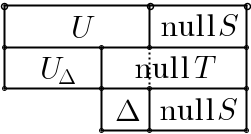
\includegraphics[width=88pt]{diagram3B-2}$}\hText{$
	\Blind{$\range S\xlongleftarrow{S}{}$}$U_{\Delta}\xlongrightarrow{T}\range T\\[-7pt]$
	$\range S\xlongleftarrow{S}\oplus\\[-6pt]$
	\Blind{$\range S\xlongleftarrow{S}{}$}$\Delta\xlongrightarrow{T}\zeroSubs}\MathLeftMid{l}{$
	Becs $\Delta=\null T\mmid_U=\null T\cap\range\BigPar{S\mmid_U}{^{-1}}.\\$
	Thus \,$E=T\BigPar{S\mmid_{U}}{^{-1}}$ is not inje $\Longleftrightarrow\Delta\neq\zeroSubs.\\$
	In other words, $\range S\mmid_\Delta=\null E,\\$
	while $E\mmid_{\cdots}:\range S\mmid_{U_\Delta}\rightarrow\range T$ is iso.$}$\par\vspace{6pt}\quad
\AComm Let $E_1\in\Lm{U_{\Delta}\oplus\null T,U_{\Delta}},$ and $E_2$ be an iso of $\range S\mmid_{U_{\Delta}}$ onto $\range T.$\parCom\quad
Define $E_1\mmid_{U_{\Delta}}=I\mmid_{U_{\Delta}},$ and $E_2=T\BigPar{S\mmid_{U_{\Delta}}}{^{-1}}.$ \;Then $T=E_2SE_1.$\par\vspace{4pt}\quad
\ACoro If $\null S=\null T.$ Then $\Delta=\zeroSubs,U_{\Delta}=U.$ \Sbra[3pt]{{\tgsl Req $W$ Finide}} \;By (3.D.3),\parCor\quad
we can extend inje $T\BigPar{S\mmid_{U}}{^{-1}}\in\Lm[\BigPar]{\range S,W}$ to inv $E\in\Lm{M,W}.$\vspace{6pt}\par\quad
\Or \Sbra[3pt]{{\tgsl Req $\range S$ Finide}} \;Let $B_{\range S}=\Par{Sv_1,\dots,Sv_n}$. Then \uline{$V=\Span{v_1,\dots,v_n}\oplus\null S$.}\par\quad
Define $E\in\Lm{\range S,W}$ by $E\Par{Sv_i}=Tv_i.$ \;Extend to $E\in\Lm{M,W}.$\par\quad
Hence $\forall v=\sum_{i=1}^na_iv_i+u\in V,\,\,$\uline{$\BigPar{\exists\,!\,u\in\null S\subseteq\null T\,},\,Tv=\sum_{i=1}^na_iTv_i+0$}${}=E\BigPar{\sum_{i=1}^na_iSv_i+0}.$\PfEnd\vspace{6pt}\quad
\ACoro \Sbra[3pt]{{\tgsl Req $W$ Finide}} \;Supp $\null S=\null T.$ We show $\exists$ inv $E\in\Lm{M,W},T=ES.$\par\quad
Redefine $E\in\Lm{M,W}$ by $E\Par{Tv_i}=Sv_i,\;E\Par{w_j}=x_j,$ for each $Tv_i$ and $w_j.$ Where:\par\quad
Let $B_{\range T}=\Par{Tv_1,\dots,Tv_m},B_W=\Par{Tv_1,\dots,Tv_m,w_1,\dots,w_n},B_U=\Par{v_1,\dots,v_m}.$\par\quad
Now $V=U\oplus\null T=U\oplus\null S\Rightarrow B_{\range S}=\BigPar{Sv_1,\dots,Sv_m}.$ Let $B_M=\Par{Sv_1,\dots,Sv_m,x_1,\dots,x_n}.$\PfEnd 
\SepLine\pagebreak

\ProblemN{\hypertarget{3B25}{25}}{
	\TextNL{Supp {\FontNorm$S\in\Lm{Y,W},T\in\Lm{V,W},$} and $\range T\subseteq\range S.$ Prove $\exists\,E\in\Lm{V,Y},T = SE$.}
}\par\quad
Let $Y=U\oplus\null S$\vspace{-4pt}\par\quad
$\Rightarrow S\mmid_U:U\rightarrow\range S$ is iso. Becs $\Par{S\mmid_U}{^{-1}}:\overset{\range T\:\subseteq}{{\range S}}\rightarrow U.$\par\quad
\uline{Define $E=\BigPar{S\mmid_U}{^{-1}}T=\BigPar{S\mmid_U}{^{-1}}\Big|{_{\range T}}T\in\Lm{V,U}\subseteq\Lm{V,Y}.$}\PfEnd\vspace{-20pt}\quad
\!\!\!$\hText{\\[6pt]$
	\AComm Let $U_1=U.$ Let $U_2\oplus\null T=V.\\$
	Let $U_{1\Delta}=\range\BigPar{S\mmid_{U_1}}{^{-1}}\Big|{_{\range T}}\subseteq U_1=\Delta\oplus U_{1\Delta}.\\$
	\Or Let $U_{1\Delta}=\range E\mmid_{U_2}.$ \,Let $\Delta\oplus\range E\mmid_{U_2}=U_1.$
%	Thus $U_1\oplus\null S=U_{1\Delta}\oplus{}$\uline{$\Par{\Delta\oplus\null S}$}${}=U_2\oplus{}$\uline{$\null T$}$.\\[-10pt]$
%	\Blind{Thus $U_1\oplus\null S=U_{1\Delta}\oplus{}$}$\qquad\text{\tiny|}\qquad\qquad\qquad\qquad\text{\tiny|}\\[-20pt]$
%	$\hspace{164.2pt}\underset{\text{iso, \;if finide.}}{\uline{\;\qquad\qquad\qquad\qquad\hspace{-2pt}}}$
$}\qquad\qquad\qquad\quad$\FontSmall$\hText{U_1\xlongrightarrow[S]{inv}\range S\\[-8pt]\;\text{\small|\:|}\qquad\qquad\text{\small|\:|}\\[-6pt]\;\Delta\,\xlongrightarrow[S]{inv}\range S\mmid_{\Delta}\\[-8pt]\;\oplus\qquad\quad\;\;\oplus\\[-6pt]\,U_{1\Delta}\xlongrightarrow[S]{inv}\range T\xlongleftarrow[T]{inv}U_2\\[-8pt]\,\;\uparrow\qquad\qquad\qquad\qquad\quad|\\[-19pt]\,\;\,\underset{inv\;\;E\def\envFontA{\normalsize}\mmid_{U_2}}{{\uline{\qquad\qquad\qquad\qquad\qquad\!\!}}}}$\FontNorm\par\vspace{2pt}\quad
%\ACoro If $\Delta=\zeroSubs,$ then $U_1=U_{1\Delta}\Rightarrow\range S=\range T.$ 又 $\null S,\null T$ are iso.\par\quad
%By (3.D.3), we can re-extend inje $E\mmid_{U_2}\in\Lm[\BigPar]{U_2,U_1\oplus\null S}$ to inv $E\in\Lm[\BigPar]{U_2\oplus\null T,U_1\oplus\null S}.$\par\vspace{4pt}\quad
%Thus we have $\Delta\neq\zeroSubs\Longleftrightarrow E\mmid_{U_2}\in\Lm{U_2,V}$ cannot be re-extended to inv $E\in\Lm{V}$ freely.
\Sbra[3pt]{{\tgsl Req $\range T$ Finide}} \;Let $B_{\range T}=\Par{Tv_1,\dots,Tv_n}.$ Now $B_{U_2}=\Par{v_1,\dots,v_n}.$\par\quad
\uline{Let $S\Par{u_i}=Tv_i$ for each $Tv_i.$} \;Define $E$ by $Ev_i=u_i,Ex=0$ for all $x\in\null T$ and each $v_i.$\PfEnd\vspace{4pt}\quad
\AComm \Sbra[3pt]{{\tgsl Req $V$ Finide}} \;Note that $\dim U_2\leqslant\dim U_1\Longrightarrow\dim\null T=p\geqslant q=\dim\null S.$\parCom\quad
Let $B_{\null T}=\Par{x_1,\dots,x_p},B_{\null S}=\Par{y_1,\dots,y_q}.$ Redefine $E:v_i\mapsto u_i,\;x_k\mapsto y_k,\;x_j\mapsto 0,$\parCom\quad
for each $i\in\Bra{1,\dots,\dim U_2},k\in\Bra{1,\dots,\dim\null S}=K,j\in\Bra{1,\dots,\dim\null T}\Backslash[\Big]K.$\parCom\quad
Note that $\Par{u_1,\dots,u_n}$ is liney indep. Let $X=\Span{x_1,\dots,x_q}\oplus\Span{v_1,\dots,v_n}.$\parCom\quad
Now $E\mmid_X$ is inje, but cannot be re-extend to inv $E\in\Lm{V,Y}$ suth $T=SE.$\par\vspace{4pt}\quad
\ACoro \Sbra[3pt]{{\tgsl Req $V$ Finide}} \;If $\range T=\range S,$ then $\dim\null T=\dim\null S=p.$\parCor\quad
Redefine $E$ by $Ev_i=u_i,\;Ex_j=y_j$ for each $v_i$ and $x_j.$ Then $E\in\Lm{V,Y}$ is inv.\PfEnd
\SepLine

\BulletPointX\AComm Supp $S,T\in\Lm{V,W}.$ Then $\range S=\range T\notRightarrow\null S,\null T$ iso.\TextB{}
\AExa Forward shift optor on $\Fbb^{\infty}$ and backward shift optor on $\Bra{\Par{0,x_1,x_2,\cdots}\in\Fbb^{\infty}}.$\TextB{\vspace{2pt}}
While $\null S=\null T\Longleftrightarrow E:Sv\mapsto Tv$ and $E^{-1}:Tv\mapsto Sv$ well-defined $\Rightarrow \range S,\range T$ iso.
\SepLine

\ProblemN{\hypertarget{3B28}{28}}{
	\TextNL{Supp $T\in\Lm{V,W}.$ Let $\Par{Tv_1,\dots,Tv_m}$ be a bss of $\range T$ and each $w_i=Tv_i.$}
	(a) \TextNL{Prove $\exists\,\varphi_1,\dots,\varphi_m\in\Lm{V,\Fbb}$ suth $\forall v\in V,Tv=\varphi_1\Par{v}w_1+\dots+\varphi_m\Par{v}w_m$.\vspace{2pt}}
	(b) {\FontSmall\Sbra{4E 3.F.5}} \TextNL{$\forall v\in V,\exists\,!\,\varphi_i\Par{v}\in\Fbb,Tv=\varphi_1\Par{v}w_1+\dots+\varphi_m\Par{v}w_m.$\vspace{1pt}}
	\Blind{(b) {\FontSmall\Sbra{4E 3.F.5}}} \TextNL{Thus defining each $\varphi_i:V\rightarrow\Fbb.$ \;Show each $\varphi_i\in\Lm{V,\Fbb}.$}
}{\FontSmall\tgsl The answer for (b) with (b) itself is the answer for (a).}\par\quad
(b) $\sum_{i=1}^m\varphi_i\Par{u+\lambda v}w_i=T\Par{u+\lambda v}=Tu+\lambda Tv={\envFontLarge\BigPar{{\envFontDefault\sum_{i=1}^m\varphi_i\Par{u}w_i}}}+\lambda{\envFontLarge\BigPar{{\envFontDefault\sum_{i=1}^m\varphi_i\Par{v}w_i}}}.$\PfEnd\vspace{4pt}\quad\Hb
\Or $\forall v\in V,\exists\,!\,a_i\in\Fbb,Tv=a_1Tv_1+\dots+a_mTv_m.$ Let $B_{\SmallPar[1pt]{\range T}\apostrophe}=\Par{\psi_1, \dots, \psi_m}$.\par\quad\Hb
Then $\Sbra{T\apostrophe\Par{\psi_{i}}}\Par{v}=\BigPar{\psi_{i}\circ T}\Par{v}=a_i.$ \,Thus each $\varphi_i=\psi_i\circ T=T\apostrophe\Par{\psi_i}\in V\apostrophe.$\PfEnd\vspace{4pt}\quad
(a) $\Span{v_1,\dots,v_m}\oplus\null T=V\Rightarrow\forall v\in V,\exists\,!\,a_i\in\Fbb,u\in\null T,\;v=\sum_{i=1}^m a_i v_i+u.$\par\quad\Ha
Define $\varphi_i\in\Lm{V,\Fbb}$ by $\varphi_i\Par{v_j}=\delta_{i,j},\;\varphi_i\Par{u}=0$ for all $u\in\null T.$\par\quad\Ha
Linity: $\forall v,w\in V\,\Sbra{\exists\,!\,a_i,b_i\in\Fbb},\lambda\in\Fbb,\varphi_i\Par{v+\lambda w}=a_i+\lambda b_i=\varphi\Par{v}+\lambda\varphi\Par{w}.$\PfEnd
\SepLine

\ProblemN{\hypertarget{3B29}{29}}{
	\TextNL{Supp $\varphi\in\Lm{V,\Fbb}.$ Supp $\varphi\Par{u}\neq 0.$ Prove $V = \null\varphi\oplus\Bra{au :a\in\Fbb}.$}\vspace{2pt}
}Let $B_{\range\varphi}=\BigPar{\varphi\Par{u}}.$ Then by \TIPSN{4}, $\Span{u}\oplus\null\varphi=V.$\PfEnd\vspace{6pt}\quad
\Or (a) $v=cu\in\null\varphi\cap\Span{u}\Rightarrow c\varphi\Par{u}=0\Rightarrow v=0.$ \;Now $\null\varphi\cap\Span{u}=\zeroSubs.$\par\vspace{5pt}\quad
\Blind{\Or}(b) $\forall\,v\in V,v=\Bigg(v-{}${\Large\envFontSmall$\frac{\varphi\Par{v}}{\varphi\Par{u}}$}$u\Bigg)+{}${\Large\envFontSmall$\frac{\varphi\Par{v}}{\varphi\Par{u}}$}$u.$ \;Now $V=\null\varphi+\Span{u}.$\PfEnd\vspace{3pt}
\SepLine\pagebreak

\ProblemN{\hypertarget{3B30}{30}}{
	\TextNL{Supp $\varphi,\beta\in\Lm{V,\Fbb}$ and $\null\varphi=\null\beta=\eta.$ Prove $\exists\,c\in\Fbb,\varphi=c\beta.$}
}If $\eta=V$, then $\varphi=\beta=0,$ done. Now by Exe (29),\par\quad
$\varphi\Par{u}\neq 0\Longleftrightarrow V=\null\varphi\oplus\Span{u}\Longleftrightarrow V=\null\beta\oplus\Span{u}\Longleftrightarrow\beta\Par{u}\neq 0.$\par\quad
\hspace{-5pt}$\hText{$
	Note that $\forall v\in V,\exists\,!\,u_0\in\eta,\;a_v\in\Fbb,v=u_0+a_vu\\$
	$\Rightarrow\varphi\Par{u_0+a_vu}=a_v\varphi\Par{u},\;\beta\Par{u_0+a_vu}=a_v\beta\Par{u}.}\;\MathLeftMid{l}{$Let $c={}${\Large\envFontSmall$\frac{\varphi\Par{u}}{\beta\Par{u}}$}${}\in\nonzeroFbb.}$\PfEnd%\vspace{6pt}
%\AComm Convly, if $\varphi=c\beta,\exists\,c\in\nonzeroFbb.$ \,Then $\null\beta=\null\Par{c\varphi}=\null\varphi.$\parCom
%Note that $c\varphi=E\circ\varphi,$ where $E\in\Lm{\Fbb}:x\rightarrow cx,$ and $E$ is inv.
\SepLine

\ProblemBnoor{\hypertarget{3F4e6}{4E 3.F.6}}{
	\TextB{Supp $\varphi,\beta\in\Lm{V,\Fbb}.$ Prove $\null \beta\subseteq\null\varphi\Longleftrightarrow\varphi=c\beta,\exists\,c\in\Fbb.$}
	\ACoro $\null \varphi=\null\beta\Longleftrightarrow\varphi=c\beta,\;\exists\,c\in\nonzeroFbb.$\TextB{}
}Using Exe (29) and (30).\par\quad
(a) If $\varphi=0,$ then done. Othws, supp $u\not\in\null\varphi\supseteq\null \beta.$\vspace{-4pt}\par\quad\Ha
Now $V=\null \varphi\oplus\Span{u}=\null \beta\oplus\Span{u}.$ By \Sbra{1.C \TIPSN{2}}, $\null \varphi=\null \beta.$ \;Let $c={}${\Large\envFontSmall$\frac{\varphi\Par{u}}{\beta\Par{u}}$}.\vspace{2pt}\par\quad\Ha
\Or We discuss in two cases. If $\null \beta=\null \varphi$, or if $\varphi=0,$ then done. Othws,\par\quad\Ha
$\exists\,u\apostrophe\in\null \varphi\Backslash[\Big]\null \beta,\,\exists\,u\not\in\null\varphi\supsetneq\null\beta\Rightarrow V=\null \beta\oplus\Span{u\apostrophe}=\null \beta\oplus\Span{u}.$\par\quad\Ha
\hspace{-5pt}$\hText{$
	$\forall v \in V, v=w+au=w\apostrophe+bu\apostrophe,\,\exists\,!\,w, w\apostrophe\in\null \beta\\$
	Thus $\varphi\Par{w+au}=a\varphi\Par{u},\,\,\beta\Par{w\apostrophe+bu}=b\beta\Par{u\apostrophe}.}\;\MathLeftMid{l}{$ Let $c={}${\Large\envFontSmall$\frac{a\varphi\Par{u}}{b\beta\Par{u\apostrophe}}$}${}\in\nonzeroFbb.$ \;Done.$}$\vspace{6pt}\par\quad\Ha
\NOTICE that by (b) below, we have $\null \varphi\subseteq\null \beta,$ ctradic the asum.\vspace{6pt}\par\quad
(b) If $c=0$, then $\null \varphi=V\supseteq\null \beta$, done. Othws, becs $v\in\null \beta\Longleftrightarrow v\in\null \varphi.$\PfEnd\vspace{4pt}\quad
\Or By Exe (24), $\null \beta\subseteq\null \varphi\Longleftrightarrow\exists\,E\in\Lm{\Fbb},\varphi=E\circ\beta.$ \Sbra{ If $E$ is inv. Then $\null \beta=\null \varphi.$ }\par\quad
Now $\exists\,E\in\Lm{\Fbb},\varphi=E\circ\beta\Longleftrightarrow\exists\,c=E\Par{1}\in\Fbb,\varphi=c\beta.$ \Sbra{ $E$ is inv $\Longleftrightarrow E\Par{1}\neq 0\Longleftrightarrow c\neq 0.$ }\PfEnd
\SepLine

\ChEnd

\vfill\ChDecl{Ch3C}{3$\cdot$C}{}\orMode{\hLk{3C1}{1}\;\;\hLk{3C3}{3}\;\;\hLk{3C4}{4}\;\;\hLk{3C5}{5}\;\;\hLk{3C6}{6}\;\;\hLk{3C9}{9}\;\;\hLk{3C10}{10}\;\;\hLk{3C11}{11}\;\;\hLk{3C13}{13}\;\;|\;\;\hLk{3C4e16}{4E:\;\;16}\;\;\hLk{3C4e17}{17}}{[1]: 10, 9, 11; [2]: (4E 16); [3]: (4E 17); [4]: 13, 1, 6; [5]: 3, 4, 5.}
\vspace{8pt}

\BulletPointX\NoteFor{[3.30, 32]}\;\;{\tgsl matrix of span}\TextB{}
Supp $L_{\alpha}=\Par{\alpha_1,\dots,\alpha_n}$ and $L_{\beta}=\Par{\beta_1,\dots,\beta_m}$ are in a vecsp $V.$\TextB{}
Let each $\alpha_k=A_{1,k}\beta_1+\dots+A_{m,k}\beta_m,$ forming $A=\Mt{\Spn L_\beta\supseteq L_{\alpha}}\in\Fbb^{m,n}.$\TextB{\vspace{3pt}}
Which is {\tgsl the matrix of span}. \;Then ${\normalsize\begin{pmatrix}\beta_1 &\hspace{-6pt} \cdots &\hspace{-6pt} \beta_m\end{pmatrix}\begin{pmatrix}
	A_{1,1} &\hspace{-6pt} \cdots &\hspace{-6pt} A_{1,n}\\[-4pt]
	\vdots	&\hspace{-6pt} \ddots &\hspace{-6pt} \vdots \\[-4pt]
	A_{m,1} &\hspace{-6pt} \cdots &\hspace{-6pt} A_{m,n}
\end{pmatrix}}={\normalsize\begin{pmatrix}\alpha_1 &\hspace{-6pt} \cdots &\hspace{-6pt} \alpha_n\end{pmatrix}}.$\TextB{\vspace{6pt}}
(a) Supp $m=n.$ If $\Par{A_{\cdot,1},\dots,A_{\cdot,n}}$ is a bss of $\Fbb^{n,1}.$ We show $L_{\alpha}$ liney indep $\Longleftrightarrow L_{\beta}$ liney indep.\TextB{}
\Ha ($\Leftarrow$) Immed. ($\Rightarrow$) Asum $L_{\beta}$ is liney dep and $\beta_j=c_1\beta_1+\dots+c_{j-1}\beta_{j-1}.$ By ctradic.\PfEnd\vspace{2pt}\TextB{}
(b) Supp $m\geqslant n.$ If $L_{\beta}$ liney indep. We show $\Par{A_{\cdot,1},\dots,A_{\cdot,n}}$ liney indep $\Longleftrightarrow L_{\alpha}$ liney indep.\TextB{}
\Hb ($\Rightarrow$) Immed. ($\Leftarrow$) By ctradic.\PfEnd\TextB{}
\Hb\AComm $\Mt{\Spn L_{\beta}\supseteq L_\alpha}=\Mt{I,L_{\alpha},L_{\beta}}\Longleftrightarrow L_{\alpha},L_{\beta}$ liney indep $\Rightarrow\Par{A_{\cdot,1},\dots,A_{\cdot,n}}$ liney indep.\parCom{\Hb\IndentB}
Where $I$ is the id optor retr to $\Spn L_{\alpha}\subseteq\Spn L_{\beta}.$
\vspace{3pt}\TextB{}
(c) Supp $m<n.$ Then $\Par{A_{\cdot,1},\dots,A_{\cdot,n}}$ is liney dep, so is $L_{\alpha}.$\TextB{\vspace{5pt}}
Supp $T\in\Lm{V,W}$ and $B_V=\Par{v_1,\dots,v_m},B_W=\Par{w_1,\dots,w_n}.$\TextB{}
Then $\Mt{T,B_V\hspace{1pt},B_W}=\Mt[\BigPar]{\Spn B_W\supseteq\Par{Tv_1,\dots,Tv_m}}.$ \; \AComm See also (4E 3.D.23).
\SepLine

\pagebreak
\def\fT{\mathcal{T}}\def\fC{\mathcal{C}}\def\fR{\mathcal{R}}\def\fP{\mathcal{E}}

\BulletPointX\NoteFor{Trspose}\;\;{\FontSmall\Sbra{\hypertarget{3F33}{3.F.33}}}\;Define $\fT:A\rightarrow A^t.$ By [3.111], $\fT$ is liney. Becs $\Par{A^t}{^t}=A.$ \TextB{}
$\fT^2=I,\,\fT=\fT^{-1}\Rightarrow \fT$ is iso of $\Fbb^{m,n}$ onto $\Fbb^{n,m}.$ \;Define $\fC_k:A\rightarrow A_{\cdot,k},\;\fR_j:A\rightarrow A_{j,\cdot},\;\fP_{j,k}:A\rightarrow A_{j,k}.$\TextB{}
%Let $A={}{\small\begin{pmatrix}1 &\hspace{-6pt} 2 &\hspace{-6pt} 3\\[-4pt] 4 &\hspace{-6pt} 5 &\hspace{-6pt} 6\end{pmatrix}}\Rightarrow A^t={}{\small\begin{pmatrix}1 &\hspace{-6pt} 4\\[-4pt] 2 &\hspace{-6pt} 5\\[-4pt] 3&\hspace{-6pt} 6\end{pmatrix}}.$ \;$\MathLeftMid{l}{$
%	\!\!$\Par{A_{2,\cdot}}{^t}={}{\small\begin{pmatrix}4 &\hspace{-6pt} 5 &\hspace{-6pt} 6\end{pmatrix}}{^t}\neq{}{\small\begin{pmatrix}2 &\hspace{-6pt} 5\end{pmatrix}}{}=\Par{A^t}{_{2,\cdot}}$ \;Simlr for all $A_{j,\cdot},A_{\cdot,k},$ and $A_{j,k}.\\[2pt]$
%	\!\!Thus in general, $\fC_k\fT\neq \fT\fC_k,\;\fR_j\fT\neq \fT\fR_j,$ \,and $\fP_{j,k}\fT\neq \fT\fP_{j,k},}$\TextB{\vspace{6pt}}
%But $\Par{A_{2,\cdot}}{^t}=\Par{A^t}{_{\cdot,2}}.$ \;
Now we show (a) \uline{$\fT\fR_j=\fC_j\fT,$} \,(b) \uline{$\fT\fC_k=\fR_k\fT,$} \,and (c) \uline{$\fT\fP_{j,k}=\fP_{k,j}\fT.$}\TextB{\vspace{2pt}}
So that $\fT\fC_k\fT=\fR_k,\;\fT\fR_j\fT=\fC_j,$ \,and $\fT\fP_{j,k}\fT=\fP_{k,j}.$\TextB{\vspace{4pt}}
Let $A={}{\normalsize\begin{pmatrix}A_{1,1} &\hspace{-6pt} \cdots &\hspace{-6pt} A_{1,n}\\[-4pt] \vdots &\hspace{-6pt} \ddots &\hspace{-6pt} \vdots\\[-4pt] A_{m,1} &\hspace{-6pt} \cdots &\hspace{-6pt} A_{m,n}\end{pmatrix}}\Rightarrow A^t={}{\normalsize\begin{pmatrix}A_{1,1} &\hspace{-6pt} \cdots &\hspace{-6pt} A_{m,1}\\[-4pt] \vdots &\hspace{-6pt} \ddots &\hspace{-6pt} \vdots\\[-4pt] A_{1,n} &\hspace{-6pt} \cdots &\hspace{-6pt} A_{m,n}\end{pmatrix}}.$ \;$\MathLeftMid{l}{\!\!$
Note that $\Par{A_{j,k}}{^t}=A_{j,k}=\Par{A^t}_{k,j}.$ Thus (c) holds.$\\$
\!\!And $\Par{A_{\cdot,k}}{^t}={}{\small\begin{pmatrix}A_{1,k} &\hspace{-6pt} \cdots &\hspace{-6pt}A_{m,k}\end{pmatrix}}{}={}{\small\begin{pmatrix}A^t_{k,1} &\hspace{-6pt} \cdots &\hspace{-6pt}A^t_{k,m}\end{pmatrix}}{}=\Par{A^t}{_{k,\cdot}}\\$
\!\!$\Longrightarrow$ (b) holds. Simlr for (a).$}$\par\vspace{8pt}
\SepLine

\BulletPointX\NoteForSmall{[3.48]}\vspace{-12pt}\par\quad
\!\!{\normalsize$\underbrace{\begin{pmatrix}
  1 &\hspace{-4pt} 2 \\[-2pt]
  3 &\hspace{-4pt} 4
\end{pmatrix}}_{A}\underbrace{\begin{pmatrix}
  5 &\hspace{-4pt} 6 &\hspace{-4pt} 7 \\[-2pt]
  8 &\hspace{-4pt} 9 &\hspace{-4pt} 10
\end{pmatrix}}_{B}{}={}\begin{pmatrix}
  \begin{pmatrix} 1 &\hspace{-4pt} 2\end{pmatrix}
  \begin{pmatrix} 5 \\[-2pt] 8\end{pmatrix}
  &\hspace{-4pt}
  \begin{pmatrix} 1 &\hspace{-4pt} 2\end{pmatrix}
  \begin{pmatrix} 6 \\[-2pt] 9\end{pmatrix}
  &\hspace{-4pt}
  \begin{pmatrix} 1 &\hspace{-4pt} 2\end{pmatrix}
  \begin{pmatrix} 7 \\[-2pt] 10\end{pmatrix}
  \\[0pt]
  \begin{pmatrix} 3 &\hspace{-4pt} 4\end{pmatrix}
  \begin{pmatrix} 5 \\[-2pt] 8\end{pmatrix}
  &\hspace{-4pt}
  \begin{pmatrix} 3 &\hspace{-4pt} 4\end{pmatrix}
  \begin{pmatrix} 6 \\[-2pt] 9\end{pmatrix}
  &\hspace{-4pt}
  \begin{pmatrix} 3 &\hspace{-4pt} 4\end{pmatrix}
  \begin{pmatrix} 7 \\[-2pt] 10\end{pmatrix}
\end{pmatrix}{}={}\begin{pmatrix} 21 &\hspace{-4pt} 24 &\hspace{-4pt} 27 \\[-2pt] 47 &\hspace{-4pt} 54 &\hspace{-4pt} 61\end{pmatrix}$}\vspace{8pt}\par
\SepLine

\BulletPointX\NoteForSmall{[3.47]}\,\, $\BigPar{AC}{_{j,k}}=\sum_{r=1}^n A_{j,r}C_{r,k}=\sum_{r=1}^n \BigPar{A_{j,\cdot}}_{1,r}\BigPar{C_{\cdot,k}}_{r,1}=\BigPar{A_{j,\cdot}C_{\cdot,k}}_{1,1}=A_{j,\cdot}C_{\cdot,k}$\PfEnd\vspace{6pt}
\BulletPointX\NoteForSmall{[3.49]} ${\envFontLarge\Sbra{\envFontDefault\BigPar{AC}_{\cdot,k}\envFontLarge}}_{j,1}=\BigPar{AC}_{j,k}=\sum_{r=1}^n A_{j,r}C_{r,k}=\sum_{r=1}^n A_{j,r}\BigPar{C_{\cdot,k}}_{r,1}=\BigPar{AC_{\cdot,k}}_{j,1}$\PfEnd\vspace{6pt}
\BulletPointX\Exercise{\hypertarget{3C10}{10}}\qquad\hspace{5pt}${\envFontLarge\Sbra{\envFontDefault\BigPar{AC}_{j,\cdot}\envFontLarge}}_{1,k}=\BigPar{AC}_{j,k}=\sum_{r=1}^n A_{j,r}C_{r,k}=\sum_{r=1}^n \BigPar{A_{j,\cdot}}_{1,r}C_{r,k}=\BigPar{A_{j,\cdot}C}_{1,k}$\PfEnd\vspace{6pt}
\BulletPointX\AComm For [3.49], let $B_U=\Par{u_1,\dots,u_p},B_V=\Par{v_1,\dots,v_n},B_W=\Par{w_1,\dots,w_m}.$\vspace{2pt}\parCom{}\IndentB{}
And $C=\Mt{T,B_U,B_V}\in\Fbb^{n,p},A=\Mt{S,B_V,B_W}\in\Fbb^{m,n}.$\vspace{1pt}\parCom{}\IndentB{}
Then $\Mt{Tu_k,B_V}=C_{\cdot,k}\Rightarrow\Mt[\BigPar]{S\Par{Tu_k},B_W}=AC_{\cdot,k}\,,$ \;又 $\Mt[\envFontLarge\BigPar]{\envFontDefault\Par{ST}\Par{u_k},B_W\envFontLarge}=\Par{AC}{_{\cdot,k}}$\PfEnd\vspace{4pt}\parCom{}\IndentB{}
By {\NOTEFOR} Transpose, $\BigPar{AC}{_{j,\cdot}}=\envFontLarge\Sbra{\BigPar{\envFontDefault\BigPar{AC}{^t}\envFontLarge}{_{\cdot,j}}}{^t}=\BigPar{C^t\Par{A^t}{_{\cdot,j}}}{^t}=\BigPar{\Par{A^t}{_{\cdot,j}}}{^t}C=A_{j,\cdot}C$\PfEnd
\SepLine

\BulletPointX\NoteForSmall{\hypertarget{3C9}{}[3.52]}\;\;$A\in\Fbb^{m,n},c\in\Fbb^{n,1}\Rightarrow Ac\in\Fbb^{m,1}.$\hfill By \Sbra{4E 3.51(a)}, $\BigPar{Ac}{_{\cdot,1}}=c_1A_{\cdot,1}+\dots+c_nA_{\cdot,n}.$\;\;\!\,\PfEnd\vspace{4pt}\quad
\Or $\because\;\BigPar{Ac}{_{j,1}}=\sum_{r=1}^n A_{j,r}c_{r,1}=\envFontLarge\Sbra{\envFontDefault\sum_{r=1}^n\BigPar{A_{\cdot,r}c_{r,1}}\envFontLarge}_{j,1}=\BigPar{c_1 A_{\cdot,1}+\dots+c_n A_{\cdot,n}}_{j,1}$\vspace{1pt}\par\quad
\Blind{\Or}$\therefore\;\,Ac=A_{\cdot,\cdot}c_{\cdot,1}=\sum_{r=1}^n A_{\cdot,r}c_{r,1}=c_1 A_{\cdot,1}+\dots+c_n A_{\cdot,n}$\;\;\Or $\BigPar{Ac}{_{j,1}}=\BigPar{Ac}{_{j,\cdot}}=A_{j,\cdot}c\in\Fbb.$\PfEnd\vspace{2pt}\quad
%$={}{\small\begin{pmatrix}A_{j,1}&\hspace{-6pt}\cdots&\hspace{-6pt}A_{j,n}\end{pmatrix}\begin{pmatrix}c_1\\[-4pt]\vdots\\[-6pt]c_n\end{pmatrix}}.$\PfEnd\vspace{-2pt}\quad
\Or Let $B_V=\Par{v_1,\dots,v_n}.$ Now $Ac=\Mt{Tv,B_W}=\Mt[\BigPar]{T\Par{c_1v_1+\dots+c_nv_n}}=c_1A_{\cdot,1}+\dots+c_nA_{\cdot,n}.$\PfEnd
%$c_1{\small\begin{pmatrix}A_{1,1}\\[-4pt]\vdots\\[-4pt]A_{m,1}\end{pmatrix}}+\dots+c_n{\small\begin{pmatrix}A_{1,n}\\[-4pt]\vdots\\[-4pt]A_{m,n}\end{pmatrix}}.$\PfEnd
\SepLine

\BulletPointX\Exercise{\hypertarget{3C11}{11}}\;\;$a\in\Fbb^{1,n},C\in\Fbb^{n,p}\Rightarrow aC\in\Fbb^{1,p}.$\hfill By \Sbra{4E 3.51(b)}, $\BigPar{aC}{_{1,\cdot}}=a_1C_{1,\cdot}+\dots+a_nC_{n,\cdot}.$\;\;\!\,\PfEnd\vspace{4pt}\quad
\Or $\because\;\BigPar{aC}{_{1,k}}=\sum_{r=1}^n a_{1,r}C_{r,k}=\envFontLarge\Sbra{\envFontDefault\sum_{r=1}^n a_{1,r}\BigPar{C_{r,\cdot}}\envFontLarge}_{1,k}=\BigPar{a_1 C_{1,\cdot}+\dots+a_n C_{n,\cdot}}_{1,k}$\vspace{2pt}\par\quad
\Blind{\Or}$\therefore\;\,aC=a_{1,\cdot}C_{\cdot,\cdot}=\sum_{r=1}^n a_{1,r}C_{r,\cdot}=a_1 C_{1,\cdot}+\dots+a_n C_{n,\cdot}$\;\;\Or $\BigPar{aC}{_{1,k}}=\BigPar{aC}{_{\cdot,k}}=aC_{\cdot,k}\in\Fbb.$\PfEnd\vspace{4pt}\quad
%$={\small\begin{pmatrix}a_1&\hspace{-6pt}\cdots&\hspace{-6pt}a_n\end{pmatrix}\begin{pmatrix}C_{1,k}\\[-4pt]\vdots\\[-4pt]C_{n,k}\end{pmatrix}}.$\PfEnd\vspace{-2pt}\quad
\Or \;$aC=\envFontLarge\BigPar{\envFontDefault\Par{aC}{^t}\envFontLarge}{^t}=\BigPar{C^ta^t}{^t}=\Sbra{a^t_1\Par{C^t}{_{\cdot,1}}+\dots+a^t_n\Par{C^t}{_{\cdot,n}}}{^t}=a_1C_{1,\cdot}+\dots+a_nC_{n,\cdot}.$\PfEnd
\SepLine

\ProblemBnoor[]{4E 3.51}[\Sbra]{
	Supp $C\in\Fbb^{m,c},R\in\Fbb^{c,p}$. \hfill\Sbra{ See also {\NOTEFOR} [3.49] and Exe (10). }\TextB{\vspace{2pt}}
	(a) For $k=1,\dots,p,$\quad $\BigPar{CR}{_{\cdot,k}}=CR_{\cdot,k}=C_{\cdot,\cdot}R_{\cdot,k}=\sum_{r=1}^c C_{\cdot,r}R_{r,k}=R_{1,k}C_{\cdot,1}+\dots+R_{c,k}C_{\cdot,c}$\TextB{\vspace{3pt}}
	%\Ha\TextB{\large Which means that each cols $CR$ is a liney combination of the cols of $C.$\vspace{6pt}}
	(b) For $j=1,\dots,m,$\quad $\BigPar{CR}{_{j,\cdot}}=C_{j,\cdot}R=C_{j,\cdot}R_{\cdot,\cdot}=\sum_{r=1}^c C_{j,r}R_{r,\cdot}=C_{j,1}R_{1,\cdot}+\dots+C_{j,c}R_{c,\cdot}$\TextB{\vspace{2pt}}
	%\Hb\TextB{\large Which means that each rows $CR$ is a liney combination of the rows of $R.$}
}\BulletPointX\AExa $m=2,c=2,p=3.$\TextB{\vspace{2pt}}
%$\BigPar{AB}_{\cdot,1}=AB_{\cdot, 1}=\begin{pmatrix} 1 &\hspace{-4pt} 2\\[-2pt] 3 &\hspace{-4pt} 4\end{pmatrix}\begin{pmatrix} 5 \\[-2pt] 8\end{pmatrix}=5\begin{pmatrix}1\\[-2pt]3\end{pmatrix}+8\begin{pmatrix}2\\[-2pt]4\end{pmatrix}=\begin{pmatrix} 21\\[-2pt] 47\end{pmatrix}$;\TextB{}
$\BigPar{AB}{_{\cdot,2}}=AB_{\cdot, 2}=\begin{pmatrix} 1 &\hspace{-4pt} 2\\[-2pt] 3 &\hspace{-4pt} 4\end{pmatrix}\begin{pmatrix} 6 \\[-2pt] 9\end{pmatrix}=A_{\cdot,1}B_{1,2}+A_{\cdot,2}B_{2,2}=6\begin{pmatrix}1\\[-2pt]3\end{pmatrix}+9\begin{pmatrix}2\\[-2pt]4\end{pmatrix}=\begin{pmatrix} 24\\[-2pt] 54\end{pmatrix}$;\TextB{\vspace{2pt}}
%$\BigPar{AB}_{\cdot,3}=AB_{\cdot, 3}=\begin{pmatrix} 1 &\hspace{-4pt} 2\\[-2pt] 3 &\hspace{-4pt} 4\end{pmatrix}\begin{pmatrix} 7 \\[-2pt] 10\end{pmatrix}=7\begin{pmatrix}1\\[-2pt]3\end{pmatrix}+10\begin{pmatrix}2\\[-2pt]4\end{pmatrix}=\begin{pmatrix} 27\\[-2pt] 61\end{pmatrix}$;\TextB{}
$\BigPar{AB}{_{1,\cdot}}=A_{1,\cdot}B=\begin{pmatrix} 1 &\hspace{-4pt} 2\end{pmatrix}\begin{pmatrix} 5 &\hspace{-4pt} 6 &\hspace{-4pt} 7 \\[-2pt] 8 &\hspace{-4pt} 9 &\hspace{-4pt} 10\end{pmatrix}=A_{1,1}B_{1,\cdot}+A_{1,2}B_{2,\cdot}=1\begin{pmatrix} 5 &\hspace{-4pt} 6 &\hspace{-4pt} 7\end{pmatrix}+2\begin{pmatrix}8 &\hspace{-4pt} 9 &\hspace{-4pt} 10\end{pmatrix}=\begin{pmatrix} 21 &\hspace{-4pt} 24 &\hspace{-4pt} 27\end{pmatrix}$;\par\vspace{6pt}
%$\BigPar{AB}_{2,\cdot}=A_{2,\cdot}B=\begin{pmatrix} 3 &\hspace{-4pt} 4\end{pmatrix}\begin{pmatrix} 5 &\hspace{-4pt} 6 &\hspace{-4pt} 7 \\[-2pt] 8 &\hspace{-4pt} 9 &\hspace{-4pt} 10\end{pmatrix}=3\begin{pmatrix} 5 &\hspace{-4pt} 6 &\hspace{-4pt} 7\end{pmatrix}+4\begin{pmatrix}8 &\hspace{-4pt} 9 &\hspace{-4pt} 10\end{pmatrix}=\begin{pmatrix} 47 &\hspace{-4pt} 54 &\hspace{-4pt} 61\end{pmatrix}$;\par
\SepLine\pagebreak

\ProblemB{
	\hspace{0pt}\textsc{\Large Column-Row Factoriz}\;\;\BigPar{CR Factoriz}\;\;\vspace{3pt}\TextB{Supp $A\in\Fbb^{m,n},A\neq 0.$}
	\TextB{Prove, with $p$ specified below, that $\exists\,C\in\Fbb^{m,p},R\in\Fbb^{p,n},A=CR.$\vspace{3pt}}
	(a) \TextB{Supp $S_c=\Span[\BigPar]{A_{\cdot,1},\cdots,A_{\cdot,n}}\subseteq\Fbb^{m,1},\dim S_c=c,\text{ the col rank}.$ Let $p=c.$\vspace{3pt}}
	(b) \TextB{Supp $S_r=\Span[\BigPar]{A_{1,\cdot},\cdots,A_{m,\cdot}}\subseteq\Fbb^{1,n},\dim S_r=r,\text{ the row rank}.$ Let $p=r.$\vspace{3pt}}
}Using [4E 3.51]. Notice that $A\neq 0\Rightarrow c,r\geqslant 1.$\vspace{2pt}\par\quad
(a) Reduce to bss $B_C=\BigPar{C_{\cdot,1},\cdots,C_{\cdot,c}},$ forming $C\in\Fbb^{m,c}$. Then $\forall k\in\Bra{1,\dots,n},$\vspace{2pt}\par\quad\Ha
$A_{\cdot,k}=R_{1,k}C_{\cdot,1}+\dots+R_{c,k}C_{\cdot,c}=\BigPar{CR}{_{\cdot,k}}\;,\exists\,!\,R_{1,k},\cdots,R_{c,k}\in\Fbb,$ forming $R\in\Fbb^{c,n}.$ Thus $A=CR.$\vspace{4pt}\par\quad
(b) Reduce to bss $B_R=\BigPar{R_{1,\cdot},\cdots,R_{r,\cdot}},$ forming $R\in\Fbb^{r,n}$. Then $\forall j\in\Bra{1,\dots,m},$\vspace{2pt}\par\quad\Hb
$A_{j,\cdot}=C_{j,1}R_{1,\cdot}+\dots+C_{j,r}R_{r,\cdot}=\BigPar{CR}{_{j,\cdot}}\;,\exists\,!\,C_{j,1},\dots,C_{j,r}\in\Fbb,$ forming $C\in\Fbb^{m,r}.$ Thus $A=CR.$\PfEnd\vspace{6pt}
\AExa $A\,=\,$ {\normalsize$\begin{pmatrix} 10 &\hspace{-4pt} 7 &\hspace{-4pt} 4 &\hspace{-4pt} 1 \\[-2pt] 26 &\hspace{-4pt} 19 &\hspace{-4pt} 12 &\hspace{-4pt} 5\\[-2pt] 46 &\hspace{-4pt} 33 &\hspace{-4pt} 20 &\hspace{-4pt} 7\end{pmatrix}$
	{$\xlongequal{\SmallPar{\text{I}}}$}
	$\begin{pmatrix} 1 &\hspace{-4pt} 0\\[-2pt] 0 &\hspace{-4pt} 1\\[-2pt] 2 &\hspace{-4pt} 1\end{pmatrix}\begin{pmatrix} 10 &\hspace{-4pt} 7 &\hspace{-4pt} 4 &\hspace{-4pt} 1\\[-2pt] 26 &\hspace{-4pt} 19 &\hspace{-4pt} 12 &\hspace{-4pt} 5\end{pmatrix}$
	{$\xlongequal{\SmallPar{\text{II}}}$}
	$\begin{pmatrix} 7 &\hspace{-4pt} 4\\[-2pt] 19 &\hspace{-4pt} 12\\[-2pt] 33 &\hspace{-4pt} 20\end{pmatrix}\begin{pmatrix} 2 &\hspace{-4pt} -1\\[-2pt] 1 &\hspace{-4pt} 0\\[-2pt] 0 &\hspace{-4pt} 1\\[-2pt] -1 &\hspace{-4pt} 2\end{pmatrix}$}\par\quad
(I) {\normalsize$\begin{pmatrix} 46 &\hspace{-4pt} 33 &\hspace{-4pt} 20 &\hspace{-4pt} 7 \end{pmatrix}=2\begin{pmatrix} 10 &\hspace{-4pt} 7 &\hspace{-4pt} 4 &\hspace{-4pt} 1\end{pmatrix}+\begin{pmatrix} 26 &\hspace{-4pt} 19 &\hspace{-4pt} 12 &\hspace{-4pt} 5\end{pmatrix}=\begin{pmatrix}2 &\hspace{-4pt} 1\end{pmatrix}\begin{pmatrix} 10 &\hspace{-4pt} 7 &\hspace{-4pt} 4 &\hspace{-4pt} 1\\[-2pt] 26 &\hspace{-4pt} 19 &\hspace{-4pt} 12 &\hspace{-4pt} 5\end{pmatrix}$}, using [4E 3.51(b)].\vspace{3pt}\par\quad\HI
{\small$\begin{pmatrix} 46 &\hspace{-4pt} 33 &\hspace{-4pt} 20 &\hspace{-4pt} 7 \end{pmatrix}$}${}\in\Span{A_{1,\cdot},A_{2,\cdot}},$ and $\Par{A_{1,\cdot},A_{2,\cdot}}$ is liney indep. Thus $B_R=\BigPar{A_{1,\cdot},A_{2,\cdot}}.$\par\vspace{6pt}\quad\EndI
(II) {\normalsize$\begin{pmatrix} 10\\[-2pt] 26\\[-2pt] 46\end{pmatrix}=2\begin{pmatrix} 7\\[-2pt] 19\\[-2pt] 33\end{pmatrix}-\begin{pmatrix} 4\\[-2pt] 12\\[-2pt] 20\end{pmatrix}; \quad \begin{pmatrix} 1\\[-2pt] 5\\[-2pt] 7\end{pmatrix}=-\begin{pmatrix} 7\\[-2pt] 19\\[-2pt] 33\end{pmatrix}+2\begin{pmatrix} 4\\[-2pt] 12\\[-2pt] 20\end{pmatrix}$}. \;Thus $B_C=\BigPar{A_{\cdot,2},A_{\cdot,3}}.$\vspace{6pt}\par
\SepLine

\BulletPointX\textsc{Column Rank Equals Row Rank}\quad Using nota and result above.\TextB{}
For each $A_{j,\cdot}\in S_r,\;A_{j,\cdot}=\BigPar{CR}{_{j,\cdot}}=C_{j,\cdot}R=C_{j,1}R_{1,\cdot}+\dots+C_{j,c}R_{c,\cdot}$\TextB{}
For each $A_{\cdot,k}\in S_c,\;A_{\cdot,k}=\BigPar{CR}{_{\cdot,k}}=CR_{\cdot,k}=R_{1,k}C_{\cdot,1}+\dots+R_{c,k}C_{\cdot,c}$\TextB{}
$\Rightarrow\Span[\BigPar]{A_{1,\cdot},\cdots,A_{n,\cdot}}=S_r=\Span[\BigPar]{R_{1,\cdot},\cdots,R_{c,\cdot}}\Rightarrow\dim S_r=r\leqslant c=\dim S_c.$\TextB{}
$\Rightarrow\Span[\BigPar]{A_{\cdot,1},\cdots,A_{\cdot,m}}=S_c=\Span[\BigPar]{C_{\cdot,1},\cdots,C_{\cdot,r}}\Rightarrow\dim S_c=c\leqslant r=\dim S_r.$\TextB{}
\Or Apply the result to $A^t\in\Fbb^{n,m}\Rightarrow\dim S_r^t=\dim S_c=c\leqslant r=\dim S_r=\dim S_c^t.$\PfEnd
\SepLine

\def\rank{{\textup{\tgnr rank}}\,}

\ProblemB{
	\hypertarget{3C4e16}{}\TextB{Supp $A\in\Fbb^{m,n}\nonzero.$ Prove [P] $\rank A=1\Longleftrightarrow\exists\,c_j,d_k\in\Fbb,$ each $A_{j,k}=c_j\cdot d_k.$ [Q]}
}\par\quad
\!\Sbra[3pt]{{\tgsl Using CR Factoriz}}\par\quad
$P\Rightarrow Q:$ \;Immed.\par\vspace{-12pt}\quad
$Q\Rightarrow P:$ \;Becs $\;A={}${\normalsize$\begin{pmatrix}c_1 \\[-4pt] \vdots \\[-5pt] c_m \end{pmatrix}\begin{pmatrix}d_1 & \hspace{-6pt}\cdots & \hspace{-6pt}d_n\end{pmatrix}$}${}={}${\normalsize$\begin{pmatrix} c_1 d_1 & \hspace{-6pt}\cdots & \hspace{-6pt}c_1 d_n\\[-4pt] \vdots & \hspace{-6pt}\ddots & \hspace{-6pt}\vdots \\[-5pt] c_m d_1 & \hspace{-6pt}\cdots & \hspace{-6pt}c_m d_n \end{pmatrix}$} $\Longrightarrow S_r=\Spn${\FontSmall$\MathLeftrightBrace{l}{
	\!\begin{pmatrix}\uline{c_1} d_1 & \hspace{-6pt}\cdots & \hspace{-6pt}\uline{c_1} d_n\end{pmatrix},\\[-6pt] \;\;\;\qquad\vdots\\[-6pt]
	\!\begin{pmatrix}\uline{c_m} d_1 & \hspace{-6pt}\cdots & \hspace{-6pt}\uline{c_m} d_n\end{pmatrix}
}%=\Spn\!\MathLeftrightBrace{c}{\!\!\begin{pmatrix}d_1 & \hspace{-6pt}\cdots & \hspace{-6pt}d_n\end{pmatrix}\!\!\!}
$}.\par\vspace{0pt}\quad
\Blind{$Q\Rightarrow P:$ \;}\Or $S_c=\Spn${\normalsize$\MathLeftrightBrace{c}{\!\!\begin{pmatrix} c_1\uline{d_1} \\[-4pt] \vdots \\[-5pt] c_m\uline{d_1}\end{pmatrix},\dots,\begin{pmatrix} c_1\uline{d_n} \\[-4pt] \vdots \\[-5pt] c_m\uline{d_n}\end{pmatrix}\!\!\!}$}${}={}\Spn${\normalsize$\MathLeftrightBrace{c}{\!\!\begin{pmatrix}c_1 \\[-4pt] \vdots \\[-5pt] c_m\end{pmatrix}\!\!\!}$}.\PfEnd\vspace{12pt}\quad
%$\exists\,C={}${\normalsize$\begin{pmatrix}c_1 \\[-4pt] \vdots \\[-5pt] c_m \end{pmatrix}$}${}\in\Fbb^{m,1},R=\begin{pmatrix} d_1 & \hspace{-6pt}\cdots & \hspace{-6pt}d_n\end{pmatrix}\in\Fbb^{1,n}$ suth $A=CR.$
\!\Sbra[3pt]{{\tgsl Not Using CR Factoriz}}\vspace{-8pt}\par\quad
$Q\Rightarrow P:$\,\;Using [4E 3.51(a)]. Each $A_{\cdot,k}\in\Spn${\normalsize$\MathLeftrightBrace{c}{\!\!\begin{pmatrix}c_1 \\[-4pt] \vdots \\[-5pt] c_m\end{pmatrix}\!\!\!}$}. $\hText{$
	Then $\rank A=\dim S_c\leqslant 1\\$
	又 $A\neq 0\Rightarrow\dim S_c\geqslant 1.}$\vspace{-8pt}\par\quad
$P\Rightarrow Q:$\,\;Becs $\dim S_c=\dim S_r=1.$\vspace{4pt}\par\quad
\Blind{$P\Rightarrow Q:$\,\;}{\vspace{8pt}Let $c_j=\Frac{A_{j,1}}{A_{1,1}}=\Frac{A_{j,2}}{A_{1,2}}=\dots=\Frac{A_{j,n}}{A_{1,n}},\quad d_k'=\Frac{A_{1,k}}{A_{1,1}}=\Frac{A_{2,k}}{A_{2,1}}=\dots=\Frac{A_{m,k}}{A_{m,1}}.$}\par\quad
\Blind{$P\Rightarrow Q:$\,\;}{$\Rightarrow A_{j,k}=d_k' A_{j,1}=c_j A_{1,k}=c_j d_k' A_{1,1}=c_j d_k,$ where $d_k=d_k' A_{1,1}.$}\PfEnd
\SepLine\pagebreak

%Note that $T$ is inveritlbe $\Longleftrightarrow$ $T\apostrophe$ is inv. And $A^t=\Mt{T\apostrophe,B_{\beta}\apostrophe,B_{\alpha}\apostrophe}.$\par\quad
%(a) Supp $T$ is inv, so is $T\apostrophe$. Becs $\BigPar{T\apostrophe\Par{\varphi_1},\dots,T\apostrophe\Par{\varphi_m}}$ is liney indep.\par\quad\Ha
%\NOTICE that $T\apostrophe\Par{\varphi_i}=A^t_{1,i}\psi_1+\dots+A^t_{m,i}\psi_m.$ By the \Par{$\Delta$} part in (4E 3.C.17),\par\quad\Ha
%the cols of $A^t$, namely the rows of $A$, are liney indep.\par\quad
%(b) Supp the rows of $A$ are liney indep, so are the cols of $A^t$. \NOTICE that $A^t$ has $\dim V\apostrophe$ cols.
%Then $B_{\range T\apostrophe}=B_{V\apostrophe}=\BigPar{T\apostrophe\Par{\varphi_1},\dots,T\apostrophe\Par{\varphi_m}}.$ Thus $T\apostrophe$ is surj. Hence $T\apostrophe$ is inv, so is $T.$\par

\ProblemB{
	\TipsN{1}\,\,\,\TextB{Supp $T\in\Lm{V,W},\;B_V=\Par{v_1,\dots,v_n},B_W=\Par{w_1,\dots,w_m}.$\vspace{-1pt}}
	\IndentTipsN{1}{\tgsl Let $L=\BigPar{Tv_{\alpha_1},\dots,Tv_{\alpha_k}},\;L_{\mathcal{M}}=\BigPar{A_{\cdot,\alpha_1},\cdots,A_{\cdot,\alpha_k}},$ where each $\alpha_i\in\Bra{1,\dots,n}.$}\TextB{\vspace{1pt}}
	\IndentTipsN{1}(a) \TextB{Show [P] $L$ is liney indep $\Longleftrightarrow L_{\mathcal{M}}$ is liney indep. [Q]\vspace{2pt}}
	\IndentTipsN{1}(b) \TextB{Show [P] $\Spn L=W\Longleftrightarrow\Spn L_{\mathcal{M}}=\Fbb^{m,1}.$ [Q]\hfill\FontNorm\Sbra{ Let $A=\Mt{T,B_V,B_W}.$\hspace{1pt}}\vspace{3pt}}
}(a) Note that $\mathcal{M}\!:\,Tv_k\rightarrow A_{\cdot,k}$ is iso. of $\Spn L$ onto $\Spn L_{\mathcal{M}}.$ By (3.B.9).\parSol{}
(b) Reduce to liney indep lists. By (a) and (2.39).\PfEnd\vspace{4pt}\quad
\Or\;$c_1Tv_{\alpha_1}+\dots+c_kTv_{\alpha_k}=c_1\BigPar{A_{1,{\alpha_1}}w_1+\dots+A_{m,{\alpha_1}}w_m}+\dots+c_k\BigPar{A_{1,{\alpha_k}}w_1+\dots+A_{m,{\alpha_k}}w_m}$\par\vspace{2pt}\quad
\Blind{\Or\;}$\Blind{c_1Tv_{\alpha_1}+\dots+c_kTv_{\alpha_k}}=\BigPar{c_1A_{1,{\alpha_1}}+\dots+c_kA_{1,{\alpha_k}}}w_1+\dots+\BigPar{c_1A_{m,{\alpha_1}}+\dots+c_kA_{m,{\alpha_k}}}w_m.$\par\vspace{4pt}\quad
\Blind{\Or\;}And \;$c_1A_{\cdot,{\alpha_1}}+\dots+c_kA_{\cdot,{\alpha_k}}=c_1{\normalsize\begin{pmatrix}A_{1,{\alpha_1}}\\[-4pt]\vdots\\[-10pt]A_{m,{\alpha_1}}\end{pmatrix}}+\dots+c_k{\normalsize\begin{pmatrix}A_{1,{\alpha_k}}\\[-4pt]\vdots\\[-10pt]A_{m,{\alpha_k}}\end{pmatrix}}{}={}\normalsize\begin{pmatrix}c_1 A_{1,{\alpha_1}}+\dots+c_kA_{1,{\alpha_k}}\\[-4pt]\vdots\\[-4pt]c_1A_{m,{\alpha_1}}+\dots+c_kA_{m,{\alpha_k}}\end{pmatrix}$.\par\vspace{6pt}\quad
(a) $P\Rightarrow Q:$\,\;Supp $\;c_1A_{\cdot,{\alpha_1}}+\dots+c_kA_{\cdot,{\alpha_k}}=0.$ \;Let $v=c_1v_{\alpha_1}+\dots+c_kv_{\alpha_k}.$\par\quad\Ha
\Blind{$Q\Rightarrow P:$\,\;}Then $Tv=\BigPar{c_1A_{1,{\alpha_1}}+\dots+c_kA_{1,{\alpha_k}}}w_1+\dots+\BigPar{c_1A_{m,{\alpha_1}}+\dots+c_kA_{m,{\alpha_k}}}w_m=0w_1+\dots+0w_m.$\par\quad\Ha
\Blind{$Q\Rightarrow P:$\,\;}Now $c_1Tv_{\alpha_1}+\dots+c_kTv_{\alpha_k}=0.$ Then each $c_i=0\Rightarrow L_{\mathcal{M}}$ liney indep.\vspace{4pt}\par\quad\Ha
$Q\Rightarrow P:$\,\;Becs $c_1Tv_{\alpha_1}+\dots+c_kTv_{\alpha_k}=0.$ For each $i\in\Bra{1,\dots,m},\;c_1A_{i,{\alpha_1}}+\dots+c_kA_{i,{\alpha_k}}=0.$\par\quad\Ha
\Blind{$Q\Rightarrow P:$\,\;}Which is equiv to $c_1A_{\cdot,{\alpha_1}}+\dots+c_kA_{\cdot,{\alpha_k}}=0.$ \;Thus each $c_i=0\Rightarrow L$ liney indep.\par\vspace{4pt}\quad\Ha
\Or\;$\exists\,A_{\cdot,{\alpha_j}}=c_1A_{\cdot,{\alpha_1}}+\dots+c_{j-1}A_{\cdot,{\alpha_{j-1}}}$\par\quad\Ha
\Blind{\Or\;}$\Longleftrightarrow$ For each $i\in\Bra{1,\dots,m},\;A_{i,{\alpha_j}}=c_1A_{i,{\alpha_1}}+\dots+c_{j-1}A_{i,{\alpha_{j-1}}}$\par\quad\Ha
\Blind{\Or\;}$\Longleftrightarrow Tv_{\alpha_j}=A_{1,{\alpha_j}}w_1+\dots+A_{m,{\alpha_j}}w_m$\par\vspace{2pt}\quad\Ha
\Blind{\Or\;}$\Blind{\Longleftrightarrow Tv_{\alpha_j}}=\BigPar{c_1A_{1,{\alpha_1}}+\dots+c_{j-1}A_{1,{\alpha_{j-1}}}}w_1+\dots+\BigPar{c_1A_{m,{\alpha_1}}+\dots+c_{j-1}A_{m,{\alpha_{j-1}}}}w_m$\par\vspace{2pt}\quad\Ha
%\Blind{\Or}$\Blind{\Longleftrightarrow Tv_{\alpha_j}}=c_1\BigPar{A_{1,\alpha_1}w_1+\dots+A_{m,\alpha_1}w_m}+\dots+c_{j-1}\BigPar{A_{1,\alpha_{j-1}}w_1+\dots+A_{m,\alpha_{j-1}w_m}}$\par\quad\Ha
\Blind{\Or\;}$\Longleftrightarrow\exists\,Tv_{\alpha_j}=c_1Tv_{\alpha_1}+\dots+c_{j-1}Tv_{\alpha_{j-1}}.$\par\vspace{6pt}\quad
(b) Note that each $\Mt{Tv_{\alpha_i}}=A_{\cdot,\alpha_i}$\par\quad\Hb
$P\Rightarrow Q:$\,\;Supp each $w_i=Iw_i=J_{1,i}Tv_{\alpha_1}+\dots+J_{k,i}Tv_{\alpha_k}.$\par\quad\Hb
%Then fix one $J=\Mt{I,B_W,L}\in\Fbb^{k,m}.$
\Blind{$Q\Rightarrow P:$\,\;}$\forall a\in\Fbb^{m,1},\exists\,w=a_1w_1+\dots+a_mw_m\in W,\;a=\Mt{w,B_W}.$\par\quad\Hb
\Blind{$Q\Rightarrow P:$\,\;}Becs $w=a_1\BigPar{J_{1,1}Tv_{\alpha_1}+\dots+J_{k,1}Tv_{\alpha_k}}+\dots+a_m\BigPar{J_{1,m}Tv_{\alpha_1}+\dots+J_{k,m}Tv_{\alpha_k}}$\par\vspace{2pt}\quad\Hb
\Blind{$Q\Rightarrow P:$\,\;Becs} $\Blind{w}=\BigPar{a_1J_{1,1}+\dots+a_mJ_{1,m}}Tv_{\alpha_1}+\dots+\BigPar{a_1J_{k,1}+\dots+a_mJ_{k,m}}Tv_{\alpha_k}.$\par\vspace{2pt}\quad\Hb
\Blind{$Q\Rightarrow P:$\,\;}Apply $\mathcal{M}$ to both sides, $a=c_1A_{\cdot,\alpha_1}+\dots+c_kA_{\cdot,\alpha_k},$ where each $c_i=a_1J_{i,1}+\dots+a_mJ_{i,m}.$\par\vspace{6pt}\quad\Hb
$Q\Rightarrow P:$\,\;$\forall w\in W,\exists\,a=c_1A_{\cdot,{\alpha_1}}+\dots+c_kA_{\cdot,\alpha_k}\in\Fbb^{m,1},\;\Mt{w,B_W}=a$\par\quad\Hb
\Blind{$Q\Rightarrow P:$\,\;}$\Rightarrow w=\BigPar{c_1A_{1,{\alpha_1}}+\dots+c_kA_{1,{\alpha_k}}}w_1+\dots+\BigPar{c_1A_{m,{\alpha_1}}+\dots+c_kA_{m,{\alpha_k}}}w_m=c_1Tv_{\alpha_1}+\dots+c_kTv_{\alpha_k}.$\vspace{6pt}\par\quad\Hb
${}{^\neg}Q\Rightarrow{}{^\neg}P:$\,\;$\exists\,w\in W,\exists\,a\in\Fbb^{m,1},\Mt{w,B_W}=a,$ but $\nexists\,\Par{c_1,\dots,c_k}\in\Fbb^k,a=c_1A_{\cdot,\alpha_1}+\dots+c_kA_{\cdot,\alpha_k}$\par\quad\Hb
\Blind{${}{^\neg}Q\Rightarrow{}{^\neg}P:$\,\;}$\Rightarrow\nexists\,\Par{c_1,\dots,c_k}\in\Fbb^k,\;w=c_1Tv_{\alpha_1}+\dots+c_kTv_{\alpha_k}.$ For if not, ctradic.\PfEnd\vspace{6pt}
\Note \,\,\,Let $L=\BigPar{Tv_1,\dots,Tv_n},\;L_{\mathcal{M}}=\BigPar{A_{\cdot,1},\cdots,A_{\cdot,n}}.$\parNot
Then (a*) By \Sbra{3.B.9, \TIPSN{4}}, $T$ is inje $\Longleftrightarrow L$ is liney indep, so is $L_{\mathcal{M}}$.\parNot
And (b*) $T$ is surj $\Longleftrightarrow\Spn L=W\Longleftrightarrow\Spn L_{\mathcal{M}}=\Fbb^{m,1}.$\parNot
\hypertarget{3C4e17}{\ACoro }$B_{\Fbb^{n,1}}=\BigPar{A_{\cdot,1},\cdots,A_{\cdot,n}}\Longleftrightarrow T$ is inje and surj $\Longleftrightarrow B_{\Fbb^{1,n}}=\BigPar{A_{\cdot,1},\cdots,A_{\cdot,n}}.$\parNot
\AComm If $T$ is inv. Then by (a*, c) or (b*, d), we have another proof of \COROLLARY.\parNot\IndentComment
\hypertarget{3F32}{\Or }If $m=n.$ Then by [3.118] and one of (a*, b*, c, d). Yet another proof.\parNot
(c) $T$ surj $\Longleftrightarrow T\apostrophe$ inje $\Longleftrightarrow\BigPar{T\apostrophe\Par{\psi_1},\dots,T\apostrophe\Par{\psi_m}}$ liney indep\parNot\Hc
\Blind{$T$ surj }$\xLongleftrightarrow{\text{(a)}}{\envFontLarge\BigPar{{\envFontDefault\Par{A^t}{_{\cdot,1}},\cdots,\Par{A^t}{_{\cdot,m}}}}}$ liney indep in $\Fbb^{n,1},$ so is $\BigPar{A_{1,\cdot},\cdots,A_{m,\cdot}}$ in $\Fbb^{1,n}.$\vspace{4pt}\parNot
(d) $T$ inje $\Longleftrightarrow T\apostrophe$ surj $\Longleftrightarrow V\apostrophe=\Span[\BigPar]{T\apostrophe\Par{\psi_1},\dots,T\apostrophe\Par{\psi_m}}$\parNot\Hd
\Blind{$T$ inje }$\xLongleftrightarrow{\text{(b)}}\Fbb^{n,1}=\Span[\envFontLarge\BigPar]{{\envFontDefault\Par{A^t}{_{\cdot,1}},\cdots,\Par{A^t}{_{\cdot,m}}}}\Longleftrightarrow\Fbb^{1,n}=\Span[\envFontLarge\BigPar]{A_{1,\cdot},\cdots,A_{m,\cdot}}.$
\SepLine

\ProblemB{
	\TipsN{2}\,\,\,\TextB{Supp $p$ is a poly of $\,n\,$ variables in $\Fbb.$ Prove $\Mt[\BigPar]{p\Par{T_1,\dots,T_n}}=p\BigPar{\Mt{T_1},\dots,\Mt{T_n}}.$}
	\IndentTipsN{2}\TextB{\FontNorm Where the liney maps $T_1,\dots,T_n$ are suth $p\Par{T_1,\dots,T_n}$ makes sense. \tgnr See [5.16,17,20].}
}Supp the poly $p$ is defined by $p\Par{x_1,\dots,x_n}=\sum_{k_1,\dots,k_n}\!\!\alpha_{k_1,\dots,k_n}\prod_{i=1}^n x_i^{k_i}.$\parSol{\vspace{4pt}}
Note that $\Mt{T^x S^y}=\Mt{T}{^x}\Mt{S}{^y};\;\Mt{T^x+S^y}=\Mt{T}{^x}+\Mt{S}{^y}.$\parSol{\vspace{4pt}}
Then $\Mt[\BigPar]{ p\Par{T_1,\dots,T_n}}={\Mt[\envFontLarge\BigPar]{{\envFontDefault\sum_{k_1,\dots,k_n}\!\!\alpha_{k_1,\dots,k_n}\prod_{i=1}^n T_i^{k_i}}}}$\parSol{\vspace{4pt}}
\Blind{Then $\Mt[\BigPar]{ p\Par{T_1,\dots,T_n}}$} $={\sum_{k_1,\dots,k_n}\!\!\alpha_{k_1,\dots,k_n}\prod_{i=1}^n\Mt[\BigPar]{T_i^{k_i}}}={p\envFontLarge\BigPar{{\envFontDefault\Mt{T_1},\dots,\Mt{T_n}}}}.$\PfEnd\vspace{6pt}
\BulletPointX\ACoro Supp $\tau$ is an algebraic property. Then $\tau$ holds for liney maps $\Longleftrightarrow \tau$ holds for matrices.\parCor{\IndentB}
Supp $\alpha_1,\dots,\alpha_n$ are dist with each $\alpha_k\in\Bra{1,\dots,n}.$\parCor{\IndentB}
Now $p\Par{T_1,\dots,T_n}=p\Par{T_{\alpha_1},\dots,T_{\alpha_n}}\Longleftrightarrow p\envFontLarge\BigPar{{\envFontDefault\Mt{T_1},\dots,\Mt{T_n}}}=p\BigPar{{\envFontDefault\Mt{T_{\alpha_1}},\dots,\Mt{T_{\alpha_n}}}}.$\SepLine

\ProblemN{\hypertarget{3C13}{13}}{
	\TextNL{Prove the distr holds for matrix add and matrix multi.}
	\TextNL{\FontNorm Supp $A, B, C$ are matrices suth $A\Par{B + C}$ make sense, we prove the left distr.}
}Supp $A\in\Fbb^{m,n}$ and $B,C\in\Fbb^{n,p}.$\parSol{}
Note that ${\envFontLarge\Sbra{{\envFontDefault A\BigPar{B+C}}}}{_{j,k}}=\sum_{r=1}^n A_{j,r}\BigPar{B+C}{_{r,k}}=\sum_{r=1}^n \BigPar{A_{j,r}B_{r,k}+A_{j,r}C_{r,k}}=\BigPar{AB+AC}{_{j,k}}.$\parSol{\vspace{6pt}}
\Or Define $T,S,R$ suth $\Mt{T}=A,\Mt{S}=B,\Mt{R}=C.$\parSol{}
$A\Par{B+C}=\Mt{T\Par{S+R}}\xlongequal{\text{[3.9]}}\Mt{TS+TR}=AB+AC.$\parSol{}
\Or $T\Par{S+R}=TS+TR\Rightarrow\Mt{T\Par{S+R}}=\Mt{TS+TR}\Rightarrow A\Par{B+C}=AB+AC.$\PfEnd
\SepLine

%\ProblemN{\hypertarget{3C14}{14}}{
	%	\TextNL{Prove matrix multi is associ.}
	%	\TextNL{\FontNorm Supp $A,B,C$ are matrices suth $\Par{AB}C$ makes sense, we prove $\Par{AB}C=A\Par{BC}.$}
	%}Supp $A\in\Fbb^{m,n}$ and $B,C\in\Fbb^{n,p}.$ We show $LHS=\Sbra{\Par{AB}C}_{j,k}=\Sbra{A\Par{BC}}_{j,k}=RHS.$\parSol{}
%$LHS=\BigPar{AB}{_{j,\cdot}}C_{\cdot,k}=\sum_{s=1}^n\BigPar{A_{j,s}B_{s,\cdot}}C_{\cdot,k}=\sum_{s=1}^n A_{j,s}\BigPar{B_{s,\cdot}C_{\cdot,k}}=\sum_{s=1}^n A_{j,s}\BigPar{BC}{_{s,k}}=RHS.$\PfEnd\parSol{\vspace{6pt}}
%\Or Define $T,S,R$ suth $\Mt{T}=A,\Mt{S}=B,\Mt{R}=C.$\parSol{}
%$\Par{AB}C=\Mt{T\Par{SR}}\xlongequal{\text{[3.9]}}\Mt{TSR}\xlongequal{\text{[3.9]}}\Mt{\Par{TS}R}=A\Par{BC}.$\parSol{}
%\Or $\Par{TS}R=T\Par{SR}\Rightarrow\Mt{\Par{TS}R}=\Mt{T\Par{SR}}\Rightarrow \Par{AB}C=A\Par{BC}.$\PfEnd
%\SepLine

%\ProblemN{\hypertarget{3C15}{15}}{
	%	\TextNL{Supp $A\in\Fbb^{n,n},j,k\in\Bra{1,\dots,n}$. Show $\BigPar{A^3}_{j,k}=\sum_{p=1}^n \sum_{r=1}^n A_{j,p}A_{p,r}A_{r,k}$.\vspace{6pt}}
	%}\vspace{-6pt}\AlignEq{}{\BigPar{AAA}_{j,k} &= \BigPar{AA}_{j,\cdot}\hspace{1pt}A_{\cdot,k}=\textstyle\sum_{p=1}^n \BigPar{A_{j,p}A_{p,\cdot}}A_{\cdot,k}=\textstyle\sum_{p=1}^n \sum_{r=1}^n A_{j,p}A_{p,r}A_{r,k}.\hspace{60pt}\\
	%	\text{\Or}\;\;\BigPar{AAA}_{j,k} &=\textstyle\sum_{r=1}^n\BigPar{AA}_{j,r}A_{r,k} =\textstyle\sum_{r=1}^n\XPar{\sum_{p=1}^n A_{j,p}A_{p,r}}\hspace{1pt}A_{r,k}\\&=\uline{\textstyle\sum_{r=1}^n\left[A_{j,1}\BigPar{A_{1,r}A_{r,k}}+\dots+A_{j,n}\BigPar{A_{n,r}A_{r,k}}\right]}\\&=\textstyle A_{j,1}\sum_{r=1}^n A_{1,r}A_{r,k}+\dots+A_{j,n}\textstyle\sum_{r=1}^n A_{n,r}A_{r,k}=\textstyle\sum_{p=1}^n \sum_{r=1}^n A_{j,p}A_{p,r}A_{r,k}.}\PfEnd[-25pt]
%\SepLine

%\ProblemB{
	%	\hypertarget{3C12}{}\TextB{Prove the commu does not hold in $\Fbb^{m,n}.$}
	%}Supp $\dim V=n,\dim W=m$ and the commu holds in $\Fbb^{n,m}.$\parSol{}
%$\forall T\in\Lm{V,W},S\in\Lm{W,V},\Mt{TS}=\Mt{T}\Mt{S}=\Mt{S}\Mt{T}=\Mt{ST}.$\parSol{}
%Hence $ST=TS.$ Which in general does not hold.\PfEnd
%\SepLine

%\ProblemN{12}{
	%	\TextNL{Give an exa of 2-by-2 matrices $A$ and $B$ suth $AB\neq BA$.}\vspace{6pt}
	%}$\begin{pmatrix} 1 & 0\\ 0 & -1\end{pmatrix}\begin{pmatrix}
	%0 & 1\\ 1 & 0\end{pmatrix}=\begin{pmatrix} 0 & 1\\ -1 & 0\end{pmatrix};$\qquad
%$\begin{pmatrix} 0 & 1\\ 1 & 0\end{pmatrix}\begin{pmatrix}
	%1 & 0\\ 0 & -1\end{pmatrix}=\begin{pmatrix} 0 & -1\\ 1 & 0\end{pmatrix}.$\vspace{6pt}\par
%\SepLine

\ProblemN{\hypertarget{3C1}{1}}{
	\TextN{Supp $T\in\Lm{V,W}.$ Show for each pair of $B_V$ and $B_W,$}
	\TextN{$A=\Mt{T,B_V,B_W}$ has at least $n=\dim\range T$ nonzero ent.}
}\par\quad
Let $U\oplus\null T=V;\;B_U=\Par{v_1,\dots,v_n},B_V=\Par{v_1,\dots,v_m}.$\par\quad
For each $k\in\Bra{1,\dots,n},Tv_k\neq 0\Longleftrightarrow A_{\cdot,k}\neq 0.$ Hence every such $A_{\cdot,k}$ has at least one nonzero ent.\PfEnd\vspace{4pt}\par\quad
\Or We prove by ctradic. Supp $A$ has at most $\Par{n-1}$ nonzero ent.\par\quad
Then by Pigeon Hole Principle, at least one of $A_{\cdot,1},\dots,A_{\cdot,n}$ equals $0$.\par\quad
Thus there are at most $\Par{n-1}$ nonzero vecs in $Tv_{1},\dots,Tv_n.$\par\quad
又 $\range T=\Span{Tv_{1},\dots,Tv_n}\Rightarrow\dim\range T=\dim\Span{Tv_{1},\dots,Tv_n}\leqslant n-1.$ Ctradic.\PfEnd
\SepLine

\ProblemN{\hypertarget{3C6}{6}}{
	\TextN{Supp $V$ and $W$ are finide and $T\in\Lm{V,W}$.}
	\TextN{Prove $\dim\range T = 1\Longleftrightarrow\exists\,B_V,B_W,$ all ent of $A=\Mt[\BigPar]{T,B_V,B_W}$ equal $1$.}
}\par\quad
(a) Supp $B_V=\Par{v_1,\dots,v_n},B_W=\Par{w_1,\dots,w_m}$ are the bses suth all ent of $A$ equal $1$.\par\quad\Ha
Then $Tv_i=w_1+\dots+w_m$ for all $i=1,\dots,n$. Becs $w_1,\dots,w_n$ is liney indep, $w_1+\dots+w_n\neq 0.$\vspace{4pt}\par\quad
(b) Supp $\dim\range T=1$. Then $\dim\null T=\dim V-1$.\par\quad\Hb
Let $B_{\null T}=\Par{u_2,\dots,u_n}.$ Extend to a bss $\Par{u_1,u_2,\dots,u_n}$ of $V.$\par\quad\Hb
Becs $Tv_1\neq 0.$ Extend to $\Par{Tv_1,w_2,\dots,w_m}$ a bss of $W.$ Let $w_1=Tv_1-w_2-\dots-w_m.$\par\quad\Hb
Now $B_W=\Par{w_1,\dots,w_m}.$ \;Let \,$v_1=u_1,\;v_i=u_1+u_i.$ \,Now $B_V=\Par{v_1,\dots,v_n}.$\PfEnd\vspace{6pt}\quad\Hb
\Or Supp $B_{\range T}=\Par{w}.$ \,By \Sbra{2.C {\NOTEFOR} (15)}, $\exists\,B_W=\Par{w_1,\dots,w_m},\;w=w_1+\dots+w_m.$\par\quad\Hb
By \Sbra{2.C {\TIPS}}, $\exists$ a bss $\Par{u_1,\dots,u_n}$ of $V$ suth each $u_k\not\in\null T.$\par\quad\Hb
Now each $Tu_k\in\range T=\Span{w}\Rightarrow Tu_k=\lambda_k w,\exists\,\lambda_k\in\nonzeroFbb.$\par\quad\Hb
Let $v_k=\lambda_k^{-1}u_k\neq 0,$ so that each $Tv_k=w=w_1+\dots+w_m.$ Thus $B_V=\Par{v_1,\dots,v_n}$ will do.\PfEnd
\SepLine\pagebreak

\ProblemN{\hypertarget{3C3}{3}}{
	\TextN{Supp $V$ and $W$ are finide and $T\in\Lm{V,W}$. Prove $\exists\,B_V,B_W$ suth}
	\TextN{[ letting $A=\Mt{T,B_V,B_W}$ ] $A_{k,k}=1,A_{i,j}=0$, where $1\leqslant k\leqslant \dim\range T, i\neq j$.\vspace{2pt}}
}Let $B_{\null T}=\Par{u_1,\dots,u_m},B_{\range T}=\Par{Tv_1,\dots,Tv_n}\Rightarrow B_V=\BigPar{v_1,\dots,v_n,u_1,\dots,u_m}.$\PfEnd\vspace{2pt}
\AComm Let each $Tv_k=w_k.$ Extend $B_{\range T}$ to $B_W=\BigPar{w_1,\dots,w_n,\dots,w_p}.$ See \Sbra{3.D {\NOTEFOR} [3.60]}.
\SepLine

\ProblemN{\hypertarget{3C4}{4}}{
	\TextN{Supp $B_V=\Par{v_1,\dots,v_m}$ and $W$ is finide. Supp $T\in\Lm{V,W}$.\vspace{2pt}}
	\TextN{Prove $\exists\,B_W=\Par{w_1,\dots,w_n},\;\Mt[\BigPar]{T,B_V,B_W}{_{\cdot,1}}={\normalsize\begin{pmatrix}1&0&\cdots&0\end{pmatrix}}{^t}$ or ${\normalsize\begin{pmatrix}0&\cdots&0\end{pmatrix}}{^t}$.\vspace{2pt}}
}If $Tv_1=0$, then done. If not then extend $\Par{Tv_1}$ to $B_W.$\PfEnd
\SepLine

\ProblemN{\hypertarget{3C5}{5}}{
	\TextN{Supp $B_W=\Par{w_1,\dots,w_n}$ and $V$ is finide. Supp $T\in\Lm{V,W}$.\vspace{2pt}}
	\TextN{Prove $\exists\,B_V=\Par{v_1,\dots,v_m},\;\Mt[\BigPar]{T,B_V,B_W}{_{1,\cdot}}=\normalsize\begin{pmatrix}0&\cdots&0\end{pmatrix}$ or $\normalsize\begin{pmatrix}1&0&\cdots&0\end{pmatrix}$.}
}\par\quad
Let $\Par{u_1,\dots,u_n}$ be a bss of $V$. Denote $\Mt[\BigPar]{T,\Par{u_1,\dots,u_n},B_W}$ by $A.$\par\quad
If $A_{1,\cdot}=0,$ then $B_V=\Par{u_1,\dots,u_n}$ and done. Othws, supp $A_{1,k}\neq 0.$\par\quad
Let $v_1=\Frac{u_k}{A_{1,k}}\Rightarrow Tv_1=1w_1+\Frac{A_{2,k}}{A_{1,k}}w_2+\dots+\Frac{A_{n,k}}{A_{1,k}}w_n.$\;$\MathLeftMid{l}{$
\!\!Let $v_{j+1}=u_{j}-A_{1,j}v_1$ for each $j\in\Bra{1,\dots,k-1}.\\$
\!\!Let $v_i=u_i-A_{1,i} v_1$ for $i\in\Bra{k+1,\dots,n}.}$\vspace{4pt}\par\quad
\NOTICE that $Tu_i=A_{1,i}w_1+\dots+A_{n,i}w_n.$ 又 Each $u_i\in\Span{v_1,\dots,v_n}=V.$ Let $B_V=\Par{v_1,\dots,v_n}.$\PfEnd\vspace{4pt}\quad
\Or Using Exe (4). Let $B_{W\apostrophe}$ be the $B_V.$ Now $\exists\,B_{V\apostrophe}$ suth $\Mt{T\apostrophe,B_{W\apostrophe}\,,B_{V\apostrophe}}{_{\cdot,1}}={\small\begin{pmatrix}1&0&\cdots&0\end{pmatrix}}{^t}$ or ${\small\begin{pmatrix}0&\cdots&0\end{pmatrix}}{^t}.$\par\quad
Which is equiv to $\exists\,B_V$ \Sbra{Using (3.F.31)} suth $\Mt{T,B_V,B_W}{_{1,\cdot}}={\small\begin{pmatrix}1&0&\cdots&0\end{pmatrix}}$ or ${\small\begin{pmatrix}0&\cdots&0\end{pmatrix}}.$\PfEnd
\SepLine
\ChEnd

\vfill\ChDecl{Ch3D}{3$\cdot$D}{}
\orMode{\hLk{3D1}{1}\;\;\hLk{3D2}{2}\;\;\hLk{3D3}{3}\;\;\hLk{3D4}{4}\;\;\hLk{3D5}{5}\;\;\hLk{3D6}{6}\;\;\hLk{3D8}{8}\;\;\hLk{3D9}{9}\;\;\hLk{3D10}{10}\;\;\hLk{3D11}{11}\;\;\hLk{3D12}{12}\;\;\hLk{3D13}{13}\;\;\hLk{3D15}{15}\;\;\hLk{3D16}{16}\;\;\hLk{3D17}{17}\;\;\hLk{3D18}{18}\;\;\hLk{3D19}{19}\;\;|\;\;\hLk{3D4e3}{4E:\;\;3}\;\;\hLk{3D4e10}{10}\;\;\hLk{3D4e15}{15}\;\;\hLk{3D4e17}{17}\;\;\hLk{3D4e19}{19}\;\;\hLk{3D4e20}{20}\;\;\hLk{3D4e22}{22}\;\;\hLk{3D4e23}{23}\;\;\hLk{3D4e24}{24}}[-28pt]{[1]: 2; [2]: 3, 8, 18, 4, 5, 6; [2]: 9, 1, 13, 10, 11, 12, (4E 3), (4E 15); [3]: 15, (4E 23, 22, 24);$\\$[4]: 17, (4E 10); [5]: (4E 17), (4E 20); [6]: 19, 16, (4E 19).}

\vspace{8pt}

\ProblemN{\hypertarget{3D2}{2}}{
	\TextN{Supp $\dim V > 1$. Prove the set $U$ of non-inv optors on $V$ is not a subsp of $\Lm{V}$.}
	\TextN{\large\tgsl The set of inv optors is not either. Although multi id/inv, and commu for vec multi hold.}
}Let $B_V=\Par{v_1,\dots,v_n}.$ \Sbra{ {\tgsl If $\dim V=1,$ then $U=\zeroSubs$ is a subsp of $\Lm{V}.$} }\parSol{}
Define $S,T\in\Lm{V}$ by $S\Par{a_1 v_1+\dots+a_n v_n}=a_1 v_1,\;T\Par{a_1 v_1+\dots+a_n v_n}=a_2 v_1+\dots+a_n v_n.$\PfEnd
\SepLine

\ProblemB{
	\TextB{Supp $T\in\Lm{V}.$ Prove $\exists$ inv $R,S\in\Lm{V}$ suth $T=T_1+T_2.$}
}Let $U\oplus\null T=V,W\oplus\range T=V.$ Let $S:\null T\rightarrow W$ be an iso.\parSol{}
\hspace{-6pt}$\MathRightBrace{l}{$Define $T_1\in\Lm{V}$ by $T_1\Par{u}=\frac{\;1\;}{2}Tu,T_1\Par{w}=Sw\\$Define $T_2\in\Lm{V}$ by $T_2\Par{u}=\frac{\;1\;}{2}Tu,T_2\Par{w}=-Sw}\Rightarrow T=T_1+T_2$ and $T_1,T_2$ inv.\PfEnd
\SepLine

\ProblemB{
	\Tips \,\,\,\TextB{Supp $V=U\oplus X=W\oplus X.$ Prove $U,W$ are iso.}
}$\forall u\in U,\exists\,!\,\Par{w,x_1}\in W\times X,u=w+x_1.$ While $\exists\,!\,\Par{u\apostrophe,x_2}\in U\times X,w=u\apostrophe+x_2.$\parSol{}
Now $x_1=-x_2,\:u=u\apostrophe.$ Thus $\pi:U\rightarrow W$ defined by $\pi\Par{u}=w,$ \,is inje.\parSol{\vspace{3pt}}
$\forall w\in W,\exists\,!\,\Par{u,x_1}\in U\times X,w=u+x_1.$ While $\exists\,!\,\Par{w\apostrophe,x_2}\in W\times X,u=w\apostrophe+x_2.$\parSol{}
Now $x_1=-x_2,\:w=w\apostrophe.$ Thus $\pi:U\rightarrow W$ defined by $\pi\Par{u}=w,$ \,is surj.\PfEnd
\SepLine

\ProblemB[\AExa]{
	\TextB{Supp $X,Y$ are iso subsp of $V.$}
	\TextB{Give a counterexa: $\exists$ iso subsps $M,N$ of $V,$ suth $V=M\oplus X=N\oplus Y.$}
}\!\!Let $V=\Fbb^{\infty}.$ Let $X=\Fbb^{\infty},Y=\Bra{\Par{0,x_1,x_2,\cdots}\in\Fbb^{\infty}}.$ Now $X,Y$ are iso.
\SepLine

\ProblemN{\hypertarget{3D3}{3}}{
	\TextN{Supp $V$ and $W$ are iso and finide, $U$ is a subsp of $V$, and $S\in\Lm{U,W}.$}
	\TextN{Prove $\exists$ inv $T\in\Lm{V,W},Tu = Su,\forall u\in U$ $\Longleftrightarrow$ $S$ is inje. \hfill{\FontNorm\Sbra{ See also (3.A.11). }}}\vspace{2pt}
}(a) $\forall u\in U,u=T^{-1}Su\Rightarrow T^{-1}S=I\in\Lm{U}\Longrightarrow S$ is inje, by (3.B.20).\parSol{\Ha}
\Or $\null S=\null T\mmid_U=\null T\cap U=\zeroSubs.$\parSol{\vspace{4pt}}
(b) Let $B_U=\Par{u_1,\dots,u_m}.$ Then $S$ inje $\Rightarrow\Par{Su_1,\dots,Su_m}$ liney indep.\parSol{\Hb}
Extend to $B_V=\Par{u_1,\dots,u_m,v_1,\dots,v_n},B_W=\Par{Su_1,\dots,Su_m,w_1,\dots,w_n}$.\parSol{\Hb}
Define $T\in\Lm{V,W}$ by $T\Par{u_i}=Su_i;\,\,\,Tv_j=w_j,$ for each $u_i$ and $v_j.$\PfEnd\vspace{3pt}\parSol{}
\AExa Supp $V,W$ are infinide. Then this exe is not true.\parExa{\IndentSolution}
Let $V=W=\Fbb^{\infty}.$ Define $S\Par{x_1,x_2,\cdots}=\Par{0,x_1,x_2,\cdots}.$ Now $S$ is inje.\parExa{\IndentSolution}
Supp $\exists$ inv $T\in\Lm{V,W}$ suth $T\mmid_V=S.$ Then $T=S$ while $S$ is not surj.\SepLine

\ProblemN{\hypertarget{3D8}{8}}{
	\TextN{Supp $T\in\Lm{V,W}$ is {\tgsc surj}. Prove $\exists$ subsp $U$ of $V,$ \;$T\mmid_U:U\rightarrow W$ is iso.}
}By (3.B.12). Note that $\range T=W.$ \; \Or \Sbra[3pt]{{\tgsl Req $\range T$ Finide}} \;By \Sbra{3.B \TIPSN{4}}.\PfEnd
%\vspace{4pt}\AComm See (3.B.12), (4E 3.B.21), (3.B \TIPS).\vspace{-2pt}
\SepLine

\ProblemN{\hypertarget{3D18}{18}}{
	\TextNL{Show $V$ and $\Lm{\Fbb, V}$ are iso vecsps.}
}\par\quad
Define $\Psi\in\Lm[\BigPar]{V,\Lm{\Fbb, V}}$ by $\Psi\Par{v}=\Psi_{\!v};$ \;where $\Psi_{\!v}\in\Lm{\Fbb, V}$ and $\Psi_{\!v}\Par{\lambda}=\lambda v.$\par\quad
(a) $\Psi\Par{v}=\Psi_{\!v}=0\Rightarrow \forall \lambda\in\Fbb,\Psi_{\!v}\Par{\lambda}=\lambda v=0\Rightarrow v=0.$ Hence $\Psi$ is inje.\par\quad
(b) $\forall T\in\Lm{\Fbb,V},$ let $v= T\Par{1}\Rightarrow T\Par{\lambda}=\lambda v=\Psi_{\!v}\Par{\lambda},\forall\lambda\in\Fbb\Rightarrow T=\Psi\BigPar{T\Par{1}}.$ Hence $\Psi$ is surj.\PfEnd\vspace{4pt}\quad
\Or Define $\Phi\in\Lm[\BigPar]{\Lm{\Fbb,V}, V}$ by $\Phi\Par{T}=T\Par{1}.$\par\quad
(a) Supp $\Phi\Par{T}=0=T\Par{1}=\lambda T\Par{1}=T\Par{\lambda},\forall\lambda\in\Fbb\Rightarrow T=0.$ Thus $\Phi$ is inje.\par\quad
(b) For any $v\in V,$ define $T\in\Lm{\Fbb,V}$ by $T\Par{\lambda}=\lambda v.$ Then $\Phi\Par{T}=T\Par{1}=v.$ Thus $\Phi$ is surj.\PfEnd\vspace{2pt}\quad
\AComm $\Phi=\Psi^{-1}.$ \;{\FontSmall This is a counterexample of the stmt that $\Lm{V,W}$ and $\Lm{W,V}$ are iso. See (3.F).}
\SepLine

\ProblemB[]{
	\TextB{Supp $S,T\in\Lm{V,W}.$ \FontNorm\hfill \Sbra{ For Exe \hypertarget{3D4}{(4)} and \hypertarget{3D5}{(5)}, see the {\COROLLARY} in (3.B.24, 25). }}
}
%\ProblemN[]{\hypertarget{3D4}{4}}{
%	\TextN{Supp $\null S = \null T${\FontSmall\Par{$\,= U\,$}}. Then $S = ET,\,\exists$ inv $E\in\Lm{W}$.}
%}
%\ProblemN{\hypertarget{3D5}{5}}{
%	\TextN{Supp $V$ is finide. If $\range S=\range T.$ Then $S=TE,\,\exists$ inv $E\in\Lm{V}$}
%}See \BigPar{3.B.24 \COROLLARY} and \BigPar{3.B.25 \COROLLARY}.\PfEnd\SepLine[0pt][\Blind{\BulletPointX} ]

%Define $E\in\Lm{V}$ as \;$E:\,\,\, v_i\mapsto r_i\,\,;\quad u_j\mapsto s_j;$\quad for each $i\in\Bra{1,\dots,m},j\in\Bra{1,\dots,n}.$ Where:\par\vspace{6pt}\quad
%$\MathLeftrightMid{l}{$
%	Let $B_R=\Par{Tv_1,\dots,Tv_m};\;B_R'=\Par{Sr_1,\dots,Sr_m}$ suth $\forall\,i,Tv_i=Sr_i.\\ $
%	Let $B_{\null T}=\Par{u_1,\dots,u_n};\;B_{\null S}=\Par{s_1,\dots,s_n}.\\ $
%	Thus $B_V=\Par{v_1,\dots,v_m,u_1,\dots,u_n};\;B_V'=\Par{r_1,\dots,r_m,s_1,\dots,s_n}.}$\,$\therefore\;E$ is inv and $S=TE$.\par\vspace{6pt}\quad
%Convly, \;$S=TE\Rightarrow\range S=\range TE$.\par\quad
%Then $w\in\range S\Longleftrightarrow \exists\,v\in V,Sv=TE\Par{v}=T\BigPar{E\Par{v}}=w\in \range T$. Hence $\range S=\range T.$\PfEnd

\ProblemN{\hypertarget{3D6}{6}}{
	\TextN{Supp $V$ and $W$ are finide. $\dim\null S=\dim\null T=n.$}
	\TextN{Prove $S=E_2 T E_1,\exists$ inv $ E_1\in\Lm{V}, E_2\in\Lm{W}.$}
}$\text{Define}\;\,E_1:\,\,\,\,\, v_i\mapsto r_i\,\,;\quad u_j\mapsto s_j;$\quad for each $i\in\Bra{1,\dots,m},j\in\Bra{1,\dots,n}.$\parSol{}
$\text{Define}\;\,E_2:Tv_i\mapsto Sr_i\,\,;\;\;x_j\mapsto y_j;$\quad for each $i\in\Bra{1,\dots,m},j\in\Bra{1,\dots,n}.$
Where:\parSol{\vspace{6pt}}
$\MathLeftrightMid{l}{$
	Let $B_{\range T}=\Par{Tv_1,\dots,Tv_m};\;B_{\range S}=\Par{Sr_1,\dots,Sr_m}.\\ $
	Let $B_W=\Par{Tv_1,\dots,Tv_m,x_1,\dots,x_p};\;B_W'=\Par{Sr_1,\dots,Sr_m,y_1,\dots,y_p}.\\ $
	Let $B_{\null T}=\Par{u_1,\dots,u_n};\;B_{\null S}=\Par{s_1,\dots,s_n}.\\ $
	Thus $B_V=\Par{v_1,\dots,v_m,u_1,\dots,u_n};\;B_V'=\Par{r_1,\dots,r_m,s_1,\dots,s_n}.}\hMath{c}{}{}{\therefore\;E_1,E_2$ are inv$ \\ $and $S=E_2 TE_1.}$\PfEnd
\SepLine[0pt][\Blind{\BulletPointX} ]

\ProblemB{
	(a) \TextB{Supp $T=ES$ and $E\in\Lm{W}$ is inv. Prove $\null S=\null T.$\vspace{2pt}}
	(b) \TextB{Supp $T=SE$ and $E\in\Lm{V}$ is inv. Prove $\range S=\range T.$\vspace{2pt}}
	(c) \TextB{Supp $T=E_2SE_1$ and $E_1\in\Lm{V},E_2\in\Lm{W}$ are inv.}
	\Hc\TextB{Prove $\dim\null S=\dim\null T.$}
}(a) $v\in\null T\Longleftrightarrow Tv=0=E\Par{Sv}\Longleftrightarrow Sv=0\Longleftrightarrow v\in\null S.$\parSol{}
(b) $w\in\range T\Longleftrightarrow\exists\,v\in V,Tv=S\Par{Ev}\Longleftrightarrow\exists\,u\in V,w=Su\Longleftrightarrow w\in\range S.$\parSol{}
(c) Using (3.B.22). $\dim\null E_2SE_1\xlongequal[\text{inv}]{E_2}\dim\null SE_1\xlongequal[\text{inv}]{E_1}\dim\null S=\dim\null T.$\PfEnd
\SepLine\pagebreak

\BulletPointX\NoteForSmall{[3.69]}\;\;Supp $V,W$ are finide and iso, $T\in\Lm{V,W}.$ Then $T$ inv $\Longleftrightarrow$ inje $\Longleftrightarrow$ surj.
\SepLine

%\BulletPointX\NoteForSmall{(3.B.11)}\;\;If $S\in\Lm{V}$ is iso, $T\in\Lm{U,W}$ is iso, where $U,W$ are iso subsps of $V,$ then $ST=S\mmid_{W}T\in\Lm{U,V}$ is merely inje.
%\SepLine

\ProblemNnoor{\hypertarget{3D9}{9}}{\OR \hypertarget{3D1}{1}}{
	\TextN{Supp $U,V,W$ are iso and finide, $S\in\Lm{V,W},T\in\Lm{U,V}.$}
	\TextN{Prove $ST$ is inv $\Longleftrightarrow S,T$ are inv.}
	\AComm If any two of $U,V,W$ are not iso or finide, then $S,T$ are inv $\Longrightarrow ST$ is inv.\TextN{}
	%\ACoro Supp $T$ is inv. Let $S=T^{-1}\Rightarrow ST=I_U.$ Then $I_U$ inv $\Rightarrow T^{-1}$ inv.
}Supp $S,T$ are inv. Then $\Par{ST}\Par{T^{-1}S^{-1}}=I_W,\Par{T^{-1}S^{-1}}\Par{ST}=I_U.$ Hence $ST$ is inv.\parSol{}
Supp $ST$ is inv. Let $R=\Par{ST}{^{-1}}\Rightarrow R\Par{ST}=I_U,\Par{ST}R=I_W.$\parSol{\vspace{4pt}}
\!\!\!$\MathRightMid{l}{Tv=0\Rightarrow v=R\Par{ST}v=RS\Par{Tv}=0.\\\forall v\in V,v=\Par{ST}Rv=S\Par{TRv}\in\range S.}\hText{$
$T$ is inje, $S$ is surj.$\\$
又 $\dim U=\dim V=\dim W.}$\parSol{\vspace{6pt}}
\Or By (3.B.23), $\dim W=\dim\range ST\leqslant\min\!\Bra{\range S,\range T}\Rightarrow S,T$ are surj.\PfEnd
\SepLine

\ProblemN{\hypertarget{3D13}{13}}{
	\TextNL{Supp $U,V,W,X$ are iso and finide, $R\in\Lm{W,X}, S\in\Lm{V,W}, T\in\Lm{U,V}.$}
	\TextNL{Supp $RST$ is surj. Prove $S$ is inje.}
}Using Exe (9). Notice that $U,X$ are finide, so that $RST$ is inv.\vspace{4pt}\par\quad
Let $X=\Par{RST}{^{-1}}\,\left|\hspace{-4pt}\begin{array}{l}$ $Tv=0\Rightarrow v=X\Par{RSTv}=0\Rightarrow T$ is inje.$\\ $
	$\forall v\in V,v=\Par{RST}Xv\in\range R\Rightarrow R$ is surj.$\\\end{array}\right\}\Rightarrow S=R^{-1}\Par{RST}T^{-1}.$\PfEnd\vspace{8pt}\quad
\Or $\Par{RST}{^{-1}}=\BigPar{\Par{RS}T}{^{-1}}=T^{-1}\Par{RS}{^{-1}}=T^{-1}S^{-1}R^{-1}.$\PfEnd
\SepLine

%\ProblemN{\hypertarget{3D1}{1}}{
%	\TextN{Supp $T\in\Lm{U,V},S\in\Lm{V,W}$ are inv. Prove $ST$ is inv and $\Par{ST}{^{-1}} = T^{-1}S^{-1}$.\vspace{8pt}}
%}$\MathRightBrace{l}{\Par{ST}\Par{T^{-1}S^{-1}}=STT^{-1}S^{-1}=I\in\Lm{W}\\\Par{T^{-1}S^{-1}}\Par{ST}=T^{-1}S^{-1}ST=I\in\Lm{V}}\Rightarrow \Par{ST}{^{-1}} = T^{-1}S^{-1}$, by the uniqnes of inv.\PfEnd
%\SepLine

\ProblemN{\hypertarget{3D10}{10}}{
	\TextN{Supp $V$ is finide and $S,T\in\Lm{V}.$ Prove $ST=I\Longleftrightarrow TS=I.$}
}(a) Supp $ST=I.$\parSol{\Ha}
By (3.B 20, 21)(a), $ST=I\Rightarrow T$ is inje and $S$ is surj. 又 $V$ is finide. $S,T$ are inv.\parSol{\Ha}
\Or {\normalsize By Exe (9), $V$ is finide and $ST=I$ is inv $\Rightarrow$ $S,T$ are inv.}\parSol{\vspace{4pt}\Ha}
Then $\forall v\in V,S\BigPar{\Par{TS}v}=ST\Par{Sv}=Sv\Rightarrow \Par{TS}v=v\Rightarrow TS=I.$\parSol{\Ha}
\Or {\normalsize$S^{-1}=T$ 又 $S=S\Rightarrow TS=S^{-1}S=I$.}\parSol{\vspace{4pt}}
(b) Reversing the roles of $S$ and $T$, we conclude that $TS=I\Rightarrow ST=I.$\PfEnd
\SepLine

\ProblemN{\hypertarget{3D11}{11}}{
	\TextNL{Supp $V$ is finide, $S, T, U\in\Lm{V}$ and $STU = I$. Show $T$ is inv and $T^{-1} = US$.}
}Using Exe (9) and (10). {\tgsl\normalsize This result can fail without the hypo that $V$ is finide.}\parSol{}
$\Par{ST}U=U\Par{ST}=\Par{US}T=I\Rightarrow T^{-1}=US.$\parSol{}
\Or $\Par{ST}U=S\Par{TU}=I\Rightarrow U,S$ are inv $\Rightarrow TU=S^{-1}.$ 又 $U^{-1}=U^{-1}\Rightarrow T=S^{-1}U^{-1}.$\PfEnd\vspace{2pt}
\hypertarget{3D12}{}\AExa $V=\Rbb^\infty,S\Par{a_1,a_2,\dots}=\Par{a_2,\dots};\;T\Par{a_1,\dots}=\Par{0,a_1,\dots};\;U=I\Rightarrow STU=I$ but $T$ is not inv.
\SepLine

{\FontSmall$\MathRightMid{l}{\!\!\!$\BulletPointX\hypertarget{3D4e3}{\Par{4E 3}} $\envFontSmall[\footnotesize]T\in\Lm{V}\\$\hfill$V$ is finide$}\MathRightBrace{l}{$
$\!\!\!\Par{Tv_1,\dots,Tv_n}$ is a bss of $V$ for some bss $\Par{v_1,\dots,v_n}$ of $V$ $\Longleftrightarrow$ $T$ is surj$\\[-2pt]$ $\!\!\!\Par{Tv_1,\dots,Tv_n}$ is a bss of $V$ for every bss $\Par{v_1,\dots,v_n}$ of $V$ $\Longleftrightarrow$ $T$ is inje$}\Longleftrightarrow T$ is inv.\vspace{6pt}}
\SepLine

\ProblemBnoor{4E 15}{
	\hypertarget{3D4e15}{}\TextB{Supp $T\in\Lm{V}$ and $V=\Span{Tv_1,\dots,Tv_m}$. Prove $V=\Span{v_1,\dots,v_m}$.}
}Becs $V=\Span{Tv_1,\dots,Tv_m}\Rightarrow T$ is surj, and therefore is inv $\Rightarrow$ $T^{-1}$ is inv.\parSol{}
$\forall v\in V,\exists\,a_i\in\Fbb, v=\sum_{i=1}^ma_i Tv_i\Rightarrow T^{-1}v=\sum_{i=1}^ma_i v_i\Rightarrow \range T^{-1}\subseteq\Span{v_1,\dots,v_m}.$\vspace{6pt}\parSol{}
\Or Reduce the spanning list $\Par{Tv_1,\dots,Tv_m}$ of $V$ to a bss $\Par{Tv_{\alpha_1},\dots,Tv_{\alpha_k}}$ of $V.$\parSol{}
\Blind{\Or}Where $k=\dim V$ and each $\alpha_i\in\Bra{1,\dots,k}.$ Then by Exe (4E 3),\parSol{}
\Blind{\Or}$\Par{v_{\alpha_1},\dots,v_{\alpha_k}}$ is also a bss of $V$, contained in the list $\Par{v_1,\dots,v_m}.$\PfEnd
\SepLine\pagebreak

\ProblemN{\hypertarget{3D15}{15}}{
	\TextNL{Prove every liney map from $\Fbb^{n,1}$ to $\Fbb^{m,1}$ is given by a matrix multi.}
	\TextNL{In other words, prove if $T\in\Lm{\Fbb^{n,1},\Fbb^{m,1}}$, then $\exists\,A\in\Fbb^{m,n},Tx = Ax,\,\forall x\in\Fbb^{n,1}$.}
}Let $B_1=\Par{E_1,\dots,E_n},B_2=\Par{R_1,\dots,R_m}$ be std bses of $\Fbb^{n,1},\Fbb^{m,1}$.\parSol{}
$\forall k=1,\dots,n,\;T\Par{E_{k}}=A_{1,k}R_1+\dots+A_{m,k}R_m,\exists\,A_{j,k}\in\Fbb$, forming $A.$\parSol{} %$A\,=\,${\normalsize$\begin{pmatrix} A_{1,1} &\hspace{-6pt} \cdots &\hspace{-6pt} A_{1,n}\\[-4pt] \vdots &\hspace{-6pt} \ddots &\hspace{-6pt} \vdots\\[-4pt] A_{m,1} &\hspace{-6pt} \cdots &\hspace{-6pt} A_{m,n}\end{pmatrix}.$}\parSol{\vspace{-6pt}}
\Or Let $A=\Mt{T,B_1,B_2}$. Note that $\Mt{x,B_1}=x,\Mt{Tx,B_2}=Tx.$\parSol{}
Hence $Tx=\Mt{Tx,B_2}=\Mt{T,B_1,B_2}\Mt{x,B_1}=Ax,$ by [3.65].\PfEnd
\SepLine

\BulletPointX\NoteForSmall{[3.62]}\;\;$\Mt{v}=\Mt[\BigPar]{I,\Par{v},B_V}.$ Where $I$ is the id optor restr to $\Span{v}.$\par\vspace{2pt}
\BulletPointX\NoteForSmall{[3.65]}\;\;$\Mt{Tv}=\Mt[\BigPar]{I,\Par{Tv},B_W}=\Mt{T,B_V,B_W}\Mt[\BigPar]{I,\Par{v},B_V}=\Mt[\BigPar]{T,\Par{v},B_W}.$\TextB{\vspace{2pt}}
\Blind{\NoteForSmall{[3.65]}}\;\;If $v=0,$ then $\Span{v}=\Span{\,},$ we replace $\Par{v}$ by $B=\Par{\,}\,;$ simlr for $Tv=0.$\vspace{-2pt}
\SepLine

\ProblemBnoor{4E 23, \OR \hypertarget{3D4e23}{10.A.4}}{
	\TextB{Supp that $\Par{\beta_1,\dots,\beta_n}$ and $\Par{\alpha_1,\dots,\alpha_n}$ are bses of $V$.}
	\TextB{Let $T\in\Lm{V}$ be suth each $T\alpha_k = \beta_k.$ Prove $\Mt{T,\alpha\rightarrow\alpha}=\Mt{I,\beta\rightarrow\alpha}.$}
	\TextB{{\FontNorm For ease of nota, let $\Mt[\BigPar]{T,\alpha\rightarrow\beta}=\Mt[\BigPar]{T,\Par{\alpha_1,\dots,\alpha_n},\Par{\beta_1,\dots,\beta_n}}.$}}
}\par\quad
Denote $\Mt{T,\alpha\rightarrow\alpha}$ by $A$ and $\Mt{I,\beta\rightarrow\alpha}$ by $B.$\par\quad
$\forall k\in\Bra{1,\dots,n},I\beta_k=\beta_k=B_{1,k}\alpha_1+\dots+B_{n,k}\alpha_n=T\alpha_k=A_{1,k}\alpha_1+\dots+A_{n,k}\alpha_n\Rightarrow A=B.$\PfEnd\vspace{6pt}\quad
\Or Note that $\Mt{T,\alpha\rightarrow\beta}=I.$ Hence $\Mt{T,\alpha\rightarrow\alpha}=\Mt{I,\beta\rightarrow\alpha}\underbrace{\Mt{T,\alpha\rightarrow\beta}}_{\envFontSmall=\;\Mt{I,\,\beta\rightarrow\beta}}=\Mt{I,\beta\rightarrow\alpha}.$\PfEnd\vspace{-8pt}\quad
\Or Note that $\Mt{T,\beta\rightarrow\beta}\Mt{I,\alpha\rightarrow\beta}=\Mt{T,\alpha\rightarrow\beta}=I.$\vspace{2pt}\par\quad
$\Mt{T,\alpha\rightarrow\alpha}=\Mt{I,\alpha\rightarrow\beta}{^{-1}}\XPar{\underbrace{\Mt{T,\beta\rightarrow\beta}\Mt{ I,\alpha\rightarrow\beta}}_{\envFontSmall=\Mt{T,\,\alpha\rightarrow\beta}}}=\Mt{I,\beta\rightarrow\alpha}.$\PfEnd\vspace{-4pt}\quad
\Comment\,\,\, Let $A\apostrophe=\Mt{T,\beta\rightarrow\beta}.$\par\quad
$\beta_k=I\beta_k=B_{1,k}\alpha_1+\dots+B_{n,k}\alpha_n,\,\,\forall \,\,k\in\Bra{1,\dots,n}.$\par\quad
又 \,\,\,\,\,$T\beta_k=T\Par{B_{1,k}\alpha_1+\dots+B_{n,k}\alpha_n}=A'_{1,k}\beta_1+\dots+A'_{n,k}\beta_n\Rightarrow A\apostrophe=B$.\par\quad
\Or $\Mt{T,\beta\rightarrow\beta}=\Mt{T,\alpha\rightarrow\beta}\Mt{I,\beta\rightarrow\alpha}=B.$\par
\SepLine

\BulletPointX\Tips \,\,\,When using $\Mneg,$ you must first declare bses and the purpose for using $\Mneg.$\TextB{}
\IndentTips{}That is, to declare $B_U,B_V,B_W,\;\mathcal{M}\!:\Lm{V,W}\mapsto\Fbb^{m,n},$ or $\mathcal{M}\!:v\mapsto\Fbb^{n,1}.$\TextB{}
\IndentTips{}So that $\Mneg\Par{AC,B_U,B_W}=\Mneg\Par{A,B_V,B_W}\Mneg\Par{C,B_U,B_V};$\TextB{}
\IndentTips{}Or $\Mneg\Par{Ax,B_W}=\Mneg\Par{A,B_V,B_W}\Mneg\Par{x,B_V}.$ Where everything is well-defined.
\SepLine

\ProblemBnoor{4E 22, \OR \hypertarget{3D4e22}{10.A.1}}{
	\TextB{Supp $T\in\Lm{V}.$ Prove $\Mt{T,\alpha\rightarrow\beta}$ is inv $\Longleftrightarrow T$ itself is inv.}
}Notice that $\mathcal{M}\!:T\mapsto\Mt{T,\alpha\rightarrow\beta}$ is iso. And that $\Mt{T}\Mt{S}=\Mt{TS}.$\vspace{2pt}\par\quad
(a) $T^{-1}T=TT^{-1}=I\Rightarrow\Mt{T^{-1}}\Mt{T}=\Mt{I}=\Mt{T}\Mt{T^{-1}}\Rightarrow\Mt{T^{-1}}=\Mt{T}{^{-1}}.$\vspace{2pt}\par\quad
(b) $\Mt{T}\Mt{T}{^{-1}}=\Mt{T}{^{-1}}\Mt{T}=I,\;\exists\,!\,S\in\Lm{V}$ suth $\Mt{T}{^{-1}}=\Mt{S}$\par\quad\Hb
$\Rightarrow\Mt{TS}=\Mt{T}\Mt{S}=I=\Mt{S}\Mt{T}=\Mt{ST}$\par\quad\Hb
$\Rightarrow\Mneg\Mt{TS}=\Mneg\Mt{ST}=I$\large$\,=\,TS=ST\Rightarrow S=T^{-1}.$\PfEnd\vspace{2pt}
\ACoro Supp $A\in\Fbb^{n,n}.$ Then $A$ is inv $\Longleftrightarrow\exists$ inv $T\in\Lm{\Fbb^n}$ suth $\Mt[\BigPar]{T,\Par{e_1,\dots,e_n},\Par{f_1,\dots,f_n}}=A.$
\SepLine

\ProblemBnoor{4E 24, \OR \hypertarget{3D4e24}{10.A.2}}{
	\TextNL{Supp $A,B\in\Fbb^{n,n}$. Prove $AB = I\Longleftrightarrow BA=I.$\hfill\small\envFontSmall\Sbra{Using Exe (10, 15).}}
}Define $T,S\in\Lm{\Fbb^{n,1}}$ by $Tx=Ax,Sx=Bx$ for all $x\in\Fbb^{n,1}.$ Now $\Mt{T}=A,\Mt{S}=B.$\parSol{}
$AB=I\Leftrightarrow A\Par{Bx}=x\Longleftrightarrow T\Par{Sx}=x\Leftrightarrow TS=I\Longleftrightarrow ST=I\Longleftrightarrow \Mt{S}\Mt{T}=BA=I.$\parSol{}
\Or Becs $\mathcal{M}\!:\Lm{\Fbb^{n,1},\Fbb^{n,1}}\rightarrow\Fbb^{n,n}$ is iso. $\Mneg\Par{AB}=TS=ST=\Mneg\Par{BA}=I.$\PfEnd
\SepLine\pagebreak

\BulletPointX\NoteFor{[3.60]}\;\;Supp $B_V=\Par{v_1,\dots,v_n},\;B_W=\Par{w_1,\dots,w_m}$.\TextB{\vspace{2pt}}
{Define $E_{i,j}\in\Lm{V,W}$ by $E_{i,j}\Par{v_x}=\delta_{i,x} w_j.$} \quad\Corollary\,\,\, \envFontLarge{\Large$E_{l,k}E_{i,j}=\delta_{j,l}E_{i,k}.$}\TextB{}
{\Large Denote \envFontLarge$\Mt{E_{i,j}}$ by $\mathcal{E}^{\SmallPar[1pt]{j,i}}.$} And $\BigPar{\mathcal{E}^{\SmallPar[1pt]{j,i}}}_{l,k}=\MathLeftBrace{l}{1,\;\;\text{if }\Par[3pt]{i,j}=\Par[3pt]{l,k};\\0,\hfill\text{othws.}}$\TextB{\vspace{4pt}}
{\NOTICE that $\mathcal{M}\!:\Lm{V,W}\rightarrow\Fbb^{m,n}$ is iso. And $E_{i,j}=\Mneg\mathcal{E}^{\SmallPar[1pt]{j,i}}$.}\TextB{\vspace{4pt}}
%Hence $\forall T\in\Lm{V,W},\exists\,!\,A\in\Fbb^{m,n},\Mt{T}=A.$\TextB{}
Thus $A={}${\normalsize$\envFontSmall[\scriptsize]\begin{pmatrix}
A_{1,1}\mathcal{E}^{\Par{1,1}}\;\;+&\hspace{-6pt}
\cdots &\hspace{-6pt}+\;\;A_{1,n}\mathcal{E}^{\Par{1,n}}\\[-2pt]
+&\hspace{-6pt}\cdots &\hspace{-6pt}+\\[-4pt]
\vdots &\hspace{-6pt} \ddots &\hspace{-6pt} \vdots\\[-4pt]
+&\hspace{-6pt}\cdots &\hspace{-6pt}+\\[-2pt]
A_{m,1}\mathcal{E}^{\Par{m,1}}\;\;+&\hspace{-6pt}\cdots&\hspace{-6pt}+\;\;A_{m,n}\mathcal{E}^{\Par{m,n}}
\end{pmatrix} $}$\;\Longleftrightarrow\;${\FontSmall$\begin{pmatrix}
		A_{1,1}E_{1,1}\;\;+&\hspace{-6pt}\cdots &\hspace{-6pt}+\;\;A_{1,n}E_{n,1}\\[-2pt]
		+&\hspace{-6pt}\cdots &\hspace{-6pt} +\\[-4pt]
		\vdots &\hspace{-6pt} \ddots &\hspace{-6pt} \vdots\\[-4pt]
		+&\hspace{-6pt}\cdots &\hspace{-6pt} +\\[-2pt]
		A_{m,1}E_{1,m}\;\;+&\hspace{-6pt}\cdots &\hspace{-6pt}+\;\;A_{m,n}E_{n,m}
	\end{pmatrix}$}$\,=\,T$.\vspace{6pt}\TextB{}
By [2.42] and [3.61], \;$B_{\Lm[\SmallPar]{V,W}}=${\normalsize${\begin{pmatrix} \underset{\;,}{E_{1,1}}, &\hspace{-6pt} \cdots &\hspace{-6pt} ,\underset{\!,}{E_{n,1}},\\[-2pt] \vdots &\hspace{-6pt} \ddots &\hspace{-6pt} \vdots\\[-2pt] \overset{\;,}{E_{1,m}}, &\hspace{-6pt} \cdots &\hspace{-6pt} ,\overset{\!\!\!,}{E_{n,m}}\end{pmatrix}}$}$;\quad B_{\,\Fbb^{m,n}}=${\normalsize$\envFontSmall[\scriptsize]{\begin{pmatrix} \underset{\;,}{\mathcal{E}^{\Par{1,1}}}, &\hspace{-6pt} \cdots &\hspace{-6pt} ,\underset{\!\!,}{\mathcal{E}^{\Par{1,n}}},\\[-2pt] \vdots &\hspace{-6pt} \ddots &\hspace{-6pt} \vdots\\[-2pt]\overset{\;,}{\mathcal{E}^{\Par{m,1}}}, &\hspace{-6pt} \cdots &\hspace{-6pt} ,\overset{\!\!\!,}{\mathcal{E}^{\Par{m,n}}}\end{pmatrix}}$}.\par\vspace{6pt}
\BulletPointX\Tips \,\,\,Let $B_{\range T}=\Par{Tv_1,\dots,Tv_p},B_V=\BigPar{v_1,\dots,v_p,\dots,v_n}.$ Let each $w_k=Tv_k;\;B_W=\BigPar{w_1,\dots,w_p,\dots,w_m}.$\TextB{\vspace{2pt}}\IndentTips{}
Then $T=E_{1,1}+\dots+E_{p,p},\;\Mt{T,B_V,B_W}=\mathcal{E}^{\SmallPar[1pt]{1,1}}+\dots+\mathcal{E}^{\SmallPar[1pt]{p,p}}.$\vspace{-4pt}
\SepLine

\ProblemN{\hypertarget{3D17}{17}}{
	\TextNL{Supp $V$ is finide. Show the only two-sided ideals of $\Lm{V}$ are $\zeroSubs$ and $\Lm{V}$.}
	\TextNL{{\FontNorm A subsp $\mathcal{E}$ of $\Lm{V}$ is called a two-sided ideal of $\Lm{V}$ if $TE\in\mathcal{E},ET\in\mathcal{E},\,\,\forall E\in\mathcal{E},T\in\Lm{V}$.\vspace{-2pt}}}
}\Sbra{ See also in (3.A). } \;Using {\NOTEFOR} [3.60].\par\quad
Let $B_V=\Par{v_1,\dots,v_n}.$ If $\mathcal{E}=0$, then done. Supp $\mathcal{E}\neq 0$ and $\mathcal{E}$ is a two-sided ideal of $\Lm{V}$.\vspace{3pt}\par\quad
Then {\FontLarge$\forall E_{i,j}\in\mathcal{E},$} by asum, {\FontLarge\vspace{3pt}$\forall x,y\in\Bra{1,\dots,n},E_{j,x}E_{i,j}=E_{i,x}\in\mathcal{E},E_{i,j}E_{y,i}=E_{y,j}\in\mathcal{E}.$}\par\quad
Again, $\forall x,x\apostrophe,y,y\apostrophe\in\Bra{1,\dots,n},$\;\,{\FontLarge$E_{y,x\apostrophe},E_{y\apostrophe,x}\in\mathcal{E}$}. Thus $\mathcal{E}=\Lm{V}.$\PfEnd
\SepLine

\ProblemBnoor{4E 10}{
	\hypertarget{3D4e10}{}\TextB{Supp $V,W$ are finide, $U$ is a subsp of $V$.\vspace{3pt}}
	\TextB{Let $\mathcal{E} = \Bra{T\in\Lm{V,W}: U\subseteq\null T}=\Bra{T\in\Lm{V,W}:T\mmid_U=0}$.\vspace{2pt}}
	(a) \TextB{Show $\mathcal{E}$ is a subsp of $\Lm{V,W}$.\vspace{1pt}}
	(b) \TextB{Find a formula for $\dim \mathcal{E}$ in terms of $\dim V$, $\dim W$ and $\dim U$.\vspace{1pt}}\hspace{0.3pt}
	\TextB{\envFontSmall\large{{\tgsc Hint\tgbf:} Define $\Phi:\Lm{V,W}\rightarrow\Lm{U,W}$ by $\Phi\Par{T} = T\mmid_U.$ What is $\null\Phi$? What is $\range\Phi$?}}
}\par\quad
(a) \,$\forall S,T\in\mathcal{E},\lambda\in\Fbb,\forall u\in U,Su=\lambda Tu=\Par{S+\lambda T}u=0\Rightarrow\Par{S+\lambda T}\in\mathcal{E}.$\par\quad
(b) Define $\Phi$ as in the hint. $\Phi$ is liney, by \Sbra{3.A {\NOTEFOR} Restriction}.\vspace{2pt}\par\quad\Hb
$\Phi\Par{T}=0\Longleftrightarrow\forall u\in U,Tu=0\Longleftrightarrow T\in\mathcal{E}.$ Thus $\null\Phi=\mathcal{E}.$\par\quad\Hb
Extend $S\in\Lm{U,W}$ to $T\in\Lm{V,W}\Rightarrow\Phi\Par{T}=S\in\range\Phi.$ Thus $\range\Phi=\Lm{U,W}.$\vspace{2pt}\par\quad\Hb
Thus $\dim\null\Phi=\dim\mathcal{E}=\dim\Lm{V,W}-\dim\range\Phi=\Par{\!\dim V-\dim U}\dim W.$\PfEnd\vspace{6pt}\quad\Hb
\Or Let $B_U=\Par{u_1,\dots,u_m},B_V=\BigPar{u_1,\dots,u_m,v_1,\dots,v_n}.$ Let $p=\dim W$. \Sbra{ See {\NOTEFOR} [3.60]. }\par\vspace{2pt}\quad\Hb
$\forall \,T\in\mathcal{E},k\in\Bra{1,\dots,m},TE_{k,k}=0\Rightarrow{\normalsize\underbrace{\Spn\!\begin{Bmatrix} \underset{\;,}{E_{1,1}}, &\hspace{-6pt} \cdots &\hspace{-6pt} ,\underset{\!,}{E_{m,1}},\\[-2pt] \vdots &\hspace{-6pt} \ddots &\hspace{-6pt} \,\vdots\\[-2pt] \overset{\;,}{E_{1,p}}, &\hspace{-6pt} \cdots &\hspace{-6pt} ,\overset{\!\!,}{E_{m,p}}\end{Bmatrix}}_{\text{Denote\,it\,by\,R}}}\,\cap\,\mathcal{E}=\zeroSubs$.\vspace{-32pt}\par\Hb
\;\;$\hText{$
又 $W=\Spn${\small$\begin{Bmatrix} \underset{\;,}{E_{m+1,1}}, &\hspace{-6pt} \cdots &\hspace{-6pt} ,\underset{\!,}{E_{n,1}},\\[-2pt] \vdots &\hspace{-6pt} \ddots &\hspace{-6pt} \,\vdots\\[-2pt] \overset{\;,}{E_{m+1,p}}, &\hspace{-6pt} \cdots &\hspace{-6pt} ,\overset{\!\!,}{E_{n,p}}\end{Bmatrix}$}$\,\subseteq\mathcal{E}.\\\;\\\;}\hText{\\[4pt]$ Where $\Lm{V,W}=R\oplus W\Rightarrow\Lm{V,W}=R+\mathcal{E}.\\$
\hspace{-120pt}Then $\dim\mathcal{E}=\dim\Lm{V,W}-\dim R-\Dim\Par{R\cap\mathcal{E}}=\Par{\!\dim V-\dim U}\dim W.}$\PfEnd[-28pt]
\SepLine
\pagebreak

\ProblemBnoor{4E 17}{
	\hypertarget{3D4e17}{}\TextB{Supp $V$ is finide and $S\in\Lm{V}$. Define $\mathcal{A}\in \Lm[\BigPar]{\Lm{V}}$ by $\mathcal{A}\Par{T} = ST$.}
	(a) \TextB{Show $\dim\null \mathcal{A} = \Par{\!\dim V}\Par{\!\dim \null S}$.}
	(b) \TextB{Show $\dim\range \mathcal{A} = \Par{\!\dim V}\Par{\!\dim \range S}$.}
}(a) %\vspace{3pt}\FontLarge
{$\forall T\in\Lm{V},$ $ST=0\Longleftrightarrow \range T\subseteq\null S.$}\parSol{\Ha}
%\vspace{6pt}\FontLarge
{Thus $\null\mathcal{A}=\Bra{T\in\Lm{V}:\range T\subseteq\null S}=\Lm{V,\null S}.$}\parSol{\vspace{2pt}}
(b) %\vspace{3pt}\FontLarge
{$\forall R\in\Lm{V},$ $\range R\subseteq\range S \Longleftrightarrow\exists\,T\in\Lm{V},R=ST,$ by (3.B 25).}\parSol{\Hb}
%\FontLarge
{Thus $\range\mathcal{A}=\Bra{R\in\Lm{V}:\range R\subseteq\range S}=\Lm{V,\range S}.$}\FontNorm\PfEnd\vspace{14pt}\quad
\Or Using {\NOTEFOR} [3.60]. \;Let $B_{\range S}=\Par{\overbrace{w_1,\dots,w_m}^{Sv_i=w_i}},B_{U}=\Par{v_1,\dots,v_m}.$\par\vspace{-10pt}\quad
Let $\Par{w_1,\dots,w_n},\Par{v_1,\dots,v_n}$ be bses of $V.$ Now $S=E_{1,1}+\dots+E_{m,m}.$ $\Mt{S,v\rightarrow w}={\footnotesize\begin{pmatrix} \mathbb{1} &\hspace{-6pt}  &\hspace{-6pt} 0 &\hspace{-6pt}  &\hspace{-6pt} 0\\[-8pt]
		&\hspace{-6pt} \ddots &\hspace{-6pt}  &\hspace{-6pt} \ddots &\hspace{-6pt} \\[-8pt]
		0 &\hspace{-6pt}  &\hspace{-6pt} \mathbb{1} &\hspace{-6pt}  &\hspace{-6pt} 0\\[-8pt]
		&\hspace{-6pt} \ddots &\hspace{-6pt}  &\hspace{-6pt} \ddots &\hspace{-6pt} \\[-8pt]
		0 &\hspace{-6pt}  &\hspace{-6pt} 0 &\hspace{-6pt}  &\hspace{-6pt} 0\end{pmatrix}}.$\par\vspace{-6pt}\quad
Define $R_{i,j}\in\Lm{V}$ by $R_{i,j}:w_x\mapsto\delta_{i,x}v_i.$ \;Let $E_{j,k}R_{i,j}=Q_{i,k},\;R_{j,k}E_{i,j}=G_{i,k}.$\par\vspace{3pt}\quad
Where $E_{i,k}:v_x\mapsto\delta_{i,x}w_k,\;$ $Q_{i,k}:w_x\mapsto\delta_{i,x}w_k,\;$ and $G_{i,k}:v_x\mapsto\delta_{i,x}v_k.$\par\vspace{-19pt}\quad
For any $T\in\Lm{V},\exists\,!\,A_{i,j}\in{}\Fbb,T=\textstyle\sum_{i=1}^n\sum_{j=1}^n A_{i,j}R_{j,i}\Longrightarrow\Mt{T,w\rightarrow v}={\small\begin{pmatrix}
		A_{1,1} &\hspace{-6pt} \cdots &\hspace{-6pt} A_{1,m} &\hspace{-6pt} \cdots &\hspace{-6pt} A_{1,n}\\[-2pt]
		\vdots  &\hspace{-6pt} \ddots &\hspace{-6pt} \vdots  &\hspace{-6pt} \ddots &\hspace{-6pt} \vdots\\[-4pt]
		A_{m,1} &\hspace{-6pt} \cdots &\hspace{-6pt} A_{m,m} &\hspace{-6pt} \cdots &\hspace{-6pt} A_{m,n}\\[-2pt]
		\vdots  &\hspace{-6pt} \ddots &\hspace{-6pt} \vdots  &\hspace{-6pt} \ddots &\hspace{-6pt} \vdots\\[-4pt]
		A_{n,1} &\hspace{-6pt} \cdots &\hspace{-6pt} A_{n,m} &\hspace{-6pt} \cdots &\hspace{-6pt} A_{n,m}
\end{pmatrix}}.$\par\vspace{-20pt}\quad
$\Longrightarrow\mathcal{A}\Par{T}=ST=\textstyle\XPar{\sum_{r=1}^m E_{r,r}}\XPar{\textstyle\sum_{i=1}^n\sum_{j=1}^n A_{i,j}R_{j,i}}=\textstyle\sum_{i=1}^m\sum_{j=1}^n A_{i,j}Q_{j,i}.$\par\hspace{0pt}
\;\;$\hText{\Mt[\BigPar]{S,v\rightarrow w}\Mt[\BigPar]{T,w\rightarrow v}=\Mt[\BigPar]{ST,w}=\\
\Mt[\BigPar]{\mathcal{A},R\rightarrow Q}\Mt{T,R}={\envFontLarge\Mt[\BigPar]{\envFontDefault\mathcal{A}\Par{T},Q\envFontLarge}}=}{\small\begin{pmatrix}
A_{1,1} &\hspace{-6pt} \cdots &\hspace{-6pt} A_{1,m} &\hspace{-6pt} \cdots &\hspace{-6pt} A_{1,n}\\[-2pt]
\vdots &\hspace{-6pt} \ddots &\hspace{-6pt} \vdots &\hspace{-6pt} \ddots &\hspace{-6pt} \vdots\\[-4pt]
A_{m,1} &\hspace{-6pt} \cdots &\hspace{-6pt} A_{m,m} &\hspace{-6pt} \cdots &\hspace{-6pt} A_{m,n}\\[-2pt]
\vdots  &\hspace{-6pt} \ddots &\hspace{-6pt} \vdots  &\hspace{-6pt} \ddots &\hspace{-6pt} \vdots\\[-4pt]
0 &\hspace{-6pt} \cdots &\hspace{-6pt} 0&\hspace{-6pt} \cdots &\hspace{-6pt} 0
\end{pmatrix}}\hText{$
又 $\Mt{T,R}=\Mt[\BigPar]{T,w\rightarrow v}.\\$
Let $T=I,$ we have $\\$
$\Mt[\BigPar]{\mathcal{A},R\rightarrow Q}=\Mt[\BigPar]{S,v\rightarrow w}.}$\par\quad
$\range \mathcal{A}\,=\,\Spn{\small\begin{Bmatrix} \underset{\;,}{Q_{1,1}}, &\hspace{-6pt} \cdots &\hspace{-6pt} ,\underset{\!,}{Q_{n,1}},\\[-2pt] \vdots &\hspace{-6pt} \ddots &\hspace{-6pt} \vdots\\[-2pt] \overset{\;,}{Q_{1,m}}, &\hspace{-6pt} \cdots &\hspace{-6pt} ,\overset{\!\!\!,}{Q_{n,m}}\end{Bmatrix}},\;\null \mathcal{A}\,=\,\Spn{\small\begin{Bmatrix} \underset{\;,}{R_{1,m+1}}, &\hspace{-6pt} \cdots &\hspace{-6pt} ,\underset{\!\!,}{R_{n,m+1}},\\[-2pt] \vdots &\hspace{-6pt} \ddots &\hspace{-6pt} \vdots\\[-2pt] \overset{\;,}{R_{1,n}}, &\hspace{-6pt} \cdots &\hspace{-6pt} ,\overset{\!\!\!,}{R_{n,n}}\end{Bmatrix}}.$
\;\;$\hText{$
(a) $\dim\null \mathcal{A}=n\times\Par{n-m};\\$
(b) $\dim\range \mathcal{A}=n\times m.}$\par\PfEnd[-10pt]\vspace{-4pt}
\SepLine

\ProblemB{
	\NoteForSmall{Exe (4E 17)} \,\,\,\TextB{Define $\mathcal{B}\in\Lm[\BigPar]{\Lm{V}}$ by $\mathcal{B}\Par{T}=TS.$\vspace{2pt}}
	(a) \TextB{Show $\dim\null\mathcal{B}=\Par{\!\dim V}\Par{\!\dim\null S}.$}
	(b) \TextB{Show $\dim\range\mathcal{B}=\Par{\!\dim V}\Par{\!\dim\range S}.$}
}(a) %\Large\vspace{3pt}
{$\forall T\in\Lm{V},TS=0\Longleftrightarrow\range S\subseteq\null T.$}\parSol{\Ha}
%\Large\vspace{6pt}
{Thus $\null\mathcal{B}=\Bra{T\in\Lm{V}:\range S\subseteq\null T}=\Bra{T\in\Lm{V}:T\mmid_{\range S}=0}.$}\parSol{\vspace{2pt}}
(b) %\Large\vspace{3pt}
{$\forall R\in\Lm{V},\null S\subseteq\null R\Longleftrightarrow\exists\,T\in\Lm{V},R=TS,$ by (3.B.24).}\parSol{\Hb}
%\Large\vspace{6pt}
{Thus $\range\mathcal{B}=\Bra{R\in\Lm{V}:\null S\subseteq\null R}=\Bra{R\in\Lm{V}:R\mmid_{\null S}=0}.$}\FontNorm\parSol{\vspace{2pt}}
Using [3.22] and Exe (4E 10).\PfEnd\vspace{6pt}\quad
\Or Using {\NOTEFOR} [3.60] and nota in Exe (4E 17).\par\vspace{-18pt}\quad
$\mathcal{B}(T)=TS=\XPar{\sum_{i=1}^n\sum_{j=1}^n A_{i,j}R_{j,i}}\XPar{\sum_{r=1}^m E_{r,r}}=\sum_{i=1}^n\sum_{j=1}^m A_{i,j}G_{j,i}\Longrightarrow\Mt{TS,v}={\small\begin{pmatrix}
A_{1,1} &\hspace{-6pt} \cdots &\hspace{-6pt} A_{1,m} &\hspace{-6pt} \cdots &\hspace{-6pt} 0\\[-2pt]
\vdots  &\hspace{-6pt} \ddots &\hspace{-6pt} \vdots  &\hspace{-6pt} \ddots &\hspace{-6pt} \vdots\\[-4pt]
A_{m,1} &\hspace{-6pt} \cdots &\hspace{-6pt} A_{m,m} &\hspace{-6pt} \cdots &\hspace{-6pt} 0\\[-2pt]
\vdots  &\hspace{-6pt} \ddots &\hspace{-6pt} \vdots  &\hspace{-6pt} \ddots &\hspace{-6pt} \vdots\\[-4pt]
A_{n,1} &\hspace{-6pt} \cdots &\hspace{-6pt} A_{n,m} &\hspace{-6pt} \cdots &\hspace{-6pt} 0\end{pmatrix}}.$\par\vspace{-18pt}\quad
$\range\mathcal{B}=\Spn{\small\begin{Bmatrix} \underset{\;,}{G_{1,1}}, &\hspace{-6pt} \cdots &\hspace{-6pt} ,\underset{\!\!,}{G_{m,1}},\\[-2pt] \vdots &\hspace{-6pt} \ddots &\hspace{-6pt} \vdots\\[-2pt] \overset{\;,}{G_{1,n}}, &\hspace{-6pt} \cdots &\hspace{-6pt} ,\overset{\!\!\!,}{G_{m,n}}\end{Bmatrix}},\;\null\mathcal{B}=\Spn{\small\begin{Bmatrix} \underset{\;,}{R_{m+1,1}}, &\hspace{-6pt} \cdots &\hspace{-6pt} ,\underset{\!\!,}{R_{n,1}},\\[-2pt] \vdots &\hspace{-6pt} \ddots &\hspace{-6pt} \vdots\\[-2pt] \overset{\;,}{R_{m+1,n}}, &\hspace{-6pt} \cdots &\hspace{-6pt} ,\overset{\!\!\!,}{R_{n,n}}\end{Bmatrix}}.$
\;\;$\hText{\\$
(a) $\dim\null \mathcal{B}=n\times\Par{n-m};\\$
(b) $\dim\range \mathcal{B}=n\times m.}$\par\PfEnd[-12pt]\vspace{-6pt}
\SepLine

\ProblemBnoor{\hypertarget{3D4e20}{4E 20}}{
	\TextB{Supp $q\in\PoRi.$ Prove $\exists\,p\in\PoRi,q\Par{x} = \Par{x^2 + x}p\apostrophe\apostrophe\Par{x} + 2xp\apostrophe\Par{x} + p\Par{3}.$\vspace{1pt}}
}Note that $\Deg\Sbra{\Par{x^2 + x}p\apostrophe\apostrophe\Par{x} + 2xp\apostrophe\Par{x} + p\Par{3}}=\deg p.$\parSol{}
Define $T_n\in\Lm[\BigPar]{\PoR{n}}$ by $T_n\Par{p}=\Par{x^2 + x}p\apostrophe\apostrophe\Par{x} + 2xp\apostrophe\Par{x} + p\Par{3}.$\parSol{}
And note that $T_n\Par{p}=0\Rightarrow\deg T_n\Par{p}=-\infty=\deg p\Rightarrow p=0.$ Thus $T_n$ is inv.\parSol{}
$\forall q\in\PoRi,$ if $q=0,$ let $n=0;$ if $q\neq 0,$ let $n=\deg q,$ we have $q\in\PoR{n}.$\parSol{}
Now $\exists\,p\in\PoR{n}, q\Par{x}=T_n\Par{p}=\Par{x^2 + x}p\apostrophe\apostrophe\Par{x} + 2xp\apostrophe\Par{x} + p\Par{3}$ for all $x\in\Rbb.$\PfEnd
\SepLine

\ProblemN{\hypertarget{3D19}{19}}{
	\TextNL{Supp $T\in\Lm[\BigPar]{\PoRi}$ is inje. And $\deg Tp\leqslant\deg p$ for every nonzero $p\in\PoRi$.}
	(a) \TextNL{Prove $T$ is surj. \quad {\large\tgnr(b)} Prove for every nonzero $p$, $\deg Tp=\deg p$.}
}(a) $T$ is inje $\Longleftrightarrow\forall n\in\Nbp,T\mmid_{\PoR[\SmallPar]{n}}\in\Lm[\BigPar]{\PoR{n}}$ is inje, so is inv $\Longleftrightarrow T$ is surj.\parSol{}
(b) Using induc.\parSol{\Hb}
(i) $\deg p=-\infty\geqslant\deg Tp\Longleftrightarrow p=0=Tp.$ And $\deg p=0\geqslant\deg Tp\Longleftrightarrow p=C\neq 0.$\parSol{\vspace{2pt}\Endi\Hb}
(ii) Asum $\forall s\in\PoR{n},\deg s=\deg Ts.$ We show $\forall p\in\PoR{n+1},\deg Tp=\deg p$ by ctradic.\parSol{\Hii\Hb}
Supp $\exists\,r\in\PoR{n+1},\;\deg Tr\leqslant n<n+1=\deg r.$ \,By (a), $\exists\,s\in\PoR{n},\;T\Par{s}=\Par{Tr}.$\parSol{\Hii\Hb}
又 $T$ is inje $\Rightarrow s=r.$ While $\deg s=\deg Ts=\deg Tr<\deg r.$ Ctradic.\PfEnd
\SepLine

\ProblemN{\hypertarget{3D16}{16}}{
	\TextNL{Supp $V$ is finide and $S\in\Lm{V}$ suth $\forall T\in\Lm{V},ST=TS$. Prove $\exists\,\lambda\in\Fbb,S=\lambda I$.}
}If $S=0$, done. Now supp $S\neq 0.${\FontSmall\hfill\Sbra{{\tgsl Using nota in Exe (4E 17). See also in (3.A).}}}\par\quad
{\vspace{2pt}Let {$S=E_{1,1}+\dots+E_{m,m}\Rightarrow \Mt{S,B_U}=\Mt{I,B_{\range S},B_U}.$} Note that $R_{k,1}:w_x\mapsto\delta_{k,x}v_1.$}\par\quad
{\vspace{2pt}Then $\forall k\in\Bra{1,\dots,n},$ {\FontLarge$0\neq SR_{k,1}=R_{k,1}S.$} Hence $\dim\null S=0,\;\dim\range S=m=n.$}\par\quad
{\vspace{2pt}\NOTICE that {\FontLarge$G_{i,j}=R_{i,j}S=SR_{i,j}=Q_{i,j}$}. Where $G_{i,j}:v_x\mapsto\delta_{i,x}v_j;\;Q_{i,j}:w_x\mapsto\delta_{i,x}w_j.$}\par\quad
For each $w_i,\exists\,!\,a_{k,i}\in\Fbb,w_i=a_{1,i}v_1+\dots+a_{n,i}v_n.$ Where $a_{k,i}=\Mt[\BigPar]{I,\Par{w_1,\dots,w_n},\Par{v_1,\dots,v_n}}{_{k,i}}.$\par\quad
Then fix one $i.$ Now for each $j\in\Bra{1,\dots,n},Q_{i,j}\Par{w_i}=w_j=a_{i,i}v_j=G_{i,j}\envFontLarge\BigPar{\sum_{k=1}^na_{k,i} v_k}.$\par\quad
Let $\lambda=a_{i,i}.$ Hence each $w_j=\lambda v_j.$ Now fix one $j,$ we have $a_{1,1}v_j=\dots=a_{n,n}v_j,$ then all $a_{i,i}$ are equal.\par\quad
Thus each $w_j=\lambda v_j\Longrightarrow\Mt{S,B_U}=\Mt{\lambda I}.$\PfEnd
\SepLine

\ProblemBnoor{\hypertarget{3D4e19}{}10.A.3, \OR 4E 19}{
	\TextB{Supp $V$ is finide and $T\in\Lm{V}$.\FontSmall\hfill\Sbra{See also in (3.A).}}
	\TextB{Prove $\forall B_V\neq B_V',\;\Mt[\BigPar]{T,B_V}=\Mt[\BigPar]{T,B'_V}\Longrightarrow T=\lambda{I},\exists\,\lambda\in\Fbb.$}
}Supp $\forall B_V\neq B_V',\;\Mt{T,B_V}=\Mt{T,B'_V}.$ If $T=0$, then done.\vspace{1pt}\parSol{}
Supp $T\neq 0,$ and $v\in V\nonzero.$ Asum $\Par{v,Tv}$ is liney indep.\vspace{1pt}\parSol{}
Extend $\Par{v,Tv}$ to $B_V=\Par{v,Tv,u_3,\dots,u_n}.$ Let $B=\Mt{T,B_V}.$\vspace{1pt}\parSol{}
$\Rightarrow Tv=B_{1,1} v+B_{2,1}\Par{Tv}+B_{3,1}u_3+\dots+B_{n,1}u_n\Rightarrow B_{2,1}=1,B_{i,1}=0,\,\forall i\neq 2.$\vspace{1pt}\parSol{}
By asum, $A=\Mt{T,B_V'}=B,\forall B_V'=\Par{v,w_2,\dots,w_{n}}$. Then $A_{2,1}=1,A_{i,1}=0,\forall i\neq 2.$\parSol{}
$\Rightarrow Tv=w_2,$ which is not true if $w_2=u_3,\;w_3=Tv,\;w_j=u_j,\forall j\in\Bra{4,\dots,n}.$ Ctradic.\parSol{}
Hence $\Par{v,Tv}$ is linely depe $\Rightarrow \forall v\in V,\exists\,\lambda_v\in\Fbb,Tv=\lambda_v v.$\parSol{}
Now we show $\lambda_v$ is indep of $v$, that is, for all disti $v,w\in V\nonzero,\lambda_v=\lambda_w.$\parSol{}
\!\!\!\!$\MathRightBrace{l}{
		\Par{v,w}$ liney indep $\Rightarrow T\Par{v+w}=\lambda_{v+w}\Par{v+w}=\lambda_v v+\lambda_w w=Tv+Tw\\
		\Par{v,w}$ linely depe, $w=c v$ $\Rightarrow Tw=\lambda_w w=\lambda_w cv=c\lambda_v v=T\Par{cv}
	}\Rightarrow T=\lambda I.$\PfEnd\vspace{10pt}\quad
\Or Let $A=\Mt{T,B_V},$ where $B_V=\Par{u_1,\dots,u_m}$ is arb.\vspace{1pt}\par\quad
Fix one $B_V=\Par{v_1,\dots,v_m}$ and then $\Par{v_1,\dots,\frac{\;1\;}{2}v_k,\dots,v_m}$ is also a bss for any given $k\in\Bra{1,\dots,m}.$\vspace{1pt}\par\quad
Fix one $k.$ Now we have $T\!\Par{\frac{\;1\;}{2}v_k}=A_{1,k}v_1+\dots+A_{k,k}\Par{\frac{\;1\;}{2}v_k}+\dots+A_{m,k}v_m$\vspace{1pt}\par\quad
$\Rightarrow Tv_k=2A_{1,k}v_1+\dots+A_{k,k}v_k+\dots+2A_{m,k}v_m=A_{1,k}v_1+\dots+A_{k,k}v_k+\dots+A_{m,k}v_m.$\vspace{1pt}\par\quad
Then $A_{j,k}=2A_{j,k}\Rightarrow A_{j,k}=0$ for all $j\neq k.$ Thus $Tv_k=A_{k,k}v_k,\forall k\in\Bra{1,\dots,m}.$\vspace{1pt}\par\quad
Now we show $A_{k,k}=A_{j,j}$ for all $j\neq k.$ Choose $j,k$ suth $j\neq k.$\vspace{1pt}\par\quad
Consider $B_V'=\Par{v\apostrophe{\hspace{-3pt}_1},\dots,v\apostrophe{\hspace{-3pt}_j},\dots,v\apostrophe{\hspace{-3pt}_k},\dots,v\apostrophe_{\hspace{-3pt}_m}},$ where $v\apostrophe{\hspace{-3pt}_j}=v_k,\,\,v\apostrophe{\hspace{-3pt}_k}=v_j$ and $v\apostrophe{\hspace{-3pt}_i}=v_i$ for all $i\in\Bra{1,\dots,m}\Backslash[\Big]\Bra{\,j,k}.$\vspace{1pt}\par\quad
Now $T\Par{v\apostrophe{\hspace{-3pt}_k}}=A_{1,k}v\apostrophe{\hspace{-3pt}_1}+\dots+A_{k,k}v\apostrophe{\hspace{-3pt}_k}+\dots+A_{m,k}v\apostrophe{\hspace{-3pt}_m}=A_{k,k}v\apostrophe{\hspace{-3pt}_k}=A_{k,k}v_j,$ while $T\Par{v\apostrophe{\hspace{-3pt}_k}}=T\Par{v_j}=A_{j,j}v_j.$\PfEnd
%\Or ??? \Sbra{ There must be another solution using theorems and facts given in (3.D). }\par
\SepLine

%\ProblemB{
%	\TextB{Supp $A,B\in\Lm{V}$ and $A+B,A-B$ are inv. Supp $C,D\in\Lm{A}.$}
%	\TextB{Prove $\exists\,X,Y\in\Lm{V}$ suth $AX+BY=C,BX+AY=D.$}
%}Asum $AX+BY=C\Rightarrow \Par{A+B}\Par{X+Y}=C,$ and $BX+AY=D\Rightarrow\Par{A-B}\Par{X-Y}=D.$\parSol{}
%Now $X+Y=\Par{A+B}{^{-1}}C,$ and $X-Y=\Par{A-B}{^{-1}}.$\PfEnd
%\SepLine

%\ProblemB{
%	\TextB{Supp $A\in\Rbb^{n,n}$ and $\rank A=r.$ Define $T\in\Lm{\Rbb^{n,n}}$ by $T\Par{X}=AXA^t.$}
%	\TextB{Find the dim and a bss of $\range T.$}
%}\colorbox{yellow}{TODO}%TODO: About the maps T: x\mapsto Ax, and T: x\mapsto xA.
%\SepLine

\ChEnd\pagebreak

\ChDecl{Ch3E}{3$\cdot$E}{}\orMode{\hLk{3E1}{1}\;\;\hLk{3E2}{2}\;\;\hLk{3E3}{3}\;\;\hLk{3E4}{4}\;\;\hLk{3E5}{5}\;\;\hLk{3E6}{6}\;\;\hLk{3E7}{7}\;\;\hLk{3E8}{8}\;\;\hLk{3E9}{9}\;\;\hLk{3E10}{10}\;\;\hLk{3E11}{11}\;\;\hLk{3E12}{12}\;\;\hLk{3E13}{13}\;\;\hLk{3E14}{14}\;\;\hLk{3E15}{15}\;\;\hLk{3E16}{16}\;\;\hLk{3E17}{17}\;\;\hLk{3E18}{18}\;\;\hLk{3E20}{20}\;\;\mmid\;\;\hLk{3E4e8}{4E:\;\;8}\;\;\hLk{3E4e14}{14}}[-40pt]{[1]: 1, 2, 4, 5, 6, 3; [2]: (4E 8), 7, 8, 9; [3]: 10, 11, 18, 20; [4]: 17, 12, 13; [5]: (4E 14); [6]: 15, 16, 14.}
\vspace{6pt}

\ProblemN[]{\hypertarget{3E1}{1}}{
	\TextN{A function $T:V\rightarrow W$ is liney $\Longleftrightarrow$ The graph of $T$ is a subspace of $V\times W.$\vspace{-6pt}}
}\SepLine

\ProblemN{\hypertarget{3E2}{2}}{
	\TextN{Supp $V_{\!1}\times\dots\times V_{\!m}$ is finide. Prove each $V_{\!j}$ is finide.}
}For any $k\in\Bra{1,\dots,m},$ define $S_k\in\Lm{V_{\!1}\times\dots\times V_{\!m},V_{\!k}}$ by $S_k\Par{v_1,\dots,v_m}=v_k.$\parSol{}
Then $S_k$ is liney map. By [3.22], $\range S_k=V_{\!k}$ is finide.\PfEnd\vspace{6pt}\parSol{}
\Or Denote $V_{\!1}\times\cdots\times V_{\!m}$ by $U$. Denote $\zeroSubs\times\cdots\times\zeroSubs\times V_{\!i}\times\zeroSubs\cdots\times\zeroSubs$ by $U_i$.\parSol{}
We show each $U_i$ is iso to $V_{\!i}.$ Then $U$ is finide $\Longrightarrow$ its subsp $U_i$ is  finide, so is $V_{\!i}.$\parSol{\vspace{2pt}}
$\!\!\!\MathRightBrace{l}{$
Define $R_i\in\Lm{V_{\!i},U_i}$ by $R_i\Par{u_i}=\Par{0,\dots,0,u_i,0,\dots,0}\\ $
Define $S_i\in\Lm{U,V_{\!i}}$ by $S_i\Par{u_1,\dots,u_i,\dots,u_m}=u_i$
$}\Rightarrow\MathLeftBrace{l}{R_iS_j\mmid_{U_j}=\delta_{i,j}I_{U_j},\\S_iR_j=\delta_{i,j}I_{V_{\!j}}.}$\PfEnd
\SepLine

\ProblemN{\hypertarget{3E4}{4}}{
	\TextN{Prove $\Lm{V_{\!1}\times\cdots\times V_{\!m},W}$ and $\Lm{V_{\!1},W}\times\cdots\times\Lm{V_{\!m},W}$ are iso.}
}Using nota in Exe (2): $R_i:u_i\mapsto\Par{0,\dots,u_i,\dots,0};\;S_i:\Par{u_1,\dots,u_m}\mapsto u_i.$\par\quad
Note that $T\Par{u_1,\dots,u_m}=T\Par{u_1,0,\dots,0}+\dots+T\Par{0,\dots,u_m}.$\par{\hspace{0pt}}
$\MathRightBrace{l}{$
Define $\varphi:T\mapsto\Par{T_1,\dots,T_m}$ by $\varphi\Par{T}=\Par{TR_1,\dots,TR_m}.\\ $
Define $\psi:\Par{T_1,\dots,T_m}\mapsto T$ by $\psi\Par{T_1,\dots,T_m}=T_1 S_1+\dots+T_m S_m.$
$}\Rightarrow\psi=\varphi^{-1}.$\PfEnd
\SepLine

\ProblemN{\hypertarget{3E5}{5}}{
	\TextN{Prove $\Lm{V,W_1\times\cdots\times W_m}$ and $\Lm{V,W_1}\times\cdots\times\Lm{V,W_m}$ are iso.}
}Using nota in Exe (2): $R_i:u_i\mapsto\Par{0,\dots,u_i,\dots,0};\;S_i:\Par{u_1,\dots,u_m}\mapsto u_i.$\par{\hspace{0pt}}
$\hText{$Note that $T_i:v\mapsto w_i,\\\;T:v\mapsto\Par{w_1,\dots,w_m}.}\hMath{l}{\left|}{\right\}}{$
Define $\varphi:T\mapsto \Par{T_1,\dots,T_m}$ by $\varphi\Par{T}=\Par{S_1 T,\dots,S_m T}.\\ $
Define $\psi:\Par{T_1,\dots,T_m}\mapsto T$ by $\psi\Par{T_1,\dots,T_m}=R_1T_1+\dots+R_mT_m.$
$}\Rightarrow\psi=\varphi^{-1}.$\PfEnd[-8pt]\vspace{-8pt}
\SepLine

\ProblemN{\hypertarget{3E6}{6}}{
	\TextN{For $m\in\Nbp,$ define $V^m$ by $\mathop{\underbrace{V\times\cdots\times V}}\limits_{m\,\,times}$. Prove $V^m$ and $\Lm{\Fbb^m,V}$ are iso.}
}\par\quad
Define $T:\Par{v_1,\dots,v_m}\rightarrow\varphi$, where $\varphi:\Par{a_1,\dots,a_m}\mapsto v$ is defined by $\varphi\Par{a_1,\dots,a_m}=a_1 v_1+\dots+a_m v_m.$\par\vspace{2pt}\quad
(a) Supp $T\Par{v_1,\dots,v_m}=0.$ Then $\forall\Par{a_1,\dots,a_n}\in\Fbb^m$, $\varphi\Par{a_1,\dots,a_m}=a_1 v_1+\dots+a_m v_m=0$\par\quad\Ha
For each $k,$ let $a_k=1,a_j=0$ for all $j\neq k.$ Then each $v_k=0\Rightarrow\Par{v_1,\dots,v_m}=0.$ Thus $T$ is inje.\par\vspace{2pt}\quad
(b) Supp $\psi\in\Lm{\Fbb^m,V}.$ Let $\Par{e_1,\dots,e_m}$ be std bss of $\Fbb^m$. Then $\forall\Par{b_1,\dots,b_n}\in\Fbb^m$,\vspace{3pt}\par\quad\Hb
$\XSbra{T\envFontLarge\BigPar{\envFontDefault\psi\Par{e_1},\dots,\psi\Par{e_m}\envFontLarge}\envFontDefault}\Par{b_1,\dots,b_m}=b_1\psi\Par{e_1}+\dots+b_m\psi\Par{e_m}=\psi\BigPar{b_1 e_1+\dots+b_m e_m}=\psi\Par{b_1,\dots,b_m}$.\vspace{3pt}\par\quad\Hb
Thus $T\BigPar{\psi\Par{e_1},\dots,\psi\Par{e_m}}=\psi$. Hence $T$ is surj.\PfEnd
\SepLine

\ProblemN{\hypertarget{3E3}{3}}{
	\TextN{Give an exa of a vecsp $V$ and its two subsps $U_1,U_2$ suth}
	\TextN{$U_1\times U_2$ and $U_1+U_2$ are iso but $U_1+U_2$ is not a direct sum.\FontNorm\hfill\Sbra{$V$ must be infinide.}}
}{\NOTE} {\tgsl that at least one of $U_1,U_2$ must be infinide.\;\; Both can be infinide. \Sbra{Req Other Courses.}}\par\quad
%\colorbox{yellow}{TODO}\par\quad
%\par\quad
Let $V=\Fbb^\infty=U_1,\;U_2=\Bra{\Par{x,0,\cdots}\in\Fbb^\infty:x\in\Fbb}.$ Then $V=U_1+U_2$ is not a direct sum.\par{\hspace{0pt}}
$\MathRightBrace{l}{$
	Define $T\in\Lm{U_1\times U_2,U_1+U_2}$ by $T\BigPar{\Par{x_1,x_2,\cdots},\Par{x,0,\cdots}}=\Par{x,x_1,x_2,\cdots}\\ $
	Define $S\in\Lm{U_1+U_2,U_1\times U_2}$ by $S\Par{x,x_1,x_2,\cdots}=\BigPar{\Par{x_1,x_2,\cdots},\Par{x,0,\cdots}}$
	$}\Rightarrow S=T^{-1}.$\PfEnd%\vspace{10pt}\quad
%\Or Let $V=\Fbb^\infty,U_1=\Bra{\Par{x_i}^\infty_{i=1}\in\Fbb^\infty:\sum_{i=1}^\infty \Par{-1}^{i}x_i=0},U_2=\Bra{\Par{y_1,y_2,\cdots}\in\Fbb^\infty:y_1+y_2+\dots=0}.$\par\quad
%$\MathRightBrace{l}{$
	%	Define $T\in\Lm{U_1\times U_2,U_1+U_2}$ by $T\BigPar{\Par{x_1,x_2,\cdots},\Par{y_1,y_2,\cdots}}=\Par{x_1,y_1,x_2,y_2,\cdots}\\$
	%	Define $S\in\Lm{U_1+U_2,U_1\times U_2}$ by $S\Par{z_1,z_2,z_3,z_4,\cdots}=\BigPar{\Par{z_1,z_3,\cdots},\Par{z_2,z_4,\cdots}}}\Rightarrow S=T^{-1}.$\PfEnd
\SepLine

\BulletPointX\NoteForSmall{[3.79], def of {\tgsc v + U}}\;\;Given $v+U,$ $v$ is already uniqly determined, as a sort of precond.\TextB{}
Even though $v+U=v'+U,$ where $v'$ is {\tgsl purer} than $v.$
%While becs $\pi$ is not inje, $\forall x\in V\XSlash U,\exists\,v_1,v_2,\cdots\in V,x=\pi\Par{v_k}.$\TextB{}
%Which is the reason we use $v+U\in V\XSlash U$ instead of $x\in V\XSlash U.$
\SepLine

\BulletPointX\NoteForSmall{[3.85]}\;\;\TextB{$v+U=w+U\Longleftrightarrow v\in w+U,\;w\in v+U$}
\Blind{\NoteForSmall{[3.85]}\;\;}{\FontLarge$\Blind{v+U=w+U}\Longleftrightarrow v-w\in U\Longleftrightarrow \Par{v+U}\cap\Par{w+U}\neq\emptySet.$}
\SepLine

\BulletPointX\NoteFor{[3.79, 3.83]}\TextB{}
If $U$ is merely a subset of $V,$ then [3.85, 86] do not hold $\Rightarrow V\XSlash U$ not a vecsp.\TextB{}
If $V$ is merely a subset of a vecsp of which $U$ is a subsp, then [3,79, 86] do not hold $\Rightarrow V\XSlash U$ not a vecsp.\TextB{}
%Becs $\BigPar{\Par{v-w}+u}\in U$ or $u-u\apostrophe\in U$ needs that $U$ is closd add.\TextB{}
%And becs $\Par{v-\hat{v}}+\Par{w-\hat{w}}\in U$ and $\lambda\Par{v-\hat{v}}\in U$ asum $U$ is a subsp.\vspace{2pt}\TextB{}
\uline{If $U$ is a vecsp but not a subsp of $V,$ while $U,V$ are subsps of some vecsp, then everything's alright.}\TextB{}
Hence if $V\XSlash U$ is a vecsp, then $V,U$ are subsps of some vecsp.\TextB{}
\AComm Supp $U,V$ are subsps and $U$ is not a subsp of $V.$ Note that $V\XSlash U=\Par{V+U}\XSlash U.$\TextB{}
Supp $v+U\in V\XSlash U.$ Then $v\in V$, or possibly $v\in V+U$ as well. To avoid this ambiguity,\TextB{}
you have to specify the precond, what subsp that $v$ belongs to.\TextB{\vspace{2pt}}
\AExa Supp $U+W=V.$ Then $V\XSlash U=\Par{U+W}\XSlash U=W\XSlash U.$ Let $W\cap U=I,U_I\oplus I=U,W_I\oplus I=W.$\parExa{\IndentB}
Now $U_I\oplus W_I\oplus I=V.$ Thus $W\XSlash U=\Par{W_I\oplus I}\XSlash U=W_I\XSlash U.$\parExa{\IndentB}
$\forall w'_1,w'_2\in W_I$ suth $w'_1+U=w'_2+U\in W_I\XSlash U,\;w'_1-w'_2\in U\cap W_I=\zeroSubs\Rightarrow w'_1=w'_2.$\par\vspace{4pt}
\BulletPointX{\tgsc Trivial Cases\hspace{1pt}$:$}\;\;If $v\in U,$ then $v+U=0+U=\Bra{u:u\in U}=U.$ Now $U=0\in V\XSlash U.$\TextB{}
\Blind{{\tgsc Trivial Cases\hspace{1pt}$:$}\;\;}If $U=\zeroSubs,$ then $v+U=v+\zeroSubs=\Bra{v},\;V\XSlash U=V\XSlash\zeroSubs=\Bra{\Bra[\envFontB]{v}:v\in V}.$\TextB{}
\Blind{{\tgsc Trivial Cases\hspace{1pt}$:$}\;\;}If $U=\emptySet,$ then $v+U=v+\emptySet=\emptySet,\;V\XSlash U=V\XSlash\emptySet=\Bra{\emptySet}.$\par\vspace{2pt}
\BulletPointX\TipsN{1}\,\,\,$V$ is a subsp of $U\Longleftrightarrow\forall v\in V,v+U=0+U=U\Longleftrightarrow V\XSlash U=\zeroSubs=\Bra{U}.$
\SepLine

\BulletPointX\NoteForSmall{[3.88]}\;\;If $U,V$ are subsp of some vecsp $\mathcal{V}$. Define the quot map $\pi\in\Lm{V,V\XSlash U}.$\TextB{}
Then $\pi$ is surj by def, and $\null\pi=V\cap U.$ \,Thus if $\mathcal{V}$ is finide, then $\dim V=\dim V\XSlash U+\dim\Par{V\cap U}.$\TextB{}
\Or Let $I=V\cap U,V_{\!I}\oplus I=V.$ Becs $V\XSlash U=V_{\!I}\XSlash U,$ iso to $V_{\!I}.$ Now $\dim V=\dim V_{\!I}+\dim I.$
\SepLine

%\ProblemBnoor[]{\hypertarget{3E4e7}{4E 7}}{
	%	Let $U=\Bra{\Par{x,y,z}\in\Rbb^3:2x+3y+5z=0}.$ Supp $A\subseteq\Rbb^3$.\TextB{}
	%	Then $A$ is a trslate of $U\Longleftrightarrow\exists\,c\in\Rbb,A=\Bra{\Par{x,y,z}\in\Rbb^3:2x+3y+5z=c}.$\TextB{\vspace{-6pt}}
	%}\SepLine

\ProblemBnoor{\hypertarget{3E4e8}{4E 8}}{
	\TextB{Supp $T\in\Lm{V,W},w\in\range T.$ Prove $\Bra{v\in V:Tv=w}=u+\null T.$}
}{\def\mK{\mathcal{K}_{\!w}}Let $\mK=\Bra{v\in V:Tv=w}.$ \Sbra{ Not a vecsp.\hspace{1pt}} \;Supp $u\in\mK.$ Then $u+\null T\subseteq\mK.$\parSol{}
And $\forall u\apostrophe\in\mK,\;u\apostrophe-u\in\null T\Rightarrow u\apostrophe\in u+\null T.$ Now $\mK\subseteq u+\null T.$\PfEnd}
\SepLine


\ProblemN{\hypertarget{3E7}{7}}{
	\TextN{Supp $\alpha,\beta\in V,$ and $U,W$ are subsps of $V.$ Prove $\alpha+U=\beta+W\Rightarrow U=W$.}
}(a) $\alpha\in\alpha+U=\beta+W\Rightarrow\exists\,w\in W,\alpha=\beta+w\Rightarrow\alpha-\beta\in W.$\parSol{}
(b) $\beta\in\beta+W=\alpha+U\Rightarrow\exists\,u\in U,\beta=\alpha+u\Rightarrow\beta-\alpha\in U.$\parSol{}
Now $\beta+U=\alpha+U=\beta+W=\alpha+W.$ Thus $\Bra{\alpha+u:u\in U}=\Bra{\alpha+w:w\in W}\Rightarrow U=W.$\parSol{\vspace{2pt}}
\Or $\pm\Par{\alpha-\beta}\in U\cap W \Rightarrow\MathLeftrightBrace{l}{U\ni u=\Par{\beta-\alpha}+w\in W\Rightarrow U\subseteq W\\W\ni w=\Par{\alpha-\beta}+u\in U\Rightarrow W\subseteq U}\Rightarrow U=W.$\PfEnd[-14pt]
\SepLine

\ProblemN{\hypertarget{3E8}{8}}{
	\TextN{Supp $A$ is a nonempty subset of $V$.}
	\TextN{Prove $A$ is a trslate of some subsp of $V$ $\Longleftrightarrow\lambda v+\Par{1-\lambda}w\in A\,\,,\forall v,w\in A,\lambda\in\Fbb.$\vspace{2pt}}
}(a) Supp $A=a+U.$ Then $\lambda\Par{a+u_1}+\Par{1-\lambda}\Par{a+u_2}=a+\BigPar{\lambda\Par{u_1-u_2}+u_2}\in A.$\vspace{2pt}\parSol{}
(b) Supp $\lambda v+\Par{1-\lambda}w\in A,\forall v,w\in A,\lambda\in\Fbb.$ \;Supp \uline{$a\in A$} and let $A\apostrophe=\Bra{x-a:x\in A}.$\parSol{\Hb}
Then $0\in A\apostrophe$ and $\forall\Par{v-a},\Par{w-a}\in A\apostrophe,\lambda\in\Fbb,$\parSol{\vspace{0pt}\Hb}
(I) $\lambda\Par{v-a}=\Sbra{\lambda v+\Par{1-\lambda}a}-a\in A\apostrophe.$\parSol{\vspace{2pt}\Hb}
(II) Becs $\lambda\Par{v-a}+\Par{1-\lambda}\Par{w-a}=\Sbra{\lambda v+\Par{1-\lambda}w}-a\in A\apostrophe.$\parSol{\Hb\HII}
Let $\lambda=\frac{\;1\;}{2}$ here and use (I) above by $\lambda=2,$ we have $\Par{v-a}+\Par{w-a}\in A\apostrophe.$\vspace{4pt}\parSol{\Hb\HII}
\Or Note that $v,a\in A\Rightarrow\lambda v+\Par{1-\lambda}a=2v-a\in A.$ Simlr $2w-a\in A.$\parSol{\Hb\HII}
Now $\Par{v-\frac{\;1\;}{2}a} + \Par{w-\frac{\;1\;}{2}a}=v+w-a\in A\Rightarrow v+w-2a=\Par{v-a}+\Par{w-a}\in A\apostrophe.$\vspace{4pt}\parSol{\Hb}
Thus $A\apostrophe=-a+A$ is a subsp of $V.$ Hence $a+A\apostrophe=a+\Bra{x-a:x\in A}=A$ is a trslate.\PfEnd
\SepLine

\ProblemN{\hypertarget{3E9}{9}}{
	\TextN{Supp $A=\alpha+U$ and $B=\beta+W$ for some $\alpha,\beta\in V$ and some subsps $U,W$ of $V$.}
	\TextN{Prove $A\cap B$ is either a trslate of some subsp of $V$ or is $\emptySet$.}
}$\forall\alpha+u,\beta+w\in A\cap B\neq\emptySet,\lambda\in\Fbb,\lambda\Par{\alpha+u}+\Par{1-\lambda}\Par{\beta+w}\in A\cap B.$ By Exe (8).\PfEnd\parSol{}
\Or Let $A=\alpha+U,\;B=\beta+W.$ \;Supp $v\in\Par{\alpha+U}\cap\Par{\beta+W}\neq\emptySet.$\parSol{}
Then $v-\alpha\in U\Rightarrow v+U=\alpha+U=A,$ and simlr $v+W=\beta+W=B.$\parSol{}
We show $A\cap B=v+\Par{U\cap W}.$ Note that $v+\Par{U\cap W}\subseteq A\cap B.$\parSol{}
And $\forall\gamma=v+u=v+w\in A\cap B\Rightarrow u=w\in U\cap W\Rightarrow\gamma\in v+\Par{U\cap W}.$\PfEnd
\SepLine

\ProblemN{\hypertarget{3E10}{10}}{
	\TextNL{Prove the intersec of any collec of trslates of subsps is either a trslate of some subsps or $\emptySet.$}
}Supp $\Bra{A_{\alpha}}{_{\alpha\in\Gamma}}$ is a collec of trslates of subsps of $V$, where $\Gamma$ is an index set.\vspace{2pt}\parSol{}
$\forall x,y\in\bigcap_{\alpha\in\Gamma}A_{\alpha}\neq\emptySet,\lambda\in\Fbb,\lambda x+\Par{1-\lambda}y\in A_{\alpha}$ for each $\alpha.$ By Exe (8).\PfEnd\parSol{\vspace{6pt}}
\Or Let each $A_\alpha=w_\alpha+V_{\!\alpha}.$ Supp $x\in\bigcap_{\alpha\in\Gamma}\Par{w_\alpha+V_{\!\alpha}}\neq\emptySet.$\parSol{}
Then $x-w_\alpha\in V_{\!\alpha}\Longrightarrow x+V_{\!\alpha}=w_\alpha+V_{\!\alpha}=A_\alpha,$ for each $\alpha.$\parSol{}
We show $\bigcap_{\alpha\in\Gamma}A_\alpha=\bigcap_{\alpha\in\Gamma}\Par{x+V_{\!\alpha}}=x+\bigcap_{\alpha\in\Gamma}V_{\!\alpha}.$\parSol{}
$y\in\bigcap_{\alpha\in\Gamma}A_\alpha\Longleftrightarrow$ for each $\alpha,\;y=x+v_\alpha\in A_\alpha$\parSol{}
$\Blind{y\in\bigcap_{\alpha\in\Gamma}A_\alpha}\Longleftrightarrow$ each $v_\alpha=y-x\in\bigcap_{\alpha\in\Gamma}V_{\!\alpha}\Longleftrightarrow y\in x+\bigcap_{\alpha\in\Gamma}V_{\!\alpha}.$\PfEnd
\SepLine

\ProblemN{\hypertarget{3E11}{11}}{
	\TextNL{Supp $A=\Bra{\lambda_1 v_1+\dots+\lambda_m v_m:\sum_{i=1}^m \lambda_i=1}$, where each $v_i\in V,\lambda_i\in\Fbb.$\vspace{2pt}}
	(a) \TextNL{Prove $A$ is a trslate of some subsp of $V$}
	(b) \TextNL{Prove if $B$ is a trslate of some subsp of $V$ and $\Bra{v_1,\dots,v_m}\subseteq B$, then $A\subseteq B$.}
	(c) \TextNL{Prove $A$ is a trslate of some subsp of $V$ of dim $< m.$\vspace{2pt}}
}(a) By Exe (8), $\forall u, w\in A,\lambda\in\Fbb,\lambda u+\Par{1-\lambda}w=\XPar{\lambda\sum_{i=1}^m a_i+\Par{1-\lambda}\sum_{i=1}^m b_i}v_i\in A.$\par\vspace{4pt}\quad
(b) Supp $B=v+U,$ where $v\in V$ and $U$ is a subsp of $V.$ \uline{Let each $v_k=v+u_k\in B,\exists\,!\,u_k\in U.$}\par\vspace{2pt}\quad\Hb
$\forall w\in A,\;w=\sum_{i=1}^m \lambda_i v_i=\sum_{i=1}^m \lambda_i\Par{v+u_i}=\uline{\sum_{i=1}^m \lambda_i v}+\sum_{i=1}^m \lambda_i u_i=v+\sum_{i=1}^m \lambda_i u_i\in v+U=B.$\PfEnd\vspace{6pt}\quad\Hb 
\Or Let $v=\lambda_1 v_1+\dots+\lambda_m v_m\in A$. To show $v\in B$, use induc on $m$ by $k$.\par\quad\Hb
(i) $k=1,v=\lambda_1 v_1\Rightarrow \lambda_1=1.$ 又 $v_1\in B.$ Hence $v\in B$.\par\quad\Hb\Hi
\vspace{4pt}$k=2,v=\lambda_1 v_1+\lambda_2 v_2\Rightarrow\lambda_2=1-\lambda_1.$ 又 $v_1,v_2\in B.$ By Exe (8), $v\in B$.\par\quad\Hb\Endi
(ii) $2\leqslant k<m.$ Asum $v=\lambda_1 v_1+\dots+\lambda_k v_k\in A\subseteq B.\;\Sbra{\forall\lambda_i$ suth $\sum_{i=1}^k\lambda_i=1}$\par\quad\Hb\Hii
\vspace{4pt}For $u=\mu_1 v_1+\dots+\mu_k v_k+\mu_{k+1} v_{k+1}\in A.$ \;Fix one $\mu_\iota\neq 1.$\par\quad\Hb\Hii
\vspace{4pt}Then \;$\sum_{i=1}^{k+1}\mu_i-\mu_\iota=1-\mu_\iota\Longrightarrow\XPar{\sum_{i=1}^{k+1}\Frac{\mu_i}{1-\mu_\iota}}-\Frac{\mu_\iota}{1-\mu_\iota}=1.$\par\quad\Hb\Hii
\vspace{2pt}Let \,$w=\underbrace{\Frac{\mu_1}{1-\mu_\iota}v_1+\dots+\Frac{\mu_{\iota-1}}{1-\mu_\iota}v_{\iota-1}+\Frac{\mu_{\iota+1}}{1-\mu_\iota}v_{\iota+1}+\dots+\Frac{\mu_{k+1}}{1-\mu_\iota}v_{k+1}}_{k\,terms}.$\par\quad\Hb\Hii
\vspace{4pt}Let \,$\lambda_i=\Frac{\mu_i}{1-\mu_\iota}$ for $i\in\Bra{1,\dots,\iota-1};$ \;$\lambda_j=\Frac{\mu_{j+1}}{1-\mu_\iota}$ for $j\in\Bra{\iota,\dots,k}.$ \;Then,\par\quad\Hb\Hii
$\MathRightBrace{r}{\sum_{i=1}^k\lambda_i=1\Rightarrow w\in B\\ v_\iota\in B\Rightarrow u\apostrophe=\lambda w+\Par{1-\lambda}v_\iota\in B}\Rightarrow$ Let $\lambda=1-\mu_\iota$. Thus $u\apostrophe=u\in B\Rightarrow A\subseteq B.$\PfEnd\vspace{10pt}\quad
(c) If $m=1,$ then let $A=v_1+\zeroSubs$ and done. \;Now supp $m\geqslant 2.$ Fix one $k\in\Bra{1,\dots,m}.$\par\quad\Hc
$A\ni \lambda_1v_1+\dots+\lambda_{k-1}v_{k-1}+\BigPar{1-\lambda_1-\dots-\lambda_{k-1}-\lambda_{k+1}-\dots-\lambda_m}v_k+\lambda_{k+1}v_{k+1}+\dots+\lambda_m v_m$\par\quad\Hc
$\Blind{A}=v_k+\lambda_1\Par{v_1-v_k}+\dots+\lambda_{k-1}\Par{v_{k-1}-v_k}+\lambda_{k+1}\Par{v_{k+1}-v_k}+\dots+\lambda_m\Par{v_m-v_k}$\par\quad\Hc
$\Blind{A}\in v_k+\Span{v_1-v_k,\dots,v_m-v_k}.$\PfEnd
\SepLine\pagebreak

\ProblemN{\hypertarget{3E14}{14}}{
	\TextNL{Supp $U=\Bra{\Par{x_1,x_2,\cdots}\in\Fbb^{\infty}:x_k\neq 0\text{\;for\;only\;finily\;many}\;k}$.\vspace{2pt}}
	(a) \TextNL{Show $U$ is a subsp of $\Fbb^{\infty}$. {\FontNorm\Sbra{Do it in your mind}} \;\; {\tgnr\large(b)} Prove $\Fbb^{\infty}\XSlash[-3pt]U$ is infinide.}
}For ease of nota, denote the $p^\text{th}$ term of $u=\Par{x_1,\cdots,x_p,\cdots}\in\Fbb^{\infty}$ by $u\Sbra{p}$.\vspace{2pt}\par\quad
For each $r\in\Nbp,$ let $\;e_r\Sbra{k}=\hMath[0pt]{l}{\left\{}{\right|}{1\,,\;\Par{k-1}\equiv 0\,\BigPar{\text{mod}\,r}\\0\,,\;\text{othws}}$ \;simply \,$e_r=\BigPar{1,\underbrace{0,\cdots,0}_{\SmallPar{r-1}},1,\underbrace{0,\cdots,0}_{\SmallPar{r-1}},1,\cdots}.$\vspace{6pt}\par\quad
For $m\in\Nbp.$ Let $a_1\Par{e_1+U}+\dots+a_m\Par{e_m+U}=0+U\Rightarrow\exists\,u\in U,a_1 e_1+\dots+a_m e_m=u$.\vspace{2pt}\par\quad
Supp $u=\Par{x_1,\cdots,x_L,{0,\cdots}},$ where $L$ is the largest suth $u\Sbra{L}\neq 0.$\vspace{2pt}\par\quad
Let $s\in\Nbp$ be suth $h=s\cdot m!+1> L,$ \,and \,$e_1\Sbra{h}=\cdots=e_m\Sbra{h}=1.$\vspace{2pt}\par\quad
\NOTICE that for any $p,r\in\Bra{1,\dots,m},$ \;$e_r\Sbra{s\cdot m!+1+p}=e_r\Sbra{p+1}=1\Longleftrightarrow p\equiv 0\,\Par{\,\text{mod}\,r\,}\Longleftrightarrow r\,\mmid\,p.$\par\vspace{2pt}\quad
Let \,$1=p_1\leqslant\cdots\leqslant p_{\tau\TinyPar{p}}=p$\, be the disti factors of $p.$ Moreover, $r\,\mmid\,p\Longleftrightarrow r=p_k$ for some $k.$\par\vspace{2pt}\quad
Now $u\Sbra{h+p}=0=\XPar{\sum_{r=1}^m a_r e_r}\Sbra{p+1}=\sum_{k=1}^{\tau\TinyPar{p}}a_{p_k}.$\par\vspace{0pt}\quad
Let $q=p_{\tau\TinyPar{p}-1}$. Then $\tau\Par{q}=\tau\Par{p}-1,$ and each $q_k=p_k.$ Again, $\XPar{\sum_{r=1}^m a_r e_r}\Sbra{h+q}=0=\sum_{k=1}^{\tau\TinyPar{p}-1}a_{p_k}.$\par\vspace{4pt}\quad
Thus $a_{p_{\tau\TinyPar{p}}}=a_p=0$ for all $p\in\Bra{1,\dots,m}\Rightarrow\Par{e_1,\dots,e_m}$ is liney indep in $\Fbb^{\infty}.$\vspace{2pt}\par\quad
So is $\Par{e_1+U,\dots,e_m+U}$ in $\Fbb^{\infty}\XSlash[-2.5pt]U.$ Becs $m$ is arb. By (2.A.14).\PfEnd\vspace{10pt}\quad
\Or For each $r\in\Nbp,$ let $\;e_r\Sbra{p}=\hMath[0pt]{l}{\left\{}{\right|}{1\,,\text{if }2^r\,\mmid\,p\\0\,,\text{othws}}\hText{$
	Simlr, let $m\in\Nbp$ and $a_1\Par{e_1+U}+\dots+a_m\Par{e_m+U}=0\\$
	$\Rightarrow a_1e_1+\dots+a_me_m=u\in U.$
	$}$\vspace{4pt}\par\quad
Supp $L$ is the largest suth $u\Sbra{L}\neq 0.$ And $l$ is suth $2^{ml}> L.$ \;Then for each $k\in\Bra{1,\dots,m},$\vspace{6pt}\par\quad
$u\Sbra{2^{ml}+2^k}=0=\XPar{\sum_{r=1}^m a_re_r}\Sbra{2^k}=a_1+\dots+a_k.$ \,Thus each $a_k=0.$ Simlr.\PfEnd
\SepLine

\ProblemN{\hypertarget{3E18}{18}}{
	\TextNL{Supp $T\in\Lm{V,W}$ and $U,V$ are subsps of $\mathcal{V}.$ Let $\pi:V\rightarrow V\XSlash U$ be the quot map.}
	\TextNL{Prove $\exists\,S\in\Lm{V\XSlash U,W},T=S\circ\pi\Longleftrightarrow U\cap V=\null\pi\subseteq\null T$.}
}Supp $\null\pi\subseteq\null T.$ By ({3.B.24}), done. \;\Or Define $S:\Par{v+U}\mapsto Tv.$\parSol{}
$\forall v_1,v_2\in V$ suth $v_1+U=v_2+U\Longleftrightarrow v_1-v_2\in U\cap V\subseteq\null T\Longleftrightarrow Tv_1=Tv_2.$\parSol{}
Thus $S$ is well-defined. Convly true as well.\PfEnd\vspace{2pt}
\hypertarget{3E20}{}\ACoro $\Gamma:$ {\FontSmall$\Lm{V\XSlash U,W}\rightarrow\Lm{V,W}$} with $S\mapsto S\circ\pi$ is inje, $\range\Gamma=\Bra{T\in\Lm{V,W}:U\subseteq\null T}.$\par\vspace{2pt}
\AComm If $T=I_V.$ Then $S:v+U\mapsto v$ is not well-defined, unless $U\cap V=\zeroSubs\subseteq\null I_V.$
\SepLine

\BulletPointX\NoteFor{[3.88, 3.90, 3.91]}\;\;{Supp $W\oplus U=V.$ Then $V\XSlash U=W\XSlash U$ is iso to $W.$\quad\FontSmall\Sbra{\,Convly not true.\,}}\TextB{}
{Becs $\forall v\in V,\exists\,!\,u_v\in U,w_v\in W,v=u_v+w_v.$ \uline{Define $T\in\Lm{V}$ by $T\Par{v}=w_v.$}}\TextB{}
{Hence $\null T=U,\;\range T=W,\;\range T\oplus\null T=V.$}\TextB{}
{Then $\tilde{T}\in\Lm{V\XSlash \null T,V}$ is defined by $\tilde{T}\Par{v+U}=\tilde{T}\Par{w_v'+U}=Tw_v'=w_v.$ \FontSmall\Sbra{\tgsl See Exa below}}\TextB{}
{Now $\pi\circ\tilde{T}=I_{V\XSlash U},\;\tilde{T}\circ\pi\mmid_W=I_{W}=T\mmid_W.$ \;Hence $\tilde{T}$ is iso of $V\XSlash U$ onto $W.$}\par\vspace{2pt}
%\BulletPointX\TipsN{1}\,\,\,{Supp $U$ is a subsp of $V.$ \uline{Define $S\in\Lm{V\XSlash U,V}$ by $S\Par{v+U}=v.$}}\TextB{}
%{Then $\range S$ is the {\tgsl purest} in $\mathcal{S}_{\!V} U.$ Now $\null S=\zeroSubs,\;U\oplus\range S=V.$}\TextB{}
%{\uline{Let $E=S\circ\pi.$} Becs $S$ is inje and $\pi$ is surj, $\null E=\null\pi=U,\;\range E=\range S.$}\TextB{}
%{Then $\range E\oplus\null E=V.$ \;\NOTICE that $E:V\rightarrow W$ is the {\tgsl purest eraser}. Now we explain why:}\TextB{\vspace{2pt}}
\BulletPointX\AExa Let $V=\Fbb^2,B_U=\Par{e_1},B_W=\Par{e_2-e_1}\Rightarrow U\oplus W=V.$\TextE{}
Although $\Par{e_2-e_1}+U=e_2+U,$ $\tilde{T}\Par{e_2+U}=T\Par{e_2}=e_2-e_1.$ Becs $e_2=e_1+\Par{e_2-e_1}\in U\oplus W.$
%{Notice that $T\Par{e_2-e_1}=\Par{e_2-e_1},$ while $\Par{e_2-e_1}+U=e_2+U,$ but}\TextE{}
%{becs $e_2=e_1+\Par{e_2-e_1},$ now still, $\tilde{T}\BigPar{\Par{e_2-e_1}+U}=e_2-e_1=Te_2.$}\TextE{}
%{In contrast, $S\BigPar{\Par{e_2-e_1}+U}=S\Par{e_2+U}=e_2,\;E\Par{e_2-e_1}=e_2.$}\TextE{}
%{And $\range E=\range S=\Span{e_2}$ is the {\tgsl purest} in $\mathcal{S}_{\!V} U.$}
\SepLine

\ProblemN{\hypertarget{3E17}{17}}{
	\TextNL{Supp $V\XSlash U$ is finide. Supp $W$ is finide and $V=U+W.$ Show $\dim W\geqslant\dim V\XSlash U$.}
}Let $Y\oplus\Par{U\cap W}=W.$ Then by \Sbra{1.C \TIPSN{4}}, $V=U\oplus Y.$ Note that $V\XSlash U$ and $Y$ are iso.\PfEnd\parSol{\vspace{2pt}}
\Or Let $B_W=\Par{w_1,\dots,w_n}.$ Then $V=U+\Span{w_1,\dots,w_n}.$\parSol{}
$\forall v\in V,\exists\,u\in U,\;v=u+\Par{a_1w_1+\dots+a_nw_n}\Rightarrow v+U=\Par{a_1w_1+\dots+a_nw_n}+U.$\PfEnd
\SepLine\pagebreak

\ProblemN{\hypertarget{3E12}{12}}{
	\TextNL{Supp $U$ is a subsp of $V.$ Prove is $V$ is iso to $U\times\Par{V\XSlash U}$.}
}\par\quad
\!\Sbra[3pt]{{\tgsl Req $V\XSlash U$ Finide}} \;Let $B_{V\XSlash U}=\BigPar{v_1+U,\dots,v_n+U}.$\par\quad
Note that $\forall v\in V,\exists\,!\,a_i\in\Fbb,v+U=\sum_{i=1}^n a_i\BigPar{v_i+U}=\XPar{\sum_{i=1}^n a_i v_i}+U$\vspace{2pt}\par\quad
$\Rightarrow\BigPar{v-a_1 v_1-\dots-a_n v_n}\in U\Rightarrow\exists\,!\,u\in U,v=\sum_{i=1}^n a_i v_i+u.$\vspace{2pt}\par\quad
Thus define \;$\varphi\in\Lm[\BigPar]{V,U\times\Par{V\XSlash U}}$\quad\;\hspace{1.4pt}and \;$\psi\in\Lm[\BigPar]{U\times\Par{V\XSlash U},V}$\par\vspace{1pt}\quad
\Blind{Thus defi}by \;$\varphi\Par{v}=\BigPar{u,\;\sum_{i=1}^na_iv_i+U},$ and \;$\psi\Par{u,\;v+U}=\sum_{i=1}^na_iv_i+u.$ \quad Then $\psi=\varphi^{-1}.$\PfEnd\vspace{8pt}\quad
\Or Let $W\oplus U=V.$ Define $Tv=u_v,Sv=w_v\Rightarrow\tilde{T}\in\Lm{V\XSlash W,U},\tilde{S}\in\Lm{V\XSlash U,W}$ are iso.\par\quad
Define $\psi\Par{u,v+U}=u+\tilde{S}\Par{v+U}=u+w_v.$ Define $\varphi\Par{v}=\BigPar{\tilde{T}\Par{v},v+U}.$\par\quad
\!\!\!$\MathRightBrace{l}{\Par{\psi\circ\varphi}\Par{u_v+w_v}=\psi\Par{u_v,w_v+U}=u_v+w_v\\\Par{\varphi\circ\psi}\Par{u,v+U}=\varphi\Par{u+w_v}=\Par{u,w_v+U}}\Rightarrow\psi=\varphi^{-1}.$ \; \OR Becs $\psi$ or $\varphi$ is inje and surj.\PfEnd\vspace{2pt}
%\Or Define $S\in\Lm{V\XSlash U,V}$ by $S\Par{v+U}=v.$\vspace{2pt}\par\quad
%By {\NOTEFOR} [3.88, 90, 91], $\range S\oplus U=V.$ Thus $\forall v\in V,\exists\,!\,u\in U,w\in\range S,\;v=u+w.$\vspace{2pt}\par\quad
%Define $T\in\Lm[\BigPar]{U\times\Par{V\XSlash U},V}$ by $T\Par{u,v+U}=u+S\Par{v+U}=u+w=v.$ Then $T$ is surj.\vspace{2pt}\par\quad
%And $T\Par{u,v+U}=u+S\Par{v+U}=0\Longrightarrow\pi\BigPar{T\Par{u,v+U}}=v+U=0,$ and $u=-S\Par{v+U}=0.$\vspace{4pt}\par\quad
%\Or Define $R\in\Lm[\BigPar]{V,U\times\Par{V\XSlash U}}$ by $R\Par{v}=\BigPar{u,\Par{w+U}}.$ Now $R\circ T=I_{U\times\SmallPar{V\XSlash U}},\;T\circ R=I_V.$\PfEnd
\SepLine

\ProblemN{\hypertarget{3E13}{13}}{
	\TextNL{Prove $B_{V\XSlash U}=\BigPar{v_1+U,\dots,v_m+U},B_U=\Par{u_1,\dots,u_n}\Rightarrow B_V=\BigPar{v_1,\dots,v_m,u_1,\dots,u_n}.$\vspace{4pt}}
}$\forall v\in V,\exists\,!\,a_i\in\Fbb,v+U=\sum_{i=1}^m a_i v_i+U\Rightarrow\exists\,!\,b_i\in\Fbb,v-\sum_{i=1}^m a_i v_i=\sum_{i=1}^n b_i u_i\in U$\parSol{\vspace{2pt}}
$\Rightarrow \forall v\in V,\exists\,!\,a_i,b_j\in\Fbb,v=\sum_{i=1}^m a_i v_i+\sum_{j=1}^n b_j u_j.$\PfEnd\parSol{\vspace{6pt}}
\Or $\sum_{i=1}^m a_i v_i+\sum_{i=1}^n b_i u_i=0\Rightarrow\BigPar{\sum_{i=1}^m a_i v_i+\sum_{i=1}^n b_i u_i}+U=0\Rightarrow \sum_{i=1}^m a_i\Par{v_i+U}=0$\vspace{1pt}\parSol{}
\Blind{\Or}$\Rightarrow a_1=\dots=a_m=0\Rightarrow\sum_{i=1}^n b_i u_i\Rightarrow b_1=\dots=b_n=0.$ \;又$\dim V=m+n.$\PfEnd\parSol{\vspace{6pt}}
\Or Note that $B=\Par{v_1,\dots,v_m}$ is liney indep, and $\Sbra{\Span{v_1,\dots,v_m}+U}\subseteq V.$\parSol{}
$v\in\Spn B\cap U\Longleftrightarrow v+U=\sum_{i=1}^ma_i\Par{v_i+U}=0+U\Longleftrightarrow v=0.$ \,Hence $\Spn B\cap U=\zeroSubs.$\parSol{}
Becs $\Dim\Sbra{\Span{v_1,\dots,v_m}\oplus U}=m+n=\dim V.$ \;Now by (2.B.8).\PfEnd
\SepLine

\ProblemBnoor{\hypertarget{3E4e14}{4E 14}}{
	\TextB{Supp $V=U\oplus W,\;B_W=\Par{w_1,\dots,w_m}.$ Prove $B_{V\XSlash U}=\BigPar{w_1+U,\dots,w_m+U}.$\vspace{4pt}}
}$\forall v\in V,\exists\,!\,u\in U,w\in W,v=u+w.$ 又 $\exists\,!\,c_i\in\Fbb,w=\sum_{i=1}^m c_i w_i\Rightarrow v=\sum_{i=1}^m c_i w_i+u$.\vspace{2pt}\parSol{}
Hence $\forall v+U\in V\XSlash U,\exists\,!\,c_i\in\Fbb,v+U=\sum_{i=1}^m c_i w_i+U.$\PfEnd
\SepLine

%\BulletPointX\NoteForSmall{Exe (13) and (4E 14)}\;\;Let $U\oplus W=V.$ Define $S\Par{w+U}=w.$ \;\Sbra{ See also \TIPSN{1}. }\TextB{}
%(a) Let $B_W=\Par{w_1,\dots,w_m}\Rightarrow B_{V\XSlash U}=\BigPar{w_1+U,\dots,w_m+U}.$ Then $S\Par{w_k+U}$ might not equal $w_k.$\TextB{}
%(b) Let $B_{V\XSlash U}=\BigPar{w_1+U,\dots,w_m+U},$ then let $B_W=\Par{w_1,\dots,w_m}.$ Now each $S\Par{w_k+U}=w_k.$
\def\Pure{{\textup{\tgnr Pure}}\,}
%\par\vspace{2pt} \BulletPointX\NewNotation\;$\Pure V\XSlash U=W\Longleftrightarrow V=U\oplus W,\;W=\range S.$ {\FontSmall\tgsl The uniqnes of $\Pure V\XSlash U$ follows from $\range S.$}
%\SepLine


\ProblemN{\hypertarget{3E15}{15}}{
	\TextNL{Supp $\varphi\in\Lm[\Par]{V,\Fbb}\nonzero.$ Prove $\dim V\XSlash \Par{\null\varphi}=1$.\vspace{2pt}}
}By [3.91] (d), $\dim\range\varphi=1=\dim V\XSlash \Par{\null \varphi}.$\parSol{}
\Or By ({3.B.29}), $\exists\,u,\;\Span{u}\oplus\null\varphi=V.$ Then $B_{V\XSlash \null\varphi}=\Par{u+\null\varphi}.$\PfEnd\vspace{-2pt}
\SepLine

\ProblemN{\hypertarget{3E16}{16}}{
	\TextNL{Supp $\dim V\XSlash U=1$. Prove $\exists\,\varphi\in\Lm{V,\Fbb},\null\varphi=U.$\vspace{2pt}}
}Supp $V_{\!0}\oplus U=V.$ Then $V_{\!0}$ is iso to $V\XSlash U,\;\dim V_{\!0}=1.$\parSol{}
Define $\varphi\in\Lm{V,\Fbb}$ by $\varphi\Par{v_0}=1,\varphi\Par{u}=0,$ where $v_0\in V_{\!0},u\in U.$\PfEnd\parSol{\vspace{4pt}}
\Or Let $B_{V\XSlash U}=\Par{w+U}.$ Then $\forall v\in V,\exists\,!\,a\in\Fbb,v+U=aw+U.$\parSol{}
Define $\varphi:{V\rightarrow\Fbb}$ by $\varphi\Par{v}=a.$ Then $\varphi\Par{v_1+\lambda v_2}=a_1+\lambda a_2=\varphi\Par{v_1}+\lambda\varphi\Par{v_2}.$\parSol{}
Now $u\in U\Longleftrightarrow u+U=0w+U\Longleftrightarrow\varphi\Par{u}=0.$\PfEnd
\SepLine

\ProblemB{
	\TextB{Supp $U,W$ are subsps of $\mathcal{V}$, and $X,Y$ are subsps of $\mathcal{W}.$}
	\TextB{Supp $U,X$ are iso, $W,Y$ are iso. Prove or give a counterexa\hspace{1pt}$:$ $U\XSlash W$ and $X\XSlash Y$ are iso.}
}A counterexa: Let $\mathcal{V}=\mathcal{W}=\Fbb^2.$ Let $U=X=Y=\Span{e_1},W=\Span{e_2}.$\parSol{}
Then $\dim U\XSlash W=\dim U-\Dim\Par{U\cap W}=1\neq 0\dim X-\Dim\Par{X\cap Y}=\dim X\XSlash Y.$\PfEnd
\SepLine

\ProblemB{
	\TipsN{2}\,\,\,\TextB{Supp $U,W$ are subsps of $V.$ Let $I=U\cap W.$}
	\IndentTipsN{2}\TextB{Prove $V=U+W\Longleftrightarrow V\XSlash I=U\XSlash I\oplus W\XSlash I.$}
}(a) Supp $V=U+W.$ Then $\forall v+I\in V\XSlash I,\exists\,\Par{u_v,w_v}\in U\times W,\;v+I=\Par{u_v+w_v}+I.$\parSol{\Ha}
Note that $U\XSlash I,W\XSlash I\subseteq V\XSlash I.$ Thus $V\XSlash I=U\XSlash I+W\XSlash I.$\parSol{\Ha}
$\forall u+I=w+I\in\Par{U\XSlash I}\,${\Large$\cap$}$\,\Par{W\XSlash I},\;$\uline{$u-w\in I=U\cap W$}\parSol{\Ha}
\uline{$\Rightarrow\exists\,w'\in I,u=w+w'\in U\cap W$}${}\Rightarrow u+I=0+I=w+I.$ Thus $\Par{U\XSlash I}\,${\Large$\cap$}$\,\Par{W\XSlash I}=\zeroSubs.$\parSol{\vspace{3pt}}
(b) Supp $V\XSlash I=U\XSlash I\oplus W\XSlash I.$ Then $\forall v\in V,v+I=\Par{u+I}+\Par{w+I}$\parSol{\Hb}
$\Rightarrow v-u-w\in I=U\cap W\Rightarrow\exists\,x\in U\cap W,v=u+w+x\in U+W.$\PfEnd
\SepLine

\ProblemB{
	\TipsN{3}\,\,\,\TextB{Supp $U,W$ are subsps of $V$ and $X$ is a subsp of $U\cap W.$}
	\IndentTipsN{3}\TextB{Prove $U\XSlash W$ and $\BigPar{U\hspace{-1pt}\Slash X}\XSlash\BigPar{W\hspace{-1.5pt}\Slash X}$ are iso.}
}Let $U_X\oplus X=U,W_X\oplus X=W.$ Becs $U\XSlash W=U_X\XSlash W,$ and $U\XSlash X=U_X\XSlash X.$\vspace{1pt}\par\quad
Define $T\in\Lm[\XPar]{\BigPar{U_X\hspace{-1pt}\Slash X}\XSlash\BigPar{W\hspace{-1.5pt}\Slash X},U_X\XSlash W}$ by $T\BigPar{\Par{u_x+X}+W\XSlash X}=u_x+W.$\par\quad
$\forall u_1,u_2\in U_X$ suth $\Par{u_1+X}+W\XSlash X=\Par{u_2+X}+W\XSlash X\Rightarrow u_1-u_2+X\in W\XSlash X$\par\quad
$\Rightarrow u_1-u_2\in X+W$ 又 $u_1,u_2\in U_X\Rightarrow u_1-u_2\in W\Rightarrow u_1+W=u_2+W.$ \;Now $T$ is well-defined.\par\quad
Inje: $\forall u_x\in U_X$ suth $u_x+W=0\Rightarrow u_x\in W_X\Rightarrow\Par{u_x+X}\in W_X\XSlash X.$\par\quad
Surj: $\forall u_x\in U_X,u_x+W=T\BigPar{\Par{u_x+X}+W\XSlash X}.$ \;Hence $T$ is iso.\PfEnd\vspace{6pt}\quad
\Or Define $S\in\Lm{U_X\XSlash X,U_X}$ by $S\Par{u_x+X}=u_x.$\par\quad
Then $\forall u_1+X=u_2+X\in U_X\XSlash X,\;u_1-u_2\in X$ 又 $u_1,u_2\in U_X\Rightarrow u_1=u_2.$\vspace{2pt}\par\quad
Now $S$ is well-defined. Then $\LmQxx{S}[\SmallPar{W\XSlash X}][W][\Big/]=T$ defined above.\par\quad
Becs $\range S\mmid_{W\XSlash X\,\cap\,U_X\XSlash X}\subseteq W,$ and $U_X=\range S\Rightarrow U_X\subseteq\range S+W.$ \;Well-defined. Surj.\par\quad
For $u_x\in U_X,\;u_x+W=0\Longleftrightarrow u_x\in U_X\cap W\Longleftrightarrow u_x+X\in\Par{U_X\cap W}\XSlash X=\null\LmQxx{S}[][W].$ \;Inje.\PfEnd
\SepLine

%\ProblemB{
%	\TipsN{3}\,\,\,\TextB{Supp $I$ is a subsp of $U.$ Supp $U$ is a subsp of $V.$}
%	\IndentTipsN{3}\TextB{Let $V=S_V I\oplus I=S_V U\oplus U.$ \;Let $U=S_U I\oplus I.$ \;Then $V=S_V U\oplus S_U I\oplus I.$\vspace{2pt}}
%	\IndentTipsN{3}\TextB{Supp $S_V I=\Pure V\XSlash I,$ simlr for $S_V U,S_U I.$ \;Prove $S_V I=S_V U\oplus S_U I.$}
%}$\forall v_i\in S_V I,v_i=v_u+u,\exists\,!\,v_u\in S_V U,u\in U\Rightarrow\exists\,!\,u_i\in S_U I,i\in I,v_i=v_u+u_i+i.$\parSol{}
%又 $v_i\in\Pure V\XSlash I.$ Hence $i=0,$ and $v_i\in S_V U\oplus S_U I.$ Now becs $S_V U,U\subseteq S_V I.$\PfEnd
%\SepLine

%\ProblemB{
%	\TipsN{4}\,\,\,\TextB{Supp $T\in\Lm{V,W}$ is inv, $V=M\oplus N,\range T\mmid_M=X,\range T\mmid_N=Y.$}
%	\IndentTipsN{4}\TextB{Then $W=\range T=X\oplus Y.$ Show $\Pure V\XSlash M=N\Longleftrightarrow\Pure W\XSlash X=Y.$}
%}Define $S_1:V\XSlash M\rightarrow V$ and $S_2:W\XSlash X\rightarrow W$ by $S_1:v+M\mapsto v$ and $S_2:w+X\mapsto w.$\parSol{}
%Now $v=v_m+v_n\Longleftrightarrow Tv=Tv_m+Tv_n.$ We show $S_1\Par{v+M}=v_n\Longleftrightarrow S_2\Par{Tv+X}=Tv_n.$\parSol{}
%(a) Let $S_2\Par{Tv_n+X}=Tv_n'.$ Then $Tv_n-Tv_n'\in X\Longleftrightarrow v_n-v_n'=v_m'\in M,v=v_n'+\Par{v_m'+v_m}.$\parSol{}
%(b) Let $S_1\Par{v_n+M}=v_n'.$ Then $v_n-v_n'\in M\Longleftrightarrow Tv_n-Tv_n'=Tv_m'\in X,Tv=Tv_n'+\Par{Tv_m'+Tv_m}.$\parSol{}
%Hence by def, $\Pure V\XSlash M=\range S_1=N\Longleftrightarrow\Pure W\XSlash X=\range S_2=Y.$\PfEnd
%\SepLine

\ProblemB{
	Supp $T\in\Lm{V,W},$ and $U,V$ are subsps of some vecsp, and $X,W$ are subsps of some vecsp.\TextB{\vspace{2pt}}
	\TextB{Define $\LmQxx{T}:V\XSlash U\rightarrow W\XSlash X$ by $\LmQxx{T}\Par{v+U}=Tv+X.$\vspace{2pt}}
	(a) \TextB{Prove $\LmQxx{T}$ is well-defined $\Longleftrightarrow{}${\FontNorm$\BigPar{\range T\mmid_{U\,\cap\,V}}\XSlash X=\zeroSubs$}${}\Longleftrightarrow\range T\mmid_{U\,\cap\,V}$ is a subsp of $X.$\vspace{3pt}}
	Supp $\LmQxx{T}$ is well-defined, and thus is liney. \;Define $\pi_U\in\Lm{V,V\XSlash U},\pi_X\in\Lm{W,W\XSlash X}.$\TextB{}
	Then $\LmQxx{T}\circ\pi_U=\pi_X\circ T.$ \;Define $\LmQxx{T}[]\in\Lm{V,W\XSlash X}$ by $\LmQxx{T}[]\Par{v}=Tv+X.$\TextB{\vspace{3pt}}
	(b) \TextB{$\range \LmQxx{T}={}${$\range\BigPar{\LmQxx{T}\circ\pi_U}=\range\Par{\pi_X\circ T}$}${}=\Par{\range T}\XSlash X.$\vspace{3pt}}
	(c) \TextB{Prove $\LmQxx{T}$ is surj $\Longleftrightarrow W\subseteq\range T+X.$\vspace{4pt}}
	(d) \TextB{Show $\null\LmQxx{T}=\BigPar{\null\LmQxx{T}[]}\XSlash U.$\;\;{\tgnr\large(e)} $\LmQxx{T}$ is inje $\Longleftrightarrow\null\LmQxx{T}[]\subseteq U.$\vspace{4pt}}
}(a) For $v,w\in V.$ If $v+U=w+U\Longleftrightarrow v-w\in U\Rightarrow Tv-Tw\in X\Longleftrightarrow Tv+X=Tw+X.$\parSol{\Ha}
Then $\forall u\in V\cap U,Tu\in X\Rightarrow\range T\mmid_{U\,\cap\,V}\subseteq X.$ \,Convly true as well.\vspace{2pt}\parSol{}
(c) Supp $\LmQxx{T}$ is surj. $\forall w\in W,w+X\in W\XSlash X$\parSol{\Hc}
$\Rightarrow\exists\,Tv+X=w+X\Rightarrow w-Tv\in X\Rightarrow w\in\range T+X.$ \,Hence $W\subseteq\range T+X.$\vspace{2pt}\parSol{\Hc}
Convly, $W\subseteq\range T+X\Rightarrow\Par{\range T}\XSlash X=\Par{\range T+X}\XSlash X\supseteq W\XSlash X.$\vspace{4pt}\parSol{}
(d) $v+U\in\null\LmQxx{T}\Longleftrightarrow Tv\in X\Longleftrightarrow v\in\null\LmQxx{T}[]\Longleftrightarrow v+U\in\BigPar{\null\LmQxx{T}[]}\XSlash U.$\PfEnd\vspace{4pt}
\BulletPointX\AComm Supp $T\in\Lm{V}.$ Define $T\XSlash U\in\Lm{V\XSlash U}$ by $T\XSlash U=\LmQxx{T}[U][U].$ Then\TextB{}
(a) $T\XSlash U$ is well-defined $\Longleftrightarrow \range T\mmid_{U\,\cap\,V}$ is a subsp of $U\Longleftrightarrow U\cap V$ is invard $T.$\TextB{}
(b) $\range T\XSlash U=\range\BigPar{T\XSlash U\circ\pi}=\range\Par{\pi\circ T}=\Par{\range T}\XSlash U.$\;\;(c) $T\XSlash U$ surj $\Longleftrightarrow V\subseteq\range T+U.$\TextB{}
(d) $\null T\XSlash U=\BigPar{\null\LmQxx{T}[][U]}\XSlash U.$\;\;(e) $T\XSlash U$ inje $\Longleftrightarrow\null\LmQxx{T}[][U]\subseteq U.$
\SepLine

\ProblemB{
	\TextB{Supp $V=\Rbb^\Rbb$ and $U=\Bra{\hspace{3pt}f\in\Rbb^\Rbb:f\Par{x_1}=\cdots=f\Par{x_m}=0}$ is a subsp of $V,$\vspace{2pt}}
	\TextB{with each $x_k\in\Rbb.$ \;Prove $\forall W\in\mathcal{S}_V U,\dim W=m.$\hfill{\large\tgsc Hint$:$ }{\FontNorm Find an iso from $V\XSlash U$ onto $\Rbb^m.$}}
}Define $T\in\Lm{V\XSlash U,\Rbb^m}$ by $T\Par{f+U}=\BigPar{f\Par{x_1},\dots,f\Par{x_m}}.$\parSol{}
$\forall f_1+U=f_2+U\in V\XSlash U,f_1-f_2\in U\Rightarrow f_1\Par{x_k}=f_2\Par{x_k}.$ Now $T$ is well-defined.\parSol{\vspace{2pt}}
Inje: Each $f\Par{x_k}=0\Rightarrow f+U=0.$ \;Let $S=T\circ\pi\Rightarrow\tilde{S}=T.$ Then $S$ is surj, so is $T.$\PfEnd
\SepLine

\ChEnd
\vfill
\ChDecl{Ch3F}{3$\cdot$F}{}\orMode{\hLk{3F4}{4}\;\;\hLk{3F5}{5}\;\;\hLk{3F6}{6}\;\;\hLk{3F7}{7}\;\;\hLk{3F8}{8}\;\;\hLk{3F9}{9}\;\;\hLk{3F12}{12}\;\;\hLk{3F13}{13}\;\;\hLk{3F15}{15}\;\;\hLk{3F16}{16}\;\;\hLk{3F17}{17}\;\;\hLk{3F18}{18}\;\;\hLk{3F19}{19}\;\;\hLk{3F20}{20}\;\;\hLk{3F21}{21}\;\;\hLk{3F22}{22}\;\;\hLk{3F23}{23}\;\;\hLk{3F24}{24}\;\;\hLk{3F25}{25}\;\;\hLk{3F26}{26}\;\;$\\[-4pt]$\hLk{3F28}{28}\;\;\hLk{3F29}{29}\;\;\hLk{3F30}{30}\;\;\hLk{3F31}{31}\;\;\hLk{3F32}{32}\;\;\hLk{3F33}{33}\;\;\hLk{3F34}{34}\;\;\hLk{3F35}{35}\;\;\hLk{3F36}{36}\;\;\hLk{3F37}{37}\;\;\mmid\;\;\hLk{3F4e5}{4E:\;\;5}\;\;\hLk{3F4e6}{6}\;\;\hLk{3F4e8}{8}\;\;\hLk{3F4e17}{17}\;\;\hLk{3F4e23}{23}\;\;\hLk{3F4e24}{24}\;\;\hLk{3F4e25}{25}}[-40pt]{[1]: 20, 21; [2]: 22, 23, (4E 23), 30; [3]: 31, 25, 26; [4]: 28, 29, 9, 13; [5]: 24, 37, 4, 17, 18, 19;$\\$[6]: 36, (4E 17), 15, 12; [7]: 16, (4E 6), 5; [8]: 32, 33, (4E 8), (4E 5); [9]: 6, (4E 25); [10]: 35, 7, 8, 34.}
\vspace{4pt}

\BulletPointX\NoteForSmall{Exe (1)}\;\;Every liney functional is either surj or is a zero map.\TextB{}
Which means, for $\varphi\in V\apostrophe,$ $\varphi=0\Longleftrightarrow\dim\Span{\varphi}=0\Longleftrightarrow\dim\range\varphi=0.$\TextB{}
And $\varphi\neq 0\Longleftrightarrow\dim\Span{\varphi}=1\Longleftrightarrow\dim\range\varphi=1.$ Thus $\dim\Span{\varphi}=\dim\range\varphi.$
\SepLine

%\def\OrbikenI
{
\ProblemN{\hypertarget{3F4}{4}}{
	\TextN{Supp $U$ is a subsp of $V\neq U.$ Prove $U^0\neq\zeroSubs.$\vspace{1pt}}
}Let $X\oplus U=V\Rightarrow X\neq\zeroSubs.$ Supp $s\in X\nonzero.$ Let $Y\oplus\Span{s}=X.$\parSol{}
Define $\varphi\in V\apostrophe$ by $\varphi\Par{u+\lambda s+y}=\lambda.$ Hence $\varphi\neq 0$ and $\varphi\Par{u}=0$ for all $u\in U.$\PfEnd\parSol{\vspace{4pt}}
\Or \Sbra[3pt]{{\tgsl Req $V$ Finide}} \;By [3.106], $\dim U^0=\dim V-\dim U>0.$\parSol{}
\Blind{\Or }\Or Let $B_U=\Par{u_1,\dots,u_m},B_V=\Par{u_1,\dots,u_m,v_1\dots,v_n}$ with $n\geqslant 1.$\parSol{}
\Blind{\Or}Let $B_{V\apostrophe}=\Par{\psi_1,\dots,\psi_m,\varphi_1,\dots,\varphi_n}.$ Then each $\varphi\in\Span{\varphi_1,\dots,\varphi_n}$ will do.\PfEnd\vspace{8pt}
\ACoro \ProblemN[]{\hypertarget{3F18}{18}}{
	\TextNL{$\zeroSubs{^0_V}=V\apostrophe$. \Sbra[3pt]{{\FontNorm Which means $U^0=V\apostrophe\Longleftrightarrow U=\zeroSubs.$}}\vspace{4pt}}}
\IndentCorollary\ProblemN[]{\hypertarget{3F19}{19}}{
	\TextNL{\tgnr $U^0=\zeroSubs=V^0\Longleftrightarrow U=V$. {\normalsize\tgnr By the inv and ctrapos of Exe (4).}\vspace{4pt}}
}\par
\AComm {\tgsc\large Another proof of \tgbfx[3.108]}: $T$ is surj $\Longleftrightarrow T\apostrophe$ is inje.\parCom
(a) Supp $T\apostrophe$ is inje. \NOTICE that $\psi\neq 0\Longleftrightarrow T\apostrophe\Par{\psi}\neq 0\Longleftrightarrow\psi\not\in\Par{\range T}{^0}.$\parCom
(b) $T$ is surj $\Rightarrow\Par{\range T}{^0}=\zeroSubs=\null T\apostrophe.$\PfEnd
\SepLine

\BulletPointX\NoteForSmall{[3.102]}\;\;For $U=\emptySet,\;U^0$ is undefined. If $U^0$ is in the context, then certainly $U$ is nonempty.
\SepLine

\ProblemN{\hypertarget{3F25}{25}}{
	\TextNL{Supp $U$ is a subsp of $V$. Explain why $U=\Bra{v\in V:\varphi\Par{v}=0,\forall\varphi\in U^0}.$}
}We show $\forall\varphi\in U^0,\varphi\Par{v}=0\Rightarrow v\in U$ by ctradic. Asum $v\in V\Backslash U.$\parSol{}
Then let $\Span{v}\oplus U\oplus X=V.$ $\exists\,\psi\in V\apostrophe,\null\psi=U\oplus X.$ 
又 $\psi\in U^0\Rightarrow\psi\Par{v}=0.$\PfEnd\vspace{2pt}
\AComm $W\subseteq X=\Bra{v\in V:\varphi\Par{v}=0,\forall\varphi\in W^0},$ the {\tgsc promotion} of the subset $W$ of $V.$\parCom
The promotion of every nonempty subset of $V$ is a subsp of $V.$\parCom
Now we show $\Spn W=X.$ $\forall w\in\Spn W,$
\SepLine\pagebreak

\ProblemB{
	\TextB{Supp $U,W$ are subsps of $V.$ Prove the promotion of $U\cup W$ is $U+W.$}
}$\Par{U\cup W}{^0}=\Bra{\varphi\in V\apostrophe:\varphi\Par{u}=\varphi\Par{w}=\varphi\Par{u+w}=0,\forall u\in U,w\in W}=\Par{U+W}{^0}.$\PfEnd
\SepLine

\ProblemN{\hypertarget{3F20}{20}}{
	\TextNL{Supp $U,W$ are nonempty subsets of $V$. Prove $U\subseteq W\Rightarrow W^0\subseteq U^0.$}
}$\forall\varphi\in W^0,u\in U\subseteq W,\varphi\Par{u}=0\Rightarrow\varphi\in U^0.$ Thus $W^0\subseteq U^0.$\PfEnd
\SepLine

\ProblemN{\hypertarget{3F21}{21}}{
	\TextNL{Supp $U,W$ are subsps of $V$. Prove $W^0\subseteq U^0\Rightarrow U\subseteq W.$}
}Using Exe (25). Now $v\in U\Rightarrow\forall\varphi\in W^0\subseteq U^0,\varphi\Par{v}=0\Rightarrow v\in W.$\PfEnd\vspace{2pt}
\ANote $\varphi\in W^0\Longleftrightarrow{}$\uline{$\null\varphi\supseteq W\Rightarrow\null\varphi\supseteq U$}${}\Longleftrightarrow\varphi\in U^0.$ But cannot conclude $W\supseteq U.$\vspace{2pt}\par
\AComm (1) If $U$ is merely a subset and $W$ is a subsp. Promote $U$ as $X,$ let $W=Y.$\parCom
\Blind{(1)} Then $Y^0=W^0\subseteq U^0=X^0\Rightarrow Y=W\supseteq X\supseteq U.$ Still true.\parCom
(2) If $W$ is merely a subset and $U$ is a subsp. Promote $W$ as $Y,$ let $U=X.$ For exa,\parCom
\Blind{(2)} Let $W=\Bra{\Par{1,0},\Par{0,1}}\not\supseteq U=\Bra{\Par{x,0}\in\Rbb^2}.$ Then $Y=\Rbb^2\supseteq X=U,\;Y^0=\zeroSubs\subseteq X^0.$
\SepLine

%\BulletPointX\ACoro If $U$ is a subset and $W$ is a subsp. Then $U\subseteq W\Longleftrightarrow W^0\subseteq U^0.$\parCor{\IndentB}
%If $U,W$ are subsps. Then $U=W\Longleftrightarrow W^0=U^0.$
%\SepLine

\ProblemN{\hypertarget{3F22}{22}}{
	\TextNL{Supp $U$ and $W$ are subsps of $V$. Prove $\BigPar{U+W}{^0}=U^0\cap W^0$.}
}\vspace{-14pt}\parSol{}
\!\!\!$\hText{$
	(a) $\varphi\in\BigPar{U+W}{^0}\Rightarrow\forall u\in U,w\in W,\\$
	\Ha$\varphi\Par{u}=\varphi\Par{w}=0\Rightarrow\varphi\in U^0\cap W^0.}\;\;\hMath{l}{\left|\;}{\;\right.}{U\subseteq U+W\Rightarrow\BigPar{U+W}{^0}\subseteq U^0\\W\subseteq U+W\Rightarrow\BigPar{U+W}{^0}\subseteq W^0}$\vspace{4pt}\parSol{}
(b) $\varphi\in U^0\cap W^0\subseteq V\apostrophe\Rightarrow\forall u\in U,w\in W,\varphi\Par{u+w}=0\Rightarrow\varphi\in \BigPar{U+W}{^0}.$\PfEnd
\SepLine

\ProblemN{\hypertarget{3F23}{23}}{
	\TextNL{Supp $U$ and $W$ are subsps of $V$. Prove $\BigPar{U\cap W}{^0}=U^0+W^0$.}
}\vspace{3pt}\par\quad
\!\!\!$\hText{$
	(a) $\varphi=\psi+\beta\in U^0+W^0\Rightarrow\forall v\in U\cap W,\\$
	\Ha $\varphi\Par{v}=\Par{\psi+\beta}\Par{v}=0\Rightarrow\varphi\in\BigPar{U\cap W}{^0}.
}\;\;\hMath{l}{\left|\;}{\right.}{$
	\!\Or\;$U\cap W\subseteq U\Rightarrow\BigPar{U\cap W}{^0}\supseteq U^0\\$
	\!\Blind{\Or\;}$U\cap W\subseteq W\Rightarrow\BigPar{U\cap W}{^0}\supseteq W^0}$\vspace{6pt}\par\quad
(b) \!\Sbra[3pt]{{\tgsl Only in Finide; Req $U,W$ Subsps}} \;By Exe (22), $\Dim\BigPar{U^0+W^0}=\dim U^0+\dim W^0-\Dim\BigPar{U^0\cap W^0}$\par\vspace{0pt}\quad\Hb
$=2\dim V-\dim U-\dim W-\BigPar{\!\dim V-\Dim\Par{U+W}}=\dim V-\Dim\Par{U\cap W}.$\PfEnd\vspace{4pt}\quad\Hb
\Or \Sbra[3pt]{{\tgsl Req $U,W$ Subsps}} \;Let $I=U\cap W.$ We show $\Par{U\cap W}{^0}\subseteq U^0+W^0.$\par\quad\Hb
Define $\chi\in\Lm{V\XSlash I,V\XSlash U\times V\XSlash W}$ by $\chi:v+I\mapsto\Par{v+U,v+W}.$\par\quad\Hb
Well-defined: $v_1+I=v_2+I\in V\XSlash I\Longleftrightarrow v_1-v_2\in I$\par\quad\Hb
\Blind{Well-defined:} $\Longleftrightarrow v_1-v_2\in U$ and $v_1-v_2\in W\Rightarrow\Par{v_1+U,v_1+W}=\Par{v_2+U,v_2+W}.$\vspace{2pt}\par\quad\Hb
Inje: $\Par{v+U,v+W}=0\Longleftrightarrow v\in U\cap W=I\Longleftrightarrow v+I=0.$\par\quad\Hb
Surj: $\forall v\in V$ suth $\Par{v+U,v+W}\in V\XSlash U\times V\XSlash W,$ becs $\emptySet\neq\Par{v+U}\cap\Par{v+W}=v+I\in V\XSlash I.$\par\quad\Hb
Hence $\chi\apostrophe\in\Lm[\BigPar]{\Par{{V\XSlash U}\times{V\XSlash W}}\apostrophe,\Par{V\XSlash I}\apostrophe}$ is iso. Now we try finding an iso of $U^0\times W^0$ onto $\Par{U\cap W}{^0}.$\par\quad\Hb
By Exe (4E 8), supp $\xi:\Par{V\XSlash U}\apostrophe\times\Par{V\XSlash W}\apostrophe\rightarrow\Par{{V\XSlash U}\times{V\XSlash W}}\apostrophe$ is iso.\par\quad\Hb
By (c) in Exe (37), supp $\Lambda_1:U^0\times W^0\rightarrow\Par{V\XSlash U}\apostrophe\times\Par{V\XSlash W}\apostrophe$ and $\Lambda_2:\Par{V\XSlash I}\apostrophe\rightarrow\Par{U\cap W}{^0}$ are isos.\par\quad\Hb
Hence $\Par{\Lambda_2\circ\chi\apostrophe\circ\xi\circ\Lambda_1}:U^0\times W^0\rightarrow\Par{U\cap W}{^0}$ is iso. \;Now we see how it works:\par\quad\Hb
$\forall\Par{\varphi_U,\varphi_W}\in U^0\times W^0,\;\null\pi_U\subseteq\null\varphi_U\Rightarrow\exists\,\psi_U\in\Par{V\XSlash U}\apostrophe,\;\psi_U\circ\pi_U=\varphi_U,$ simlr for $\varphi_W,$\par\quad\Hb
thus $\Lambda_1:\Par{\varphi_U,\varphi_W}\mapsto\Par{\psi_U,\psi_W}.$ Then $\xi:\Par{\psi_U,\psi_W}\mapsto\Par{\psi_US_U+\psi_WS_W},$ \Sbra{ See notas in (3.E.2). }\vspace{2pt}\par\quad\Hb
Now $\Par{\psi_US_U+\psi_WS_W}\mathop{\longmapsto}\limits^{\chi\apostrophe}\Par{\psi_US_U+\psi_WS_W}\circ\chi\mathop{\longmapsto}\limits^{\Lambda_2}\Par{\psi_US_U+\psi_WS_W}\circ\chi\circ\pi_I,$\par\quad\Hb
which sends $v$ to $\psi_U\Par{v+U}+\psi_W\Par{v+W}=\Par{\varphi_U+\varphi_W}\Par{v},$ which is $\varphi_U+\varphi_W.$\par\quad\Hb
Thus $\Par{\Lambda_2\circ\chi\apostrophe\circ\xi\circ\Lambda_1}$ is the surj $\Lambda:U^0\times W^0\rightarrow U^0+W^0$ defined in [3.77].\PfEnd\vspace{3pt}
%\!$\hText{$Now $S_V I=S_V U\oplus S_U I=S_V W\oplus S_W I.$ For $\varphi\in\Par{U\cap W}{^0}=I^0.\\$Let $\Span{x}=\Pure V\XSlash\null\varphi.$ If $x=0$ then done.$\\\;\\\;}\qquad\hText{$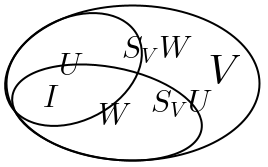
\includegraphics[width=80pt]{diagram3F-1}$\\\;\\\;}$\par\vspace{-42pt}\quad
%Now $0\neq x\in S_V I\Rightarrow\exists\,!\,\Par{u_v,i_u,w_v,i_w}\in S_V U\times S_U I\times S_V W\times S_W I,$\par\quad
%$x=u_v+i_u=w_v+i_w.$ Define $\varphi\in U^0,\beta\in W^0$ by $\varphi:u_v\mapsto 1,u\mapsto 0,$ and $\beta:i_u\mapsto 1,i\mapsto 0,$\par\quad
%for all $u\in\Pure V\XSlash\Span{u_v}$ and $i\in\Pure V\XSlash\Span{i_u}.$ \OR Define $\psi\in W^0,\gamma\in U^0,$ simlr.\par\quad
%Then $\varphi=\varphi+\beta=\psi+\gamma\in U^0+W^0.$\PfEnd
\AComm Not true if $U$ or $W$ is merely a subset. Promote $U\cap W$ as $I,$ \,$U$ as $X,$ \,and $W$ as $Y.$\par
%Now we show $X\cap Y=I.$ So that $\BigPar{U\cap W}{^0}=I^0=\BigPar{X\cap Y}{^0}=X^0+Y^0=U^0+W^0.$\parCom
\AExa Let $U=\Bra{\Par{x,x+1}\in\Rbb^2},W=\Rbb^2.$ Then $U\cap W=I=U\neq\Rbb^2=X\cap Y.$
\SepLine

%\BulletPointX\ACoro (1) $\BigPar{U\cap W}{^0}=U^0+W^0\supseteq U^0\cap W^0=\BigPar{U+W}{^0}.$\vspace{2pt}\parCor{\IndentB}
%(2) ${\envFontLarge\BigPar{{\envFontDefault\bigcap_{\alpha_i\in\Gamma}V_{\!\alpha_i}}}}{^0}=\sum_{\alpha_i\in\Gamma}\BigPar{V^0_{\!\alpha_i}},\;\;{\envFontLarge\BigPar{{\envFontDefault\sum_{\alpha_i\in\Gamma}V_{\!\alpha_i}}}}{^0}=\bigcap_{\alpha_i\in\Gamma}\BigPar{V^0_{\!\alpha_i}}.$
%\SepLine
\pagebreak

\ProblemB{
	\TipsN{1}\,\,\,\TextB{Prove $V=U\oplus W\Longleftrightarrow V\apostrophe=U^0\oplus W^0.$}
}$U\cap W=\zeroSubs\Longleftrightarrow \BigPar{U\cap W}{^0}=\zeroSubs{_V^0}=V\apostrophe=U^0+W^0.$\parSol{\vspace{1pt}}
$V=U+W\Longleftrightarrow\BigPar{U+W}{^0}=V_V^0=\zeroSubs=U^0\cap W^0.$\PfEnd
\SepLine

\ProblemB{
	\TextB{Supp $V=U\oplus W.$ Prove $U^0=\Bra{\varphi\in V\apostrophe:\varphi=\varphi\circ\iota},$ \FontNorm where $\iota\in\Lm{V,W}:u_v+w_v\rightarrow w_v$.}
%	\NewNotation\;\;Denote $W^0$ by $U_V\upapostrophe,$ and $U^0$ by $W_V\upapostrophe.$\TextB{}
}$\varphi\in U^0\Longleftrightarrow U\subseteq\null\varphi\Longleftrightarrow\varphi=\varphi\circ\iota,$ by \Sbra{3.B \TIPSN{3}}.\PfEnd\vspace{3pt}
\ANote The nota $W_V\upapostrophe=\Bra{\varphi\in V\apostrophe:\varphi=\varphi\circ\iota}=U^0$ is not well-defined \Sbra{without a bss}.\parNot
Simply becs $W_V\upapostrophe$ have no info about the given $U.$ Here is an informal explanation:\parNot
Each liney map $T\in\Lm{V,W}$ that vanishes on a given nontrivial $U$ has its '$P$'\parNot
\Par{ though not uniq } suth '$U\oplus P=V$' with $T:P\mapsto\range T$ being surj.\parNot
Hence $\forall W\in\mathcal{S}_V U,\,U^0=W_{V}'.$ But given nontrivial '$P$', the corres '$U$' is not uniq.\parNot
Fix one $W_V\upapostrophe,$ then $U^0$ is not uniq, with each $U_k$ not equal to each other while each $U_k^0=W_V\upapostrophe.$\par\vspace{3pt}
\AExa Let $B_V=\Par{e_1,e_2}.$ Let $B_U=\Par{e_1},B_X=\Par{e_2-e_1},B_Y=\Par{e_2}.$\parExa
Then $\iota_X:ae_1+b\Par{e_2-e_1}\mapsto b\Par{e_2-e_1},\;\;\iota_Y:ae_1+be_2\mapsto be_2.$ Now $X_V\upapostrophe=Y_V\upapostrophe=U^0.$\parExa
(1) For $V=U\oplus X,$ let $B_{U_V'}=\Par{\varphi}$ with $\varphi:e_1\mapsto 1,\;e_2-e_1\mapsto 0\Rightarrow e_2\mapsto 1.$\parExa
(2) For $V=U\oplus Y,$ let $B_{U_V'}=\Par{\psi}$ with $\psi:e_1\mapsto 1,e_2\mapsto 0.$\parExa
Thus $X^0=U_V\upapostrophe$ while $Y^0=U_V\upapostrophe\Rightarrow X^0=Y^0\Rightarrow X=Y,$ ctradic.\parExa
To fix this, we must have a bss of $V\apostrophe$ as precond, which we'll see in the {\NOTEFOR} Exa (31).\par\vspace{3pt}
\ANote {\tgsl Supp $U$ is a subsp of $V.$ Then finding the corres subsp in $V\apostrophe$ firstly req another 'half' $W\in\mathcal{S}_V U,$}\vspace{-2pt}\parNot
{\tgsl while finding the corres subsp of $V$ for a subsp of $V\apostrophe$ must have the another 'half' asumed as precond.}
\SepLine

\ProblemN{\hypertarget{3F31}{31}}{
	\TextNL{Supp $V$ is finide and $B_{V\apostrophe}=\Par{\varphi_1,\dots,\varphi_n}.$ Show $\exists\,!\,B_V$ whose dual bss is the $B_{V\apostrophe}$.}
}For each $k\in\Bra{1,\dots,n},$ let $\Gamma_k=\Bra{1,\dots,n}\Backslash[\Big]\Bra{k}.$ Let each $U_k=\bigcap_{j\in\Gamma}\null\varphi_j.$\parSol{}
By Exe (4E 23), $V\apostrophe=\Span{\varphi_1,\dots,\varphi_n}=\BigPar{\null\varphi_1\cap\cdots\cap\null\varphi_n}{^0}\Rightarrow U_k\cap\varphi_k=\zeroSubs.$\parSol{}
Thus $\forall x_k\in U_k\nonzero,\;x_k\not\in\null\varphi_k$ while $x_k\in\null\varphi_j$ for all $j\in\Gamma.$\parSol{}
Fix one $x_k$ and let $v_k=\Sbra{\varphi_k\Par{x_k}}{^{-1}}x_k\Rightarrow\varphi_k\Par{v_k}=1,\,\varphi_j\Par{v_k}=0$ for all $j\neq k.$\parSol{}
Simply for each $v_k,$ \,$\varphi_j\Par{v_k}=\delta_{j,k}$ for all $j\Longleftrightarrow$ for each $\varphi_j,$ $\varphi_j\Par{v_k}=\delta_{j,k}$ for all $k.$\parSol{}
又 $a_1v_1+\dots+a_nv_n=0\Rightarrow$ each $\varphi_k\Par{0}=a_k.$\vspace{2pt}\parSol{}
Now we prove the uniqnes part. Supp the dual bss of $B_V'=\Par{u_1,\dots,u_n}$ is the $B_{V\apostrophe}.$\parSol{}
For each $k,$ we have $\varphi_j\Par{v_k}=\varphi_j\Par{u_k}$ for all $k\Rightarrow v_k-u_k\in\bigcap\null\varphi_j=\zeroSubs.$\PfEnd
\SepLine

\BulletPointX\NoteForSmall{Exe (31)}\;\;Supp $V$ is finide, and $\Omega$ is a subsp of $V\apostrophe$ with $B_{\Omega}=\Par{\varphi_1,\dots,\varphi_m}.$\TextB{}
The '$W$' is not clear when we are to find suth $W_V\apostrophe=\Omega,$ becs the another 'half' is undefined.\TextB{}
Extend to $B_{V\apostrophe}=\Par{\varphi_1,\dots,\varphi_n}.$ By Exe (31), $\exists\,!\,$corres $B_V=\Par{v_1,\dots,v_n}.$\TextB{}
Let $B_U=\Par{v_{m+1},\dots,v_n},B_W=\Par{v_1,\dots,v_m}.$ \,Thus we found the $W$ suth $\Omega=W_V\upapostrophe,$\TextB{}
which is well-defined with $B_V$ as precond.
\SepLine
}
%\def\OrbikenII
{
\BulletPointX\TipsN{2}\,\,\,Supp $\varphi_1,\dots,\varphi_m\in V\apostrophe.$ Let $\null_I=\Par{\null\varphi_1}\cap\dots\cap\Par{\null\varphi_m}.$\TextB{}
\IndentTipsN{2}Supp $\Omega$ is a subsp of $V\apostrophe.$ Let $\null_C=\Bra{v\in V:\varphi\Par{v}=0,\forall\varphi\in\Omega}.$\TextB{\vspace{2pt}}
(1) If $\Omega$ is infinide. Then by def, $\bigcap_{\varphi\,\in\,\Omega}\null\varphi=\null_C.$\TextB{\vspace{1pt}}
(2) If $\Omega=\Span{\varphi_1,\dots,\varphi_m}.$ Then $v\in\null_I\Longleftrightarrow$ each $\varphi_k\Par{v}=0$\TextB{}
\Blind{(2) If $\Omega=\Span{\varphi_1,\dots,\varphi_m}.$ Then $v\in\null_I$}${}\Longleftrightarrow\forall\varphi=\sum_{i=1}^na_i\varphi_i\in\Omega,\varphi\Par{v}=0\Longleftrightarrow v\in\null_C.$
\SepLine\pagebreak

\ProblemBnoor{4E 23}{
	\TextB{Supp $V$ is finide, $\Omega=\Span{\varphi_1,\dots,\varphi_m}\subseteq V\apostrophe.$ Prove $\Omega=\BigPar{\null\varphi_1\cap\cdots\cap\null\varphi_m}{^0}.$}
}Becs each $\Span{\varphi_k}\subseteq\Par{\null\varphi_k}{^0}.$ By {\NOTEFOR} Exe (4E 23) and Exe (23), Immed.\PfEnd\parSol{\vspace{4pt}}
\Or Reduce to $B_{\Omega}=\Par{\beta_1,\dots,\beta_p}.$ We show $\Omega=\Par{\null\beta_1\cap\cdots\cap\null\beta_p}{^0}.$ Then by (L1), done.\parSol{}
Let $B_{V\apostrophe}=\Par{\beta_1,\dots,\beta_p,\gamma_1,\dots,\gamma_q}.$ By Exe (31), let $B_V=\Par{v_1,\dots,v_p,u_1,\dots,u_q}.$\parSol{}
Define each $\Gamma_k=\Bra{1,\dots,p}\Backslash[\Big]\Bra{k}.$ Then $\null\beta_k=\Spn\Bra{v_j}{_{j\in\Gamma_k}}\oplus\Span{u_1,\dots,u_q}.$\parSol{}
Now $\null\beta_1\cap\cdots\cap\null\beta_p=\Span{u_1,\dots,u_q}.$ Simlr to (4E 2.C.16).\parSol{}
Supp $\varphi=\sum_{i=1}^pa_i\beta_i+\sum_{j=1}^qb_j\gamma_j\in\Span{u_1,\dots,u_q}{^0}.$ Then each $\varphi\Par{u_k}=0=b_k$\parSol{}
Thus $\Span{u_1,\dots,u_q}{^0}\subseteq\Span{\beta_1,\dots,\beta_p}=\Omega.$\PfEnd
\SepLine

\ProblemN{L1}{
	\TextLN{Supp each $\varphi_i,\beta_j\in\Lm{V,W}.$ Supp $\Span{\varphi_1,\dots,\varphi_m}=\Span{\beta_1,\dots,\beta_n}.$}
	\TextLN{Prove $\null\varphi_1\cap\dots\cap\null\varphi_m=\null\beta_1\cap\dots\cap\null\beta_n.$\vspace{1pt}}
}Denote $\null\psi_a\cap\cdots\cap\null\psi_b$ by $\bigcap_a^b\null\psi_I.$ Becs each $\beta_k\in\Span{\varphi_1,\dots,\varphi_m}.$\parSol{}
$\forall v\in\bigcap_1^m\null\varphi_I,\beta_k\Par{v}=0.$ Thus $\bigcap_1^m\null\varphi_I\subseteq\bigcap_1^n\null\beta_I.$ \;Rev the roles and done.\PfEnd\vspace{2pt}
\ANote Supp $\varphi_j=c_1\varphi_1+\dots+c_{j-1}\varphi_{j-1}.$\parNot{\vspace{2pt}}
Let $N_j\oplus\bigcap_1^{j-1}\null\varphi_I=\null\varphi_j.$ Now $\bigcap_1^j\null\varphi_I=\bigcap_1^{j-1}\null\varphi_I\cap\BigPar{\null\varphi_j}=\bigcap_1^{j-1}\null\varphi_I.$\parNot{\vspace{2pt}}
Thus $\bigcap_1^m\null\varphi_I=\Sbra{\bigcap_1^{j-1}\null\varphi_I}\cap\Sbra{\bigcap_{j+1}^m\null\varphi_I}.$ \;Hence $\bigcap_1^n\null\beta_I=\bigcap_{1}^m\null\varphi_I.$
\SepLine

%For each $\varphi_k=0,$ $\Span{\varphi_k}=\zeroSubs=\BigPar{\null\varphi_k}{^0}.$\par\quad\Ha
%For each $\varphi_k\neq 0.$ Using (3.B.29) and {\TIPSN{1}}. Let $\varphi\Par{v_k}\neq 0\Rightarrow\null\varphi_k\oplus\Span{v_k}=V.$\par\quad\Ha
%Then $\BigPar{\null\varphi_k}{^0}=\BigPar{\Span{v_k}}{_V\upapostrophe}=\Bra{\varphi\in V\apostrophe:\varphi=\varphi\circ\iota}=\Span{\varphi_k},$ where $\iota:cv_k+u_0\rightarrow cv_k.$\par\quad\Ha
%Thus $\Omega=\Span{\varphi_1}+\dots+\Span{\varphi_m}=\BigPar{\null\varphi_1}{^0}+\dots+\BigPar{\null\varphi_m}{^0}$\par\quad\Ha
%\Blind{Thus $\Omega=\Span{\varphi_1}+\dots+\Span{\varphi_m}$}${}=\BigPar{\Par{\null \varphi_1}\cap\dots\cap\Par{\null \varphi_m}}{^0}=\BigPar{\null_I}{^0}.$\PfEnd\vspace{4pt}\quad\Ha

\ProblemN{\hypertarget{3F26}{26}}{
	\TextB{Supp $V$ is finide, $\Omega$ is a subsp of $V\apostrophe.$ Prove $\Omega=\Bra{v\in V:\varphi\Par{v}=0\text{ for every }\varphi\in\Omega}{^0}.$}
}Let $B_{\Omega}=\Par{\varphi_1,\dots,\varphi_m}.$ By {\TIPSN{2}} and Exe (4E 23).\PfEnd\vspace{1pt}
\AExa Denote $\Bra{v\in V:\varphi\Par{v}=0\text{ for every }\varphi\in\Omega}$ by $\Omega_{\perp}.$ Then immed, $\Omega\subseteq\Par{\Omega_{\perp}}{^0}.$\parExa
Let $V=\Bra{\Par{x_1,x_2,\cdots}\in\Fbb^{\infty}:x_k\neq 0\text{ for only finily many }k}.$ Then $V\apostrophe=\Par{\Fbb^{\infty}}\apostrophe.$\parExa
Let $\Omega=\Bra[\envFontA]{\varphi\in\Span{\varphi_{\alpha_1},\dots,\varphi_{\alpha_m}}:\exists\:m,\alpha_k\in\Nbp}\subsetneq V\apostrophe.$\parExa
Then $\Omega_{\perp}=\zeroSubs\Rightarrow\Par{\Omega_{\perp}}{^0}=V\apostrophe.$ Forming a counterexa for $\Omega\supseteq\Par{\Omega_{\perp}}{^0}.$\par\vspace{2pt}
\ACoro Supp $V$ is finide. For every subsp $\Omega$ of $V\apostrophe,\;\exists\,!\,$subsp $U$ of $V$ suth $\Omega=U^0.$\vspace{-2pt}\parCor
{\FontSmall\tgsl This form of $\Omega$ does not depend on a bss and thus is considered more general.}\vspace{-2pt}\par
\SepLine

%For nota convienence of understanding, let $\null_C=\Bra{v\in V:\varphi\Par{v}=0,\forall\varphi\in\Omega}.$\par\quad
%又 $\null_C=\Bra{v\in V:\varphi\Par{v}=0,\forall\varphi\in\BigPar{\null_C}{^0}}.$\par\quad
%$\forall\varphi\in\Omega,\null_C\subseteq\null\varphi\Rightarrow\varphi\in\BigPar{\null_C}{^0}.$ Hence $\Omega\subseteq\BigPar{\null_C}{^0}.$\par\quad
%Asum $\Omega\subsetneq\BigPar{\null_C}{^0}.$ Supp $\psi\in\BigPar{\null_C}{^0}\Backslash\Omega.$\par\quad
%Let $\null\psi\oplus\Span{w}=V.$ Then supp $\varphi\in\Omega\nonzero\subseteq\BigPar{\null_C}{^0}.$\par\quad
%Let $\null\varphi\oplus\Span{v}=V.$ Then let $\Theta\oplus\null_C=\null\psi,\;\Delta\oplus\null_C=\null\varphi.$\par\quad
%Thus $V=\Theta\oplus\null_C\oplus\Span{w}=\Delta\oplus\null_C\oplus\Span{v}.$ Now we show $\psi\in\Omega.$\par\quad
%\PfEnd\vspace{6pt}


%\ProblemN{24}{
%	\TextNL{Supp $V$ is finide and $U$ is a subsp of $V$.}
%	\TextNL{Prove, using the pattern of [3.104], that $\dim U+\dim U^0=\dim V$.}
%}Let $B_U=\Par{u_1,\dots,u_m},B_V=\Par{u_1,\dots,u_m,v_1,\dots,v_n},B_{V\apostrophe}=\Par{\psi_1,\dots,\psi_m,\varphi_1,\dots,\dots\varphi_n}.$\parSol{}
%Supp $\psi=\sum_{i=1}^ma_i\psi_i+\sum_{j=1}^nb_j\varphi_j\in U^0\Rightarrow$ each $\psi\Par{u_k}=a_k=0.$ Thus $U^0\subseteq\Span{\varphi_1,\dots,\varphi_n}.$\PfEnd
%\SepLine

\BulletPointX\TipsN{3}\,\,\,Let $B_{U^0}=\Par{\varphi_1,\dots,\varphi_m},B_{V\apostrophe}=\Par{\varphi_1,\dots,\varphi_n}\Rightarrow B_V=\Par{v_1,\dots,v_n}.$\TextB{}
We show $B_U=\Par{v_{m+1},\dots,v_n}.$ Let $B_{W^0}=\Par{\varphi_{m+1},\dots,\varphi_n}.$\TextB{}
And let corres (I) $B_U=\Par{v_{m+1},\dots,v_n},$ \; (II) $B_W=\Par{v_1,\dots,v_m}.$\TextB{}
%$V\apostrophe=\Span{\varphi_1,\dots,\varphi_m}\oplus\Span{\varphi_{m+1},\dots,\varphi_n}=\Span{v_{m+1},\dots,v_n}{^0}\oplus\Span{v_1,\dots,v_m}{^0}.$\TextB{}
%$\Span{\varphi_1,\dots,\varphi_m}=\Span{v_{m+1},\dots,v_n}{^0}=U{^0};\;\Span{\varphi_{m+1},\dots,\varphi_n}=\Span{v_1,\dots,v_m}{^0}=W^0.$\TextB{}
%Supp for each $\varphi_k,$ let $\mathcal{K}_k$ be suth $V=\mathcal{K}_k\oplus\null\varphi_k.$ By (3.B.29), this $\mathcal{K}_k$ can be $\Span{v_k}.$\TextB{}\HI
%Then ${\mathcal{K}_1}+\dots+{\mathcal{K}_k}=\Span{v_1,\dots,v_k}.$\TextB{}\HI
(I) \NOTICE that each $\null\varphi_k=\Span{v_1,\dots,v_{k-1},v_{k+1},\dots,v_n}=U_k;\;\dim U_k=\dim V-1.$\TextB{}
\HI By (4E 2.C.16), $U=\Par{\null\varphi_1}\cap\cdots\cap\Par{\null\varphi_m}=\bigcap_{k=1}^m U_k=\Span{v_{m+1},\dots,v_n}.$\TextB{}
\HI Hence $\Span{v_{m+1},\dots,v_n}{^0}=U^0=\Omega=\Span{\varphi_1,\dots,\varphi_m}.$\vspace{2pt}\TextB{}
\EndI (II) \NOTICE that $V\apostrophe=\Omega\oplus\Span{\varphi_{m+1},\dots,\varphi_n}=U^0\oplus\Span{v_1,\dots,v_m}{^0}.$\TextB{}
\HII And that $\Span{\varphi_{m+1},\dots,\varphi_n}\subseteq\Span{v_1,\dots,v_m}{^0}.$\TextB{}
\HII By \Sbra{1.C \TIPSN{2}} \OR (2.C.1), $\Span{\varphi_{m+1},\dots,\varphi_n}=\Span{v_1,\dots,v_m}{^0}.$\TextB{}
\HII \Or Simlr to (II), let $\Omega=\Span{\varphi_{m+1},\dots,\varphi_n},$ immed.\PfEnd
\SepLine

%\ProblemB{
%	\TextB{Supp $T\in\Lm{V,W},\varphi_k\in V\apostrophe,\psi_k\in W\apostrophe.$}
%	\ProblemN[]{}{}
%	\ProblemN[]{\hypertarget{3F28}{28}}{
%		\TextNL{Prove $\null T\apostrophe=\Span{\psi_1,\dots,\psi_m}\Longleftrightarrow\range T=\Par{\null\psi_1}\cap\cdots\cap\Par{\null\psi_m}.$}}
%	\ProblemN[]{\hypertarget{3F29}{29}}{
%		\TextNL{Prove $\range T\apostrophe=\Span{\varphi_1,\dots,\varphi_m}\Longleftrightarrow\null T=\Par{\null\varphi_1}\cap\cdots\cap\Par{\null\varphi_m}.$}}
%	\TextB{\vspace{-4pt}}
%}Using [3.107], [3.109], Exe (23) and the {\COROLLARY} in Exe (20, 21).\par\quad
%(28) $\Par{\range T}{^0}=\null T\apostrophe=\Span{\psi_1,\dots,\psi_m}=\BigPar{\Par{\null\psi_1}\cap\cdots\cap\Par{\null\psi_m}}{^0}.$\par\quad
%(29) $\Par{\null T}{^0}=\range T\apostrophe=\Span{\varphi_1,\dots,\varphi_m}=\BigPar{\Par{\null\varphi_1}\cap\cdots\cap\Par{\null\varphi_m}}{^0}.$\PfEnd\vspace{6pt}
%\Corollary\,\,\,Using the \COMMENT in Exe (26).\par\quad
%$\null T=\Span{v_1,\dots,v_m}\Longleftrightarrow\null T=\Par{\null\varphi_{m+1}}\cap\cdots\cap\Par{\null\varphi_n}\Longleftrightarrow\range T\apostrophe=\Span{\varphi_{m+1},\dots,\varphi_n}.$\par\quad
%——Where $B_V=\Par{v_1,\dots,v_m,\dots,v_n}\Longleftrightarrow B_{V\apostrophe}=\Par{\varphi_1,\dots,\varphi_m,\dots,\varphi_n}.$\vspace{3pt}\par\quad
%$\range T=\Span{w_1,\dots,w_m}\Longleftrightarrow\range T=\Par{\null\psi_{m+1}}\cap\cdots\cap\Par{\null\psi_n}\Longleftrightarrow\null T\apostrophe=\Span{\psi_{m+1},\dots,\psi_n}.$\par\quad
%——Where $B_W=\Par{w_1,\dots,w_m,\dots,w_n}\Longleftrightarrow B_{W\apostrophe}=\Par{\psi_1,\dots,\psi_m,\dots,\psi_n}.$\par
%\SepLine
}
\pagebreak
%\def\OrbikenIII
{
\ProblemN{\hypertarget{3F9}{9}}{
	\TextN{Let $B_V=\Par{v_1,\dots,v_n},\,B_{V\apostrophe}=\Par{\varphi_1,\cdots,\varphi_n}$. Then $\forall\psi\in V\apostrophe,\psi=\psi\Par{v_1}\varphi_1+\dots+\psi\Par{v_n}\varphi_n.$}
	\ACoro {\tgsl For other $B_V'=\Par{u_1,\dots,u_n},B_{V\apostrophe}'=\Par{\rho_1,\dots,\rho_n},\forall\psi\in V\apostrophe,\psi=\psi\Par{u_1}\rho_1+\dots+\psi\Par{u_n}\rho_n.$}\TextB{}
}\par\quad
$\psi\Par{v}=\psi\XPar{\sum_{i=1}^n a_i v_i}=\sum_{i=1}^n a_i\psi\Par{v_i}=\sum_{i=1}^n\psi\Par{v_{i}}\varphi_i\Par{v}=\Sbra{\psi\Par{v_1}\varphi_1+\dots+\psi\Par{v_n}\varphi_n}\Par{v}.$\vspace{2pt}\par\quad
\Or $\Sbra{\psi\Par{v_1}\varphi_1+\dots+\psi\Par{v_n}\varphi_n}\XPar{\sum_{i=1}^n a_i v_i}=\psi\Par{v_1}\varphi_1\XPar{\sum_{i=1}^n a_i v_i}+\dots+\psi\Par{v_n}\varphi_n\XPar{\sum_{i=1}^n a_i v_i}.$\PfEnd
\SepLine

\ProblemN[]{\hypertarget{3F13}{13}}{
	\TextNL{Define $T:\Rbb^3\!\rightarrow\!\Rbb^2$ by $T\Par{x,y,z}=\Par{4x+5y+6z,7x+8y+9z}$.\vspace{3pt}}
	\TextNL{Let $\Par{\varphi_1,\varphi_2},\Par{\psi_1,\psi_2,\psi_3}$ denote the dual bss of std bss of $\Rbb^2$ and $\Rbb^3$.\vspace{4pt}}
	(a) \TextNL{Describe the liney functionals $T\apostrophe\Par{\varphi_1},T\apostrophe\Par{\varphi_2}\in\Lm{\Rbb^3,\Rbb}$\vspace{3pt}}
	\Ha\TextNL{{\FontNorm\tgnr For any $\Par{x,y,z}\in\Rbb^3$, $\BigPar{T\apostrophe\Par{\varphi_1}}\Par{x,y,z}=4x+5y+6z, \BigPar{T\apostrophe\Par{\varphi_2}}\Par{x,y,z}=7x+8y+9z$.}\vspace{8pt}}
	(b) \TextNL{Write $T\apostrophe\Par{\varphi_1}$ and $T\apostrophe\Par{\varphi_2}$ as liney combinations of $\psi_1,\psi_2,\psi_3$.\vspace{2pt}}
	\Hb\TextNL{{\FontNorm\tgnr$T\apostrophe\Par{\varphi_1}=4\psi_1+5\psi_2+6\psi_3,\,\,T\apostrophe\Par{\varphi_2}=7\psi_1+8\psi_2+9\psi_3.$}\vspace{8pt}}
	(c) \TextNL{What is $\null T\apostrophe$? What is $\range T\apostrophe$?}
}\TextNL{\vspace{4pt}}
\Hc $T\Par{x,y,z}=0\Longleftrightarrow\MathLeftBrace{l}{4x+5y+6z=0\\7x+8y+9z=0}\Longleftrightarrow \MathLeftBrace{l}{x+y+z=0\\y=2z=0}\Longleftrightarrow\Par{x,y,z}\in\Span{e_1-2e_2+e_3}.$\vspace{3pt}\TextNL{}
\Hc Where $\Par{e_1,e_2,e_3}$ is std bss of $\Rbb^3.$\vspace{1.5pt}\TextNL{}
\Hc Let $\Par{e_1-2e_2+e_3,-2e_2,e_3}$ be a bss, with corres dual bss $\Par{\varepsilon_1,\varepsilon_2,\varepsilon_3}$.\vspace{1.5pt}\TextNL{}
\Hc Thus $\Span{e_1-2e_2+e_3}=\null T\Rightarrow \Span{e_1-2e_2+e_3}{^0}=\Span{\varepsilon_2,\varepsilon_3}=\range T\apostrophe.$\vspace{1.5pt}\TextNL{}
\Hc Note that $\varepsilon_k=\varepsilon_k\Par{e_1}\psi_1+\varepsilon_k\Par{e_2}\psi_2+\varepsilon_k\Par{e_3}\psi_3.$\vspace{1.5pt}\TextNL{}
\Hc And $\MathLeftMid{l}{\varepsilon_2\Par{e_2}=-\frac{\;1\;}{2},\varepsilon_2\Par{e_1}=\varepsilon_2\Par{e_1-2e_2+e_3}+\varepsilon_2\Par{2e_2}-\varepsilon_2\Par{e_3}=1,\\[1.5pt]\varepsilon_3\Par{e_2}=0,\varepsilon_3\Par{e_3}=\varepsilon_3\Par{e_1-2e_2+e_3}+\varepsilon_3\Par{2e_2}-\varepsilon_3\Par{e_3}=-1.}$\vspace{1.5pt}\TextNL{}
\Hc Hence $\varepsilon_2=\psi_1-\frac{\;1\;}{2}\psi_2,\;\varepsilon_3=-\psi_1+\psi_3.$ Now $\range T\apostrophe=\Span{\psi_1-\frac{\;1\;}{2}\psi_2,-\psi_1+\psi_3}.$\vspace{4.5pt}\TextNL{}
\Hc\Or $\range T\apostrophe=\Span{T\apostrophe\Par{\varphi_1},T\apostrophe\Par{\varphi_2}}=\Span{4\psi_1+5\psi_2+6\psi_3,7\psi_1+8\psi_2+9\psi_3}.$\vspace{7.5pt}\TextNL{}
\Hc Supp $T\apostrophe\Par{x\varphi_1+y\varphi_2}=\Par{4x+7y}\varphi_1+\Par{5x+8y}\varphi_2+\Par{6x+9y}\varphi_3=0.$\TextNL{}
\Hc Then $x+y=4x+7y=x=y=0.$ Hence $\null T\apostrophe=\zeroSubs.$\vspace{4.5pt}\TextNL{}
\Hc\Or $\null T=\Span{e_1-2e_2+e_3}\Rightarrow V=\Span{-2e_2,e_3}\oplus\null T.$\vspace{1.5pt}\TextNL{}
\Hc$\Rightarrow \range T=\Bra{Tx:x\in\Span{-2e_2,e_3}}=\Span{T\Par{-2e_2},T\Par{e_3}}$\vspace{1.5pt}\TextNL{}
\Hc$=\Span{-10f_1-16f_2,6f_1+9f_2}=\Span{f_1,f_2}=\Rbb^2.$ Now $\null T\apostrophe=\Par{\range T}{^0}=\zeroSubs.$\PfEnd\vspace{-2pt}
\SepLine

%\ProblemN[]{\hypertarget{3F14}{14}}{
%	\TextNL{Define $T:\PoRi\rightarrow\PoRi$ by $\Par{Tp}\Par{x}=x^2 p\Par{x}+p\apostrophe\apostrophe\Par{x}$ for each $x\in\Rbb.$\vspace{4pt}}
%	(a) \TextNL{Supp $\varphi\in\PoRi\apostrophe$ is defined by $\varphi\Par{p}=p\apostrophe\Par{4}$. Describe $T\apostrophe\Par{\varphi}\in\PoRi\apostrophe$.\vspace{4pt}}
%	\Ha\TextNL{\FontNorm$\BigPar{T\apostrophe\Par{\varphi}}\Par{p}=\Sbra{x^2p\Par{x}+p\apostrophe\apostrophe\Par{x}}\apostrophe\Par{4}=\Sbra{2xp\Par{x}+x^2p\apostrophe\Par{x}+p\apostrophe\apostrophe\apostrophe\Par{x}}\Par{4}=8p\Par{4}+16p\apostrophe\Par{4}+p\apostrophe\apostrophe\apostrophe\Par{4}$.\vspace{8pt}}
%	(b) \TextNL{Supp $\varphi\in\PoRi\apostrophe$ is defined by $\varphi\Par{p}=\int_0^1 p\Par{x}\d x$. Evaluate $\BigPar{T\apostrophe\Par{\varphi}}\Par{x^3}$.\vspace{4pt}}
%	\Hb\TextNL{\FontNorm $\BigPar{T\apostrophe\Par{\varphi}}\Par{x^3}=\int_0^1\Par{x^5+6x}\d x=\int_0^1\XPar{\frac{1}{6}x^6+3x^2}\apostrophe\d x=\frac{19}{6}.$\PfEnd}
%}\SepLine
}

%\def\OrbikenIV
{
%\Or Let $B_U=\Par{u_1,\dots,u_m},\,B_V=\Par{u_1,\dots,u_m,\dots,u_n},\,B_{V\apostrophe}=\Par{\varphi_1,\dots,\varphi_m,\dots,\varphi_n}$.\par\quad
%We show ${U^0}=\Span{\varphi_{m+1},\dots,\varphi_n}.$ So that $\dim U^0=n-m=\dim V-\dim U.$\par\quad
%$\forall\varphi\in U^0,\exists\,a_i\in\Fbb,\varphi=\sum_{i=1}^m a_i\varphi_i+\sum_{i=m+1}^n a_i\varphi_i$ 又 $\forall i\in\Bra{1,\dots,m},\varphi\Par{u_i}=0\Rightarrow a_i=0.$\par\quad
%Then $\varphi\in\Span{\varphi_{m+1},\dots,\varphi_n}$. Thus $\Span{\varphi_{m+1},\dots,\varphi_n}\supseteq U^0.$ 又 Each $\varphi_i\in U^0.$

\ProblemN{\hypertarget{3F37}{37}}{
	\TextNL{Supp $U$ is a subsp of $V$ and $\pi$ is the quot map. Thus $\pi\apostrophe\in\Lm[\BigPar]{\Par{V\XSlash U}\apostrophe,V\apostrophe}$.\vspace{2pt}}
	(a) \TextNL{Show $\pi\apostrophe$ is inje\hspace{1pt}$:${\tgnr\FontNorm\;\;Becs $\pi$ is surj. Use [3.108].}\vspace{2pt}}
	(b) \TextNL{Show $\range \pi\apostrophe=U^0$\hspace{1pt}$:${\tgnr\FontNorm\;\;By {\tgnr[3.109](b)}, $\range\pi\apostrophe=\BigPar{\null\pi}{^0}=U^0.$}\vspace{2pt}}
	(c) \TextNL{Conclude that $\pi\apostrophe$ is iso from $\Par{V\XSlash U}\apostrophe$ onto $U^0$\hspace{1pt}$:${\tgnr\FontNorm\;\;Immed.}}
}\Or Using (3.E.18), also see (3.E.20).\par\quad
(a) $\pi\apostrophe\Par{\varphi}=0\Longleftrightarrow\forall v\in V\,\BigPar{\,\forall v+U\in V\,},\varphi\BigPar{\pi\Par{v}}=\varphi\Par{v+U}=0\Longleftrightarrow \varphi=0.$\par\quad
(b) $\psi\in\range\pi\apostrophe\Longleftrightarrow\exists\,\varphi\in \Par{V\XSlash U}\apostrophe,\psi=\varphi\,\circ\,\pi\Longleftrightarrow\null\psi\supseteq U\Longleftrightarrow \psi\in U^0$. Hence $\range\pi\apostrophe=U^0$.\PfEnd
\SepLine

\pagebreak

\ProblemB{
	\TextB{Supp $U$ is a subsp of $V.$ Prove $\Par{V\XSlash U}\apostrophe$ is iso to $U^0.$ \hfill\Sbra[3pt]{{\large\tgsc Another proof of \tgbfx[3.106]}}}
}\par\quad
Define $\xi:U^0\rightarrow\Par{V\XSlash U}\apostrophe$ by $\xi\Par{\varphi}=\tilde{\varphi},$ where $\tilde{\varphi}\in\Par{V\XSlash U}\apostrophe$ is defined by $\tilde{\varphi}\Par{v+U}=\varphi\Par{v}.$\vspace{4pt}\par\quad
We show $\xi$ is inje and surj.\par\quad
Inje: $\xi\Par{\varphi}=0=\tilde{\varphi}\Rightarrow\forall v\in V\,\BigPar{\,\forall v+U\in V\XSlash U\,},\tilde{\varphi}\Par{v+U}=\varphi\Par{v}=0\Rightarrow\varphi=0.$\par\quad
Surj: $\varPhi\in\Par{V\XSlash U}\apostrophe\Rightarrow\forall u\in U,\varPhi\Par{u+U}=\varPhi\Par{0+U}=0\Rightarrow U\subseteq\null\Par{\varPhi\circ\pi}\Rightarrow\xi\Par{\varPhi\circ\pi}=\varPhi.$\PfEnd\vspace{4pt}\quad
\Or Define $\nu:\Par{V\XSlash U}\apostrophe\rightarrow U^0$ by $\nu\Par{\varPhi}=\varPhi\circ\pi.$ Now $\nu\circ\xi=I_{U^0},\;\xi\circ\nu=I_{\SmallPar[1pt]{V\XSlash U}\apostrophe}\Rightarrow\xi=\nu^{-1}.$\PfEnd\vspace{-2pt}
\SepLine

}

%\def\OrbikenV
{
}

%\def\OrbikenVI
{
\ProblemB{
	\TextB{Supp $V=U\oplus W$. Define $\iota:V\rightarrow U$ by $\iota\Par{u+w}=u.$ Thus $\iota\apostrophe\in\Lm{U\apostrophe,V\apostrophe}.$\vspace{2pt}}
	(a) \TextB{Show $\null \iota\apostrophe=U_U^0=\zeroSubs$\hspace{1pt}$:${\tgnr\FontNorm\;\;$\null\iota\apostrophe=\Par{\range\iota}{^0_U}=U_U^0=\zeroSubs.$}\vspace{2pt}}
	(b) \TextB{Prove $\range\iota\apostrophe=W_V^0$\hspace{1pt}$:${\tgnr\FontNorm\;\;$\range\iota\apostrophe=\BigPar{\null\iota}{^0_V}=W_V^0.$}\vspace{2pt}}
	(c) \TextB{Prove $\tilde{\iota\apostrophe}$ is iso from $U\apostrophe\XSlash{\envFontDefault\zeroSubs}$ onto $W^0$\hspace{1pt}$:${\tgnr\FontNorm\;\;By (a), (b) and [3.91](d).}}
}\par\quad
(a) $\iota\apostrophe\Par{\psi}=\psi\circ\iota=0\Longleftrightarrow U\subseteq\null\psi.$\par\quad
(b) Note that $W=\null\Par{\iota}\subseteq\null\Par{\psi\circ\iota}.$ Then $\psi\circ\iota\in W^0\Rightarrow\range\iota\apostrophe\in W^0.$\par\quad\Hb
Supp $\varphi\in W^0.$ Becs $\null\iota=W\subseteq\null\varphi.$ By \Sbra{3.B \TIPSN{3}}, $\varphi=\varphi\circ\iota=\iota\apostrophe\Par{\varphi}.$\PfEnd
\SepLine

\ProblemN{\hypertarget{3F36}{36}}{
	\TextNL{Supp $U$ is a subsp of $V$. Define $i:U\rightarrow V$  by $i\Par{u}=u$. Thus $i\apostrophe\in\Lm{V\apostrophe,U\apostrophe}.$\vspace{2pt}}
	(a) \TextNL{Show $\null i\apostrophe=U^0$\hspace{1pt}$:${\tgnr\FontNorm\;\;$\null i\apostrophe=\Par{\range i}{^0}=U^0\Leftarrow\range i=U$.}\vspace{2pt}}
	(b) \TextNL{Prove $\range i\apostrophe=U\apostrophe$\hspace{1pt}$:${\tgnr\FontNorm\;\;$\range i\apostrophe=\Par{\null i}{_U^0}={\zeroSubs}{_U^0}=U\apostrophe$.}\vspace{2pt}}
	(c) \TextNL{Prove $\tilde{i\apostrophe}$ is iso from $V\apostrophe\XSlash U^0$ onto $U\apostrophe$\hspace{1pt}$:${\tgnr\FontNorm\;\;By (a), (b) and [3.91](d).}\vspace{2pt}}
}\par\quad
(a) $\forall\varphi\in V\apostrophe,i\apostrophe\Par{\varphi}=\varphi\circ i=\varphi\mmid_U.$ Thus $i\apostrophe\Par{\varphi}=0\Longleftrightarrow\forall u\in U,\varphi\Par{u}=0\Longleftrightarrow\varphi\in U^0.$\par\quad
(b) Supp $\psi\in U\apostrophe.$ By (3.A.11), $\exists\,\varphi\in V\apostrophe,\varphi\mmid_U=\psi.$ Then $i\apostrophe\Par{\varphi}=\psi.$\PfEnd
\SepLine

\ProblemB{
	\TextB{Supp $T\in\Lm{V,W}.$ Prove $\range T\apostrophe=\BigPar{\null T}{^0}.$\hfill\Sbra[3pt]{{\tgsc\large Another proof of \tgnr\tgbfx[3.109](b)}}}
}\par\quad
Supp $\varPhi\in\BigPar{\null T}{^0}.$ Becs by (3.B.12), $T\mmid_U:U\rightarrow\range T$ is iso; $V=U\oplus\null T.$\par\quad
And $\forall v\in V,\exists\,!\,u_v\in U,w_v\in\null T,v=u_v+w_v.$ Define $\iota\in\Lm{V,U}$ by $\iota\Par{v}=u_v.$\vspace{4pt}\par\quad
Let $\psi=\varPhi\circ\BigPar{T^{-1}\mmid_{\range T}}.$ Then $T\apostrophe\Par{\psi}=\psi\circ T=\varPhi\circ\BigPar{T^{-1}\mmid_{\range T}\circ T\mmid_V}.$\vspace{2pt}\par\quad
Where $T^{-1}\mmid_{\range T}:\range T\rightarrow U;\;\;T:V\rightarrow\range T.$ Note that $T^{-1}\mmid_{\range T}\circ T\mmid_V=\iota.$\vspace{2pt}\par\quad
By \Sbra{3.B \TIPSN{3}}, $\varPhi=\varPhi\circ \iota.$ Thus $T\apostrophe\Par{\psi}=\psi\circ T=\varPhi\circ{\iota}=\varPhi.$\PfEnd
\SepLine
}

%\def\OrbikenVII
{
\ProblemB[]{
	\hypertarget{3F4e17}{}\TextB{Supp $T\in\Lm{V,W}.$ {\large Using [3.108], [3.110].}\vspace{4pt}}
	\TextB{Now $T$ is inv $\Longleftrightarrow{}${$\envFontDefault\large\MathLeftrightMid{c}{
		\null T=\zeroSubs\Longleftrightarrow\BigPar{\null T}{^0}=V\apostrophe=\range T\apostrophe\\
		\range T=W\Longleftrightarrow\Par{\range T}{^0}=\zeroSubs=\null T\apostrophe
		}$}${}\Longleftrightarrow T\apostrophe$ is inv.\vspace{4pt}}
}\SepLine
\pagebreak
\ProblemN{\hypertarget{3F15}{15}}{
	\TextNL{Supp $T\in\Lm{V,W}$. Prove $T\apostrophe=0\Longleftrightarrow T=0.$}
}\par\quad
Supp $T=0.$ Then $\forall\varphi\in W\apostrophe,T\apostrophe\Par{\varphi}=\varphi\circ T=0.$ Hence $T\apostrophe=0.$\par\quad
Supp $T\apostrophe=0.$ Then $\null T\apostrophe=W\apostrophe=\Par{\range T}{^0},$  by [3.107](a).\par\quad
\!\Sbra[3pt]{{\tgsl$W$ can be infinide}} \;By Exe (25),\par\qquad
$\range T=\Bra{w\in W:\varphi\Par{w}=0,\forall\varphi\in\Par{\range T}{^0}}=\Bra{w\in W:\varphi\Par{w}=0,\forall\varphi\in W\apostrophe}.$\par\quad
Now we prove if $\forall\varphi\in W\apostrophe,\varphi\Par{w}=0,$ then $w=0.$ So that $\range T=\zeroSubs$ and done.\par\quad
Asum $w\neq 0.$ Then let $U$ be suth $W=U\oplus\Span{w}.$\par\quad
Define $\psi\in W\apostrophe$ by $\psi\Par{u+\lambda w}=\lambda.$ So that $\psi\Par{w}=1\neq 0.$\PfEnd\vspace{6pt}\quad
\Or \Sbra[3pt]{{\tgsl Only if $W$ is finide}} \;By [3.106], $\dim \range T=\dim W-\Dim\Par{\range T}{^0}=0.$\PfEnd
\SepLine

\ProblemN[]{\hypertarget{3F12}{12}}{
	\TextNL{{\large\tgnr\NOTICE that $I_{V\apostrophe}:V\apostrophe\rightarrow V\apostrophe.$} Now $\forall\varphi\in V\apostrophe,I_{V\apostrophe}\Par{\varphi}=\varphi=\varphi\circ I_V=I_V\apostrophe\Par{\varphi}.$ Thus $I_{V\apostrophe}=I_V\apostrophe.$}
}\SepLine

\ProblemN{\hypertarget{3F16}{16}}{
	\TextNL{Supp $V,W$ are finide. Define $\Gamma$ by $\Gamma\Par{T}=T\apostrophe$ for any $T\in\Lm{V,W}$.}
	\TextNL{Prove $\Gamma$ is iso of $\Lm{V,W}$ onto $\Lm{W\apostrophe,V\apostrophe}$.}
}By [3.101], $\Gamma$ is liney.\par\quad
Supp $\Gamma\Par{T}=T\apostrophe=0$. By Exe (15), $T=0$. Thus $\Gamma$ is inje.\par\quad
Becs $V,W$ are finide. $\dim\Lm{V,W}=\dim\Lm{W\apostrophe,V\apostrophe}$. Now $\Gamma$ inje $\Rightarrow$ inv.\PfEnd\vspace{4pt}
%\Or [{\tgsl Compatible with the case that $W$ is infinide and $V$ is finide}]\par\quad
%Supp $\mathcal{T}\in\Lm{W\apostrophe,V\apostrophe}.$ Let $B_{\range\mathcal{T}}=\Par{\varphi_1,\dots,\varphi_p}.$ Let $\psi_k$ be suth $\mathcal{T}\Par{\psi_k}=\varphi_k$ for each $\varphi_k.$\par\quad
%Let $B_{V\apostrophe}=\Par{\varphi_1,,\dots,\varphi_p,\dots,\varphi_n}.$ By Exe (31), let corres $B_V=\Par{v_1,\dots,v_p,\dots,v_n}.$\par\quad
%Let $\Par{\psi_1,\dots,\psi_p}$ be liney indep in $W\apostrophe,$ and let $\Par{w_1,\dots,w_p}$ be corres bss of $\Span{\psi_1,\dots,\psi_p}.$\par\quad
%Define $T\in\Lm{V,W}$ by $Tv_j=w_j,Tv_k=0$ for each $j\in\Bra{1,\dots,p},k\in\Bra{p+1,\dots,n}.$\par\quad
%Let $W\apostrophe=\Span{\psi_1,\dots,\psi_p}\oplus X.$ Now we check that $\Gamma\Par{T}=T\apostrophe=\mathcal{T}.$\par\quad
%$\forall\psi\in X,\Sbra{T\apostrophe\Par{\psi}}\Par{v}=\psi\Par{Tv}=\psi\Par{a_1w_1+\dots+a_pw_p}=0=\Sbra{\mathcal{T}\Par{\psi}}\Par{v}.$\par\quad
%$\forall k\in\Bra{1,\dots,p},\Sbra{T\apostrophe\Par{\psi_k}}\Par{v}=\psi_k\BigPar{Tv}=\psi_k\Par{a_1w_1+\dots+a_pw_p}=a_k=\varphi_k\Par{v}=\Sbra{\mathcal{T}\Par{\psi}}\Par{v}.$\PfEnd\vspace{6pt}\quad
%\Or [{\tgsl Compatible with the case that $V$ is infinide and $W$ is finide}]\par\quad
%Supp $\mathcal{T}\in\Lm{W\apostrophe,V\apostrophe}.$ Let $B_{\null\mathcal{T}}=\Par{\varepsilon_1,\dots,\varepsilon_p}.$\par\quad
%Let $B_{\range\mathcal{T}}=\Par{\varphi_1,\dots,\varphi_m},$ with corres $\Par{v_1,\dots,v_m}.$ Let $\varphi_k=\mathcal{T}\Par{\psi_k}.$\par\quad
%Let $B_{W\apostrophe}=\Par{\psi_1,\dots,\psi_m,\psi_{m+1},\dots,\psi_n,\varepsilon_1,\dots,\varepsilon_p},$ with corres $B_W=\Par{w_1,\dots,w_m,\dots,w_n,x_1,\dots,x_p}.$\par\quad
%Let $V\apostrophe=\Span{v_1,\dots,v_m}\oplus X.$ 
%Define $T\in\Lm{V,W}$ by $Tv_k=w_k,Tx=0;\;k\in\Bra{1,\dots,m},x\in X.$\par\quad
%$\forall k\in\Bra{m+1,\dots,n},\Sbra{T\apostrophe\Par{\psi_k}}\Par{v}=\psi_k\Par{Tv}=\psi_k\Par{a_1w_1+\dots+a_mw_m}=0=\Sbra{\mathcal{T}\Par{\psi_k}}\Par{v}.$\par\quad
%$\forall k\in\Bra{1,\dots,p},\Sbra{T\apostrophe\Par{\varepsilon_k}}\Par{v}=\varepsilon_k\Par{Tv}=\varepsilon_k\Par{a_1w_1+\dots+a_mw_m}=0=\Sbra{\mathcal{T}\Par{\varepsilon_k}}\Par{v}.$\par\quad
%$\forall k\in\Bra{1,\dots,m},\Sbra{T\apostrophe\Par{\psi_k}}\Par{v}=\psi_k\BigPar{Tv}=\psi_k\Par{a_1w_1+\dots+a_mw_m}=a_k=\varphi_k\Par{v}=\Sbra{\mathcal{T}\Par{\psi}}\Par{v}.$\PfEnd\vspace{8pt}
\AComm Let $X=\Bra{T\in\Lm{V,W}:\range T\text{ is finide}}.$\parCom
Let $Y=\Bra{\mathcal{T}\in\Lm{W\apostrophe,V\apostrophe}:\range\mathcal{T}\text{ is finide}}.$\parCom
Then $\Gamma\mmid_X$ is iso of $X$ onto $Y,$ even if $V$ and $W$ are infinide.\par\quad
{\tgsl The inje of $\Gamma\mmid_X$ is equiv to the inje of $\Gamma,$ as shown before.}\par\quad
{\tgsl Now we show $\Gamma\mmid_X$ is surj without the cond that $V$ or $W$ is finide.}\par\quad
Supp $\mathcal{T}\in Y.$ Let $B_{\range\mathcal{T}}=\Par{\varphi_1,\dots,\varphi_m},$ with corres $\Par{v_1,\dots,v_m}.$ Let $\varphi_k=\mathcal{T}\Par{\psi_k}.$\par\quad
Let $\mathcal{K}$ be suth $W\apostrophe=\mathcal{K}\oplus\null\mathcal{T}.$ Let $B_{\mathcal{K}}=\Par{\psi_1,\dots,\psi_m},$ with corres $\Par{w_1,\dots,w_m}.$\par\quad
Define $T\in\Lm{V,W}$ by $Tv_k=w_k,Tu=0;\;k\in\Bra{1,\dots,m},u\in U.$\par\quad
%Where $U$ is suth $V=\Span{v_1,\dots,v_m}\oplus U.$\par\quad
%\NOTICE that $X=\Span{v_1,\dots,v_m}{^0},\;U^0=\Span{\varphi_1,\dots,\varphi_m}.$\par\quad
$\forall\psi\in \null\mathcal{T},\Sbra{T\apostrophe\Par{\psi}}\Par{v}=\psi\Par{Tv}=\psi\Par{a_1w_1+\dots+a_pw_p}=0=\Sbra{\mathcal{T}\Par{\psi}}\Par{v}.$\par\quad
$\forall k\in\Bra{1,\dots,m},\Sbra{T\apostrophe\Par{\psi_k}}\Par{v}=\psi_k\BigPar{Tv}=\psi_k\Par{a_1w_1+\dots+a_mw_m}=a_k=\varphi_k\Par{v}=\Sbra{\mathcal{T}\Par{\psi}}\Par{v}.$\PfEnd\vspace{4pt}
\AComm This is another proof of [3.109(a)]: $\dim\range T=\dim\range T\apostrophe.$\par
\SepLine
}

%\def\OrbikenVIII
{
\newcommand{\dualVn}[1]{V_{\!#1\;\,}\upapostrophe}
\def\dualVm{V_{\!m\,}\upapostrophe}
\ProblemN[]{\hypertarget{3F5}{5}}{
	\TextN{Prove $\BigPar{V_{\!1}\times\dots\times V_{\!m}}\apostrophe$ and $\dualVn{1}\times\dots\times\dualVm$ are iso.\hfill\Sbra[3pt]{{\large\tgnr Using notas in (3.E.2).}}}\vspace{4pt}
}\:$\MathRightBrace{l}{$
	Define $\varphi:\Par{V_{\!1}\times\dots\times V_{\!m}}\apostrophe\rightarrow \dualVn{1}\times\dots\times \dualVm\\\qquad$ by $\varphi\Par{T}=\Par{T\circ R_1,\dots,T\circ R_m}=\Par{R\apostrophe_1\Par{T},\dots,R\apostrophe_m\Par{T}}.\\$
	Define $\psi:\dualVn{1}\times\dots\times \dualVm\rightarrow\Par{V_{\!1}\times\dots\times V_{\!m}}\apostrophe\\\qquad$ by $\psi\Par{T_1,\dots,T_m}=T_1S_1+\dots+T_mS_m=S\apostrophe_1\Par{T_1}+\dots+S\apostrophe_m\Par{T_m}.$
	$}\Rightarrow\psi=\varphi^{-1}.$\PfEnd
\SepLine

\ProblemBnoor[]{\hypertarget{3F4e8}{4E 8}}{
	\TextB{Supp $B_V=\Par{v_1,\dots,v_{n}},\,B_{V\apostrophe}=\Par{\varphi_1,\dots,\varphi_{n}}$.}
	\TextNL{$\MathRightBrace{l}{$
			Define $\Gamma:V\rightarrow\Fbb^n$ by
			$\Gamma\Par{v}=\Par{\varphi_1\Par{v},\dots,\varphi_{n}\Par{v}}$.
			$ \\ $
			Define $\Lambda:\Fbb^n\rightarrow V$  by
			$\Lambda\Par{a_1,\dots,a_{n}}=a_1v_1+\dots+a_{n}v_{n}$.
			$}\Rightarrow \Lambda=\Gamma^{-1}.$}
}\vspace{6pt}
\SepLine
}
\pagebreak
%\def\OrbikenIX
{
\ProblemN{\hypertarget{3F4e24}{}\hypertarget{3F6}{6}}{
	\TextN{Define \,$\Gamma: V\apostrophe\rightarrow\Fbb^m\,$ by $\,\Gamma\Par{\varphi}=\BigPar{\varphi\Par{v_1},\dots,\varphi\Par{v_m}},$ where $v_1,\dots,v_m\in V$.}
	(a) \TextN{Show $\Span{v_1,\dots,v_m}=V\,\Longleftrightarrow \Gamma$ is inje.}
	(b) \TextN{Show $\Par{v_1,\dots,v_m}$ is liney indep $\Longleftrightarrow \Gamma$ is surj.}
}\par\quad
(a) \NOTICE that $\Gamma\Par{\varphi}=0\Longleftrightarrow\varphi\Par{v_1}=\dots=\varphi\Par{v_m}=0\Longleftrightarrow\null\varphi=\Span{v_1,\dots,v_m}.$\par\quad\Ha
If $\Gamma$ is inje, then $\Gamma\Par{\varphi}=0\Longleftrightarrow V=\null\varphi=\Span{v_1,\dots,v_m}.$\par\quad\Ha
If $V=\Span{v_1,\dots,v_m},$ then $\Gamma\Par{\varphi}=0\Longleftrightarrow\null\varphi=\Span{v_1,\dots,v_m},$ thus $\Gamma$ is inje.\par\quad
(b) Supp $\Gamma$ is surj. Then let $\Gamma\Par{\varphi_i}=e_i$ for each $i$, where $\Par{e_1,\dots,e_m}$ is std bss of $\Fbb^m$.\par\quad\Hb
Then by (3.A.4), $\Par{\varphi_1,\dots,\varphi_m}$ is liney indep.\par\quad\Hb
Now $a_1 v_1+\dots+a_m v_m=0\Rightarrow 0=\varphi_{i}\Par{a_1 v_1+\dots+a_m v_m}=a_i$ for each $i$.\par\quad\Hb
Supp $\Par{v_1,\dots,v_m}$ is liney indep. Let $U=\Span{\varphi_1,\dots,\varphi_m},B_{U\apostrophe}=\Par{\varphi_1,\dots,\varphi_m}.$\par\quad\Hb
Thus $\forall\Par{a_1,\dots,a_m}\in\Fbb^m,\exists\,!\,\varphi=a_1\varphi_1+\dots+a_m\varphi_m.$\par\quad\Hb
Let $W$ be suth $V=U\oplus W.$ Now $\forall v\in V,\exists\,!\,u_v\in U,w_v\in W,v=u_v+w_v.$\par\quad\Hb
Define $\iota\in\Lm{V,U}$ by $\iota\Par{v}=u_v.$ So that $\Gamma\Par{\varphi\circ i-}=\Par{a_1,\dots,a_m}.$\PfEnd\vspace{8pt}\quad
\Or Let $\Par{e_1,\dots,e_m}$ be std bss of $\Fbb^m$ and let $\Par{\psi_1,\dots,\psi_m}$ be corres dual bss.\par\quad
Define $\Psi:\Fbb^m\rightarrow\Par{\Fbb^m}\apostrophe$ by $\Psi\Par{e_k}=\psi_k.$ Then $\Psi$ is iso.\par\quad
Define $T\in\Lm{\Fbb^m,V}$ by $Te_k=v_k.$ Now $T\Par{x_1,\dots,x_m}=T\Par{x_1e_1+\dots+x_me_m}=x_1v_1+\dots+x_mv_m.$\par\quad
$\forall\varphi\in V\apostrophe,k\in\Bra{1,\dots,m},\Sbra{T\apostrophe\Par{\varphi}}\Par{e_k}=\varphi\Par{Te_k}=\varphi\Par{v_k}=\Sbra{\varphi\Par{v_1}\circ\psi_1+\dots+\varphi\Par{v_m}\circ\psi_m}\Par{e_k}$\par\quad
Now $T\apostrophe\Par{\varphi}=\varphi\Par{v_1}\circ\psi_1+\dots+\varphi\Par{v_m}\circ\psi_m=\Psi\BigPar{\varphi\Par{v_1},\dots,\varphi\Par{v_m}}=\Psi\BigPar{\Gamma\Par{\varphi}}.$ Hence $T\apostrophe=\Psi\circ\Gamma.$\par\quad
By (3.B.3),
(a) $\range T=\Span{v_1,\dots,v_m}=V\Longleftrightarrow T\apostrophe=\Psi\circ\Gamma$ inje $\Longleftrightarrow\Gamma$ inje.\par\quad
\Blind{By (3.B.3),} (b) $\Par{v_1,\dots,v_m}$ is liney indep $\Longleftrightarrow T$ is inje $\Longleftrightarrow T\apostrophe=\Psi\circ\Gamma$ surj $\Longleftrightarrow\Gamma$ surj.\PfEnd
\SepLine

\ProblemBnoor{\hypertarget{3F4e25}{4E 25}}{
	\TextB{Define \,$\Gamma: V\rightarrow\Fbb^m\,$ by $\,\Gamma\Par{v}=\BigPar{\varphi_1\Par{v},\dots,\varphi_m\Par{v}},$ where $\varphi_1,\dots,\varphi_m\in V\apostrophe.$}
	(c) \TextB{Show $\Span{\varphi_1,\dots,\varphi_m}=V\apostrophe\,\Longleftrightarrow \Gamma$ is inje.}
	(d) \TextB{Show $\Par{\varphi_1,\dots,\varphi_m}$ is liney indep $\Longleftrightarrow \Gamma$ is surj.}
}\par\quad
(c) \NOTICE that $\Gamma\Par{v}=0\Longleftrightarrow\varphi_1\Par{v}=\dots=\varphi_m\Par{v}=0\Longleftrightarrow v\in\Par{\null \varphi_1}\cap\dots\cap\Par{\null\varphi_m}.$\par\quad\Hc
By Exe (4E 23) and (18), $\Span{\varphi_1,\dots,\varphi_m}=V\apostrophe\Longleftrightarrow\Par{\null \varphi_1}\cap\dots\cap\Par{\null\varphi_m}=\zeroSubs.$\par\quad\Hc
And $\null\Gamma=\Par{\null \varphi_1}\cap\dots\cap\Par{\null\varphi_m}.$ Hence $\Gamma$ inje $\Longleftrightarrow\null\Gamma=\zeroSubs\Longleftrightarrow\Span{\varphi_1,\dots,\varphi_m}=V\apostrophe.$\par\quad
(d) Supp $\Par{\varphi_1,\dots,\varphi_m}$ is liney indep. Then by Exe (31), $\Par{v_1,\dots,v_m}$ is liney indep.\par\quad\Hd
Thus $\forall\Par{a_1,\dots,a_m}\in\Fbb,\exists\,!\,v=\sum_{i=1}^m a_i v_i\in V\Rightarrow\varphi_i\Par{v}=a_i,\Gamma\Par{v}=\Par{a_1,\dots,a_m}.$ Hence $\Gamma$ is surj.\par\quad\Hd
Supp $\Gamma$ is surj. Let $\Par{e_1,\dots,e_m}$ be std bss of $\Fbb^m$.\par\quad\Hd
Supp $v_i\in V$ suth $\Gamma\Par{v_i}=\Par{\varphi_1\Par{v_i},\dots,\varphi_m\Par{v_i}}=e_i,$ for each $i.$\par\quad\Hd
Then $\Par{v_1,\dots,v_m}$ is liney indep. And $\varphi_j\Par{v_k}=\delta_{j,k}.$\par\quad\Hd
Now $a_1\varphi_1+\dots+a_m\varphi_m=0\Rightarrow 0\Par{v_i}=a_i$ for each $i.$ Hence $\Par{\varphi_1,\dots,\varphi_m}$ is liney indep.\par\quad\Hd
\Or Let $\Span{v_1,\dots,v_m}=U.$ Then $B_{U\apostrophe}=\Par{\varphi_1\mmid_U,\dots,\varphi_m\mmid_U}.$ Hence $\Par{\varphi_1,\dots,\varphi_m}$ is liney indep.\PfEnd\vspace{8pt}\quad
\Or Simlr to Exe (6), we get $\Par{e_1,\dots,e_m},\Par{\psi_1,\dots,\psi_m}$ and the iso $\Psi.$\par\quad
$\forall\Par{x_1,\dots,x_m}\in\Fbb^m,\Gamma\apostrophe\BigPar{\Psi\Par{x_1,\dots,x_m}}=\Gamma\apostrophe\BigPar{\Psi\Par{x_1e_1+\dots+x_me_m}}=\Par{x_1\psi_1+\dots+x_m\psi_m}\circ\Gamma.$\par\quad
$\forall v\in V,\Sbra{\Gamma\apostrophe\BigPar{\Psi\Par{x_1,\dots,x_m}}}\Par{v}=\Sbra{x_1\psi_1+\dots+x_m\psi_m}\BigPar{\Gamma\Par{v}}=\Sbra{x_1\varphi_1+\dots+x_m\varphi_m}\Par{v}.$\par\quad
Now $\Gamma\apostrophe\BigPar{\Psi\Par{x_1,\dots,x_m}}=x_1\varphi_1+\dots+x_m\varphi_m.$\par\quad
Define $\Phi:\Fbb^m\rightarrow\Par{\Fbb^m}\apostrophe$ by $\Phi=\Psi\circ\Gamma.\;\Phi\Par{x_1,\dots,x_m}=x_1\varphi_1+\dots+x_m\varphi_m.$ Thus by (4E 3.B.3),\par\quad
(c) the inje of $\Phi$ corres to $\Par{\varphi_1,\dots,\varphi_m}$ spanning $V\apostrophe;$\; 又 $\Phi=\Psi\circ\Gamma$ inje $\Longleftrightarrow\Gamma$ inje.\par\quad
(d) the surj of $\Phi$ corres to $\Par{\varphi_1,\dots,\varphi_m}$ being liney indep;\; 又 $\Phi=\Psi\circ\Gamma$ surj $\Longleftrightarrow\Gamma$ surj.\PfEnd
\SepLine

\ProblemN{\hypertarget{3F35}{35}}{
	\TextNL{Prove $\BigPar{\PoFi}\apostrophe$ is iso to $\Fbb^{\infty}.$}
}\par\quad
{Define $\def\envFont{\small}\theta\in\Lm[\XPar]{\envFontDefault\BigPar{\PoFi}\apostrophe,\Fbb^{\infty}\def\envFont{\small}}$ by $\theta\Par{\varphi}=\def\envFont{\small}\XPar{\envFontDefault\varphi\BigPar{1},\varphi\BigPar{z},\cdots,\varphi\BigPar{z^n},\cdots\def\envFont{\small}}.$}\vspace{3pt}\par\quad
{Inje: $\theta\Par{\varphi}=0\Rightarrow \forall z^k$ in the bss $\BigPar{1,z,\dots,z^n}$ of $\PoF{n}\,\BigPar{\,\forall n\,},\,\varphi\Par{z^k}=0\Rightarrow\varphi=0.$}\par\quad
{\Blind{Inje:} \Sbra{ \NOTICE that $\forall p\in\PoRi,\exists\,!\,a_i\in\Fbb,m=\deg p,\;p=a_0z+a_1z+\dots+a_{m}z^{m}\in\PoF{m}.$ }}\vspace{3pt}\par\quad
{Surj: $\forall \BigPar{a_k}{_{k=1}^\infty}\in\Fbb^\infty,$ let $\psi$ be suth $\forall k,\psi\BigPar{z^k}=a_k$ \Sbra{ by [3.5] } and thus $\theta\Par{\psi}=\BigPar{a_k}{_{k=1}^\infty}.$}\PfEnd\vspace{6pt}
\AComm \NOTICE that $\PoFi$ is not iso to $\Fbb^\infty,$ so is $\PoFi$ to $\BigPar{\PoFi}\apostrophe$\parCom
But if we let $\Fbb^\infty=\Bra{\Par{a_1,\cdots,a_n,\underbrace{0,\cdots,0,\cdots}_\text{all zero}\!}\in\Fbb^\infty\;\text{\envFontHuge\envFontA\mmid}\;\exists\,!\,n\in\Nbp}.$ Then $\PoFi$ is iso to $\Fbb^\infty.$\par\vspace{10pt}
\SepLine
}

%\def\OrbikenX
{
\ProblemN{\hypertarget{3F7}{7}}{
	\TextN{Show the dual bss of $\Par{1, x,\dots,x^m}$ of $\PoR{m}$ is $\Par{\varphi_0,\varphi_1,\dots,\varphi_m}$, where {\FontNorm $\varphi_k\Par{p}=\Frac{p^{\SmallPar{k}}\Par{0}}{k!}$.}\vspace{-2pt}}
	\TextN{{\FontNorm Here $p{^{\SmallPar{k}}}$ denotes the $k^{th}$ deri of $p$, with the understanding that the $0^{th}$ deri of $p$ is $p$.}\vspace{-2pt}}
}\par\quad
$\forall j,k\in\Nbb$, $\,\,\Par{x^{j}}{^{\SmallPar{k}}}=\left\{\begin{array}{l}j\Par{j-1}\dots\Par{j-k+1}\cdot x^{\SmallPar{j-k}}\,,\quad j \geq k.\\j\Par{j-1}\dots\Par{j-j+1}=j!\hfill j=k.\\0,\hfill j \leqslant k.\end{array}\right|$\;\; Then \,\,$\Par{x^{j}}{^{\SmallPar{k}}}\Par{0}=\MathLeftBrace{l}{0\,\,\,,\,\hspace{5.2pt}j\neq k. \\ k!\,\,,\hspace{6pt}j=k.}$\PfEnd\vspace{12pt}\quad
\Or \;Becs $\forall j,k\in\Bra{1,\dots,m}$ suth $j\neq k,$ 
$\varphi_k\BigPar{x^j}=\envFontSmall[\footnotesize]\frac{\Par{x^j}{^{\SmallPar{k}}}\Par{0}}{k!}=\frac{0}{k!}=0;\;\varphi_k\BigPar{x^k}=\frac{\Par{x^k}{^{\SmallPar{k}}}\Par{0}}{k!}=1.$\par\quad
Thus $\envFontSmall[\scriptsize]\frac{p^{\Par[0pt]{k}}\Par{0}}{k!}$ act exactly the same as $\varphi_k$ on the same bss $\Par{1,\dots,x^m},$ hence is just another def of $\varphi_k$.\PfEnd\vspace{8pt}
\AExa\hypertarget{3F8}{}{\tgnr\FontNorm Supp $m\in\Nbp$. By [2.C.10], $B$ $=\BigPar{1,x-5,\dots,\Par{x-5}{^m}}$ is a bss of $\PoR{m}$.}\parExa
{\tgnr\FontNorm Let $\varphi_k=\Frac{p^{\SmallPar{k}}\Par{5}}{k!}$ for each $k=0,1,\dots,m$. Then $\Par{\varphi_0,\varphi_1,\dots,\varphi_m}$ is the dual bss of $B$.}\par
\SepLine
}

%\def\OrbikenXI
{
\ProblemN{\hypertarget{3F34}{34}}{
	\TextNL{The double dual space of $V$, denoted by $V\apostrophe\apostrophe$, is defined to be the dual space
		of $V\apostrophe$.}
	\TextNL{In other words, $V\apostrophe\apostrophe=\Lm{V\apostrophe,\Fbb}$. Define $\Lambda:V\rightarrow V\apostrophe\apostrophe$ by $\Par{\Lambda v}\Par{\varphi} = \varphi\Par{v}$.\vspace{2pt}}
	(a) \TextNL{Show $\Lambda$ is a liney map from $V$ to $V\apostrophe\apostrophe$.\vspace{2pt}}
	(b) \TextNL{Show if $T\in\Lm{V}$, then $T\apostrophe\apostrophe\circ\Lambda=\Lambda\circ T$, where $T\apostrophe\apostrophe=\Par{T\apostrophe}\apostrophe$.\vspace{2pt}}
	(c) \TextNL{Show if $V$ is finide, then {\tgsc $\Lambda$ is iso from $V$ onto $V$\hspace{1pt}$\apostrophe\apostrophe$}.\vspace{2pt}}
	\TextNL{\normalsize Supp $V$ is finide. Then $V$ and $V\apostrophe$ are iso, and finding iso from $V$ onto $V\apostrophe$ generally requires choosing\vspace{-2pt}}
	\TextNL{\normalsize a bss of $V$. In contrast, the iso $\Lambda$ from $V$ onto $V\apostrophe\apostrophe$ does not require a choice of bss and thus is considered more natural.}
}\par\quad
(a) $\forall\varphi\in V\apostrophe,v,w\in V,a\in\Fbb,\BigPar{\Lambda\Par{v+a w}}\Par{\varphi}=\varphi\Par{v+aw}=\varphi\Par{v}+a\varphi\Par{w}=\Par{\Lambda v}\Par{\varphi}+a\Par{\Lambda w}\Par{\varphi}$.\par\quad\Ha
Thus $\Lambda\Par{v+aw}=\Lambda v+a\Lambda w$. Hence $\Lambda$ is liney.\vspace{4pt}\par\quad
(b) \vspace{-6pt} \AlignEq{}{\BigPar{T\apostrophe\apostrophe\Par{\Lambda v}}\Par{\varphi}=\BigPar{\Par{\Lambda v}\circ{T\apostrophe}}\Par{\varphi}&=\Par{\Lambda v}\BigPar{T\apostrophe\Par{\varphi}}\hspace{216pt}\\[-4pt]&=\BigPar{T\apostrophe\Par{\varphi}}\Par{v}=\Par{\varphi\circ T}\Par{v}=\varphi\Par{Tv}=\BigPar{\Lambda\Par{Tv}}\Par{\varphi}.}\par\quad\Hb
Hence $T\apostrophe\apostrophe\Par{\Lambda v}=\BigPar{\Lambda\Par{Tv}}\Rightarrow T\apostrophe\apostrophe\circ\Lambda=\Lambda\circ T$.\vspace{4pt}\par\quad
(c) Supp $\Lambda v=0$. Then $\forall\varphi\in V\apostrophe,\Par{\Lambda v}\Par{\varphi}=\varphi\Par{v}=0\Rightarrow v=0$. Thus $\Lambda$ is inje.\par\quad\Hc
又 Becs $V$ is finide. $\dim V=\dim V\apostrophe=\dim V\apostrophe\apostrophe.$ Hence $\Lambda$ is iso.\PfEnd\vspace{4pt}\quad\Hc
\AComm Supp $\Phi\in V\apostrophe\apostrophe$ and $\Phi\neq 0.$ Then $\exists\,\varphi\in V\apostrophe,\:\Phi\Par{\varphi}=1\Rightarrow\null\Phi\oplus\Span{\varphi}=V\apostrophe.$\parCom\quad\Hc
And $\varphi\neq 0\Rightarrow\exists\,v\in V,\:\varphi\Par{v}=1,\null\varphi\oplus\Span{v}=V.$ Becs $\Lambda$ is surj.\parCom\quad\Hc
Now $\exists\,x\in V,\forall\psi=c\varphi+\rho\in V\apostrophe,\psi\Par{x}=\Par{\Lambda x}\Par{\psi}=\Phi\Par{\psi}=c.$
\SepLine
}

%\OrbikenI
%\OrbikenII
%\OrbikenIII
%\OrbikenIV
%\OrbikenV
%\OrbikenVI
%\OrbikenVII

\ChEnd\pagebreak

